% !TeX program = xelatex
% !TeX encoding = UTF-8
% Presentazione revisionata: Polychroma: analisi multivariata dei campioni
% Basata sul materiale originale fornito dall'autore e sul template M01_Pensare_con_i_dati.tex
% Compilazione: xelatex -interaction=nonstopmode Polychroma_M08_multivariata.tex (due passaggi)
% Diagrammi TikZ e figure statistiche vettoriali; sorgenti R e dati inclusi.
% Revisione completa delle 108 slide; fonti consultate il 19 novembre 2026.
\documentclass[12pt,aspectratio=1610]{beamer}
\geometry{paperwidth=20cm,paperheight=12.5cm}
\usepackage[italian,provide=*]{babel}
\usepackage{fontspec}
\IfFontExistsTF{NimbusSans-Regular.otf}{
\setsansfont{NimbusSans-Regular.otf}[BoldFont=NimbusSans-Bold.otf,ItalicFont=NimbusSans-Italic.otf,BoldItalicFont=NimbusSans-BoldItalic.otf]
\setmainfont{NimbusSans-Regular.otf}[BoldFont=NimbusSans-Bold.otf,ItalicFont=NimbusSans-Italic.otf,BoldItalicFont=NimbusSans-BoldItalic.otf]
}{
\setsansfont{TeX Gyre Heros}
\setmainfont{TeX Gyre Heros}
}
\IfFontExistsTF{DejaVu Sans Mono}{
\setmonofont{DejaVu Sans Mono}[Scale=.88]
}{\setmonofont{Latin Modern Mono}[Scale=.88]}
\usefonttheme{professionalfonts}
\usepackage{amsmath,amssymb,booktabs,array,graphicx,tikz,bookmark}
\usetikzlibrary{calc,positioning,arrows.meta}
\graphicspath{{Risorse/Figure/}}
\definecolor{Paper}{HTML}{F8F6F1}
\definecolor{Ink}{HTML}{253344}
\definecolor{Navy}{HTML}{15283E}
\definecolor{Quantum}{HTML}{5146A5}
\definecolor{Classical}{HTML}{087C74}
\definecolor{Muted}{HTML}{657180}
\definecolor{Rule}{HTML}{D6DAD9}
\definecolor{Night}{HTML}{112236}
\definecolor{Lilac}{HTML}{ABB5FF}
\definecolor{Mint}{HTML}{72D8C8}
\setbeamercolor{background canvas}{bg=Paper}
\setbeamercolor{normal text}{fg=Ink}
\setbeamertemplate{navigation symbols}{}
\setbeamertemplate{headline}{}
\setbeamertemplate{footline}{}
\setbeamersize{text margin left=0pt,text margin right=0pt}
\hypersetup{colorlinks=true,linkcolor=Classical,urlcolor=Classical,pdfpagemode=UseOutlines,pdfstartview=Fit,
 pdftitle={Polychroma: analisi multivariata dei campioni},pdfauthor={Marzio De Corato},
 pdfsubject={Modulo M08: PCA, partizioni e interpretazione geologica, Revisione completa: diagrammi TikZ, formule e codice R commentato}}
\bookmarksetup{open,openlevel=0,depth=2}
\newsavebox{\BodyBox}
\newsavebox{\SideBox}
\newsavebox{\RecallBox}
\newsavebox{\TitleBox}
\newcommand{\MeasureBox}[2]{\typeout{REVIEWBOX:#1:\the\wd#2:\the\ht#2:\the\dp#2}}

% Revisione completa: diagrammi TikZ, formalismo e box R.
\usepackage[most]{tcolorbox}
\usepackage{listings}
\usetikzlibrary{fit,backgrounds,matrix,decorations.pathreplacing}
\definecolor{GeoA}{HTML}{1D7890}
\definecolor{GeoB}{HTML}{C57E42}
\definecolor{GeoC}{HTML}{7363AA}
\definecolor{GeoTint}{HTML}{F0F4F3}
\lstdefinestyle{GeoR}{language=R,basicstyle=\ttfamily\fontsize{9.2}{12.2}\selectfont,
 keywordstyle=\color{Quantum}\bfseries,commentstyle=\color{Classical},stringstyle=\color{GeoB},
 numbers=left,numberstyle=\tiny\color{Muted},numbersep=4pt,showstringspaces=false,
 columns=fullflexible,keepspaces=true,breaklines=true,xleftmargin=1.15em,
 frame=none,aboveskip=0pt,belowskip=0pt,tabsize=2}
\newsavebox{\PilotLeftBox}
\newsavebox{\PilotRightBox}
\newcommand{\PLabel}[1]{\par{\color{Classical}\bfseries\fontsize{9}{11}\selectfont\MakeUppercase{#1}}\par\vspace{1.8mm}}
\newcommand{\PBody}[1]{\par{\fontsize{11.3}{14.8}\selectfont #1\par}}
\newcommand{\PSmall}[1]{\par{\fontsize{9.8}{13.1}\selectfont #1\par}}
\newcommand{\PCode}[2]{%
\begin{tcolorbox}[enhanced,arc=1.8mm,boxrule=.65pt,
  colback=white,colframe=Classical!75!Navy,colbacktitle=Navy,
  coltitle=white,fonttitle=\bfseries\fontsize{9.6}{12}\selectfont,
  title={#1},left=1.7mm,right=1.3mm,top=1.5mm,bottom=1.3mm,
  before skip=1mm,after skip=1mm]
\lstinputlisting[style=GeoR]{Codice/#2}
\end{tcolorbox}}
\newcommand{\PInfo}[1]{%
\begin{tcolorbox}[enhanced,arc=1.6mm,boxrule=.55pt,colback=GeoTint,
 colframe=Rule!80!Classical,left=2.3mm,right=2.3mm,top=2mm,bottom=2mm,
 before skip=1mm,after skip=1mm]
\PSmall{#1}\end{tcolorbox}}
\tikzset{
 pFlow/.style={draw=Classical!45,fill=white,rounded corners=2mm,
  line width=.7pt,align=center,minimum height=1.1cm,font=\sffamily\fontsize{10}{12}\selectfont},
 pEdge/.style={-{Latex[length=2.3mm]},draw=Classical,line width=.95pt},
 pGroup/.style={draw=Rule,fill=white,rounded corners=2mm,line width=.65pt},
 pDotA/.style={circle,fill=GeoA,inner sep=1.25pt},
 pDotB/.style={circle,fill=GeoB,inner sep=1.25pt},
 pDotC/.style={circle,fill=GeoC,inner sep=1.25pt}
}
\newcommand{\PilotChrome}[4]{%
  \node[anchor=north west,inner sep=0,text width=17.7cm] at ([xshift=.95cm,yshift=-.55cm]current page.north west) {\color{Navy}\bfseries\fontsize{20.6}{24.5}\selectfont #1};
  \node[anchor=north east,inner sep=0] at ([xshift=19.05cm,yshift=-.14cm]current page.north west) {\color{Classical}\fontsize{8}{10}\selectfont\hyperlink{slide2}{#2}};
  \draw[Classical,line width=1.2pt] ([xshift=.95cm,yshift=-1.7cm]current page.north west)--([xshift=2.35cm,yshift=-1.7cm]current page.north west);
  \draw[Rule,line width=.65pt] ([xshift=.95cm,yshift=-10.36cm]current page.north west)--([xshift=19.05cm,yshift=-10.36cm]current page.north west);
  \node[anchor=north west,inner sep=0] at ([xshift=.96cm,yshift=-10.55cm]current page.north west) {\color{Classical}\bfseries\fontsize{9.1}{12}\selectfont DA RICORDARE};
  \node[anchor=north west,inner sep=0,text width=14.3cm] at ([xshift=4.2cm,yshift=-10.53cm]current page.north west) {\color{Ink}\fontsize{10.3}{13.8}\selectfont #4};
  \draw[Rule,line width=.35pt] ([xshift=.95cm,yshift=-11.92cm]current page.north west)--([xshift=19.05cm,yshift=-11.92cm]current page.north west);
  \node[anchor=north west,inner sep=0] at ([xshift=.95cm,yshift=-12.06cm]current page.north west) {\color{Muted}\fontsize{7.7}{9.2}\selectfont Polychroma: analisi multivariata dei campioni};
  \node[anchor=north east,inner sep=0] at ([xshift=19.05cm,yshift=-12.06cm]current page.north west) {\color{Muted}\fontsize{7.7}{9.2}\selectfont #3/108};
}


% Stili comuni per i diagrammi scientifici della revisione completa.
\tikzset{
 pAxis/.style={-{Latex[length=2mm]},draw=Muted,line width=.65pt},
 pNote/.style={font=\sffamily\fontsize{9}{11.5}\selectfont,text=Muted,align=center},
 pLabel/.style={font=\sffamily\fontsize{10}{12.5}\selectfont,text=Ink,align=center}
}
\newsavebox{\FullWideBox}
\setlength{\emergencystretch}{1em}




\newcommand{\PLab}[2]{\par{\color{Classical}\bfseries\fontsize{9}{11}\selectfont
\href{#1}{\MakeUppercase{#2}}}\par\vspace{1.8mm}}

\begin{document}

\begin{frame}[plain]\hypertarget{slide1}{}\bookmark[level=0,page=1]{Polychroma}
\begin{tikzpicture}[remember picture,overlay]
\fill[Night](current page.south west) rectangle(current page.north east);
\IfFileExists{Risorse/Copertine/M08_Polychroma.jpg}{\node[inner sep=0] at(current page.center){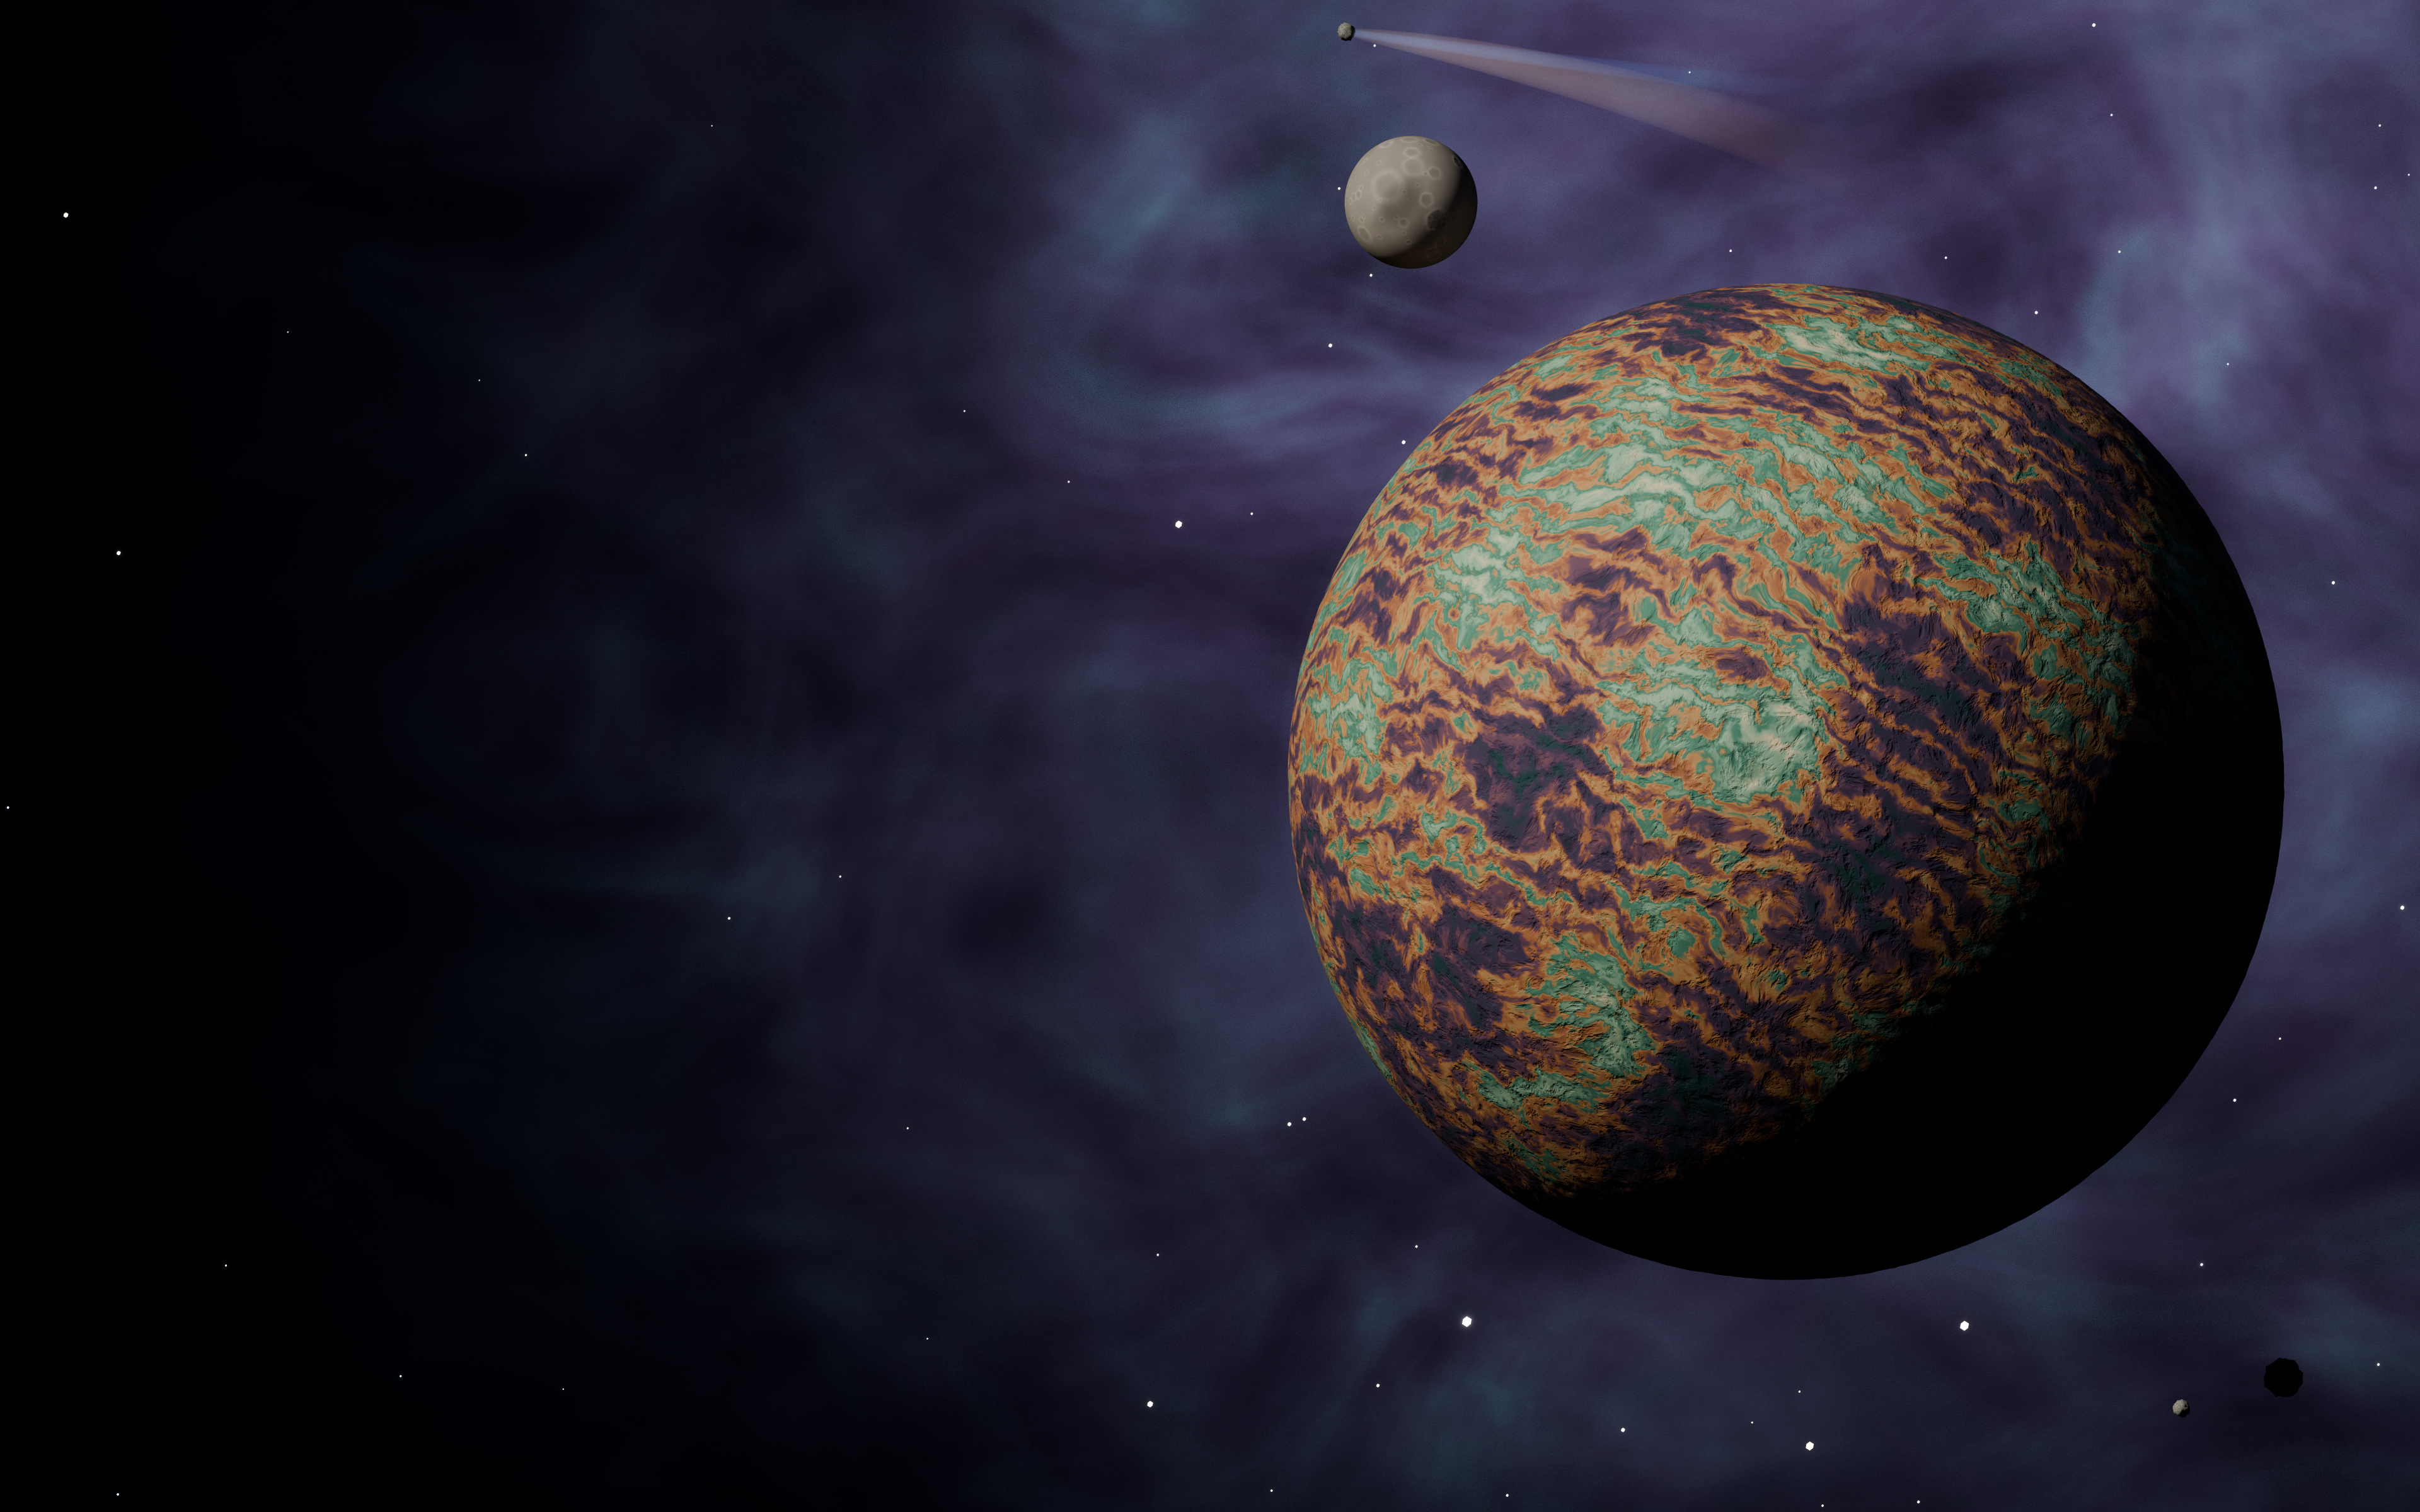
\includegraphics[width=20cm,height=12.5cm]{Risorse/Copertine/M08_Polychroma.jpg}};}{}
\node[anchor=north west,inner sep=0] at([xshift=1.05cm,yshift=-1.10cm]current page.north west){\color{Mint}\bfseries\fontsize{23}{28}\selectfont POLYCHROMA};
\node[anchor=north west,inner sep=0] at([xshift=1.07cm,yshift=-2.16cm]current page.north west){\color{white}\fontsize{9}{12}\selectfont MODULO M08 · SCIENZE DELLA TERRA};
\draw[Mint,line width=1.5pt]([xshift=1.07cm,yshift=-2.78cm]current page.north west)--([xshift=2.6cm,yshift=-2.78cm]current page.north west);
\node[anchor=north west,inner sep=0] at([xshift=1.05cm,yshift=-3.35cm]current page.north west){\begin{minipage}{9.2cm}\raggedright\color{white}\bfseries\fontsize{30}{36}\selectfont Analisi\\multivariata\\dei campioni\end{minipage}};
\node[anchor=north west,inner sep=0] at([xshift=1.07cm,yshift=-7.88cm]current page.north west){\begin{minipage}{8.9cm}\raggedright\color{Lilac}\fontsize{12.2}{17}\selectfont Geometria della PCA,\\partizioni e interpretazione geologica\end{minipage}};
\node[anchor=north west,inner sep=0] at([xshift=1.07cm,yshift=-10.52cm]current page.north west){\color{white}\fontsize{11.5}{15}\selectfont Marzio De Corato};
\node[anchor=north west,inner sep=0] at([xshift=1.07cm,yshift=-11.17cm]current page.north west){\color{Mint}\fontsize{8.8}{11}\selectfont\href{https://creativecommons.org/licenses/by-nc-sa/4.0/}{© 2026 · CC BY-NC-SA 4.0}};
\end{tikzpicture}\end{frame}
\begin{frame}[plain]\hypertarget{slide2}{}
\bookmark[level=0,page=2]{Campioni, scale e distanze}
\bookmark[level=1,page=2]{Quali campioni si somigliano?}
\begin{lrbox}{\PilotLeftBox}%
\begin{minipage}[t]{10.05cm}\raggedright\color{Ink}\fontsize{11.3}{14.8}\selectfont
\PLabel{Una stessa matrice, più proprietà}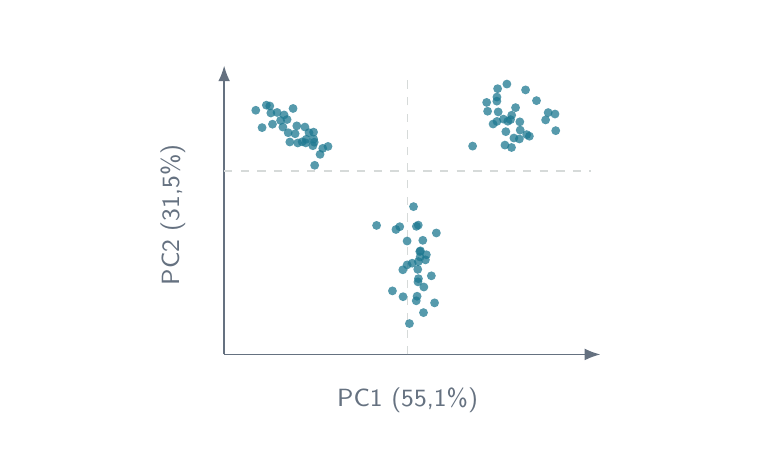
\begin{tikzpicture}[x=1cm,y=1cm]
\path[use as bounding box](-.15,-.2) rectangle(9.1,4.8500000000000005);
\draw[pAxis](2.3453125000000004,0.7)--(7.1246875,0.7);
\draw[pAxis](2.3453125000000004,0.7)--(2.3453125000000004,4.37);
\node[pNote] at(4.675000000000001,0.12){PC1 (55{,}1\%)};
\node[pNote,rotate=90] at(1.6953125000000004,2.475){PC2 (31{,}5\%)};
\draw[Rule,dashed] plot coordinates {(4.6750,0.7000) (4.6750,4.2500)};
\draw[Rule,dashed] plot coordinates {(2.3453,3.0297) (7.0047,3.0297)};
\fill[GeoA,opacity=.75](3.3710,3.5877) circle(1.6pt);
\fill[GeoA,opacity=.75](2.8814,3.8658) circle(1.6pt);
\fill[GeoA,opacity=.75](3.1796,3.3982) circle(1.6pt);
\fill[GeoA,opacity=.75](3.2465,3.5028) circle(1.6pt);
\fill[GeoA,opacity=.75](3.0617,3.6715) circle(1.6pt);
\fill[GeoA,opacity=.75](3.4720,3.3508) circle(1.6pt);
\fill[GeoA,opacity=.75](3.1584,3.5162) circle(1.6pt);
\fill[GeoA,opacity=.75](3.1063,3.7418) circle(1.6pt);
\fill[GeoA,opacity=.75](3.2678,3.6029) circle(1.6pt);
\fill[GeoA,opacity=.75](2.8270,3.5807) circle(1.6pt);
\fill[GeoA,opacity=.75](3.5976,3.3173) circle(1.6pt);
\fill[GeoA,opacity=.75](2.9383,3.7663) circle(1.6pt);
\fill[GeoA,opacity=.75](3.4949,3.1020) circle(1.6pt);
\fill[GeoA,opacity=.75](3.3358,3.4005) circle(1.6pt);
\fill[GeoA,opacity=.75](3.6642,3.3419) circle(1.6pt);
\fill[GeoA,opacity=.75](3.5634,3.2414) circle(1.6pt);
\fill[GeoA,opacity=.75](3.1445,3.6832) circle(1.6pt);
\fill[GeoA,opacity=.75](3.0912,3.5875) circle(1.6pt);
\fill[GeoA,opacity=.75](3.4807,3.5232) circle(1.6pt);
\fill[GeoA,opacity=.75](3.3820,3.3867) circle(1.6pt);
\fill[GeoA,opacity=.75](3.4230,3.5162) circle(1.6pt);
\fill[GeoA,opacity=.75](2.9252,3.8553) circle(1.6pt);
\fill[GeoA,opacity=.75](3.0177,3.7734) circle(1.6pt);
\fill[GeoA,opacity=.75](3.2799,3.3858) circle(1.6pt);
\fill[GeoA,opacity=.75](3.4895,3.3955) circle(1.6pt);
\fill[GeoA,opacity=.75](3.2204,3.8238) circle(1.6pt);
\fill[GeoA,opacity=.75](3.4821,3.4350) circle(1.6pt);
\fill[GeoA,opacity=.75](2.9592,3.6243) circle(1.6pt);
\fill[GeoA,opacity=.75](2.7470,3.8011) circle(1.6pt);
\fill[GeoA,opacity=.75](3.3880,3.4327) circle(1.6pt);
\fill[GeoA,opacity=.75](4.6982,1.0923) circle(1.6pt);
\fill[GeoA,opacity=.75](4.7867,2.3271) circle(1.6pt);
\fill[GeoA,opacity=.75](4.6688,2.1404) circle(1.6pt);
\fill[GeoA,opacity=.75](4.6144,1.7750) circle(1.6pt);
\fill[GeoA,opacity=.75](4.8345,1.9372) circle(1.6pt);
\fill[GeoA,opacity=.75](5.0176,1.3549) circle(1.6pt);
\fill[GeoA,opacity=.75](4.8814,1.5564) circle(1.6pt);
\fill[GeoA,opacity=.75](4.8300,2.0069) circle(1.6pt);
\fill[GeoA,opacity=.75](4.6692,1.8374) circle(1.6pt);
\fill[GeoA,opacity=.75](4.5753,2.3222) circle(1.6pt);
\fill[GeoA,opacity=.75](4.4825,1.5070) circle(1.6pt);
\fill[GeoA,opacity=.75](4.9134,1.9664) circle(1.6pt);
\fill[GeoA,opacity=.75](4.8127,1.6625) circle(1.6pt);
\fill[GeoA,opacity=.75](4.8683,2.1492) circle(1.6pt);
\fill[GeoA,opacity=.75](4.7847,1.3814) circle(1.6pt);
\fill[GeoA,opacity=.75](4.2812,2.3386) circle(1.6pt);
\fill[GeoA,opacity=.75](4.8115,1.8793) circle(1.6pt);
\fill[GeoA,opacity=.75](4.9768,1.6985) circle(1.6pt);
\fill[GeoA,opacity=.75](4.7502,2.5774) circle(1.6pt);
\fill[GeoA,opacity=.75](4.8042,1.7807) circle(1.6pt);
\fill[GeoA,opacity=.75](5.0402,2.2427) circle(1.6pt);
\fill[GeoA,opacity=.75](4.7959,1.4393) circle(1.6pt);
\fill[GeoA,opacity=.75](4.9013,1.9009) circle(1.6pt);
\fill[GeoA,opacity=.75](4.8107,2.3423) circle(1.6pt);
\fill[GeoA,opacity=.75](4.5268,2.2869) circle(1.6pt);
\fill[GeoA,opacity=.75](4.7332,1.8587) circle(1.6pt);
\fill[GeoA,opacity=.75](4.8379,2.0155) circle(1.6pt);
\fill[GeoA,opacity=.75](4.6173,1.4333) circle(1.6pt);
\fill[GeoA,opacity=.75](4.8769,1.2314) circle(1.6pt);
\fill[GeoA,opacity=.75](4.8069,1.6219) circle(1.6pt);
\fill[GeoA,opacity=.75](5.6791,3.9007) circle(1.6pt);
\fill[GeoA,opacity=.75](6.4278,3.6785) circle(1.6pt);
\fill[GeoA,opacity=.75](5.8253,3.7802) circle(1.6pt);
\fill[GeoA,opacity=.75](6.5470,3.7532) circle(1.6pt);
\fill[GeoA,opacity=.75](5.8097,3.9688) circle(1.6pt);
\fill[GeoA,opacity=.75](5.9112,3.3587) circle(1.6pt);
\fill[GeoA,opacity=.75](6.1732,4.0596) circle(1.6pt);
\fill[GeoA,opacity=.75](5.8184,4.0751) circle(1.6pt);
\fill[GeoA,opacity=.75](5.9971,3.7384) circle(1.6pt);
\fill[GeoA,opacity=.75](5.8087,3.9167) circle(1.6pt);
\fill[GeoA,opacity=.75](6.1878,3.4917) circle(1.6pt);
\fill[GeoA,opacity=.75](5.6912,3.7888) circle(1.6pt);
\fill[GeoA,opacity=.75](6.3122,3.9233) circle(1.6pt);
\fill[GeoA,opacity=.75](5.8921,3.6887) circle(1.6pt);
\fill[GeoA,opacity=.75](6.0250,3.4485) circle(1.6pt);
\fill[GeoA,opacity=.75](6.1053,3.5492) circle(1.6pt);
\fill[GeoA,opacity=.75](5.9228,3.5293) circle(1.6pt);
\fill[GeoA,opacity=.75](5.9819,3.6819) circle(1.6pt);
\fill[GeoA,opacity=.75](6.1003,3.6539) circle(1.6pt);
\fill[GeoA,opacity=.75](5.9360,4.1338) circle(1.6pt);
\fill[GeoA,opacity=.75](5.9947,3.3283) circle(1.6pt);
\fill[GeoA,opacity=.75](6.0945,3.4365) circle(1.6pt);
\fill[GeoA,opacity=.75](6.2219,3.4717) circle(1.6pt);
\fill[GeoA,opacity=.75](5.8097,3.6594) circle(1.6pt);
\fill[GeoA,opacity=.75](5.9474,3.6616) circle(1.6pt);
\fill[GeoA,opacity=.75](6.0461,3.8345) circle(1.6pt);
\fill[GeoA,opacity=.75](5.7607,3.6264) circle(1.6pt);
\fill[GeoA,opacity=.75](5.5009,3.3459) circle(1.6pt);
\fill[GeoA,opacity=.75](6.5562,3.5420) circle(1.6pt);
\fill[GeoA,opacity=.75](6.4603,3.7716) circle(1.6pt);
\end{tikzpicture}\PSmall{I punti rappresentano le 90 rocce sintetiche proiettate sulle prime due componenti. I colori dei gruppi non sono ancora assegnati.}
\end{minipage}%
\end{lrbox}
\typeout{FULLBOX:002:L:\the\ht\PilotLeftBox:\the\dp\PilotLeftBox}
\begin{lrbox}{\PilotRightBox}%
\begin{minipage}[t]{7.55cm}\raggedright\color{Ink}\fontsize{11.3}{14.8}\selectfont

\PBody{Ogni roccia è descritta da otto misure. La somiglianza dipende da quali proprietà confrontiamo e da come misuriamo le loro differenze.}
\vspace{4mm}
\[\mathbf x_i=(x_{i1},\ldots,x_{i8}).\]
\PInfo{La domanda della lezione: quali strutture persistono quando cambiamo rappresentazione, variabili o criterio di raggruppamento?}
\vspace{3mm}
\PBody{PCA e clustering richiedono scelte esplicite. L’interpretazione geologica viene discussa attraverso queste scelte.}

\end{minipage}%
\end{lrbox}
\typeout{FULLBOX:002:R:\the\ht\PilotRightBox:\the\dp\PilotRightBox}
\begin{tikzpicture}[remember picture,overlay]
\PilotChrome{Quali campioni si somigliano?}{I · CAMPIONI, SCALE E DISTANZE}{2}{Una struttura multivariata si interpreta insieme alle misure e alla geometria che l’hanno prodotta.}
\node[anchor=north west,inner sep=0] at([xshift=0.96cm,yshift=-2.13cm]current page.north west){\usebox{\PilotLeftBox}};
\node[anchor=north west,inner sep=0] at([xshift=11.52cm,yshift=-2.13cm]current page.north west){\usebox{\PilotRightBox}};
\end{tikzpicture}\end{frame}

\begin{frame}[plain]\hypertarget{slide3}{}
\bookmark[level=1,page=3]{Novanta rocce, otto proprietà}
\begin{lrbox}{\PilotLeftBox}%
\begin{minipage}[t]{10.05cm}\raggedright\color{Ink}\fontsize{11.3}{14.8}\selectfont
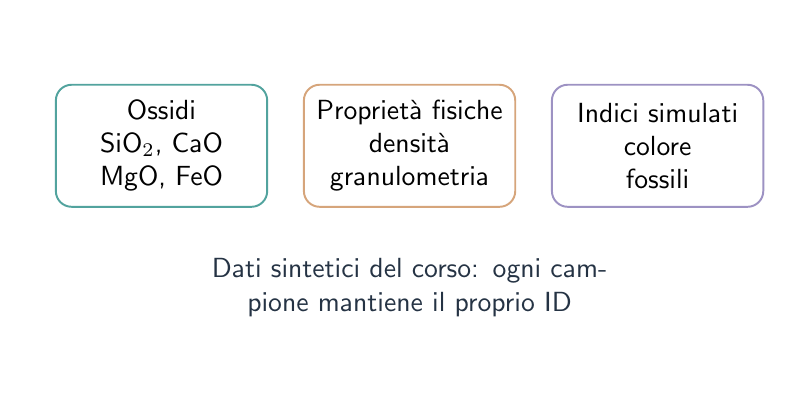
\begin{tikzpicture}[x=1cm,y=1cm]
\path[use as bounding box](-.15,-.15) rectangle(9.4,4.2);
\node[pFlow,draw=Classical!70,text width=2.45cm,minimum height=1.55cm] at(1.55,2.7){Ossidi\\SiO$_2$, CaO\\MgO, FeO};\node[pFlow,draw=GeoB!70,text width=2.45cm,minimum height=1.55cm] at(4.7,2.7){Proprietà fisiche\\densità\\granulometria};\node[pFlow,draw=GeoC!70,text width=2.45cm,minimum height=1.55cm] at(7.85,2.7){Indici simulati\\colore\\fossili};\node[pLabel,text width=8.6cm] at(4.7,.9){Dati sintetici del corso: ogni campione mantiene il proprio ID};
\end{tikzpicture}\PBody{Il dataset comprende 90 campioni. Le etichette generatrici sono Basalto, Arenaria e Calcare: trenta casi per gruppo.}
\end{minipage}%
\end{lrbox}
\typeout{FULLBOX:003:L:\the\ht\PilotLeftBox:\the\dp\PilotLeftBox}
\begin{lrbox}{\PilotRightBox}%
\begin{minipage}[t]{7.55cm}\raggedright\color{Ink}\fontsize{11.3}{14.8}\selectfont
\PCode{R · leggere i campioni}{003_dati.R}\PInfo{Colore e fossili sono indici convenzionali del simulatore. I valori non descrivono misure di un affioramento reale.}
\end{minipage}%
\end{lrbox}
\typeout{FULLBOX:003:R:\the\ht\PilotRightBox:\the\dp\PilotRightBox}
\begin{tikzpicture}[remember picture,overlay]
\PilotChrome{Novanta rocce, otto proprietà}{I · CAMPIONI, SCALE E DISTANZE}{3}{Il significato di ogni colonna e la provenienza sintetica dei dati devono accompagnare l’analisi.}
\node[anchor=north west,inner sep=0] at([xshift=0.96cm,yshift=-2.13cm]current page.north west){\usebox{\PilotLeftBox}};
\node[anchor=north west,inner sep=0] at([xshift=11.52cm,yshift=-2.13cm]current page.north west){\usebox{\PilotRightBox}};
\end{tikzpicture}\end{frame}

\begin{frame}[plain]\hypertarget{slide4}{}
\bookmark[level=1,page=4]{La matrice conserva le righe dei campioni}
\begin{lrbox}{\PilotLeftBox}%
\begin{minipage}[t]{10.05cm}\raggedright\color{Ink}\fontsize{11.3}{14.8}\selectfont
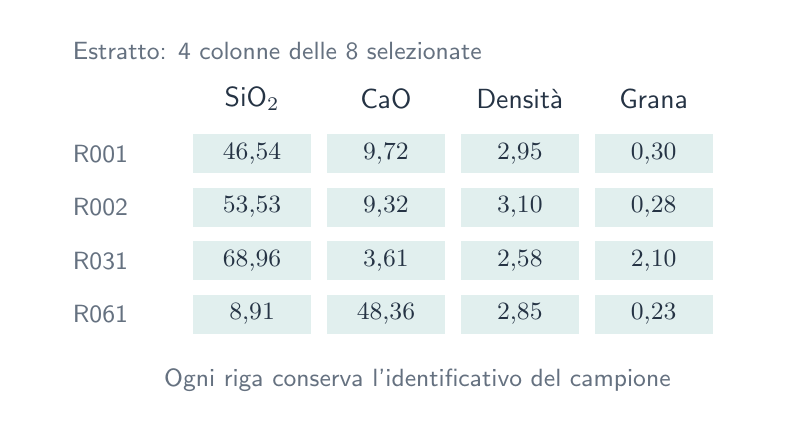
\begin{tikzpicture}[x=1cm,y=1cm]
\path[use as bounding box](-.15,-.15) rectangle(9.4,4.6);
\node[pNote,anchor=west] at(.3,4.3){Estratto: 4 colonne delle 8 selezionate};\node[pLabel] at(2.7,3.7){SiO$_2$};\node[pLabel] at(4.4,3.7){CaO};\node[pLabel] at(6.1,3.7){Densità};\node[pLabel] at(7.8,3.7){Grana};\node[pNote,anchor=west] at(.3,3.0){R001};\fill[Classical!12](1.95,2.75) rectangle(3.45,3.25);\node[pNote,text=Ink] at(2.7,3.0){$ 46{,}54 $};\fill[Classical!12](3.65,2.75) rectangle(5.15,3.25);\node[pNote,text=Ink] at(4.4,3.0){$ 9{,}72 $};\fill[Classical!12](5.35,2.75) rectangle(6.85,3.25);\node[pNote,text=Ink] at(6.1,3.0){$ 2{,}95 $};\fill[Classical!12](7.05,2.75) rectangle(8.55,3.25);\node[pNote,text=Ink] at(7.8,3.0){$ 0{,}30 $};\node[pNote,anchor=west] at(.3,2.32){R002};\fill[Classical!12](1.95,2.07) rectangle(3.45,2.57);\node[pNote,text=Ink] at(2.7,2.32){$ 53{,}53 $};\fill[Classical!12](3.65,2.07) rectangle(5.15,2.57);\node[pNote,text=Ink] at(4.4,2.32){$ 9{,}32 $};\fill[Classical!12](5.35,2.07) rectangle(6.85,2.57);\node[pNote,text=Ink] at(6.1,2.32){$ 3{,}10 $};\fill[Classical!12](7.05,2.07) rectangle(8.55,2.57);\node[pNote,text=Ink] at(7.8,2.32){$ 0{,}28 $};\node[pNote,anchor=west] at(.3,1.64){R031};\fill[Classical!12](1.95,1.39) rectangle(3.45,1.89);\node[pNote,text=Ink] at(2.7,1.64){$ 68{,}96 $};\fill[Classical!12](3.65,1.39) rectangle(5.15,1.89);\node[pNote,text=Ink] at(4.4,1.64){$ 3{,}61 $};\fill[Classical!12](5.35,1.39) rectangle(6.85,1.89);\node[pNote,text=Ink] at(6.1,1.64){$ 2{,}58 $};\fill[Classical!12](7.05,1.39) rectangle(8.55,1.89);\node[pNote,text=Ink] at(7.8,1.64){$ 2{,}10 $};\node[pNote,anchor=west] at(.3,0.96){R061};\fill[Classical!12](1.95,0.71) rectangle(3.45,1.21);\node[pNote,text=Ink] at(2.7,0.96){$ 8{,}91 $};\fill[Classical!12](3.65,0.71) rectangle(5.15,1.21);\node[pNote,text=Ink] at(4.4,0.96){$ 48{,}36 $};\fill[Classical!12](5.35,0.71) rectangle(6.85,1.21);\node[pNote,text=Ink] at(6.1,0.96){$ 2{,}85 $};\fill[Classical!12](7.05,0.71) rectangle(8.55,1.21);\node[pNote,text=Ink] at(7.8,0.96){$ 0{,}23 $};\node[pNote] at(4.8,.12){Ogni riga conserva l’identificativo del campione};
\end{tikzpicture}\[X=(x_{ij})\in\mathbb R^{90\times8}.\]
\end{minipage}%
\end{lrbox}
\typeout{FULLBOX:004:L:\the\ht\PilotLeftBox:\the\dp\PilotLeftBox}
\begin{lrbox}{\PilotRightBox}%
\begin{minipage}[t]{7.55cm}\raggedright\color{Ink}\fontsize{11.3}{14.8}\selectfont

\PBody{L’indice $i$ identifica il campione; $j$ identifica la variabile. Una riga confronta più proprietà della stessa roccia.}
\vspace{4mm}
\PInfo{Una colonna contiene misure omogenee per definizione e unità. L’identificativo rimane esterno alla matrice numerica.}
\vspace{3mm}
\PBody{Conservare l’ordine delle righe consente di ricongiungere coordinate principali, gruppi e osservazioni originali.}

\end{minipage}%
\end{lrbox}
\typeout{FULLBOX:004:R:\the\ht\PilotRightBox:\the\dp\PilotRightBox}
\begin{tikzpicture}[remember picture,overlay]
\PilotChrome{La matrice conserva le righe dei campioni}{I · CAMPIONI, SCALE E DISTANZE}{4}{Il punto nello spazio multivariato corrisponde a una riga identificabile della tabella.}
\node[anchor=north west,inner sep=0] at([xshift=0.96cm,yshift=-2.13cm]current page.north west){\usebox{\PilotLeftBox}};
\node[anchor=north west,inner sep=0] at([xshift=11.52cm,yshift=-2.13cm]current page.north west){\usebox{\PilotRightBox}};
\end{tikzpicture}\end{frame}

\begin{frame}[plain]\hypertarget{slide5}{}
\bookmark[level=1,page=5]{Le unità definiscono le coordinate}
\begin{lrbox}{\PilotLeftBox}%
\begin{minipage}[t]{10.05cm}\raggedright\color{Ink}\fontsize{11.3}{14.8}\selectfont
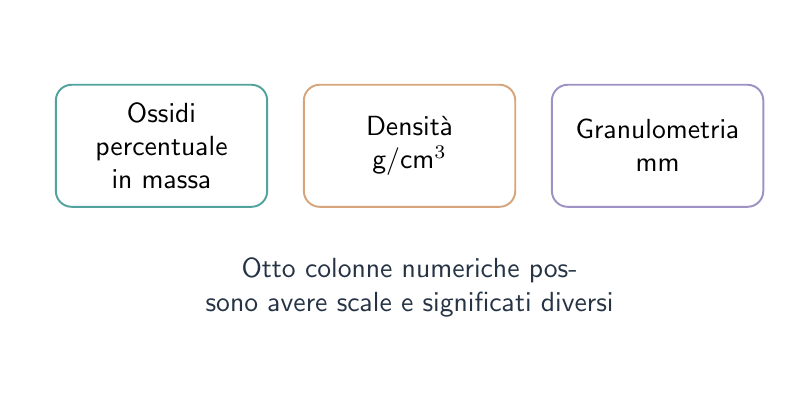
\begin{tikzpicture}[x=1cm,y=1cm]
\path[use as bounding box](-.15,-.15) rectangle(9.4,4.2);
\node[pFlow,draw=Classical!70,text width=2.45cm,minimum height=1.55cm] at(1.55,2.7){Ossidi\\percentuale in massa};\node[pFlow,draw=GeoB!70,text width=2.45cm,minimum height=1.55cm] at(4.7,2.7){Densità\\g/cm$^3$};\node[pFlow,draw=GeoC!70,text width=2.45cm,minimum height=1.55cm] at(7.85,2.7){Granulometria\\mm};\node[pLabel,text width=8.6cm] at(4.7,.9){Otto colonne numeriche possono avere scale e significati diversi};
\end{tikzpicture}\PBody{Una differenza di dieci punti percentuali e una differenza di un grammo per centimetro cubo non hanno un peso naturale comune.}
\end{minipage}%
\end{lrbox}
\typeout{FULLBOX:005:L:\the\ht\PilotLeftBox:\the\dp\PilotLeftBox}
\begin{lrbox}{\PilotRightBox}%
\begin{minipage}[t]{7.55cm}\raggedright\color{Ink}\fontsize{11.3}{14.8}\selectfont

\[\mathbf x_i=(\text{SiO}_2,\ldots,\rho,g,c,f)_i.\]
\PBody{La somma dei quadrati combina valori numerici. Le conversioni di unità possono modificare il contributo di una proprietà alla distanza.}
\vspace{3mm}
\PInfo{Prima della standardizzazione, occorre stabilire quali differenze scientifiche debbano contare nella somiglianza.}

\end{minipage}%
\end{lrbox}
\typeout{FULLBOX:005:R:\the\ht\PilotRightBox:\the\dp\PilotRightBox}
\begin{tikzpicture}[remember picture,overlay]
\PilotChrome{Le unità definiscono le coordinate}{I · CAMPIONI, SCALE E DISTANZE}{5}{Una distanza fra variabili eterogenee incorpora una scelta di scala e di rilevanza.}
\node[anchor=north west,inner sep=0] at([xshift=0.96cm,yshift=-2.13cm]current page.north west){\usebox{\PilotLeftBox}};
\node[anchor=north west,inner sep=0] at([xshift=11.52cm,yshift=-2.13cm]current page.north west){\usebox{\PilotRightBox}};
\end{tikzpicture}\end{frame}

\begin{frame}[plain]\hypertarget{slide6}{}
\bookmark[level=1,page=6]{Misure, identificativi ed etichette}
\begin{lrbox}{\PilotLeftBox}%
\begin{minipage}[t]{10.05cm}\raggedright\color{Ink}\fontsize{11.3}{14.8}\selectfont
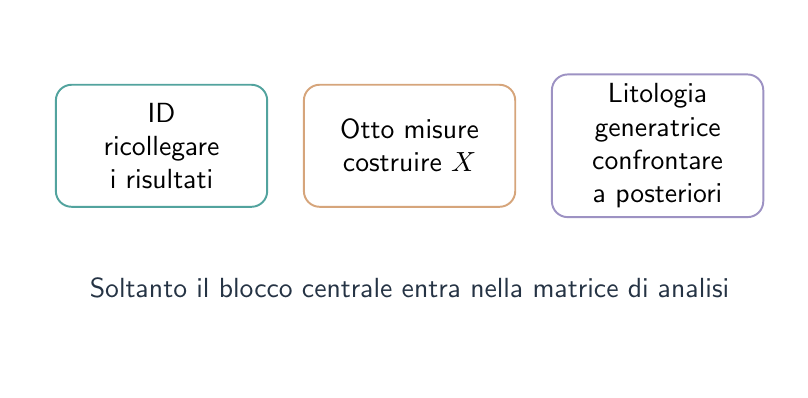
\begin{tikzpicture}[x=1cm,y=1cm]
\path[use as bounding box](-.15,-.15) rectangle(9.4,4.2);
\node[pFlow,draw=Classical!70,text width=2.45cm,minimum height=1.55cm] at(1.55,2.7){ID\\ricollegare i risultati};\node[pFlow,draw=GeoB!70,text width=2.45cm,minimum height=1.55cm] at(4.7,2.7){Otto misure\\costruire $X$};\node[pFlow,draw=GeoC!70,text width=2.45cm,minimum height=1.55cm] at(7.85,2.7){Litologia generatrice\\confrontare a posteriori};\node[pLabel,text width=8.6cm] at(4.7,.9){Soltanto il blocco centrale entra nella matrice di analisi};
\end{tikzpicture}\PBody{L’etichetta del simulatore è tenuta separata. Usarla come una coordinata introdurrebbe la risposta attesa nel criterio di somiglianza.}
\end{minipage}%
\end{lrbox}
\typeout{FULLBOX:006:L:\the\ht\PilotLeftBox:\the\dp\PilotLeftBox}
\begin{lrbox}{\PilotRightBox}%
\begin{minipage}[t]{7.55cm}\raggedright\color{Ink}\fontsize{11.3}{14.8}\selectfont
\PCode{R · separare i ruoli}{006_etichette.R}\PSmall{Le etichette potranno colorare un grafico già calcolato o alimentare una tabella di confronto.}
\end{minipage}%
\end{lrbox}
\typeout{FULLBOX:006:R:\the\ht\PilotRightBox:\the\dp\PilotRightBox}
\begin{tikzpicture}[remember picture,overlay]
\PilotChrome{Misure, identificativi ed etichette}{I · CAMPIONI, SCALE E DISTANZE}{6}{Una variabile usata per interpretare il risultato può restare esclusa dal calcolo dei gruppi.}
\node[anchor=north west,inner sep=0] at([xshift=0.96cm,yshift=-2.13cm]current page.north west){\usebox{\PilotLeftBox}};
\node[anchor=north west,inner sep=0] at([xshift=11.52cm,yshift=-2.13cm]current page.north west){\usebox{\PilotRightBox}};
\end{tikzpicture}\end{frame}

\begin{frame}[plain]\hypertarget{slide7}{}
\bookmark[level=1,page=7]{Selezionare le variabili per nome}
\begin{lrbox}{\PilotLeftBox}%
\begin{minipage}[t]{10.05cm}\raggedright\color{Ink}\fontsize{11.3}{14.8}\selectfont
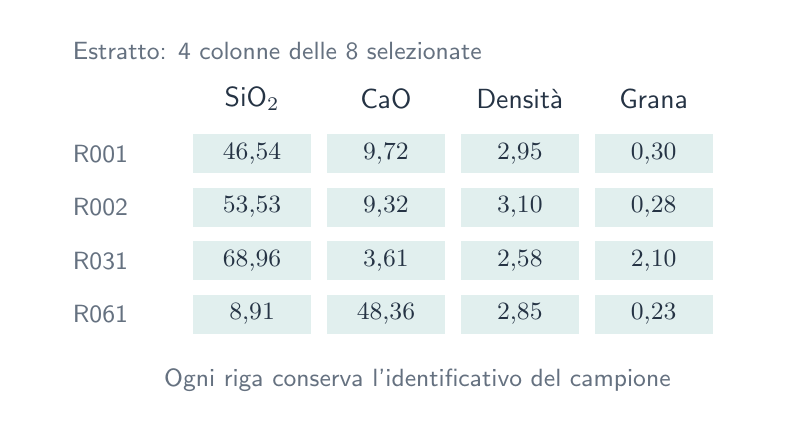
\begin{tikzpicture}[x=1cm,y=1cm]
\path[use as bounding box](-.15,-.15) rectangle(9.4,4.6);
\node[pNote,anchor=west] at(.3,4.3){Estratto: 4 colonne delle 8 selezionate};\node[pLabel] at(2.7,3.7){SiO$_2$};\node[pLabel] at(4.4,3.7){CaO};\node[pLabel] at(6.1,3.7){Densità};\node[pLabel] at(7.8,3.7){Grana};\node[pNote,anchor=west] at(.3,3.0){R001};\fill[Classical!12](1.95,2.75) rectangle(3.45,3.25);\node[pNote,text=Ink] at(2.7,3.0){$ 46{,}54 $};\fill[Classical!12](3.65,2.75) rectangle(5.15,3.25);\node[pNote,text=Ink] at(4.4,3.0){$ 9{,}72 $};\fill[Classical!12](5.35,2.75) rectangle(6.85,3.25);\node[pNote,text=Ink] at(6.1,3.0){$ 2{,}95 $};\fill[Classical!12](7.05,2.75) rectangle(8.55,3.25);\node[pNote,text=Ink] at(7.8,3.0){$ 0{,}30 $};\node[pNote,anchor=west] at(.3,2.32){R002};\fill[Classical!12](1.95,2.07) rectangle(3.45,2.57);\node[pNote,text=Ink] at(2.7,2.32){$ 53{,}53 $};\fill[Classical!12](3.65,2.07) rectangle(5.15,2.57);\node[pNote,text=Ink] at(4.4,2.32){$ 9{,}32 $};\fill[Classical!12](5.35,2.07) rectangle(6.85,2.57);\node[pNote,text=Ink] at(6.1,2.32){$ 3{,}10 $};\fill[Classical!12](7.05,2.07) rectangle(8.55,2.57);\node[pNote,text=Ink] at(7.8,2.32){$ 0{,}28 $};\node[pNote,anchor=west] at(.3,1.64){R031};\fill[Classical!12](1.95,1.39) rectangle(3.45,1.89);\node[pNote,text=Ink] at(2.7,1.64){$ 68{,}96 $};\fill[Classical!12](3.65,1.39) rectangle(5.15,1.89);\node[pNote,text=Ink] at(4.4,1.64){$ 3{,}61 $};\fill[Classical!12](5.35,1.39) rectangle(6.85,1.89);\node[pNote,text=Ink] at(6.1,1.64){$ 2{,}58 $};\fill[Classical!12](7.05,1.39) rectangle(8.55,1.89);\node[pNote,text=Ink] at(7.8,1.64){$ 2{,}10 $};\node[pNote,anchor=west] at(.3,0.96){R061};\fill[Classical!12](1.95,0.71) rectangle(3.45,1.21);\node[pNote,text=Ink] at(2.7,0.96){$ 8{,}91 $};\fill[Classical!12](3.65,0.71) rectangle(5.15,1.21);\node[pNote,text=Ink] at(4.4,0.96){$ 48{,}36 $};\fill[Classical!12](5.35,0.71) rectangle(6.85,1.21);\node[pNote,text=Ink] at(6.1,0.96){$ 2{,}85 $};\fill[Classical!12](7.05,0.71) rectangle(8.55,1.21);\node[pNote,text=Ink] at(7.8,0.96){$ 0{,}23 $};\node[pNote] at(4.8,.12){Ogni riga conserva l’identificativo del campione};
\end{tikzpicture}\PBody{La selezione esplicita rende leggibile la scelta delle proprietà. L’ordine delle colonne è conservato nelle trasformazioni successive.}
\end{minipage}%
\end{lrbox}
\typeout{FULLBOX:007:L:\the\ht\PilotLeftBox:\the\dp\PilotLeftBox}
\begin{lrbox}{\PilotRightBox}%
\begin{minipage}[t]{7.55cm}\raggedright\color{Ink}\fontsize{11.3}{14.8}\selectfont
\PCode{R · costruire la matrice}{007_matrice.R}\PInfo{I controlli numerici verificano completezza e variabilità. La scelta scientifica delle colonne richiede comunque una motivazione.}
\end{minipage}%
\end{lrbox}
\typeout{FULLBOX:007:R:\the\ht\PilotRightBox:\the\dp\PilotRightBox}
\begin{tikzpicture}[remember picture,overlay]
\PilotChrome{Selezionare le variabili per nome}{I · CAMPIONI, SCALE E DISTANZE}{7}{Un dataset leggibile da R può ancora contenere colonne inappropriate per la domanda.}
\node[anchor=north west,inner sep=0] at([xshift=0.96cm,yshift=-2.13cm]current page.north west){\usebox{\PilotLeftBox}};
\node[anchor=north west,inner sep=0] at([xshift=11.52cm,yshift=-2.13cm]current page.north west){\usebox{\PilotRightBox}};
\end{tikzpicture}\end{frame}

\begin{frame}[plain]\hypertarget{slide8}{}
\bookmark[level=1,page=8]{La scala cambia la geometria}
\begin{lrbox}{\PilotLeftBox}%
\begin{minipage}[t]{10.05cm}\raggedright\color{Ink}\fontsize{11.3}{14.8}\selectfont
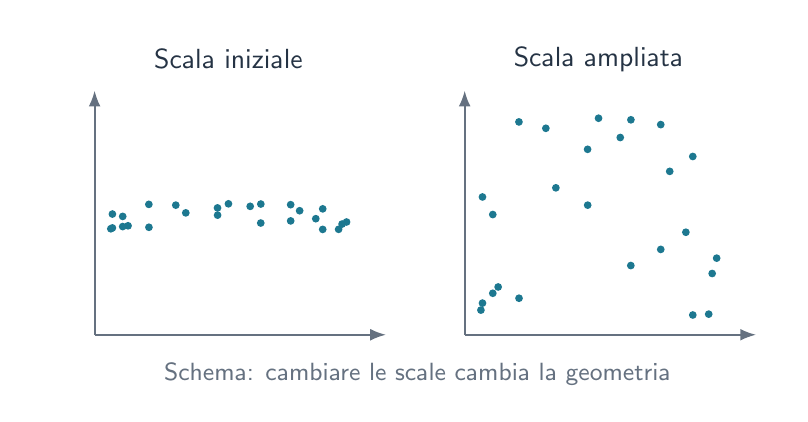
\begin{tikzpicture}[x=1cm,y=1cm]
\path[use as bounding box](-.15,-.15) rectangle(9.4,4.5);
\draw[pAxis](0.7,.6)--(4.4,.6);\draw[pAxis](0.7,.6)--(0.7,3.7);\fill[GeoA](2.400,2.263) circle(1.4pt);\fill[GeoA](3.509,2.074) circle(1.4pt);\fill[GeoA](0.906,1.946) circle(1.4pt);\fill[GeoA](3.304,2.175) circle(1.4pt);\fill[GeoA](2.676,2.231) circle(1.4pt);\fill[GeoA](1.125,1.984) circle(1.4pt);\fill[GeoA](3.843,2.006) circle(1.4pt);\fill[GeoA](1.731,2.246) circle(1.4pt);\fill[GeoA](1.858,2.148) circle(1.4pt);\fill[GeoA](3.799,1.939) circle(1.4pt);\fill[GeoA](1.057,2.103) circle(1.4pt);\fill[GeoA](2.811,2.260) circle(1.4pt);\fill[GeoA](3.190,2.046) circle(1.4pt);\fill[GeoA](0.926,1.957) circle(1.4pt);\fill[GeoA](3.597,2.199) circle(1.4pt);\fill[GeoA](2.261,2.211) circle(1.4pt);\fill[GeoA](1.390,1.965) circle(1.4pt);\fill[GeoA](3.900,2.032) circle(1.4pt);\fill[GeoA](1.389,2.256) circle(1.4pt);\fill[GeoA](2.262,2.119) circle(1.4pt);\fill[GeoA](3.597,1.938) circle(1.4pt);\fill[GeoA](0.926,2.133) circle(1.4pt);\fill[GeoA](3.190,2.252) circle(1.4pt);\fill[GeoA](2.810,2.019) circle(1.4pt);\fill[GeoA](1.057,1.974) circle(1.4pt);\node[pLabel] at(2.4,4.1){Scala iniziale};\draw[pAxis](5.4,.6)--(9.100000000000001,.6);\draw[pAxis](5.4,.6)--(5.4,3.7);\fill[GeoA](7.100,3.350) circle(1.4pt);\fill[GeoA](8.209,1.902) circle(1.4pt);\fill[GeoA](5.606,0.913) circle(1.4pt);\fill[GeoA](8.004,2.675) circle(1.4pt);\fill[GeoA](7.376,3.105) circle(1.4pt);\fill[GeoA](5.825,1.207) circle(1.4pt);\fill[GeoA](8.543,1.378) circle(1.4pt);\fill[GeoA](6.431,3.222) circle(1.4pt);\fill[GeoA](6.558,2.466) circle(1.4pt);\fill[GeoA](8.499,0.862) circle(1.4pt);\fill[GeoA](5.757,2.127) circle(1.4pt);\fill[GeoA](7.511,3.330) circle(1.4pt);\fill[GeoA](7.890,1.684) circle(1.4pt);\fill[GeoA](5.626,1.002) circle(1.4pt);\fill[GeoA](8.297,2.864) circle(1.4pt);\fill[GeoA](6.961,2.955) circle(1.4pt);\fill[GeoA](6.090,1.064) circle(1.4pt);\fill[GeoA](8.600,1.573) circle(1.4pt);\fill[GeoA](6.089,3.303) circle(1.4pt);\fill[GeoA](6.962,2.246) circle(1.4pt);\fill[GeoA](8.297,0.851) circle(1.4pt);\fill[GeoA](5.626,2.350) circle(1.4pt);\fill[GeoA](7.890,3.269) circle(1.4pt);\fill[GeoA](7.510,1.479) circle(1.4pt);\fill[GeoA](5.757,1.127) circle(1.4pt);\node[pLabel] at(7.1000000000000005,4.1){Scala ampliata};\node[pNote] at(4.8,.1){Schema: cambiare le scale cambia la geometria};
\end{tikzpicture}\PBody{Moltiplicare una coordinata per mille allunga la nuvola lungo quell’asse. Le distanze grezze cambiano anche se la proprietà fisica è la stessa.}
\end{minipage}%
\end{lrbox}
\typeout{FULLBOX:008:L:\the\ht\PilotLeftBox:\the\dp\PilotLeftBox}
\begin{lrbox}{\PilotRightBox}%
\begin{minipage}[t]{7.55cm}\raggedright\color{Ink}\fontsize{11.3}{14.8}\selectfont
\PCode{R · convertire una sola unità}{008_unita.R}\PLab{https://marzione00.github.io/Lab_Geo/\#laboratorio/m08-standardizzazione}{Esperimento · scale e distanze}
\end{minipage}%
\end{lrbox}
\typeout{FULLBOX:008:R:\the\ht\PilotRightBox:\the\dp\PilotRightBox}
\begin{tikzpicture}[remember picture,overlay]
\PilotChrome{La scala cambia la geometria}{I · CAMPIONI, SCALE E DISTANZE}{8}{Una conversione differente fra colonne cambia la distanza euclidea grezza.}
\node[anchor=north west,inner sep=0] at([xshift=0.96cm,yshift=-2.13cm]current page.north west){\usebox{\PilotLeftBox}};
\node[anchor=north west,inner sep=0] at([xshift=11.52cm,yshift=-2.13cm]current page.north west){\usebox{\PilotRightBox}};
\end{tikzpicture}\end{frame}

\begin{frame}[plain]\hypertarget{slide9}{}
\bookmark[level=1,page=9]{La distanza euclidea combina gli scarti}
\begin{lrbox}{\PilotLeftBox}%
\begin{minipage}[t]{10.05cm}\raggedright\color{Ink}\fontsize{11.3}{14.8}\selectfont
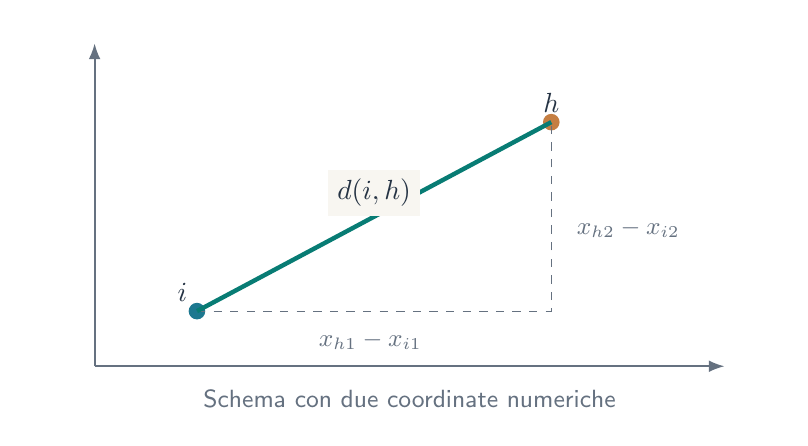
\begin{tikzpicture}[x=1cm,y=1cm]
\path[use as bounding box](-.15,-.15) rectangle(9.4,4.8);
\draw[pAxis](.7,.5)--(8.7,.5);\draw[pAxis](.7,.5)--(.7,4.6);\fill[GeoA](2,1.2) circle(3pt);\fill[GeoB](6.5,3.6) circle(3pt);\node[pLabel,above left] at(2,1.2){$i$};\node[pLabel,above] at(6.5,3.6){$h$};\draw[Muted,dashed](2,1.2)--(6.5,1.2)--(6.5,3.6);\draw[Classical,line width=1.6pt](2,1.2)--(6.5,3.6);\node[pLabel,fill=Paper] at(4.25,2.7){$d(i,h)$};\node[pNote] at(4.2,.82){$x_{h1}-x_{i1}$};\node[pNote,anchor=west] at(6.7,2.25){$x_{h2}-x_{i2}$};\node[pNote] at(4.7,.08){Schema con due coordinate numeriche};
\end{tikzpicture}\PBody{Nel piano, il teorema di Pitagora collega gli scarti lungo due assi alla lunghezza del segmento. La stessa somma si estende a otto coordinate.}
\end{minipage}%
\end{lrbox}
\typeout{FULLBOX:009:L:\the\ht\PilotLeftBox:\the\dp\PilotLeftBox}
\begin{lrbox}{\PilotRightBox}%
\begin{minipage}[t]{7.55cm}\raggedright\color{Ink}\fontsize{11.3}{14.8}\selectfont

\[d(i,h)^2=\sum_{j=1}^{p}(x_{ij}-x_{hj})^2.\]
\PBody{$i$ e $h$ sono due campioni; $p=8$ è il numero delle variabili. Ogni scarto entra al quadrato.}
\PCode{R · calcolare una distanza}{009_distanza.R}
\end{minipage}%
\end{lrbox}
\typeout{FULLBOX:009:R:\the\ht\PilotRightBox:\the\dp\PilotRightBox}
\begin{tikzpicture}[remember picture,overlay]
\PilotChrome{La distanza euclidea combina gli scarti}{I · CAMPIONI, SCALE E DISTANZE}{9}{Prima di interpretare una distanza, occorre conoscere coordinate, unità e trasformazioni.}
\node[anchor=north west,inner sep=0] at([xshift=0.96cm,yshift=-2.13cm]current page.north west){\usebox{\PilotLeftBox}};
\node[anchor=north west,inner sep=0] at([xshift=11.52cm,yshift=-2.13cm]current page.north west){\usebox{\PilotRightBox}};
\end{tikzpicture}\end{frame}

\begin{frame}[plain]\hypertarget{slide10}{}
\bookmark[level=1,page=10]{Centrare e dividere per la dispersione}
\begin{lrbox}{\PilotLeftBox}%
\begin{minipage}[t]{10.05cm}\raggedright\color{Ink}\fontsize{11.3}{14.8}\selectfont
\begin{tikzpicture}[x=1cm,y=1cm]
\path[use as bounding box](-.15,-.15) rectangle(9.4,4.3);

\draw[pAxis](.8,2.6)--(8.7,2.6);
\foreach \x/\t in {1.5/{-2},3.1/{-1},4.7/{0},6.3/{1},7.9/{2}}{\draw[Muted](\x,2.48)--(\x,2.72);\node[pLabel] at(\x,2.1){$\t$};}
\fill[GeoB](6.3,2.6) circle(3.5pt);
\node[pLabel] at(4.7,3.75){$x=\bar x+s\quad\longrightarrow\quad z=1$};
\node[pNote] at(4.7,1.05){Una deviazione standard diventa l’unità di confronto};

\end{tikzpicture}\PBody{Sottrarre la media sposta l’origine. Dividere per la deviazione standard modifica la scala della colonna.}
\end{minipage}%
\end{lrbox}
\typeout{FULLBOX:010:L:\the\ht\PilotLeftBox:\the\dp\PilotLeftBox}
\begin{lrbox}{\PilotRightBox}%
\begin{minipage}[t]{7.55cm}\raggedright\color{Ink}\fontsize{11.3}{14.8}\selectfont

\[z_{ij}=\frac{x_{ij}-\bar x_j}{s_j},\quad s_j>0.\]
\[\bar z_j=0,\qquad s_{z_j}=1.\]
\PBody{La standardizzazione attribuisce lo stesso peso numerico iniziale a uno scarto di una deviazione standard in ciascuna colonna.}
\PInfo{La scelta resta sensibile agli estremi e alla definizione delle variabili. Non rende uguali le forme delle distribuzioni.}

\end{minipage}%
\end{lrbox}
\typeout{FULLBOX:010:R:\the\ht\PilotRightBox:\the\dp\PilotRightBox}
\begin{tikzpicture}[remember picture,overlay]
\PilotChrome{Centrare e dividere per la dispersione}{I · CAMPIONI, SCALE E DISTANZE}{10}{Lo z-score cambia origine e scala; non elimina asimmetria, dipendenza o valori atipici.}
\node[anchor=north west,inner sep=0] at([xshift=0.96cm,yshift=-2.13cm]current page.north west){\usebox{\PilotLeftBox}};
\node[anchor=north west,inner sep=0] at([xshift=11.52cm,yshift=-2.13cm]current page.north west){\usebox{\PilotRightBox}};
\end{tikzpicture}\end{frame}

\begin{frame}[plain]\hypertarget{slide11}{}
\bookmark[level=1,page=11]{Conservare i parametri della standardizzazione}
\begin{lrbox}{\PilotLeftBox}%
\begin{minipage}[t]{10.05cm}\raggedright\color{Ink}\fontsize{11.3}{14.8}\selectfont
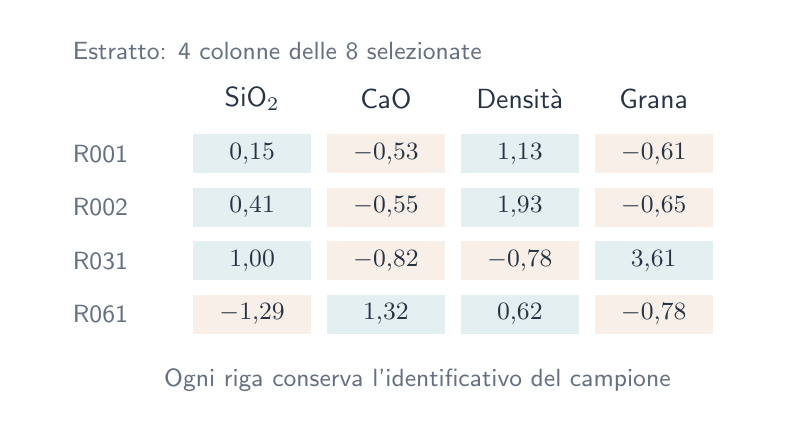
\begin{tikzpicture}[x=1cm,y=1cm]
\path[use as bounding box](-.15,-.15) rectangle(9.4,4.6);
\node[pNote,anchor=west] at(.3,4.3){Estratto: 4 colonne delle 8 selezionate};\node[pLabel] at(2.7,3.7){SiO$_2$};\node[pLabel] at(4.4,3.7){CaO};\node[pLabel] at(6.1,3.7){Densità};\node[pLabel] at(7.8,3.7){Grana};\node[pNote,anchor=west] at(.3,3.0){R001};\fill[GeoA!12](1.95,2.75) rectangle(3.45,3.25);\node[pNote,text=Ink] at(2.7,3.0){$ 0{,}15 $};\fill[GeoB!12](3.65,2.75) rectangle(5.15,3.25);\node[pNote,text=Ink] at(4.4,3.0){$ -0{,}53 $};\fill[GeoA!12](5.35,2.75) rectangle(6.85,3.25);\node[pNote,text=Ink] at(6.1,3.0){$ 1{,}13 $};\fill[GeoB!12](7.05,2.75) rectangle(8.55,3.25);\node[pNote,text=Ink] at(7.8,3.0){$ -0{,}61 $};\node[pNote,anchor=west] at(.3,2.32){R002};\fill[GeoA!12](1.95,2.07) rectangle(3.45,2.57);\node[pNote,text=Ink] at(2.7,2.32){$ 0{,}41 $};\fill[GeoB!12](3.65,2.07) rectangle(5.15,2.57);\node[pNote,text=Ink] at(4.4,2.32){$ -0{,}55 $};\fill[GeoA!12](5.35,2.07) rectangle(6.85,2.57);\node[pNote,text=Ink] at(6.1,2.32){$ 1{,}93 $};\fill[GeoB!12](7.05,2.07) rectangle(8.55,2.57);\node[pNote,text=Ink] at(7.8,2.32){$ -0{,}65 $};\node[pNote,anchor=west] at(.3,1.64){R031};\fill[GeoA!12](1.95,1.39) rectangle(3.45,1.89);\node[pNote,text=Ink] at(2.7,1.64){$ 1{,}00 $};\fill[GeoB!12](3.65,1.39) rectangle(5.15,1.89);\node[pNote,text=Ink] at(4.4,1.64){$ -0{,}82 $};\fill[GeoB!12](5.35,1.39) rectangle(6.85,1.89);\node[pNote,text=Ink] at(6.1,1.64){$ -0{,}78 $};\fill[GeoA!12](7.05,1.39) rectangle(8.55,1.89);\node[pNote,text=Ink] at(7.8,1.64){$ 3{,}61 $};\node[pNote,anchor=west] at(.3,0.96){R061};\fill[GeoB!12](1.95,0.71) rectangle(3.45,1.21);\node[pNote,text=Ink] at(2.7,0.96){$ -1{,}29 $};\fill[GeoA!12](3.65,0.71) rectangle(5.15,1.21);\node[pNote,text=Ink] at(4.4,0.96){$ 1{,}32 $};\fill[GeoA!12](5.35,0.71) rectangle(6.85,1.21);\node[pNote,text=Ink] at(6.1,0.96){$ 0{,}62 $};\fill[GeoB!12](7.05,0.71) rectangle(8.55,1.21);\node[pNote,text=Ink] at(7.8,0.96){$ -0{,}78 $};\node[pNote] at(4.8,.12){Ogni riga conserva l’identificativo del campione};
\end{tikzpicture}\PBody{I numeri standardizzati sono scarti relativi alla variabilità della colonna. Le medie e le scale permettono di ritrovare le unità originali.}
\end{minipage}%
\end{lrbox}
\typeout{FULLBOX:011:L:\the\ht\PilotLeftBox:\the\dp\PilotLeftBox}
\begin{lrbox}{\PilotRightBox}%
\begin{minipage}[t]{7.55cm}\raggedright\color{Ink}\fontsize{11.3}{14.8}\selectfont
\PCode{R · centrare e ridimensionare}{011_standardizzazione.R}\[x_{ij}=\bar x_j+s_jz_{ij}.\]
\end{minipage}%
\end{lrbox}
\typeout{FULLBOX:011:R:\the\ht\PilotRightBox:\the\dp\PilotRightBox}
\begin{tikzpicture}[remember picture,overlay]
\PilotChrome{Conservare i parametri della standardizzazione}{I · CAMPIONI, SCALE E DISTANZE}{11}{Medie, scale e ordine delle colonne fanno parte del risultato dell’analisi.}
\node[anchor=north west,inner sep=0] at([xshift=0.96cm,yshift=-2.13cm]current page.north west){\usebox{\PilotLeftBox}};
\node[anchor=north west,inner sep=0] at([xshift=11.52cm,yshift=-2.13cm]current page.north west){\usebox{\PilotRightBox}};
\end{tikzpicture}\end{frame}

\begin{frame}[plain]\hypertarget{slide12}{}
\bookmark[level=1,page=12]{Collocare un nuovo campione}
\begin{lrbox}{\PilotLeftBox}%
\begin{minipage}[t]{10.05cm}\raggedright\color{Ink}\fontsize{11.3}{14.8}\selectfont
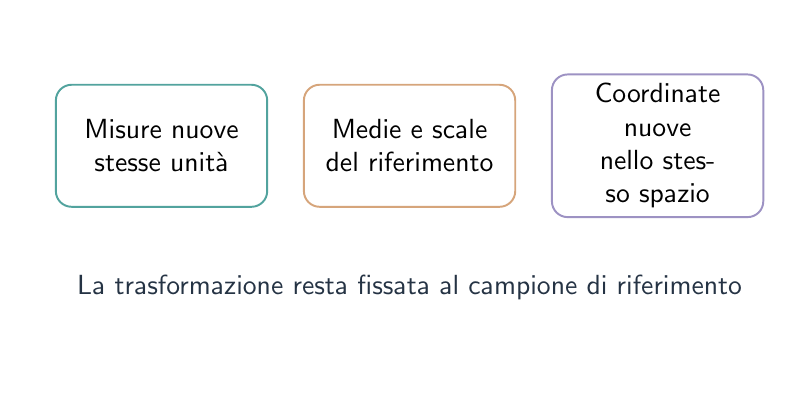
\begin{tikzpicture}[x=1cm,y=1cm]
\path[use as bounding box](-.15,-.15) rectangle(9.4,4.2);
\node[pFlow,draw=Classical!70,text width=2.45cm,minimum height=1.55cm] at(1.55,2.7){Misure nuove\\stesse unità};\node[pFlow,draw=GeoB!70,text width=2.45cm,minimum height=1.55cm] at(4.7,2.7){Medie e scale\\del riferimento};\node[pFlow,draw=GeoC!70,text width=2.45cm,minimum height=1.55cm] at(7.85,2.7){Coordinate nuove\\nello stesso spazio};\node[pLabel,text width=8.6cm] at(4.7,.9){La trasformazione resta fissata al campione di riferimento};
\end{tikzpicture}\PBody{Ricalcolare medie e scale sul nuovo insieme cambierebbe il sistema di coordinate, rendendo incomparabili le posizioni.}
\end{minipage}%
\end{lrbox}
\typeout{FULLBOX:012:L:\the\ht\PilotLeftBox:\the\dp\PilotLeftBox}
\begin{lrbox}{\PilotRightBox}%
\begin{minipage}[t]{7.55cm}\raggedright\color{Ink}\fontsize{11.3}{14.8}\selectfont
\[z_{\mathrm{nuovo},j}=\frac{x_{\mathrm{nuovo},j}-\bar x_j}{s_j}.\]\PCode{R · riutilizzare il riferimento}{012_nuovo_campione.R}
\end{minipage}%
\end{lrbox}
\typeout{FULLBOX:012:R:\the\ht\PilotRightBox:\the\dp\PilotRightBox}
\begin{tikzpicture}[remember picture,overlay]
\PilotChrome{Collocare un nuovo campione}{I · CAMPIONI, SCALE E DISTANZE}{12}{Per confrontare campioni vecchi e nuovi si applica la stessa trasformazione.}
\node[anchor=north west,inner sep=0] at([xshift=0.96cm,yshift=-2.13cm]current page.north west){\usebox{\PilotLeftBox}};
\node[anchor=north west,inner sep=0] at([xshift=11.52cm,yshift=-2.13cm]current page.north west){\usebox{\PilotRightBox}};
\end{tikzpicture}\end{frame}

\begin{frame}[plain]\hypertarget{slide13}{}
\bookmark[level=1,page=13]{Valori mancanti e variabili costanti}
\begin{lrbox}{\PilotLeftBox}%
\begin{minipage}[t]{10.05cm}\raggedright\color{Ink}\fontsize{11.3}{14.8}\selectfont
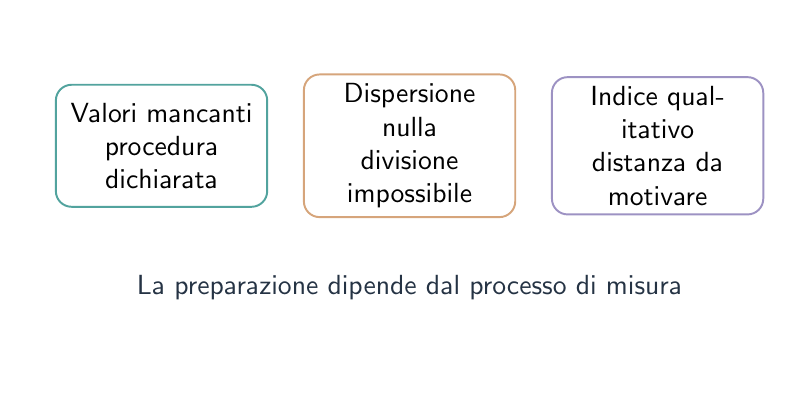
\begin{tikzpicture}[x=1cm,y=1cm]
\path[use as bounding box](-.15,-.15) rectangle(9.4,4.2);
\node[pFlow,draw=Classical!70,text width=2.45cm,minimum height=1.55cm] at(1.55,2.7){Valori mancanti\\procedura dichiarata};\node[pFlow,draw=GeoB!70,text width=2.45cm,minimum height=1.55cm] at(4.7,2.7){Dispersione nulla\\divisione impossibile};\node[pFlow,draw=GeoC!70,text width=2.45cm,minimum height=1.55cm] at(7.85,2.7){Indice qualitativo\\distanza da motivare};\node[pLabel,text width=8.6cm] at(4.7,.9){La preparazione dipende dal processo di misura};
\end{tikzpicture}\PBody{Nel dataset didattico le otto colonne sono complete e variabili. In un rilievo reale, mancanze e limiti analitici richiedono scelte documentate.}
\end{minipage}%
\end{lrbox}
\typeout{FULLBOX:013:L:\the\ht\PilotLeftBox:\the\dp\PilotLeftBox}
\begin{lrbox}{\PilotRightBox}%
\begin{minipage}[t]{7.55cm}\raggedright\color{Ink}\fontsize{11.3}{14.8}\selectfont
\PCode{R · controllare le colonne}{013_controlli.R}\PInfo{Cancellare righe o imputare valori può cambiare distanze e gruppi. La modifica va valutata rispetto alla domanda e alle cause delle mancanze.}
\end{minipage}%
\end{lrbox}
\typeout{FULLBOX:013:R:\the\ht\PilotRightBox:\the\dp\PilotRightBox}
\begin{tikzpicture}[remember picture,overlay]
\PilotChrome{Valori mancanti e variabili costanti}{I · CAMPIONI, SCALE E DISTANZE}{13}{La validità numerica della matrice precede il calcolo; la validità scientifica precede entrambe.}
\node[anchor=north west,inner sep=0] at([xshift=0.96cm,yshift=-2.13cm]current page.north west){\usebox{\PilotLeftBox}};
\node[anchor=north west,inner sep=0] at([xshift=11.52cm,yshift=-2.13cm]current page.north west){\usebox{\PilotRightBox}};
\end{tikzpicture}\end{frame}

\begin{frame}[plain]\hypertarget{slide14}{}
\bookmark[level=1,page=14]{La standardizzazione conserva la correlazione}
\begin{lrbox}{\PilotLeftBox}%
\begin{minipage}[t]{10.05cm}\raggedright\color{Ink}\fontsize{11.3}{14.8}\selectfont
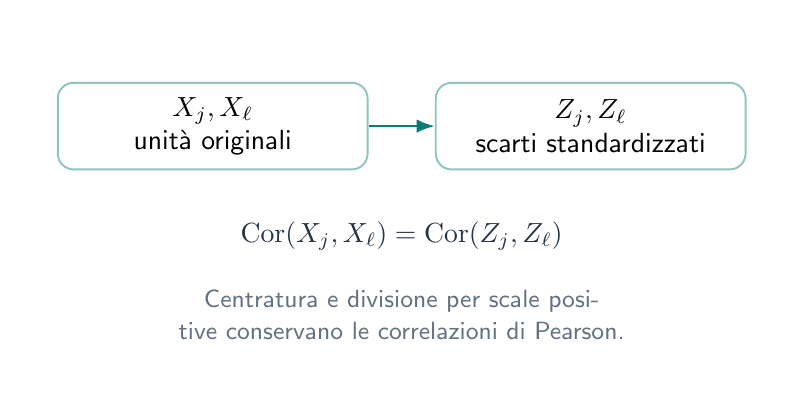
\begin{tikzpicture}[x=1cm,y=1cm]
\path[use as bounding box](-.15,-.15) rectangle(9.4,4.3);

\node[pFlow,text width=3.7cm] (a) at(2.2,3.05){$X_j,X_\ell$\\unità originali};
\node[pFlow,text width=3.7cm] (b) at(7.0,3.05){$Z_j,Z_\ell$\\scarti standardizzati};
\draw[pEdge](a)--(b);
\node[pLabel] at(4.6,1.65){$\operatorname{Cor}(X_j,X_\ell)=\operatorname{Cor}(Z_j,Z_\ell)$};
\node[pNote,text width=8.3cm] at(4.6,.65){Centratura e divisione per scale positive conservano le correlazioni di Pearson.};

\end{tikzpicture}\PBody{Una forte associazione fra due colonne rimane visibile dopo lo z-score. Il problema della ridondanza richiede un esame separato.}
\end{minipage}%
\end{lrbox}
\typeout{FULLBOX:014:L:\the\ht\PilotLeftBox:\the\dp\PilotLeftBox}
\begin{lrbox}{\PilotRightBox}%
\begin{minipage}[t]{7.55cm}\raggedright\color{Ink}\fontsize{11.3}{14.8}\selectfont
\PCode{R · confrontare le correlazioni}{014_correlazioni.R}\PInfo{Media zero e varianza uno non implicano indipendenza. Due colonne standardizzate possono essere quasi identiche.}
\end{minipage}%
\end{lrbox}
\typeout{FULLBOX:014:R:\the\ht\PilotRightBox:\the\dp\PilotRightBox}
\begin{tikzpicture}[remember picture,overlay]
\PilotChrome{La standardizzazione conserva la correlazione}{I · CAMPIONI, SCALE E DISTANZE}{14}{Standardizzazione e rimozione della dipendenza rispondono a problemi diversi.}
\node[anchor=north west,inner sep=0] at([xshift=0.96cm,yshift=-2.13cm]current page.north west){\usebox{\PilotLeftBox}};
\node[anchor=north west,inner sep=0] at([xshift=11.52cm,yshift=-2.13cm]current page.north west){\usebox{\PilotRightBox}};
\end{tikzpicture}\end{frame}

\begin{frame}[plain]\hypertarget{slide15}{}
\bookmark[level=0,page=15]{Ridondanza e composizioni}
\bookmark[level=1,page=15]{Una colonna duplicata pesa due volte}
\begin{lrbox}{\PilotLeftBox}%
\begin{minipage}[t]{10.05cm}\raggedright\color{Ink}\fontsize{11.3}{14.8}\selectfont
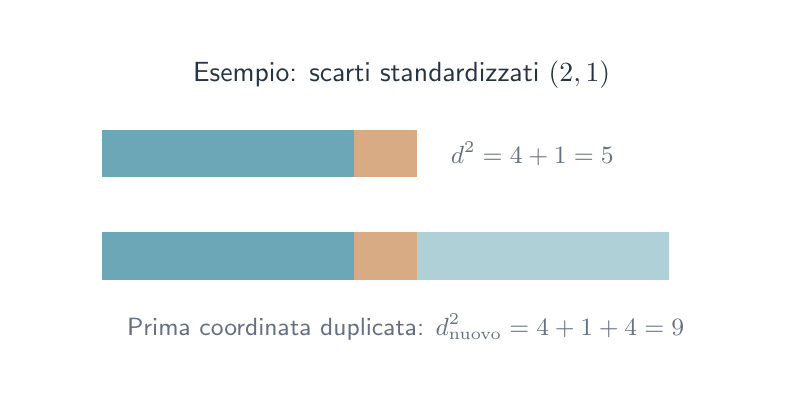
\begin{tikzpicture}[x=1cm,y=1cm]
\path[use as bounding box](-.15,-.15) rectangle(9.4,4.4);

\node[pLabel] at(4.6,3.8){Esempio: scarti standardizzati $(2,1)$};
\fill[GeoA!65](.8,2.5) rectangle(4,3.1);\fill[GeoB!65](4,2.5) rectangle(4.8,3.1);
\node[pNote,anchor=west] at(5.1,2.8){$d^2=4+1=5$};
\fill[GeoA!65](.8,1.2) rectangle(4,1.8);\fill[GeoB!65](4,1.2) rectangle(4.8,1.8);\fill[GeoA!35](4.8,1.2) rectangle(8,1.8);
\node[pNote] at(4.65,.6){Prima coordinata duplicata: $d_{\rm nuovo}^2=4+1+4=9$};

\end{tikzpicture}\PBody{La duplicazione non aggiunge una misura indipendente. Aumenta il peso di una proprietà nella distanza complessiva.}
\end{minipage}%
\end{lrbox}
\typeout{FULLBOX:015:L:\the\ht\PilotLeftBox:\the\dp\PilotLeftBox}
\begin{lrbox}{\PilotRightBox}%
\begin{minipage}[t]{7.55cm}\raggedright\color{Ink}\fontsize{11.3}{14.8}\selectfont
\[d_{\rm nuovo}^2=d^2+(z_{ij}-z_{hj})^2.\]\PCode{R · duplicare una coordinata}{015_duplicazione.R}
\end{minipage}%
\end{lrbox}
\typeout{FULLBOX:015:R:\the\ht\PilotRightBox:\the\dp\PilotRightBox}
\begin{tikzpicture}[remember picture,overlay]
\PilotChrome{Una colonna duplicata pesa due volte}{II · RIDONDANZA E COMPOSIZIONI}{15}{La selezione delle colonne assegna anche pesi impliciti alle proprietà.}
\node[anchor=north west,inner sep=0] at([xshift=0.96cm,yshift=-2.13cm]current page.north west){\usebox{\PilotLeftBox}};
\node[anchor=north west,inner sep=0] at([xshift=11.52cm,yshift=-2.13cm]current page.north west){\usebox{\PilotRightBox}};
\end{tikzpicture}\end{frame}

\begin{frame}[plain]\hypertarget{slide16}{}
\bookmark[level=1,page=16]{I pesi rendono esplicita la scelta}
\begin{lrbox}{\PilotLeftBox}%
\begin{minipage}[t]{10.05cm}\raggedright\color{Ink}\fontsize{11.3}{14.8}\selectfont
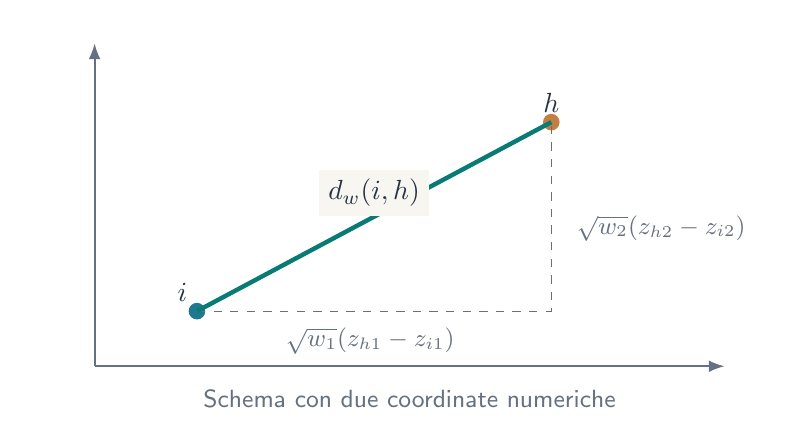
\begin{tikzpicture}[x=1cm,y=1cm]
\path[use as bounding box](-.15,-.15) rectangle(9.4,4.8);
\draw[pAxis](.7,.5)--(8.7,.5);\draw[pAxis](.7,.5)--(.7,4.6);\fill[GeoA](2,1.2) circle(3pt);\fill[GeoB](6.5,3.6) circle(3pt);\node[pLabel,above left] at(2,1.2){$i$};\node[pLabel,above] at(6.5,3.6){$h$};\draw[Muted,dashed](2,1.2)--(6.5,1.2)--(6.5,3.6);\draw[Classical,line width=1.6pt](2,1.2)--(6.5,3.6);\node[pLabel,fill=Paper] at(4.25,2.7){$d_w(i,h)$};\node[pNote] at(4.2,.82){$\sqrt{w_1}(z_{h1}-z_{i1})$};\node[pNote,anchor=west] at(6.7,2.25){$\sqrt{w_2}(z_{h2}-z_{i2})$};\node[pNote] at(4.7,.08){Schema con due coordinate numeriche};
\end{tikzpicture}\PBody{Moltiplicare una coordinata per la radice di un peso equivale a pesare il suo scarto quadratico nella distanza.}
\end{minipage}%
\end{lrbox}
\typeout{FULLBOX:016:L:\the\ht\PilotLeftBox:\the\dp\PilotLeftBox}
\begin{lrbox}{\PilotRightBox}%
\begin{minipage}[t]{7.55cm}\raggedright\color{Ink}\fontsize{11.3}{14.8}\selectfont

\[d_w^2(i,h)=\sum_j w_j(z_{ij}-z_{hj})^2.\]
\PBody{Pesi positivi conservano una distanza euclidea dopo il ridimensionamento. Un peso nullo esclude una direzione dal confronto.}
\PCode{R · applicare pesi dichiarati}{016_pesi.R}
\end{minipage}%
\end{lrbox}
\typeout{FULLBOX:016:R:\the\ht\PilotRightBox:\the\dp\PilotRightBox}
\begin{tikzpicture}[remember picture,overlay]
\PilotChrome{I pesi rendono esplicita la scelta}{II · RIDONDANZA E COMPOSIZIONI}{16}{Un peso va motivato: il calcolo rende la scelta riproducibile, non la giustifica da solo.}
\node[anchor=north west,inner sep=0] at([xshift=0.96cm,yshift=-2.13cm]current page.north west){\usebox{\PilotLeftBox}};
\node[anchor=north west,inner sep=0] at([xshift=11.52cm,yshift=-2.13cm]current page.north west){\usebox{\PilotRightBox}};
\end{tikzpicture}\end{frame}

\begin{frame}[plain]\hypertarget{slide17}{}
\bookmark[level=1,page=17]{Correlazione e ridondanza delle proprietà}
\begin{lrbox}{\PilotLeftBox}%
\begin{minipage}[t]{10.05cm}\raggedright\color{Ink}\fontsize{11.3}{14.8}\selectfont
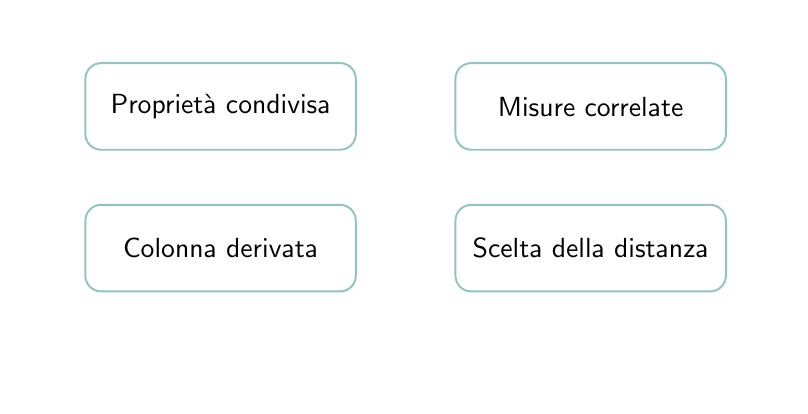
\begin{tikzpicture}[x=1cm,y=1cm]
\path[use as bounding box](-.15,-.15) rectangle(9.4,4.4);
\node[pFlow,text width=3.2cm] at(2.3,3.4){Proprietà condivisa};\node[pFlow,text width=3.2cm] at(7.0,3.4){Misure correlate};\node[pFlow,text width=3.2cm] at(2.3,1.5999999999999999){Colonna derivata};\node[pFlow,text width=3.2cm] at(7.0,1.5999999999999999){Scelta della distanza};
\end{tikzpicture}\PBody{Una correlazione elevata può riflettere un legame fisico, il processo di simulazione, una definizione comune o un vincolo di composizione.}
\end{minipage}%
\end{lrbox}
\typeout{FULLBOX:017:L:\the\ht\PilotLeftBox:\the\dp\PilotLeftBox}
\begin{lrbox}{\PilotRightBox}%
\begin{minipage}[t]{7.55cm}\raggedright\color{Ink}\fontsize{11.3}{14.8}\selectfont
\PCode{R · esaminare la matrice}{017_ridondanza.R}\PInfo{L’esclusione di una misura correlata è una decisione scientifica. Va confrontata con il risultato ottenuto usando entrambe le colonne.}
\end{minipage}%
\end{lrbox}
\typeout{FULLBOX:017:R:\the\ht\PilotRightBox:\the\dp\PilotRightBox}
\begin{tikzpicture}[remember picture,overlay]
\PilotChrome{Correlazione e ridondanza delle proprietà}{II · RIDONDANZA E COMPOSIZIONI}{17}{La ridondanza si interpreta attraverso la definizione delle misure e l’effetto sul risultato.}
\node[anchor=north west,inner sep=0] at([xshift=0.96cm,yshift=-2.13cm]current page.north west){\usebox{\PilotLeftBox}};
\node[anchor=north west,inner sep=0] at([xshift=11.52cm,yshift=-2.13cm]current page.north west){\usebox{\PilotRightBox}};
\end{tikzpicture}\end{frame}

\begin{frame}[plain]\hypertarget{slide18}{}
\bookmark[level=1,page=18]{Una relazione esatta riduce la dimensione}
\begin{lrbox}{\PilotLeftBox}%
\begin{minipage}[t]{10.05cm}\raggedright\color{Ink}\fontsize{11.3}{14.8}\selectfont
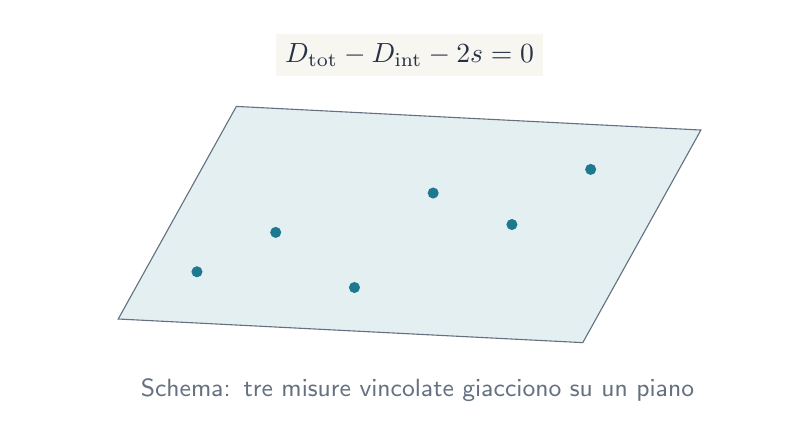
\begin{tikzpicture}[x=1cm,y=1cm]
\path[use as bounding box](-.15,-.15) rectangle(9.4,4.7);

\draw[Muted,fill=GeoA!12](1,1)--(6.9,.7)--(8.4,3.4)--(2.5,3.7)--cycle;
\foreach \x/\y in {2/1.6,3/2.1,4/1.4,5/2.6,6/2.2,7/2.9}{\fill[GeoA](\x,\y) circle(2pt);}
\node[pLabel,fill=Paper] at(4.7,4.35){$D_{\rm tot}-D_{\rm int}-2s=0$};
\node[pNote,text width=8.3cm] at(4.8,.1){Schema: tre misure vincolate giacciono su un piano};

\end{tikzpicture}\PBody{Nel caso dei fossili di Annula, tre colonne derivano da una relazione geometrica. Il terzo asse contiene soltanto l’arrotondamento numerico.}
\end{minipage}%
\end{lrbox}
\typeout{FULLBOX:018:L:\the\ht\PilotLeftBox:\the\dp\PilotLeftBox}
\begin{lrbox}{\PilotRightBox}%
\begin{minipage}[t]{7.55cm}\raggedright\color{Ink}\fontsize{11.3}{14.8}\selectfont
\PCode{R · ritrovare un vincolo noto}{018_fossili.R}\PSmall{Lo scarto massimo è circa $10^{-8}$, coerente con l’arrotondamento delle cifre del CSV.}
\end{minipage}%
\end{lrbox}
\typeout{FULLBOX:018:R:\the\ht\PilotRightBox:\the\dp\PilotRightBox}
\begin{tikzpicture}[remember picture,overlay]
\PilotChrome{Una relazione esatta riduce la dimensione}{II · RIDONDANZA E COMPOSIZIONI}{18}{La dimensione effettiva può essere inferiore al numero delle colonne.}
\node[anchor=north west,inner sep=0] at([xshift=0.96cm,yshift=-2.13cm]current page.north west){\usebox{\PilotLeftBox}};
\node[anchor=north west,inner sep=0] at([xshift=11.52cm,yshift=-2.13cm]current page.north west){\usebox{\PilotRightBox}};
\end{tikzpicture}\end{frame}

\begin{frame}[plain]\hypertarget{slide19}{}
\bookmark[level=1,page=19]{Il rango distingue colonne e informazione}
\begin{lrbox}{\PilotLeftBox}%
\begin{minipage}[t]{10.05cm}\raggedright\color{Ink}\fontsize{11.3}{14.8}\selectfont
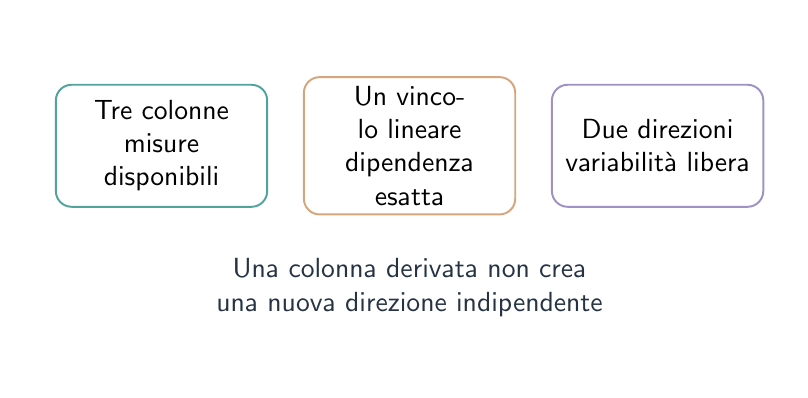
\begin{tikzpicture}[x=1cm,y=1cm]
\path[use as bounding box](-.15,-.15) rectangle(9.4,4.2);
\node[pFlow,draw=Classical!70,text width=2.45cm,minimum height=1.55cm] at(1.55,2.7){Tre colonne\\misure disponibili};\node[pFlow,draw=GeoB!70,text width=2.45cm,minimum height=1.55cm] at(4.7,2.7){Un vincolo lineare\\dipendenza esatta};\node[pFlow,draw=GeoC!70,text width=2.45cm,minimum height=1.55cm] at(7.85,2.7){Due direzioni\\variabilità libera};\node[pLabel,text width=8.6cm] at(4.7,.9){Una colonna derivata non crea una nuova direzione indipendente};
\end{tikzpicture}\PBody{Il rango conta le direzioni linearmente indipendenti. Nei calcoli numerici occorre distinguere uno zero esatto da un valore molto piccolo.}
\end{minipage}%
\end{lrbox}
\typeout{FULLBOX:019:L:\the\ht\PilotLeftBox:\the\dp\PilotLeftBox}
\begin{lrbox}{\PilotRightBox}%
\begin{minipage}[t]{7.55cm}\raggedright\color{Ink}\fontsize{11.3}{14.8}\selectfont

\[\operatorname{rank}(Z)\leq\min(n-1,p).\]
\PBody{La centratura limita il rango a $n-1$. Ulteriori vincoli fra colonne possono ridurlo ancora.}
\PCode{R · valutare la dimensione numerica}{019_rango.R}
\end{minipage}%
\end{lrbox}
\typeout{FULLBOX:019:R:\the\ht\PilotRightBox:\the\dp\PilotRightBox}
\begin{tikzpicture}[remember picture,overlay]
\PilotChrome{Il rango distingue colonne e informazione}{II · RIDONDANZA E COMPOSIZIONI}{19}{Il numero di variabili registrate non coincide necessariamente con la dimensione effettiva.}
\node[anchor=north west,inner sep=0] at([xshift=0.96cm,yshift=-2.13cm]current page.north west){\usebox{\PilotLeftBox}};
\node[anchor=north west,inner sep=0] at([xshift=11.52cm,yshift=-2.13cm]current page.north west){\usebox{\PilotRightBox}};
\end{tikzpicture}\end{frame}

\begin{frame}[plain]\hypertarget{slide20}{}
\bookmark[level=1,page=20]{Le parti di una composizione sono vincolate}
\begin{lrbox}{\PilotLeftBox}%
\begin{minipage}[t]{10.05cm}\raggedright\color{Ink}\fontsize{11.3}{14.8}\selectfont
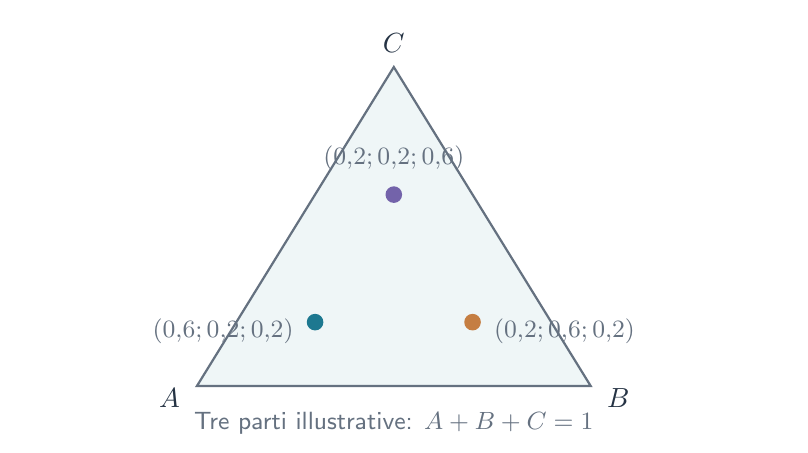
\begin{tikzpicture}[x=1cm,y=1cm]
\path[use as bounding box](-.15,-.15) rectangle(9.4,4.9);
\filldraw[fill=GeoA!7,draw=Muted,line width=.8pt](2,.35)--(7,.35)--(4.5,4.3999999999999995)--cycle;\node[pLabel] at(1.65,.2){$A$};\node[pLabel] at(7.35,.2){$B$};\node[pLabel] at(4.5,4.7){$C$};\fill[GeoA](3.5,1.1600000000000001) circle(3pt);\node[pNote,anchor=east] at(3.35,1.04){$(0{,}6;0{,}2;0{,}2)$};\fill[GeoB](5.500000000000001,1.1600000000000001) circle(3pt);\node[pNote,anchor=west] at(5.650000000000001,1.04){$(0{,}2;0{,}6;0{,}2)$};\fill[GeoC](4.5,2.78) circle(3pt);\node[pNote,anchor=south] at(4.5,2.96){$(0{,}2;0{,}2;0{,}6)$};\node[pNote] at(4.5,-.12){Tre parti illustrative: $A+B+C=1$};
\end{tikzpicture}\PBody{Il triangolo rappresenta tre parti che sommano a uno. Nel dataset, quattro ossidi e il resto completano invece il cento per cento.}
\end{minipage}%
\end{lrbox}
\typeout{FULLBOX:020:L:\the\ht\PilotLeftBox:\the\dp\PilotLeftBox}
\begin{lrbox}{\PilotRightBox}%
\begin{minipage}[t]{7.55cm}\raggedright\color{Ink}\fontsize{11.3}{14.8}\selectfont
\[\sum_{j=1}^{D}x_{ij}=100.\]\PCode{R · verificare la composizione}{020_chiusura.R}\PInfo{La densità e la granulometria non sono parti della composizione chimica. Non entrano nella chiusura.}
\end{minipage}%
\end{lrbox}
\typeout{FULLBOX:020:R:\the\ht\PilotRightBox:\the\dp\PilotRightBox}
\begin{tikzpicture}[remember picture,overlay]
\PilotChrome{Le parti di una composizione sono vincolate}{II · RIDONDANZA E COMPOSIZIONI}{20}{La composizione richiede parti dichiarate e un totale comune; non comprende tutte le colonne numeriche.}
\node[anchor=north west,inner sep=0] at([xshift=0.96cm,yshift=-2.13cm]current page.north west){\usebox{\PilotLeftBox}};
\node[anchor=north west,inner sep=0] at([xshift=11.52cm,yshift=-2.13cm]current page.north west){\usebox{\PilotRightBox}};
\end{tikzpicture}\end{frame}

\begin{frame}[plain]\hypertarget{slide21}{}
\bookmark[level=1,page=21]{La chiusura può indurre associazioni}
\begin{lrbox}{\PilotLeftBox}%
\begin{minipage}[t]{10.05cm}\raggedright\color{Ink}\fontsize{11.3}{14.8}\selectfont
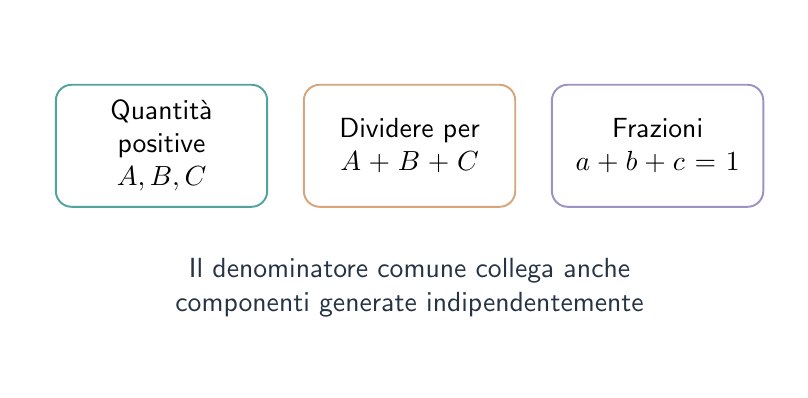
\begin{tikzpicture}[x=1cm,y=1cm]
\path[use as bounding box](-.15,-.15) rectangle(9.4,4.2);
\node[pFlow,draw=Classical!70,text width=2.45cm,minimum height=1.55cm] at(1.55,2.7){Quantità positive\\$A,B,C$};\node[pFlow,draw=GeoB!70,text width=2.45cm,minimum height=1.55cm] at(4.7,2.7){Dividere per\\$A+B+C$};\node[pFlow,draw=GeoC!70,text width=2.45cm,minimum height=1.55cm] at(7.85,2.7){Frazioni\\$a+b+c=1$};\node[pLabel,text width=8.6cm] at(4.7,.9){Il denominatore comune collega anche componenti generate indipendentemente};
\end{tikzpicture}\PBody{La correlazione delle frazioni può differire dalla correlazione delle quantità assolute. Il segno non è fissato universalmente dalla sola chiusura.}
\end{minipage}%
\end{lrbox}
\typeout{FULLBOX:021:L:\the\ht\PilotLeftBox:\the\dp\PilotLeftBox}
\begin{lrbox}{\PilotRightBox}%
\begin{minipage}[t]{7.55cm}\raggedright\color{Ink}\fontsize{11.3}{14.8}\selectfont
\PCode{R · confrontare quantità e frazioni}{021_correlazione_chiusura.R}\PLab{https://marzione00.github.io/Lab_Geo/\#laboratorio/m08-composizioni}{Esperimento · composizioni}
\end{minipage}%
\end{lrbox}
\typeout{FULLBOX:021:R:\the\ht\PilotRightBox:\the\dp\PilotRightBox}
\begin{tikzpicture}[remember picture,overlay]
\PilotChrome{La chiusura può indurre associazioni}{II · RIDONDANZA E COMPOSIZIONI}{21}{Il vincolo sul totale contribuisce alla struttura delle correlazioni osservate.}
\node[anchor=north west,inner sep=0] at([xshift=0.96cm,yshift=-2.13cm]current page.north west){\usebox{\PilotLeftBox}};
\node[anchor=north west,inner sep=0] at([xshift=11.52cm,yshift=-2.13cm]current page.north west){\usebox{\PilotRightBox}};
\end{tikzpicture}\end{frame}

\begin{frame}[plain]\hypertarget{slide22}{}
\bookmark[level=1,page=22]{Un rapporto conserva la scala relativa}
\begin{lrbox}{\PilotLeftBox}%
\begin{minipage}[t]{10.05cm}\raggedright\color{Ink}\fontsize{11.3}{14.8}\selectfont
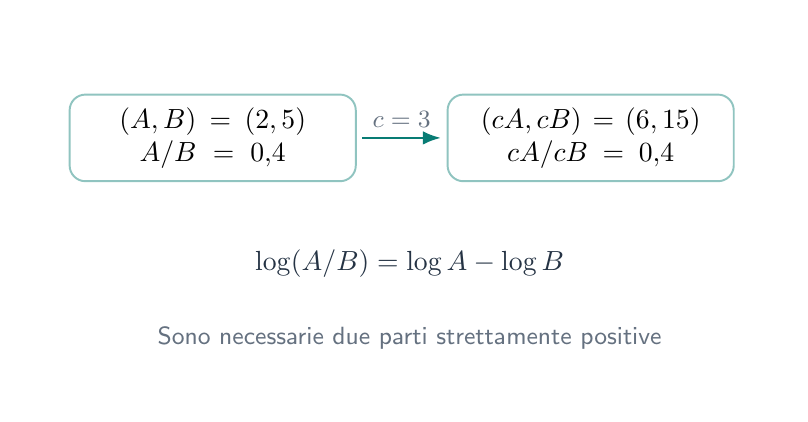
\begin{tikzpicture}[x=1cm,y=1cm]
\path[use as bounding box](-.15,-.15) rectangle(9.4,4.5);

\node[pFlow,text width=3.4cm] at(2.2,3.1){$(A,B)=(2,5)$\\$A/B=0{,}4$};
\node[pFlow,text width=3.4cm] at(7,3.1){$(cA,cB)=(6,15)$\\$cA/cB=0{,}4$};
\draw[pEdge](4.1,3.1)--node[pNote,above]{$c=3$}(5.1,3.1);
\node[pLabel] at(4.7,1.5){$\log(A/B)=\log A-\log B$};
\node[pNote] at(4.7,.55){Sono necessarie due parti strettamente positive};

\end{tikzpicture}\PBody{Moltiplicare tutte le parti per lo stesso fattore non modifica i rapporti. Il logaritmo esprime i rapporti come differenze.}
\end{minipage}%
\end{lrbox}
\typeout{FULLBOX:022:L:\the\ht\PilotLeftBox:\the\dp\PilotLeftBox}
\begin{lrbox}{\PilotRightBox}%
\begin{minipage}[t]{7.55cm}\raggedright\color{Ink}\fontsize{11.3}{14.8}\selectfont
\PCode{R · verificare l’invarianza}{022_rapporti.R}\PInfo{Il log-rapporto rappresenta una relazione fra parti: occorre sapere quali parti vengono confrontate.}
\end{minipage}%
\end{lrbox}
\typeout{FULLBOX:022:R:\the\ht\PilotRightBox:\the\dp\PilotRightBox}
\begin{tikzpicture}[remember picture,overlay]
\PilotChrome{Un rapporto conserva la scala relativa}{II · RIDONDANZA E COMPOSIZIONI}{22}{I rapporti restano invariati alla moltiplicazione comune delle quantità positive.}
\node[anchor=north west,inner sep=0] at([xshift=0.96cm,yshift=-2.13cm]current page.north west){\usebox{\PilotLeftBox}};
\node[anchor=north west,inner sep=0] at([xshift=11.52cm,yshift=-2.13cm]current page.north west){\usebox{\PilotRightBox}};
\end{tikzpicture}\end{frame}

\begin{frame}[plain]\hypertarget{slide23}{}
\bookmark[level=1,page=23]{La trasformazione centrata dei log-rapporti}
\begin{lrbox}{\PilotLeftBox}%
\begin{minipage}[t]{10.05cm}\raggedright\color{Ink}\fontsize{11.3}{14.8}\selectfont
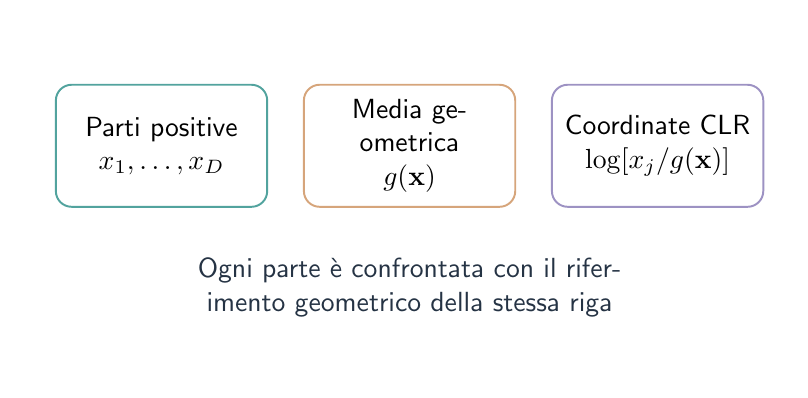
\begin{tikzpicture}[x=1cm,y=1cm]
\path[use as bounding box](-.15,-.15) rectangle(9.4,4.2);
\node[pFlow,draw=Classical!70,text width=2.45cm,minimum height=1.55cm] at(1.55,2.7){Parti positive\\$x_1,\ldots,x_D$};\node[pFlow,draw=GeoB!70,text width=2.45cm,minimum height=1.55cm] at(4.7,2.7){Media geometrica\\$g(\mathbf x)$};\node[pFlow,draw=GeoC!70,text width=2.45cm,minimum height=1.55cm] at(7.85,2.7){Coordinate CLR\\$\log[x_j/g(\mathbf x)]$};\node[pLabel,text width=8.6cm] at(4.7,.9){Ogni parte è confrontata con il riferimento geometrico della stessa riga};
\end{tikzpicture}\[g(\mathbf x)=\exp\!\left(\frac1D\sum_j\log x_j\right).\]
\end{minipage}%
\end{lrbox}
\typeout{FULLBOX:023:L:\the\ht\PilotLeftBox:\the\dp\PilotLeftBox}
\begin{lrbox}{\PilotRightBox}%
\begin{minipage}[t]{7.55cm}\raggedright\color{Ink}\fontsize{11.3}{14.8}\selectfont
\[\operatorname{clr}(\mathbf x)_j=\log x_j-\frac1D\sum_\ell\log x_\ell.\]\PCode{R · calcolare le coordinate CLR}{023_clr.R}
\end{minipage}%
\end{lrbox}
\typeout{FULLBOX:023:R:\the\ht\PilotRightBox:\the\dp\PilotRightBox}
\begin{tikzpicture}[remember picture,overlay]
\PilotChrome{La trasformazione centrata dei log-rapporti}{II · RIDONDANZA E COMPOSIZIONI}{23}{La CLR descrive ogni parte rispetto alla media geometrica; non standardizza le otto proprietà miste.}
\node[anchor=north west,inner sep=0] at([xshift=0.96cm,yshift=-2.13cm]current page.north west){\usebox{\PilotLeftBox}};
\node[anchor=north west,inner sep=0] at([xshift=11.52cm,yshift=-2.13cm]current page.north west){\usebox{\PilotRightBox}};
\end{tikzpicture}\end{frame}

\begin{frame}[plain]\hypertarget{slide24}{}
\bookmark[level=1,page=24]{Le coordinate CLR sommano a zero}
\begin{lrbox}{\PilotLeftBox}%
\begin{minipage}[t]{10.05cm}\raggedright\color{Ink}\fontsize{11.3}{14.8}\selectfont
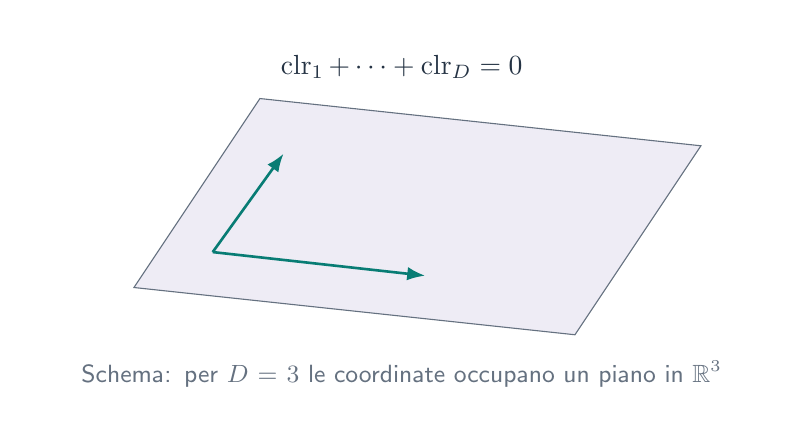
\begin{tikzpicture}[x=1cm,y=1cm]
\path[use as bounding box](-.15,-.15) rectangle(9.4,4.5);

\node[pLabel] at(4.6,4){$\operatorname{clr}_1+\cdots+\operatorname{clr}_D=0$};
\draw[Muted,fill=GeoC!12](1.2,1.2)--(6.8,.6)--(8.4,3)--(2.8,3.6)--cycle;
\draw[pEdge](2.2,1.65)--(4.9,1.35);\draw[pEdge](2.2,1.65)--(3.1,2.9);
\node[pNote,text width=8.5cm] at(4.6,.1){Schema: per $D=3$ le coordinate occupano un piano in $\mathbb R^3$};

\end{tikzpicture}\PBody{Cinque coordinate CLR appartengono a uno spazio di dimensione al più quattro. La covarianza è singolare per costruzione.}
\end{minipage}%
\end{lrbox}
\typeout{FULLBOX:024:L:\the\ht\PilotLeftBox:\the\dp\PilotLeftBox}
\begin{lrbox}{\PilotRightBox}%
\begin{minipage}[t]{7.55cm}\raggedright\color{Ink}\fontsize{11.3}{14.8}\selectfont
\[\operatorname{rank}\{\operatorname{Cov}(\mathrm{CLR})\}\leq D-1.\]\PCode{R · riconoscere la singolarità}{024_pca_clr.R}\PSmall{Qui la scala CLR viene mantenuta. Ridimensionare separatamente le sue colonne cambierebbe la geometria.}
\end{minipage}%
\end{lrbox}
\typeout{FULLBOX:024:R:\the\ht\PilotRightBox:\the\dp\PilotRightBox}
\begin{tikzpicture}[remember picture,overlay]
\PilotChrome{Le coordinate CLR sommano a zero}{II · RIDONDANZA E COMPOSIZIONI}{24}{Una covarianza singolare può derivare da un vincolo scientifico noto, non da un errore del software.}
\node[anchor=north west,inner sep=0] at([xshift=0.96cm,yshift=-2.13cm]current page.north west){\usebox{\PilotLeftBox}};
\node[anchor=north west,inner sep=0] at([xshift=11.52cm,yshift=-2.13cm]current page.north west){\usebox{\PilotRightBox}};
\end{tikzpicture}\end{frame}

\begin{frame}[plain]\hypertarget{slide25}{}
\bookmark[level=1,page=25]{Gli zeri richiedono una spiegazione}
\begin{lrbox}{\PilotLeftBox}%
\begin{minipage}[t]{10.05cm}\raggedright\color{Ink}\fontsize{11.3}{14.8}\selectfont
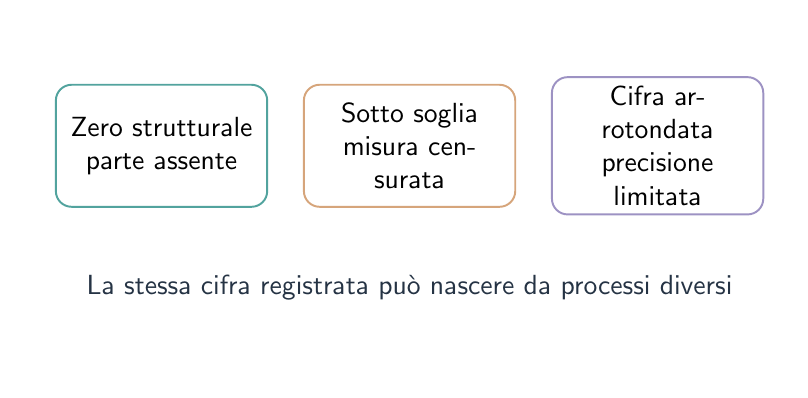
\begin{tikzpicture}[x=1cm,y=1cm]
\path[use as bounding box](-.15,-.15) rectangle(9.4,4.2);
\node[pFlow,draw=Classical!70,text width=2.45cm,minimum height=1.55cm] at(1.55,2.7){Zero strutturale\\parte assente};\node[pFlow,draw=GeoB!70,text width=2.45cm,minimum height=1.55cm] at(4.7,2.7){Sotto soglia\\misura censurata};\node[pFlow,draw=GeoC!70,text width=2.45cm,minimum height=1.55cm] at(7.85,2.7){Cifra arrotondata\\precisione limitata};\node[pLabel,text width=8.6cm] at(4.7,.9){La stessa cifra registrata può nascere da processi diversi};
\end{tikzpicture}\PBody{Il logaritmo di zero non è definito. Aggiungere una costante cambia soprattutto i rapporti che coinvolgono parti poco abbondanti.}
\end{minipage}%
\end{lrbox}
\typeout{FULLBOX:025:L:\the\ht\PilotLeftBox:\the\dp\PilotLeftBox}
\begin{lrbox}{\PilotRightBox}%
\begin{minipage}[t]{7.55cm}\raggedright\color{Ink}\fontsize{11.3}{14.8}\selectfont

\[\log\frac{x_j+\delta}{x_\ell+\delta}\not\equiv\log\frac{x_j}{x_\ell}.\]
\PBody{Il parametro $\delta$ introduce una scelta aggiuntiva. Deve essere collegato al processo di misura e valutato con un’analisi di sensibilità.}
\PInfo{Le cinque parti chimiche del dataset sono positive. Gli zeri presenti in altri indici non autorizzano a includerli nella composizione.}

\end{minipage}%
\end{lrbox}
\typeout{FULLBOX:025:R:\the\ht\PilotRightBox:\the\dp\PilotRightBox}
\begin{tikzpicture}[remember picture,overlay]
\PilotChrome{Gli zeri richiedono una spiegazione}{II · RIDONDANZA E COMPOSIZIONI}{25}{Prima di sostituire uno zero, occorre distinguere assenza reale, censura e arrotondamento.}
\node[anchor=north west,inner sep=0] at([xshift=0.96cm,yshift=-2.13cm]current page.north west){\usebox{\PilotLeftBox}};
\node[anchor=north west,inner sep=0] at([xshift=11.52cm,yshift=-2.13cm]current page.north west){\usebox{\PilotRightBox}};
\end{tikzpicture}\end{frame}

\begin{frame}[plain]\hypertarget{slide26}{}
\bookmark[level=1,page=26]{Due geometrie per due domande}
\begin{lrbox}{\PilotLeftBox}%
\begin{minipage}[t]{10.05cm}\raggedright\color{Ink}\fontsize{11.3}{14.8}\selectfont
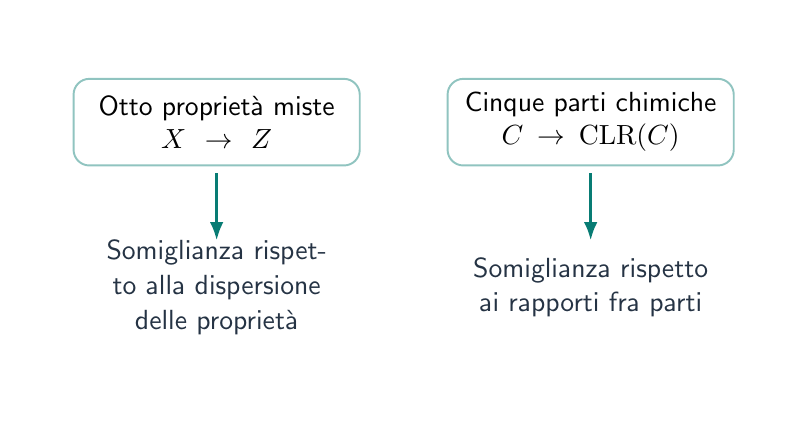
\begin{tikzpicture}[x=1cm,y=1cm]
\path[use as bounding box](-.15,-.15) rectangle(9.4,4.5);

\node[pFlow,text width=3.4cm] at(2.25,3.3){Otto proprietà miste\\$X\to Z$};
\node[pFlow,text width=3.4cm] at(7.0,3.3){Cinque parti chimiche\\$C\to\mathrm{CLR}(C)$};
\draw[pEdge](2.25,2.65)--(2.25,1.8);\draw[pEdge](7,2.65)--(7,1.8);
\node[pLabel,text width=3.7cm] at(2.25,1.2){Somiglianza rispetto alla dispersione delle proprietà};
\node[pLabel,text width=3.7cm] at(7,1.2){Somiglianza rispetto ai rapporti fra parti};

\end{tikzpicture}\PBody{Il percorso principale usa le otto proprietà standardizzate del laboratorio. L’approfondimento CLR risponde a una domanda composizionale distinta.}
\end{minipage}%
\end{lrbox}
\typeout{FULLBOX:026:L:\the\ht\PilotLeftBox:\the\dp\PilotLeftBox}
\begin{lrbox}{\PilotRightBox}%
\begin{minipage}[t]{7.55cm}\raggedright\color{Ink}\fontsize{11.3}{14.8}\selectfont

\PLabel{Scelte da documentare}
\PBody{Variabili incluse, trasformazione, unità, eventuali pesi e trattamento delle misure mancanti.}
\vspace{4mm}
\PInfo{Le due rappresentazioni non si confrontano soltanto contando quanti gruppi producono. Cambiano le proprietà considerate e il significato della distanza.}
\vspace{3mm}
\PBody{La PCA viene ora costruita sulla matrice $Z$ delle otto variabili.}

\end{minipage}%
\end{lrbox}
\typeout{FULLBOX:026:R:\the\ht\PilotRightBox:\the\dp\PilotRightBox}
\begin{tikzpicture}[remember picture,overlay]
\PilotChrome{Due geometrie per due domande}{II · RIDONDANZA E COMPOSIZIONI}{26}{La geometria dell’analisi deve corrispondere alla domanda sulle somiglianze dei campioni.}
\node[anchor=north west,inner sep=0] at([xshift=0.96cm,yshift=-2.13cm]current page.north west){\usebox{\PilotLeftBox}};
\node[anchor=north west,inner sep=0] at([xshift=11.52cm,yshift=-2.13cm]current page.north west){\usebox{\PilotRightBox}};
\end{tikzpicture}\end{frame}

\begin{frame}[plain]\hypertarget{slide27}{}
\bookmark[level=0,page=27]{Geometria della PCA}
\bookmark[level=1,page=27]{La nuvola dei campioni ha direzioni privilegiate}
\begin{lrbox}{\PilotLeftBox}%
\begin{minipage}[t]{10.05cm}\raggedright\color{Ink}\fontsize{11.3}{14.8}\selectfont
\begin{tikzpicture}[x=1cm,y=1cm]
\path[use as bounding box](-.15,-.2) rectangle(9.1,4.800000000000001);
\draw[pAxis](2.3,0.7)--(7.170000000000001,0.7);
\draw[pAxis](2.3,0.7)--(2.3,4.32);
\draw[Muted](2.8000,0.6499999999999999)--(2.8000,0.75);\node[pNote] at(2.8000,0.44999999999999996){$ -3 $};
\draw[Muted](4.6750,0.6499999999999999)--(4.6750,0.75);\node[pNote] at(4.6750,0.44999999999999996){$ 0 $};
\draw[Muted](6.5500,0.6499999999999999)--(6.5500,0.75);\node[pNote] at(6.5500,0.44999999999999996){$ 3 $};
\draw[Muted](2.25,1.2000)--(2.3499999999999996,1.2000);\node[pNote,anchor=east] at(2.1999999999999997,1.2000){$ -2 $};
\draw[Muted](2.25,2.4500)--(2.3499999999999996,2.4500);\node[pNote,anchor=east] at(2.1999999999999997,2.4500){$ 0 $};
\draw[Muted](2.25,3.7000)--(2.3499999999999996,3.7000);\node[pNote,anchor=east] at(2.1999999999999997,3.7000){$ 2 $};
\node[pNote] at(4.675000000000001,0.12){$z_1$};
\node[pNote,rotate=90] at(1.65,2.45){$z_2$};
\fill[GeoA](2.8000,1.4732) circle(1.6pt);
\fill[GeoA](2.9875,1.1072) circle(1.6pt);
\fill[GeoA](3.1750,1.4789) circle(1.6pt);
\fill[GeoA](3.3625,1.8364) circle(1.6pt);
\fill[GeoA](3.5500,1.4705) circle(1.6pt);
\fill[GeoA](3.7375,1.8493) circle(1.6pt);
\fill[GeoA](3.9250,2.1996) circle(1.6pt);
\fill[GeoA](4.1125,1.8339) circle(1.6pt);
\fill[GeoA](4.3000,2.2196) circle(1.6pt);
\fill[GeoA](4.4875,2.5626) circle(1.6pt);
\fill[GeoA](4.6750,2.1974) circle(1.6pt);
\fill[GeoA](4.8625,2.5900) circle(1.6pt);
\fill[GeoA](5.0500,2.9256) circle(1.6pt);
\fill[GeoA](5.2375,2.5610) circle(1.6pt);
\fill[GeoA](5.4250,2.9603) circle(1.6pt);
\fill[GeoA](5.6125,3.2886) circle(1.6pt);
\fill[GeoA](5.8000,2.9246) circle(1.6pt);
\fill[GeoA](5.9875,3.3306) circle(1.6pt);
\fill[GeoA](6.1750,3.6514) circle(1.6pt);
\fill[GeoA](6.3625,3.2883) circle(1.6pt);
\fill[GeoA](6.5500,3.7010) circle(1.6pt);
\end{tikzpicture}\PBody{Esempio didattico con due variabili centrate: i punti occupano una fascia inclinata. Una direzione lungo la fascia ne conserva gran parte della variabilità.}
\end{minipage}%
\end{lrbox}
\typeout{FULLBOX:027:L:\the\ht\PilotLeftBox:\the\dp\PilotLeftBox}
\begin{lrbox}{\PilotRightBox}%
\begin{minipage}[t]{7.55cm}\raggedright\color{Ink}\fontsize{11.3}{14.8}\selectfont

\PLabel{Rappresentare con meno coordinate}
\PBody{La PCA cerca assi nuovi attraverso il centro della nuvola. La prima direzione massimizza la varianza delle coordinate proiettate.}
\vspace{4mm}
\PInfo{La PCA considera congiuntamente le variabili selezionate. Non richiede una risposta da prevedere.}
\vspace{3mm}
\[\mathbf z_i\in\mathbb R^p\quad\longmapsto\quad t_i\in\mathbb R.\]

\end{minipage}%
\end{lrbox}
\typeout{FULLBOX:027:R:\the\ht\PilotRightBox:\the\dp\PilotRightBox}
\begin{tikzpicture}[remember picture,overlay]
\PilotChrome{La nuvola dei campioni ha direzioni privilegiate}{III · GEOMETRIA DELLA PCA}{27}{Una componente principale è una coordinata costruita dalle variabili della matrice centrata.}
\node[anchor=north west,inner sep=0] at([xshift=0.96cm,yshift=-2.13cm]current page.north west){\usebox{\PilotLeftBox}};
\node[anchor=north west,inner sep=0] at([xshift=11.52cm,yshift=-2.13cm]current page.north west){\usebox{\PilotRightBox}};
\end{tikzpicture}\end{frame}

\begin{frame}[plain]\hypertarget{slide28}{}
\bookmark[level=1,page=28]{Il prodotto scalare dà una coordinata}
\begin{lrbox}{\PilotLeftBox}%
\begin{minipage}[t]{10.05cm}\raggedright\color{Ink}\fontsize{11.3}{14.8}\selectfont
\begin{tikzpicture}[x=1cm,y=1cm]
\path[use as bounding box](-.15,-.2) rectangle(9.1,4.800000000000001);
\draw[pAxis](2.3865384615384615,0.7)--(7.083461538461539,0.7);
\draw[pAxis](2.3865384615384615,0.7)--(2.3865384615384615,4.32);
\draw[Muted](2.9250,0.6499999999999999)--(2.9250,0.75);\node[pNote] at(2.9250,0.44999999999999996){$ 0 $};
\draw[Muted](4.2712,0.6499999999999999)--(4.2712,0.75);\node[pNote] at(4.2712,0.44999999999999996){$ 1 $};
\draw[Muted](5.6173,0.6499999999999999)--(5.6173,0.75);\node[pNote] at(5.6173,0.44999999999999996){$ 2 $};
\draw[Muted](6.9635,0.6499999999999999)--(6.9635,0.75);\node[pNote] at(6.9635,0.44999999999999996){$ 3 $};
\draw[Muted](2.3365384615384617,1.2385)--(2.4365384615384613,1.2385);\node[pNote,anchor=east] at(2.2865384615384614,1.2385){$ 0 $};
\draw[Muted](2.3365384615384617,2.5846)--(2.4365384615384613,2.5846);\node[pNote,anchor=east] at(2.2865384615384614,2.5846){$ 1 $};
\draw[Muted](2.3365384615384617,3.9308)--(2.4365384615384613,3.9308);\node[pNote,anchor=east] at(2.2865384615384614,3.9308){$ 2 $};
\node[pNote] at(4.675000000000001,0.12){$z_1$};
\node[pNote,rotate=90] at(1.7365384615384616,2.45){$z_2$};
\draw[Classical,line width=1pt] plot coordinates {(2.3865,0.8346) (6.5596,3.9644)};
\draw[GeoA,-{Latex},line width=1.2pt] plot coordinates {(2.9250,1.2385) (5.6173,2.5846)};
\draw[Classical,-{Latex},line width=1.4pt] plot coordinates {(2.9250,1.2385) (5.2942,3.0154)};
\draw[GeoB,dashed,line width=1.2pt] plot coordinates {(5.2942,3.0154) (5.6173,2.5846)};
\fill[GeoA](5.617,2.585) circle(2.8pt);\node[pLabel,anchor=north west] at(5.717,2.505){$\mathbf z=(2,1)$};
\node[pNote,anchor=south east] at(5.194,3.115){$\widehat{\mathbf z}=(1{,}76;1{,}32)$};
\end{tikzpicture}\PBody{Il vettore unitario $\mathbf v=(0{,}8;0{,}6)$ fissa una direzione. Il prodotto scalare misura la coordinata di $\mathbf z$ lungo quella direzione.}
\end{minipage}%
\end{lrbox}
\typeout{FULLBOX:028:L:\the\ht\PilotLeftBox:\the\dp\PilotLeftBox}
\begin{lrbox}{\PilotRightBox}%
\begin{minipage}[t]{7.55cm}\raggedright\color{Ink}\fontsize{11.3}{14.8}\selectfont

\[t=\mathbf z^\top\mathbf v.\]
\[t=2(0{,}8)+1(0{,}6)=2{,}2.\]
\PCode{R · calcolare uno score}{028_prodotto_scalare.R}\PSmall{Il simbolo $t$ indica una coordinata scalare, non un vettore nel piano.}
\end{minipage}%
\end{lrbox}
\typeout{FULLBOX:028:R:\the\ht\PilotRightBox:\the\dp\PilotRightBox}
\begin{tikzpicture}[remember picture,overlay]
\PilotChrome{Il prodotto scalare dà una coordinata}{III · GEOMETRIA DELLA PCA}{28}{Lo score è il prodotto scalare fra la riga centrata e una direzione unitaria.}
\node[anchor=north west,inner sep=0] at([xshift=0.96cm,yshift=-2.13cm]current page.north west){\usebox{\PilotLeftBox}};
\node[anchor=north west,inner sep=0] at([xshift=11.52cm,yshift=-2.13cm]current page.north west){\usebox{\PilotRightBox}};
\end{tikzpicture}\end{frame}

\begin{frame}[plain]\hypertarget{slide29}{}
\bookmark[level=1,page=29]{La proiezione torna nello spazio delle misure}
\begin{lrbox}{\PilotLeftBox}%
\begin{minipage}[t]{10.05cm}\raggedright\color{Ink}\fontsize{11.3}{14.8}\selectfont
\begin{tikzpicture}[x=1cm,y=1cm]
\path[use as bounding box](-.15,-.2) rectangle(9.1,4.800000000000001);
\draw[pAxis](2.3865384615384615,0.7)--(7.083461538461539,0.7);
\draw[pAxis](2.3865384615384615,0.7)--(2.3865384615384615,4.32);
\draw[Muted](2.9250,0.6499999999999999)--(2.9250,0.75);\node[pNote] at(2.9250,0.44999999999999996){$ 0 $};
\draw[Muted](4.2712,0.6499999999999999)--(4.2712,0.75);\node[pNote] at(4.2712,0.44999999999999996){$ 1 $};
\draw[Muted](5.6173,0.6499999999999999)--(5.6173,0.75);\node[pNote] at(5.6173,0.44999999999999996){$ 2 $};
\draw[Muted](6.9635,0.6499999999999999)--(6.9635,0.75);\node[pNote] at(6.9635,0.44999999999999996){$ 3 $};
\draw[Muted](2.3365384615384617,1.2385)--(2.4365384615384613,1.2385);\node[pNote,anchor=east] at(2.2865384615384614,1.2385){$ 0 $};
\draw[Muted](2.3365384615384617,2.5846)--(2.4365384615384613,2.5846);\node[pNote,anchor=east] at(2.2865384615384614,2.5846){$ 1 $};
\draw[Muted](2.3365384615384617,3.9308)--(2.4365384615384613,3.9308);\node[pNote,anchor=east] at(2.2865384615384614,3.9308){$ 2 $};
\node[pNote] at(4.675000000000001,0.12){$z_1$};
\node[pNote,rotate=90] at(1.7365384615384616,2.45){$z_2$};
\draw[Classical,line width=1pt] plot coordinates {(2.3865,0.8346) (6.5596,3.9644)};
\draw[GeoA,-{Latex},line width=1.2pt] plot coordinates {(2.9250,1.2385) (5.6173,2.5846)};
\draw[Classical,-{Latex},line width=1.4pt] plot coordinates {(2.9250,1.2385) (5.2942,3.0154)};
\draw[GeoB,dashed,line width=1.2pt] plot coordinates {(5.2942,3.0154) (5.6173,2.5846)};
\fill[GeoA](5.617,2.585) circle(2.8pt);\node[pLabel,anchor=north west] at(5.717,2.505){$\mathbf z=(2,1)$};
\node[pNote,anchor=south east] at(5.194,3.115){$\widehat{\mathbf z}=(1{,}76;1{,}32)$};
\end{tikzpicture}\PBody{Moltiplicando lo score per la direzione si ricostruisce la proiezione. Lo scarto residuo è ortogonale all’asse.}
\end{minipage}%
\end{lrbox}
\typeout{FULLBOX:029:L:\the\ht\PilotLeftBox:\the\dp\PilotLeftBox}
\begin{lrbox}{\PilotRightBox}%
\begin{minipage}[t]{7.55cm}\raggedright\color{Ink}\fontsize{11.3}{14.8}\selectfont
\[\widehat{\mathbf z}=t\mathbf v,\qquad \mathbf r=\mathbf z-t\mathbf v.\]\PCode{R · controllare l’ortogonalità}{029_proiezione.R}\PInfo{Nel diagramma: $\widehat{\mathbf z}=(1{,}76;1{,}32)$ e $\mathbf r=(0{,}24;-0{,}32)$.}
\end{minipage}%
\end{lrbox}
\typeout{FULLBOX:029:R:\the\ht\PilotRightBox:\the\dp\PilotRightBox}
\begin{tikzpicture}[remember picture,overlay]
\PilotChrome{La proiezione torna nello spazio delle misure}{III · GEOMETRIA DELLA PCA}{29}{La proiezione è un vettore; lo score ne è la coordinata sull’asse scelto.}
\node[anchor=north west,inner sep=0] at([xshift=0.96cm,yshift=-2.13cm]current page.north west){\usebox{\PilotLeftBox}};
\node[anchor=north west,inner sep=0] at([xshift=11.52cm,yshift=-2.13cm]current page.north west){\usebox{\PilotRightBox}};
\end{tikzpicture}\end{frame}

\begin{frame}[plain]\hypertarget{slide30}{}
\bookmark[level=1,page=30]{Ruotare l’asse cambia la varianza}
\begin{lrbox}{\PilotLeftBox}%
\begin{minipage}[t]{10.05cm}\raggedright\color{Ink}\fontsize{11.3}{14.8}\selectfont
\begin{tikzpicture}[x=1cm,y=1cm]
\path[use as bounding box](-.15,-.2) rectangle(9.1,4.75);
\draw[pAxis](0.8,0.7)--(8.67,0.7);
\draw[pAxis](0.8,0.7)--(0.8,4.27);
\draw[Muted](0.8000,0.6499999999999999)--(0.8000,0.75);\node[pNote] at(0.8000,0.44999999999999996){$ 0 $};
\draw[Muted](2.7375,0.6499999999999999)--(2.7375,0.75);\node[pNote] at(2.7375,0.44999999999999996){$ 45 $};
\draw[Muted](4.6750,0.6499999999999999)--(4.6750,0.75);\node[pNote] at(4.6750,0.44999999999999996){$ 90 $};
\draw[Muted](6.6125,0.6499999999999999)--(6.6125,0.75);\node[pNote] at(6.6125,0.44999999999999996){$ 135 $};
\draw[Muted](8.5500,0.6499999999999999)--(8.5500,0.75);\node[pNote] at(8.5500,0.44999999999999996){$ 180 $};
\draw[Muted](0.75,0.7000)--(0.8500000000000001,0.7000);\node[pNote,anchor=east] at(0.7000000000000001,0.7000){$ 0 $};
\draw[Muted](0.75,2.0800)--(0.8500000000000001,2.0800);\node[pNote,anchor=east] at(0.7000000000000001,2.0800){$ 2 $};
\draw[Muted](0.75,3.4600)--(0.8500000000000001,3.4600);\node[pNote,anchor=east] at(0.7000000000000001,3.4600){$ 4 $};
\node[pNote] at(4.675,0.12){Angolo $\theta$ (gradi)};
\node[pNote,rotate=90] at(0.15000000000000002,2.425){Varianza proiettata};
\draw[Classical,line width=1.1pt] plot coordinates {(0.8000,3.0908) (0.8861,3.1959) (0.9722,3.2971) (1.0583,3.3941) (1.1444,3.4864) (1.2306,3.5734) (1.3167,3.6548) (1.4028,3.7303) (1.4889,3.7993) (1.5750,3.8617) (1.6611,3.9170) (1.7472,3.9650) (1.8333,4.0055) (1.9194,4.0383) (2.0056,4.0632) (2.0917,4.0801) (2.1778,4.0889) (2.2639,4.0896) (2.3500,4.0822) (2.4361,4.0667) (2.5222,4.0431) (2.6083,4.0117) (2.6944,3.9725) (2.7806,3.9257) (2.8667,3.8717) (2.9528,3.8105) (3.0389,3.7426) (3.1250,3.6682) (3.2111,3.5878) (3.2972,3.5017) (3.3833,3.4103) (3.4694,3.3141) (3.5556,3.2135) (3.6417,3.1091) (3.7278,3.0013) (3.8139,2.8908) (3.9000,2.7779) (3.9861,2.6632) (4.0722,2.5474) (4.1583,2.4310) (4.2444,2.3146) (4.3306,2.1986) (4.4167,2.0838) (4.5028,1.9705) (4.5889,1.8595) (4.6750,1.7512) (4.7611,1.6462) (4.8472,1.5449) (4.9333,1.4480) (5.0194,1.3557) (5.1056,1.2687) (5.1917,1.1872) (5.2778,1.1118) (5.3639,1.0427) (5.4500,0.9804) (5.5361,0.9251) (5.6222,0.8771) (5.7083,0.8366) (5.7944,0.8038) (5.8806,0.7789) (5.9667,0.7620) (6.0528,0.7531) (6.1389,0.7524) (6.2250,0.7599) (6.3111,0.7754) (6.3972,0.7989) (6.4833,0.8304) (6.5694,0.8696) (6.6556,0.9163) (6.7417,0.9704) (6.8278,1.0316) (6.9139,1.0995) (7.0000,1.1738) (7.0861,1.2543) (7.1722,1.3404) (7.2583,1.4318) (7.3444,1.5280) (7.4306,1.6285) (7.5167,1.7330) (7.6028,1.8407) (7.6889,1.9513) (7.7750,2.0642) (7.8611,2.1788) (7.9472,2.2946) (8.0333,2.4110) (8.1194,2.5275) (8.2056,2.6435) (8.2917,2.7583) (8.3778,2.8715) (8.4639,2.9826) (8.5500,3.0908)};
\draw[GeoB,dashed] plot coordinates {(2.2282,0.7000) (2.2282,4.0903)};
\fill[GeoB](2.2282,4.0903) circle(2.7pt);\node[pNote,anchor=west] at(2.4282,3.8903){$\theta_1\simeq 33{,}2^\circ$};
\end{tikzpicture}\PBody{La stessa nuvola didattica viene proiettata su assi con angoli diversi. La direzione del massimo conserva la maggiore varianza in una coordinata.}
\end{minipage}%
\end{lrbox}
\typeout{FULLBOX:030:L:\the\ht\PilotLeftBox:\the\dp\PilotLeftBox}
\begin{lrbox}{\PilotRightBox}%
\begin{minipage}[t]{7.55cm}\raggedright\color{Ink}\fontsize{11.3}{14.8}\selectfont

\[\mathbf v(\theta)=(\cos\theta,\sin\theta).\]
\[t_i(\theta)=\mathbf z_i^\top\mathbf v(\theta).\]
\PBody{Invertire l’asse di $180^\circ$ cambia il segno degli scores, ma conserva la loro varianza.}
\vspace{4mm}
\PLab{https://marzione00.github.io/Lab_Geo/\#laboratorio/m08-pca-geometria}{Esperimento · ruotare un asse}
\PInfo{Il diagramma descrive l’esempio bidimensionale; la PCA delle rocce sarà calcolata sulle otto colonne.}

\end{minipage}%
\end{lrbox}
\typeout{FULLBOX:030:R:\the\ht\PilotRightBox:\the\dp\PilotRightBox}
\begin{tikzpicture}[remember picture,overlay]
\PilotChrome{Ruotare l’asse cambia la varianza}{III · GEOMETRIA DELLA PCA}{30}{La prima componente massimizza la varianza proiettata nella scala scelta.}
\node[anchor=north west,inner sep=0] at([xshift=0.96cm,yshift=-2.13cm]current page.north west){\usebox{\PilotLeftBox}};
\node[anchor=north west,inner sep=0] at([xshift=11.52cm,yshift=-2.13cm]current page.north west){\usebox{\PilotRightBox}};
\end{tikzpicture}\end{frame}

\begin{frame}[plain]\hypertarget{slide31}{}
\bookmark[level=1,page=31]{La covarianza descrive la varianza proiettata}
\begin{lrbox}{\PilotLeftBox}%
\begin{minipage}[t]{10.05cm}\raggedright\color{Ink}\fontsize{11.3}{14.8}\selectfont
\begin{tikzpicture}[x=1cm,y=1cm]
\path[use as bounding box](-.15,-.15) rectangle(9.4,4.0);
\filldraw[fill=GeoA!12,draw=GeoA](0.3,1.35) rectangle(3.0000000000000004,3.45);\node[pLabel] at(1.6500000000000004,2.6){$ (n-1)S $};\node[pNote] at(1.6500000000000004,1.85){$ p\times p $};\node[pLabel] at(3.1750000000000003,2.4){$=$};\filldraw[fill=GeoB!12,draw=GeoB](3.3500000000000005,1.35) rectangle(6.050000000000001,3.45);\node[pLabel] at(4.700000000000001,2.6){$ Z^\top $};\node[pNote] at(4.700000000000001,1.85){$ p\times n $};\node[pLabel] at(6.2250000000000005,2.4){$\times$};\filldraw[fill=GeoC!12,draw=GeoC](6.400000000000001,1.35) rectangle(9.100000000000001,3.45);\node[pLabel] at(7.750000000000002,2.6){$ Z $};\node[pNote] at(7.750000000000002,1.85){$ n\times p $};\node[pNote,text width=8.5cm] at(4.7,.45){Il prodotto è diviso per $n-1$; le colonne di $Z$ sono centrate};
\end{tikzpicture}\[S=\frac{Z^\top Z}{n-1}.\]
\end{minipage}%
\end{lrbox}
\typeout{FULLBOX:031:L:\the\ht\PilotLeftBox:\the\dp\PilotLeftBox}
\begin{lrbox}{\PilotRightBox}%
\begin{minipage}[t]{7.55cm}\raggedright\color{Ink}\fontsize{11.3}{14.8}\selectfont
\[\operatorname{Var}(Z\mathbf v)=\mathbf v^\top S\mathbf v.\]\PCode{R · costruire la forma quadratica}{031_covarianza.R}\PSmall{Il divisore $n-1$ è quello della covarianza campionaria usata in questa lezione.}
\end{minipage}%
\end{lrbox}
\typeout{FULLBOX:031:R:\the\ht\PilotRightBox:\the\dp\PilotRightBox}
\begin{tikzpicture}[remember picture,overlay]
\PilotChrome{La covarianza descrive la varianza proiettata}{III · GEOMETRIA DELLA PCA}{31}{La forma quadratica combina varianze e covarianze nella direzione scelta.}
\node[anchor=north west,inner sep=0] at([xshift=0.96cm,yshift=-2.13cm]current page.north west){\usebox{\PilotLeftBox}};
\node[anchor=north west,inner sep=0] at([xshift=11.52cm,yshift=-2.13cm]current page.north west){\usebox{\PilotRightBox}};
\end{tikzpicture}\end{frame}

\begin{frame}[plain]\hypertarget{slide32}{}
\bookmark[level=1,page=32]{La norma unitaria rende definito il massimo}
\begin{lrbox}{\PilotLeftBox}%
\begin{minipage}[t]{10.05cm}\raggedright\color{Ink}\fontsize{11.3}{14.8}\selectfont
\begin{tikzpicture}[x=1cm,y=1cm]
\path[use as bounding box](-.15,-.15) rectangle(9.4,4.9);

\draw[Muted](4.5,2.5) circle(1.7);
\draw[pAxis](2.4,2.5)--(6.65,2.5);\draw[pAxis](4.5,.35)--(4.5,4.65);
\draw[pEdge](4.5,2.5)--(5.86,3.52);\fill[GeoA](5.86,3.52) circle(2.8pt);
\node[pLabel,anchor=west] at(6.1,3.75){$\|\mathbf v\|=1$};
\node[pNote] at(4.5,.02){Nel piano, le direzioni unitarie giacciono su una circonferenza};

\end{tikzpicture}\PBody{Senza un vincolo sulla lunghezza, moltiplicare $\mathbf v$ per una costante farebbe crescere arbitrariamente la varianza degli scores.}
\end{minipage}%
\end{lrbox}
\typeout{FULLBOX:032:L:\the\ht\PilotLeftBox:\the\dp\PilotLeftBox}
\begin{lrbox}{\PilotRightBox}%
\begin{minipage}[t]{7.55cm}\raggedright\color{Ink}\fontsize{11.3}{14.8}\selectfont

\[\max_{\mathbf v^\top\mathbf v=1}\mathbf v^\top S\mathbf v.\]
\PBody{Con il moltiplicatore $\lambda$ si considera}
\[L(\mathbf v,\lambda)=\mathbf v^\top S\mathbf v-\lambda(\mathbf v^\top\mathbf v-1).\]
\PInfo{Il vincolo permette di confrontare orientamenti, mantenendo la stessa lunghezza del vettore.}

\end{minipage}%
\end{lrbox}
\typeout{FULLBOX:032:R:\the\ht\PilotRightBox:\the\dp\PilotRightBox}
\begin{tikzpicture}[remember picture,overlay]
\PilotChrome{La norma unitaria rende definito il massimo}{III · GEOMETRIA DELLA PCA}{32}{Il problema di massimo confronta direzioni unitarie, non vettori di lunghezza arbitraria.}
\node[anchor=north west,inner sep=0] at([xshift=0.96cm,yshift=-2.13cm]current page.north west){\usebox{\PilotLeftBox}};
\node[anchor=north west,inner sep=0] at([xshift=11.52cm,yshift=-2.13cm]current page.north west){\usebox{\PilotRightBox}};
\end{tikzpicture}\end{frame}

\begin{frame}[plain]\hypertarget{slide33}{}
\bookmark[level=1,page=33]{Autovettore e autovalore emergono dal massimo}
\begin{lrbox}{\PilotLeftBox}%
\begin{minipage}[t]{10.05cm}\raggedright\color{Ink}\fontsize{11.3}{14.8}\selectfont
\begin{tikzpicture}[x=1cm,y=1cm]
\path[use as bounding box](-.15,-.2) rectangle(9.1,4.800000000000001);
\draw[pAxis](2.3,0.7)--(7.170000000000001,0.7);
\draw[pAxis](2.3,0.7)--(2.3,4.32);
\draw[Muted](2.8000,0.6499999999999999)--(2.8000,0.75);\node[pNote] at(2.8000,0.44999999999999996){$ -3 $};
\draw[Muted](4.6750,0.6499999999999999)--(4.6750,0.75);\node[pNote] at(4.6750,0.44999999999999996){$ 0 $};
\draw[Muted](6.5500,0.6499999999999999)--(6.5500,0.75);\node[pNote] at(6.5500,0.44999999999999996){$ 3 $};
\draw[Muted](2.25,1.2000)--(2.3499999999999996,1.2000);\node[pNote,anchor=east] at(2.1999999999999997,1.2000){$ -2 $};
\draw[Muted](2.25,2.4500)--(2.3499999999999996,2.4500);\node[pNote,anchor=east] at(2.1999999999999997,2.4500){$ 0 $};
\draw[Muted](2.25,3.7000)--(2.3499999999999996,3.7000);\node[pNote,anchor=east] at(2.1999999999999997,3.7000){$ 2 $};
\node[pNote] at(4.675000000000001,0.12){$z_1$};
\node[pNote,rotate=90] at(1.65,2.45){$z_2$};
\draw[Classical,line width=1.4pt] plot coordinates {(2.7880,1.2246) (6.5620,3.6754)};
\draw[GeoB!65,line width=.55pt] plot coordinates {(2.8000,1.4732) (2.9100,1.3038)};
\fill[Classical](2.9100,1.3038) circle(.9pt);
\fill[GeoA](2.8000,1.4732) circle(1.6pt);
\draw[GeoB!65,line width=.55pt] plot coordinates {(2.9875,1.1072) (2.8747,1.2809)};
\fill[Classical](2.8747,1.2809) circle(.9pt);
\fill[GeoA](2.9875,1.1072) circle(1.6pt);
\draw[GeoB!65,line width=.55pt] plot coordinates {(3.1750,1.4789) (3.1764,1.4768)};
\fill[Classical](3.1764,1.4768) circle(.9pt);
\fill[GeoA](3.1750,1.4789) circle(1.6pt);
\draw[GeoB!65,line width=.55pt] plot coordinates {(3.3625,1.8364) (3.4716,1.6685)};
\fill[Classical](3.4716,1.6685) circle(.9pt);
\fill[GeoA](3.3625,1.8364) circle(1.6pt);
\draw[GeoB!65,line width=.55pt] plot coordinates {(3.5500,1.4705) (3.4363,1.6456)};
\fill[Classical](3.4363,1.6456) circle(.9pt);
\fill[GeoA](3.5500,1.4705) circle(1.6pt);
\draw[GeoB!65,line width=.55pt] plot coordinates {(3.7375,1.8493) (3.7412,1.8436)};
\fill[Classical](3.7412,1.8436) circle(.9pt);
\fill[GeoA](3.7375,1.8493) circle(1.6pt);
\draw[GeoB!65,line width=.55pt] plot coordinates {(3.9250,2.1996) (4.0331,2.0331)};
\fill[Classical](4.0331,2.0331) circle(.9pt);
\fill[GeoA](3.9250,2.1996) circle(1.6pt);
\draw[GeoB!65,line width=.55pt] plot coordinates {(4.1125,1.8339) (3.9980,2.0103)};
\fill[Classical](3.9980,2.0103) circle(.9pt);
\fill[GeoA](4.1125,1.8339) circle(1.6pt);
\draw[GeoB!65,line width=.55pt] plot coordinates {(4.3000,2.2196) (4.3060,2.2104)};
\fill[Classical](4.3060,2.2104) circle(.9pt);
\fill[GeoA](4.3000,2.2196) circle(1.6pt);
\draw[GeoB!65,line width=.55pt] plot coordinates {(4.4875,2.5626) (4.5946,2.3978)};
\fill[Classical](4.5946,2.3978) circle(.9pt);
\fill[GeoA](4.4875,2.5626) circle(1.6pt);
\draw[GeoB!65,line width=.55pt] plot coordinates {(4.6750,2.1974) (4.5596,2.3751)};
\fill[Classical](4.5596,2.3751) circle(.9pt);
\fill[GeoA](4.6750,2.1974) circle(1.6pt);
\draw[GeoB!65,line width=.55pt] plot coordinates {(4.8625,2.5900) (4.8708,2.5772)};
\fill[Classical](4.8708,2.5772) circle(.9pt);
\fill[GeoA](4.8625,2.5900) circle(1.6pt);
\draw[GeoB!65,line width=.55pt] plot coordinates {(5.0500,2.9256) (5.1560,2.7624)};
\fill[Classical](5.1560,2.7624) circle(.9pt);
\fill[GeoA](5.0500,2.9256) circle(1.6pt);
\draw[GeoB!65,line width=.55pt] plot coordinates {(5.2375,2.5610) (5.1213,2.7399)};
\fill[Classical](5.1213,2.7399) circle(.9pt);
\fill[GeoA](5.2375,2.5610) circle(1.6pt);
\draw[GeoB!65,line width=.55pt] plot coordinates {(5.4250,2.9603) (5.4356,2.9440)};
\fill[Classical](5.4356,2.9440) circle(.9pt);
\fill[GeoA](5.4250,2.9603) circle(1.6pt);
\draw[GeoB!65,line width=.55pt] plot coordinates {(5.6125,3.2886) (5.7174,3.1270)};
\fill[Classical](5.7174,3.1270) circle(.9pt);
\fill[GeoA](5.6125,3.2886) circle(1.6pt);
\draw[GeoB!65,line width=.55pt] plot coordinates {(5.8000,2.9246) (5.6831,3.1046)};
\fill[Classical](5.6831,3.1046) circle(.9pt);
\fill[GeoA](5.8000,2.9246) circle(1.6pt);
\draw[GeoB!65,line width=.55pt] plot coordinates {(5.9875,3.3306) (6.0004,3.3107)};
\fill[Classical](6.0004,3.3107) circle(.9pt);
\fill[GeoA](5.9875,3.3306) circle(1.6pt);
\draw[GeoB!65,line width=.55pt] plot coordinates {(6.1750,3.6514) (6.2788,3.4915)};
\fill[Classical](6.2788,3.4915) circle(.9pt);
\fill[GeoA](6.1750,3.6514) circle(1.6pt);
\draw[GeoB!65,line width=.55pt] plot coordinates {(6.3625,3.2883) (6.2448,3.4695)};
\fill[Classical](6.2448,3.4695) circle(.9pt);
\fill[GeoA](6.3625,3.2883) circle(1.6pt);
\draw[GeoB!65,line width=.55pt] plot coordinates {(6.5500,3.7010) (6.5652,3.6775)};
\fill[Classical](6.5652,3.6775) circle(.9pt);
\fill[GeoA](6.5500,3.7010) circle(1.6pt);
\end{tikzpicture}\PBody{Nella direzione ottimale, la matrice di covarianza moltiplica il vettore per un fattore scalare. Quel fattore è la varianza della componente.}
\end{minipage}%
\end{lrbox}
\typeout{FULLBOX:033:L:\the\ht\PilotLeftBox:\the\dp\PilotLeftBox}
\begin{lrbox}{\PilotRightBox}%
\begin{minipage}[t]{7.55cm}\raggedright\color{Ink}\fontsize{11.3}{14.8}\selectfont

\[\nabla_{\mathbf v}L=2S\mathbf v-2\lambda\mathbf v=0.\]
\[S\mathbf v=\lambda\mathbf v.\]
\[\mathbf v^\top S\mathbf v=\lambda\quad(\|\mathbf v\|=1).\]
\PBody{La prima componente usa l’autovettore associato al maggiore autovalore. Gli altri autovalori descrivono la varianza lungo gli assi successivi.}
\PInfo{Il disegno illustra una proiezione su un asse vicino alla direzione principale dell’esempio.}

\end{minipage}%
\end{lrbox}
\typeout{FULLBOX:033:R:\the\ht\PilotRightBox:\the\dp\PilotRightBox}
\begin{tikzpicture}[remember picture,overlay]
\PilotChrome{Autovettore e autovalore emergono dal massimo}{III · GEOMETRIA DELLA PCA}{33}{L’autovalore misura la varianza dello score; l’autovettore definisce la direzione.}
\node[anchor=north west,inner sep=0] at([xshift=0.96cm,yshift=-2.13cm]current page.north west){\usebox{\PilotLeftBox}};
\node[anchor=north west,inner sep=0] at([xshift=11.52cm,yshift=-2.13cm]current page.north west){\usebox{\PilotRightBox}};
\end{tikzpicture}\end{frame}

\begin{frame}[plain]\hypertarget{slide34}{}
\bookmark[level=1,page=34]{La seconda direzione è ortogonale alla prima}
\begin{lrbox}{\PilotLeftBox}%
\begin{minipage}[t]{10.05cm}\raggedright\color{Ink}\fontsize{11.3}{14.8}\selectfont
\begin{tikzpicture}[x=1cm,y=1cm]
\path[use as bounding box](-.15,-.15) rectangle(9.4,4.75);

\draw[pAxis](1,2.4)--(8,2.4);\draw[pAxis](4.5,.25)--(4.5,4.55);
\draw[pEdge,draw=Classical,line width=1.5pt](4.5,2.4)--(6.5,3.9);
\draw[pEdge,draw=GeoB,line width=1.5pt](4.5,2.4)--(3.0,4.4);
\node[pLabel,anchor=west] at(6.7,4.0){$\mathbf v_1$};\node[pLabel,anchor=east] at(2.85,4.45){$\mathbf v_2$};
\node[pNote] at(4.5,.05){Direzioni illustrative: $(0{,}8;0{,}6)$ e $(-0{,}6;0{,}8)$};

\end{tikzpicture}\PBody{La seconda componente massimizza la varianza rimasta fra le direzioni ortogonali alla prima. La scala grafica conserva gli angoli retti.}
\end{minipage}%
\end{lrbox}
\typeout{FULLBOX:034:L:\the\ht\PilotLeftBox:\the\dp\PilotLeftBox}
\begin{lrbox}{\PilotRightBox}%
\begin{minipage}[t]{7.55cm}\raggedright\color{Ink}\fontsize{11.3}{14.8}\selectfont
\[\mathbf v_1^\top\mathbf v_2=0,\qquad\|\mathbf v_2\|=1.\]\PCode{R · verificare due assi}{034_ortogonali.R}
\end{minipage}%
\end{lrbox}
\typeout{FULLBOX:034:R:\the\ht\PilotRightBox:\the\dp\PilotRightBox}
\begin{tikzpicture}[remember picture,overlay]
\PilotChrome{La seconda direzione è ortogonale alla prima}{III · GEOMETRIA DELLA PCA}{34}{Le componenti successive massimizzano la varianza imponendo l’ortogonalità alle precedenti.}
\node[anchor=north west,inner sep=0] at([xshift=0.96cm,yshift=-2.13cm]current page.north west){\usebox{\PilotLeftBox}};
\node[anchor=north west,inner sep=0] at([xshift=11.52cm,yshift=-2.13cm]current page.north west){\usebox{\PilotRightBox}};
\end{tikzpicture}\end{frame}

\begin{frame}[plain]\hypertarget{slide35}{}
\bookmark[level=1,page=35]{Otto variabili producono otto coordinate principali}
\begin{lrbox}{\PilotLeftBox}%
\begin{minipage}[t]{10.05cm}\raggedright\color{Ink}\fontsize{11.3}{14.8}\selectfont
\begin{tikzpicture}[x=1cm,y=1cm]
\path[use as bounding box](-.15,-.15) rectangle(9.4,4.0);
\filldraw[fill=GeoA!12,draw=GeoA](0.3,1.35) rectangle(3.0000000000000004,3.45);\node[pLabel] at(1.6500000000000004,2.6){$ T $};\node[pNote] at(1.6500000000000004,1.85){$ 90\times8 $};\node[pLabel] at(3.1750000000000003,2.4){$=$};\filldraw[fill=GeoB!12,draw=GeoB](3.3500000000000005,1.35) rectangle(6.050000000000001,3.45);\node[pLabel] at(4.700000000000001,2.6){$ Z $};\node[pNote] at(4.700000000000001,1.85){$ 90\times8 $};\node[pLabel] at(6.2250000000000005,2.4){$\times$};\filldraw[fill=GeoC!12,draw=GeoC](6.400000000000001,1.35) rectangle(9.100000000000001,3.45);\node[pLabel] at(7.750000000000002,2.6){$ V $};\node[pNote] at(7.750000000000002,1.85){$ 8\times8 $};\node[pNote,text width=8.5cm] at(4.7,.45){Ogni colonna di V è una direzione; ogni riga di T è un campione};
\end{tikzpicture}\PBody{Con tutti gli assi, la rotazione cambia le coordinate e conserva distanze e informazione. La riduzione di dimensione avviene quando si omettono componenti.}
\end{minipage}%
\end{lrbox}
\typeout{FULLBOX:035:L:\the\ht\PilotLeftBox:\the\dp\PilotLeftBox}
\begin{lrbox}{\PilotRightBox}%
\begin{minipage}[t]{7.55cm}\raggedright\color{Ink}\fontsize{11.3}{14.8}\selectfont

\[T=ZV,\qquad V^\top V=I.\]
\[\|\mathbf z_i-\mathbf z_h\|^2=\|\mathbf t_i-\mathbf t_h\|^2.\]
\PInfo{In questo caso $n=90>p=8$. Un rango ridotto o un numero minore di campioni può limitare le componenti non nulle.}

\end{minipage}%
\end{lrbox}
\typeout{FULLBOX:035:R:\the\ht\PilotRightBox:\the\dp\PilotRightBox}
\begin{tikzpicture}[remember picture,overlay]
\PilotChrome{Otto variabili producono otto coordinate principali}{III · GEOMETRIA DELLA PCA}{35}{Ruotare tutti gli assi e conservare soltanto pochi assi sono operazioni diverse.}
\node[anchor=north west,inner sep=0] at([xshift=0.96cm,yshift=-2.13cm]current page.north west){\usebox{\PilotLeftBox}};
\node[anchor=north west,inner sep=0] at([xshift=11.52cm,yshift=-2.13cm]current page.north west){\usebox{\PilotRightBox}};
\end{tikzpicture}\end{frame}

\begin{frame}[plain]\hypertarget{slide36}{}
\bookmark[level=1,page=36]{La SVD calcola la stessa geometria}
\begin{lrbox}{\PilotLeftBox}%
\begin{minipage}[t]{10.05cm}\raggedright\color{Ink}\fontsize{11.3}{14.8}\selectfont
\begin{tikzpicture}[x=1cm,y=1cm]
\path[use as bounding box](-.15,-.15) rectangle(9.4,4.0);
\filldraw[fill=GeoA!12,draw=GeoA](0.3,1.35) rectangle(2.2375000000000003,3.45);\node[pLabel] at(1.26875,2.6){$ Z $};\node[pNote] at(1.26875,1.85){$ 90\times8 $};\node[pLabel] at(2.4125,2.4){$=$};\filldraw[fill=GeoB!12,draw=GeoB](2.5875,1.35) rectangle(4.525,3.45);\node[pLabel] at(3.55625,2.6){$ U $};\node[pNote] at(3.55625,1.85){$ 90\times8 $};\node[pLabel] at(4.7,2.4){$\times$};\filldraw[fill=GeoC!12,draw=GeoC](4.875,1.35) rectangle(6.8125,3.45);\node[pLabel] at(5.84375,2.6){$ D $};\node[pNote] at(5.84375,1.85){$ 8\times8 $};\node[pLabel] at(6.9875,2.4){$\times$};\filldraw[fill=GeoA!12,draw=GeoA](7.1625000000000005,1.35) rectangle(9.100000000000001,3.45);\node[pLabel] at(8.131250000000001,2.6){$ V^\top $};\node[pNote] at(8.131250000000001,1.85){$ 8\times8 $};\node[pNote,text width=8.5cm] at(4.7,.45){SVD ridotta: $U$ ha colonne ortonormali e $D$ è diagonale};
\end{tikzpicture}\[Z=UDV^\top,\qquad\lambda_k=\frac{d_k^2}{n-1}.\]
\end{minipage}%
\end{lrbox}
\typeout{FULLBOX:036:L:\the\ht\PilotLeftBox:\the\dp\PilotLeftBox}
\begin{lrbox}{\PilotRightBox}%
\begin{minipage}[t]{7.55cm}\raggedright\color{Ink}\fontsize{11.3}{14.8}\selectfont
\PCode{R · calcolare i valori singolari}{036_svd.R}\PInfo{La funzione \texttt{prcomp} usa la SVD della matrice centrata e, se richiesto, ridimensionata.}
\end{minipage}%
\end{lrbox}
\typeout{FULLBOX:036:R:\the\ht\PilotRightBox:\the\dp\PilotRightBox}
\begin{tikzpicture}[remember picture,overlay]
\PilotChrome{La SVD calcola la stessa geometria}{III · GEOMETRIA DELLA PCA}{36}{I quadrati dei valori singolari, divisi per n−1, sono le varianze delle componenti.}
\node[anchor=north west,inner sep=0] at([xshift=0.96cm,yshift=-2.13cm]current page.north west){\usebox{\PilotLeftBox}};
\node[anchor=north west,inner sep=0] at([xshift=11.52cm,yshift=-2.13cm]current page.north west){\usebox{\PilotRightBox}};
\end{tikzpicture}\end{frame}

\begin{frame}[plain]\hypertarget{slide37}{}
\bookmark[level=1,page=37]{Scores e direzioni hanno ruoli diversi}
\begin{lrbox}{\PilotLeftBox}%
\begin{minipage}[t]{10.05cm}\raggedright\color{Ink}\fontsize{11.3}{14.8}\selectfont
\begin{tikzpicture}[x=1cm,y=1cm]
\path[use as bounding box](-.15,-.15) rectangle(9.4,4.0);
\filldraw[fill=GeoA!12,draw=GeoA](0.3,1.35) rectangle(3.0000000000000004,3.45);\node[pLabel] at(1.6500000000000004,2.6){$ T $};\node[pNote] at(1.6500000000000004,1.85){$ n\times p $};\node[pLabel] at(3.1750000000000003,2.4){$=$};\filldraw[fill=GeoB!12,draw=GeoB](3.3500000000000005,1.35) rectangle(6.050000000000001,3.45);\node[pLabel] at(4.700000000000001,2.6){$ Z $};\node[pNote] at(4.700000000000001,1.85){$ n\times p $};\node[pLabel] at(6.2250000000000005,2.4){$\times$};\filldraw[fill=GeoC!12,draw=GeoC](6.400000000000001,1.35) rectangle(9.100000000000001,3.45);\node[pLabel] at(7.750000000000002,2.6){$ V $};\node[pNote] at(7.750000000000002,1.85){$ p\times p $};\node[pNote,text width=8.5cm] at(4.7,.45){$T$ descrive i campioni; $V$ descrive la costruzione degli assi};
\end{tikzpicture}\[t_{ik}=\sum_{j=1}^{p}z_{ij}v_{jk}.\]
\end{minipage}%
\end{lrbox}
\typeout{FULLBOX:037:L:\the\ht\PilotLeftBox:\the\dp\PilotLeftBox}
\begin{lrbox}{\PilotRightBox}%
\begin{minipage}[t]{7.55cm}\raggedright\color{Ink}\fontsize{11.3}{14.8}\selectfont

\PBody{Lo score del campione $i$ sulla componente $k$ è una combinazione lineare delle sue otto misure standardizzate.}
\vspace{3mm}
\PInfo{Una riga di $T$ identifica una roccia. Una riga di $V$ riguarda una variabile originaria. Confondere le due matrici cambia il significato del grafico.}
\vspace{3mm}
\[T=UD\qquad\text{dalla SVD di }Z.\]

\end{minipage}%
\end{lrbox}
\typeout{FULLBOX:037:R:\the\ht\PilotRightBox:\the\dp\PilotRightBox}
\begin{tikzpicture}[remember picture,overlay]
\PilotChrome{Scores e direzioni hanno ruoli diversi}{III · GEOMETRIA DELLA PCA}{37}{Gli scores localizzano i campioni; i coefficienti della rotazione definiscono le componenti.}
\node[anchor=north west,inner sep=0] at([xshift=0.96cm,yshift=-2.13cm]current page.north west){\usebox{\PilotLeftBox}};
\node[anchor=north west,inner sep=0] at([xshift=11.52cm,yshift=-2.13cm]current page.north west){\usebox{\PilotRightBox}};
\end{tikzpicture}\end{frame}

\begin{frame}[plain]\hypertarget{slide38}{}
\bookmark[level=1,page=38]{L’oggetto PCA conserva la trasformazione}
\begin{lrbox}{\PilotLeftBox}%
\begin{minipage}[t]{10.05cm}\raggedright\color{Ink}\fontsize{11.3}{14.8}\selectfont
\begin{tikzpicture}[x=1cm,y=1cm]
\path[use as bounding box](-.15,-.2) rectangle(9.1,4.8500000000000005);
\draw[pAxis](2.3453125000000004,0.7)--(7.1246875,0.7);
\draw[pAxis](2.3453125000000004,0.7)--(2.3453125000000004,4.37);
\node[pNote] at(4.675000000000001,0.12){PC1 (55{,}1\%)};
\node[pNote,rotate=90] at(1.6953125000000004,2.475){PC2 (31{,}5\%)};
\draw[Rule,dashed] plot coordinates {(4.6750,0.7000) (4.6750,4.2500)};
\draw[Rule,dashed] plot coordinates {(2.3453,3.0297) (7.0047,3.0297)};
\fill[GeoA,opacity=.75](3.3710,3.5877) circle(1.6pt);
\fill[GeoA,opacity=.75](2.8814,3.8658) circle(1.6pt);
\fill[GeoA,opacity=.75](3.1796,3.3982) circle(1.6pt);
\fill[GeoA,opacity=.75](3.2465,3.5028) circle(1.6pt);
\fill[GeoA,opacity=.75](3.0617,3.6715) circle(1.6pt);
\fill[GeoA,opacity=.75](3.4720,3.3508) circle(1.6pt);
\fill[GeoA,opacity=.75](3.1584,3.5162) circle(1.6pt);
\fill[GeoA,opacity=.75](3.1063,3.7418) circle(1.6pt);
\fill[GeoA,opacity=.75](3.2678,3.6029) circle(1.6pt);
\fill[GeoA,opacity=.75](2.8270,3.5807) circle(1.6pt);
\fill[GeoA,opacity=.75](3.5976,3.3173) circle(1.6pt);
\fill[GeoA,opacity=.75](2.9383,3.7663) circle(1.6pt);
\fill[GeoA,opacity=.75](3.4949,3.1020) circle(1.6pt);
\fill[GeoA,opacity=.75](3.3358,3.4005) circle(1.6pt);
\fill[GeoA,opacity=.75](3.6642,3.3419) circle(1.6pt);
\fill[GeoA,opacity=.75](3.5634,3.2414) circle(1.6pt);
\fill[GeoA,opacity=.75](3.1445,3.6832) circle(1.6pt);
\fill[GeoA,opacity=.75](3.0912,3.5875) circle(1.6pt);
\fill[GeoA,opacity=.75](3.4807,3.5232) circle(1.6pt);
\fill[GeoA,opacity=.75](3.3820,3.3867) circle(1.6pt);
\fill[GeoA,opacity=.75](3.4230,3.5162) circle(1.6pt);
\fill[GeoA,opacity=.75](2.9252,3.8553) circle(1.6pt);
\fill[GeoA,opacity=.75](3.0177,3.7734) circle(1.6pt);
\fill[GeoA,opacity=.75](3.2799,3.3858) circle(1.6pt);
\fill[GeoA,opacity=.75](3.4895,3.3955) circle(1.6pt);
\fill[GeoA,opacity=.75](3.2204,3.8238) circle(1.6pt);
\fill[GeoA,opacity=.75](3.4821,3.4350) circle(1.6pt);
\fill[GeoA,opacity=.75](2.9592,3.6243) circle(1.6pt);
\fill[GeoA,opacity=.75](2.7470,3.8011) circle(1.6pt);
\fill[GeoA,opacity=.75](3.3880,3.4327) circle(1.6pt);
\fill[GeoA,opacity=.75](4.6982,1.0923) circle(1.6pt);
\fill[GeoA,opacity=.75](4.7867,2.3271) circle(1.6pt);
\fill[GeoA,opacity=.75](4.6688,2.1404) circle(1.6pt);
\fill[GeoA,opacity=.75](4.6144,1.7750) circle(1.6pt);
\fill[GeoA,opacity=.75](4.8345,1.9372) circle(1.6pt);
\fill[GeoA,opacity=.75](5.0176,1.3549) circle(1.6pt);
\fill[GeoA,opacity=.75](4.8814,1.5564) circle(1.6pt);
\fill[GeoA,opacity=.75](4.8300,2.0069) circle(1.6pt);
\fill[GeoA,opacity=.75](4.6692,1.8374) circle(1.6pt);
\fill[GeoA,opacity=.75](4.5753,2.3222) circle(1.6pt);
\fill[GeoA,opacity=.75](4.4825,1.5070) circle(1.6pt);
\fill[GeoA,opacity=.75](4.9134,1.9664) circle(1.6pt);
\fill[GeoA,opacity=.75](4.8127,1.6625) circle(1.6pt);
\fill[GeoA,opacity=.75](4.8683,2.1492) circle(1.6pt);
\fill[GeoA,opacity=.75](4.7847,1.3814) circle(1.6pt);
\fill[GeoA,opacity=.75](4.2812,2.3386) circle(1.6pt);
\fill[GeoA,opacity=.75](4.8115,1.8793) circle(1.6pt);
\fill[GeoA,opacity=.75](4.9768,1.6985) circle(1.6pt);
\fill[GeoA,opacity=.75](4.7502,2.5774) circle(1.6pt);
\fill[GeoA,opacity=.75](4.8042,1.7807) circle(1.6pt);
\fill[GeoA,opacity=.75](5.0402,2.2427) circle(1.6pt);
\fill[GeoA,opacity=.75](4.7959,1.4393) circle(1.6pt);
\fill[GeoA,opacity=.75](4.9013,1.9009) circle(1.6pt);
\fill[GeoA,opacity=.75](4.8107,2.3423) circle(1.6pt);
\fill[GeoA,opacity=.75](4.5268,2.2869) circle(1.6pt);
\fill[GeoA,opacity=.75](4.7332,1.8587) circle(1.6pt);
\fill[GeoA,opacity=.75](4.8379,2.0155) circle(1.6pt);
\fill[GeoA,opacity=.75](4.6173,1.4333) circle(1.6pt);
\fill[GeoA,opacity=.75](4.8769,1.2314) circle(1.6pt);
\fill[GeoA,opacity=.75](4.8069,1.6219) circle(1.6pt);
\fill[GeoA,opacity=.75](5.6791,3.9007) circle(1.6pt);
\fill[GeoA,opacity=.75](6.4278,3.6785) circle(1.6pt);
\fill[GeoA,opacity=.75](5.8253,3.7802) circle(1.6pt);
\fill[GeoA,opacity=.75](6.5470,3.7532) circle(1.6pt);
\fill[GeoA,opacity=.75](5.8097,3.9688) circle(1.6pt);
\fill[GeoA,opacity=.75](5.9112,3.3587) circle(1.6pt);
\fill[GeoA,opacity=.75](6.1732,4.0596) circle(1.6pt);
\fill[GeoA,opacity=.75](5.8184,4.0751) circle(1.6pt);
\fill[GeoA,opacity=.75](5.9971,3.7384) circle(1.6pt);
\fill[GeoA,opacity=.75](5.8087,3.9167) circle(1.6pt);
\fill[GeoA,opacity=.75](6.1878,3.4917) circle(1.6pt);
\fill[GeoA,opacity=.75](5.6912,3.7888) circle(1.6pt);
\fill[GeoA,opacity=.75](6.3122,3.9233) circle(1.6pt);
\fill[GeoA,opacity=.75](5.8921,3.6887) circle(1.6pt);
\fill[GeoA,opacity=.75](6.0250,3.4485) circle(1.6pt);
\fill[GeoA,opacity=.75](6.1053,3.5492) circle(1.6pt);
\fill[GeoA,opacity=.75](5.9228,3.5293) circle(1.6pt);
\fill[GeoA,opacity=.75](5.9819,3.6819) circle(1.6pt);
\fill[GeoA,opacity=.75](6.1003,3.6539) circle(1.6pt);
\fill[GeoA,opacity=.75](5.9360,4.1338) circle(1.6pt);
\fill[GeoA,opacity=.75](5.9947,3.3283) circle(1.6pt);
\fill[GeoA,opacity=.75](6.0945,3.4365) circle(1.6pt);
\fill[GeoA,opacity=.75](6.2219,3.4717) circle(1.6pt);
\fill[GeoA,opacity=.75](5.8097,3.6594) circle(1.6pt);
\fill[GeoA,opacity=.75](5.9474,3.6616) circle(1.6pt);
\fill[GeoA,opacity=.75](6.0461,3.8345) circle(1.6pt);
\fill[GeoA,opacity=.75](5.7607,3.6264) circle(1.6pt);
\fill[GeoA,opacity=.75](5.5009,3.3459) circle(1.6pt);
\fill[GeoA,opacity=.75](6.5562,3.5420) circle(1.6pt);
\fill[GeoA,opacity=.75](6.4603,3.7716) circle(1.6pt);
\end{tikzpicture}\PBody{Questa è la PCA delle otto proprietà delle rocce. Centratura e standardizzazione sono richieste esplicitamente nella chiamata.}
\end{minipage}%
\end{lrbox}
\typeout{FULLBOX:038:L:\the\ht\PilotLeftBox:\the\dp\PilotLeftBox}
\begin{lrbox}{\PilotRightBox}%
\begin{minipage}[t]{7.55cm}\raggedright\color{Ink}\fontsize{11.3}{14.8}\selectfont
\PCode{R · stimare la PCA}{038_prcomp.R}\PInfo{Il campo \texttt{sdev} contiene le deviazioni standard delle componenti. Le varianze si ottengono elevandole al quadrato.}
\end{minipage}%
\end{lrbox}
\typeout{FULLBOX:038:R:\the\ht\PilotRightBox:\the\dp\PilotRightBox}
\begin{tikzpicture}[remember picture,overlay]
\PilotChrome{L’oggetto PCA conserva la trasformazione}{III · GEOMETRIA DELLA PCA}{38}{L’oggetto stimato conserva i parametri necessari a trasformare altri campioni.}
\node[anchor=north west,inner sep=0] at([xshift=0.96cm,yshift=-2.13cm]current page.north west){\usebox{\PilotLeftBox}};
\node[anchor=north west,inner sep=0] at([xshift=11.52cm,yshift=-2.13cm]current page.north west){\usebox{\PilotRightBox}};
\end{tikzpicture}\end{frame}

\begin{frame}[plain]\hypertarget{slide39}{}
\bookmark[level=1,page=39]{Autovalori, SVD e risultato di R}
\begin{lrbox}{\PilotLeftBox}%
\begin{minipage}[t]{10.05cm}\raggedright\color{Ink}\fontsize{11.3}{14.8}\selectfont
\begin{tikzpicture}[x=1cm,y=1cm]
\path[use as bounding box](-.15,-.2) rectangle(9.1,4.75);
\draw[pAxis](0.8,0.7)--(8.67,0.7);
\draw[pAxis](0.8,0.7)--(0.8,4.27);
\draw[Muted](1.3602,0.6499999999999999)--(1.3602,0.75);\node[pNote] at(1.3602,0.44999999999999996){$ 1 $};
\draw[Muted](2.2940,0.6499999999999999)--(2.2940,0.75);\node[pNote] at(2.2940,0.44999999999999996){$ 2 $};
\draw[Muted](3.2277,0.6499999999999999)--(3.2277,0.75);\node[pNote] at(3.2277,0.44999999999999996){$ 3 $};
\draw[Muted](4.1614,0.6499999999999999)--(4.1614,0.75);\node[pNote] at(4.1614,0.44999999999999996){$ 4 $};
\draw[Muted](5.0952,0.6499999999999999)--(5.0952,0.75);\node[pNote] at(5.0952,0.44999999999999996){$ 5 $};
\draw[Muted](6.0289,0.6499999999999999)--(6.0289,0.75);\node[pNote] at(6.0289,0.44999999999999996){$ 6 $};
\draw[Muted](6.9627,0.6499999999999999)--(6.9627,0.75);\node[pNote] at(6.9627,0.44999999999999996){$ 7 $};
\draw[Muted](7.8964,0.6499999999999999)--(7.8964,0.75);\node[pNote] at(7.8964,0.44999999999999996){$ 8 $};
\draw[Muted](0.75,0.7000)--(0.8500000000000001,0.7000);\node[pNote,anchor=east] at(0.7000000000000001,0.7000){$ 0 $};
\draw[Muted](0.75,1.8500)--(0.8500000000000001,1.8500);\node[pNote,anchor=east] at(0.7000000000000001,1.8500){$ 20 $};
\draw[Muted](0.75,3.0000)--(0.8500000000000001,3.0000);\node[pNote,anchor=east] at(0.7000000000000001,3.0000){$ 40 $};
\draw[Muted](0.75,4.1500)--(0.8500000000000001,4.1500);\node[pNote,anchor=east] at(0.7000000000000001,4.1500){$ 60 $};
\node[pNote] at(4.675,0.12){Componente};
\node[pNote,rotate=90] at(0.15000000000000002,2.425){Varianza (\%)};
\fill[GeoA!65](1.061,0.700) rectangle(1.659,3.867);
\fill[GeoA!65](1.995,0.700) rectangle(2.593,2.512);
\fill[GeoB!65](2.929,0.700) rectangle(3.527,1.011);
\fill[GeoB!65](3.863,0.700) rectangle(4.460,0.893);
\fill[GeoB!65](4.796,0.700) rectangle(5.394,0.800);
\fill[GeoB!65](5.730,0.700) rectangle(6.328,0.783);
\fill[GeoB!65](6.664,0.700) rectangle(7.261,0.769);
\fill[GeoB!65](7.598,0.700) rectangle(8.195,0.716);
\end{tikzpicture}\PBody{I primi due autovalori sono circa $4{,}406$ e $2{,}521$. La loro somma descrive gran parte della varianza totale, pari a otto.}
\end{minipage}%
\end{lrbox}
\typeout{FULLBOX:039:L:\the\ht\PilotLeftBox:\the\dp\PilotLeftBox}
\begin{lrbox}{\PilotRightBox}%
\begin{minipage}[t]{7.55cm}\raggedright\color{Ink}\fontsize{11.3}{14.8}\selectfont
\PCode{R · confrontare le varianze}{039_autovalori.R}\[\operatorname{tr}(S)=\sum_k\lambda_k=p=8.\]
\end{minipage}%
\end{lrbox}
\typeout{FULLBOX:039:R:\the\ht\PilotRightBox:\the\dp\PilotRightBox}
\begin{tikzpicture}[remember picture,overlay]
\PilotChrome{Autovalori, SVD e risultato di R}{III · GEOMETRIA DELLA PCA}{39}{Le varianze delle componenti si sommano alla varianza totale della matrice analizzata.}
\node[anchor=north west,inner sep=0] at([xshift=0.96cm,yshift=-2.13cm]current page.north west){\usebox{\PilotLeftBox}};
\node[anchor=north west,inner sep=0] at([xshift=11.52cm,yshift=-2.13cm]current page.north west){\usebox{\PilotRightBox}};
\end{tikzpicture}\end{frame}

\begin{frame}[plain]\hypertarget{slide40}{}
\bookmark[level=1,page=40]{Gli scores sono incorrelati nel campione di stima}
\begin{lrbox}{\PilotLeftBox}%
\begin{minipage}[t]{10.05cm}\raggedright\color{Ink}\fontsize{11.3}{14.8}\selectfont
\begin{tikzpicture}[x=1cm,y=1cm]
\path[use as bounding box](-.15,-.15) rectangle(9.4,4.75);

\node[pLabel] at(4.6,4.35){$\operatorname{Cov}(T)$};
\foreach \i in {0,...,4}{\foreach \j in {0,...,4}{\pgfmathtruncatemacro{\d}{\i==\j}\ifnum\d=1\fill[GeoA!65](2.9+.62*\j,3.55-.62*\i) rectangle(3.48+.62*\j,4.13-.62*\i);\else\fill[white](2.9+.62*\j,3.55-.62*\i) rectangle(3.48+.62*\j,4.13-.62*\i);\fi}}
\node[pNote,text width=8.4cm] at(4.6,.65){Schema della diagonale: varianze positive; covarianze fuori diagonale nulle};

\end{tikzpicture}\[\operatorname{Cov}(T)=V^\top S V=\operatorname{diag}(\lambda_1,\ldots,\lambda_p).\]
\end{minipage}%
\end{lrbox}
\typeout{FULLBOX:040:L:\the\ht\PilotLeftBox:\the\dp\PilotLeftBox}
\begin{lrbox}{\PilotRightBox}%
\begin{minipage}[t]{7.55cm}\raggedright\color{Ink}\fontsize{11.3}{14.8}\selectfont
\PCode{R · verificare la covarianza}{040_scores_covarianza.R}\PBody{La proprietà riguarda la matrice usata per stimare gli assi. Un nuovo insieme può mostrare covarianze differenti.}
\end{minipage}%
\end{lrbox}
\typeout{FULLBOX:040:R:\the\ht\PilotRightBox:\the\dp\PilotRightBox}
\begin{tikzpicture}[remember picture,overlay]
\PilotChrome{Gli scores sono incorrelati nel campione di stima}{III · GEOMETRIA DELLA PCA}{40}{La rotazione principale diagonalizza la covarianza del campione di stima.}
\node[anchor=north west,inner sep=0] at([xshift=0.96cm,yshift=-2.13cm]current page.north west){\usebox{\PilotLeftBox}};
\node[anchor=north west,inner sep=0] at([xshift=11.52cm,yshift=-2.13cm]current page.north west){\usebox{\PilotRightBox}};
\end{tikzpicture}\end{frame}

\begin{frame}[plain]\hypertarget{slide41}{}
\bookmark[level=1,page=41]{Incorrelazione e indipendenza}
\begin{lrbox}{\PilotLeftBox}%
\begin{minipage}[t]{10.05cm}\raggedright\color{Ink}\fontsize{11.3}{14.8}\selectfont
\begin{tikzpicture}[x=1cm,y=1cm]
\path[use as bounding box](-.15,-.2) rectangle(9.1,4.800000000000001);
\draw[pAxis](3.001086956521739,0.7)--(6.468913043478262,0.7);
\draw[pAxis](3.001086956521739,0.7)--(3.001086956521739,4.32);
\draw[Muted](3.1533,0.6499999999999999)--(3.1533,0.75);\node[pNote] at(3.1533,0.44999999999999996){$ -2 $};
\draw[Muted](4.6750,0.6499999999999999)--(4.6750,0.75);\node[pNote] at(4.6750,0.44999999999999996){$ 0 $};
\draw[Muted](6.1967,0.6499999999999999)--(6.1967,0.75);\node[pNote] at(6.1967,0.44999999999999996){$ 2 $};
\draw[Muted](2.9510869565217392,0.8522)--(3.051086956521739,0.8522);\node[pNote,anchor=east] at(2.901086956521739,0.8522){$ 0 $};
\draw[Muted](2.9510869565217392,2.3739)--(3.051086956521739,2.3739);\node[pNote,anchor=east] at(2.901086956521739,2.3739){$ 2 $};
\draw[Muted](2.9510869565217392,3.8957)--(3.051086956521739,3.8957);\node[pNote,anchor=east] at(2.901086956521739,3.8957){$ 4 $};
\node[pNote] at(4.675000000000001,0.12){$x$};
\node[pNote,rotate=90] at(2.351086956521739,2.45){$y=x^2$};
\fill[GeoA](3.1533,3.8957) circle(1.7pt);
\fill[GeoA](3.2293,3.5989) circle(1.7pt);
\fill[GeoA](3.3054,3.3174) circle(1.7pt);
\fill[GeoA](3.3815,3.0511) circle(1.7pt);
\fill[GeoA](3.4576,2.8000) circle(1.7pt);
\fill[GeoA](3.5337,2.5641) circle(1.7pt);
\fill[GeoA](3.6098,2.3435) circle(1.7pt);
\fill[GeoA](3.6859,2.1380) circle(1.7pt);
\fill[GeoA](3.7620,1.9478) circle(1.7pt);
\fill[GeoA](3.8380,1.7728) circle(1.7pt);
\fill[GeoA](3.9141,1.6130) circle(1.7pt);
\fill[GeoA](3.9902,1.4685) circle(1.7pt);
\fill[GeoA](4.0663,1.3391) circle(1.7pt);
\fill[GeoA](4.1424,1.2250) circle(1.7pt);
\fill[GeoA](4.2185,1.1261) circle(1.7pt);
\fill[GeoA](4.2946,1.0424) circle(1.7pt);
\fill[GeoA](4.3707,0.9739) circle(1.7pt);
\fill[GeoA](4.4467,0.9207) circle(1.7pt);
\fill[GeoA](4.5228,0.8826) circle(1.7pt);
\fill[GeoA](4.5989,0.8598) circle(1.7pt);
\fill[GeoA](4.6750,0.8522) circle(1.7pt);
\fill[GeoA](4.7511,0.8598) circle(1.7pt);
\fill[GeoA](4.8272,0.8826) circle(1.7pt);
\fill[GeoA](4.9033,0.9207) circle(1.7pt);
\fill[GeoA](4.9793,0.9739) circle(1.7pt);
\fill[GeoA](5.0554,1.0424) circle(1.7pt);
\fill[GeoA](5.1315,1.1261) circle(1.7pt);
\fill[GeoA](5.2076,1.2250) circle(1.7pt);
\fill[GeoA](5.2837,1.3391) circle(1.7pt);
\fill[GeoA](5.3598,1.4685) circle(1.7pt);
\fill[GeoA](5.4359,1.6130) circle(1.7pt);
\fill[GeoA](5.5120,1.7728) circle(1.7pt);
\fill[GeoA](5.5880,1.9478) circle(1.7pt);
\fill[GeoA](5.6641,2.1380) circle(1.7pt);
\fill[GeoA](5.7402,2.3435) circle(1.7pt);
\fill[GeoA](5.8163,2.5641) circle(1.7pt);
\fill[GeoA](5.8924,2.8000) circle(1.7pt);
\fill[GeoA](5.9685,3.0511) circle(1.7pt);
\fill[GeoA](6.0446,3.3174) circle(1.7pt);
\fill[GeoA](6.1207,3.5989) circle(1.7pt);
\fill[GeoA](6.1967,3.8957) circle(1.7pt);
\end{tikzpicture}\PInfo{Gli stessi punti del codice R mostrano una dipendenza curva con correlazione campionaria nulla.}
\end{minipage}%
\end{lrbox}
\typeout{FULLBOX:041:L:\the\ht\PilotLeftBox:\the\dp\PilotLeftBox}
\begin{lrbox}{\PilotRightBox}%
\begin{minipage}[t]{7.55cm}\raggedright\color{Ink}\fontsize{11.3}{14.8}\selectfont
\[Y=X^2,\qquad X\text{ simmetrico attorno a }0.\]\PCode{R · riconoscere una dipendenza}{041_dipendenza_curva.R}\PBody{Conoscere $X$ determina $Y$, anche se la covarianza è zero. L’indipendenza richiede condizioni ulteriori.}
\end{minipage}%
\end{lrbox}
\typeout{FULLBOX:041:R:\the\ht\PilotRightBox:\the\dp\PilotRightBox}
\begin{tikzpicture}[remember picture,overlay]
\PilotChrome{Incorrelazione e indipendenza}{III · GEOMETRIA DELLA PCA}{41}{La covarianza diagonale degli scores non dimostra indipendenza probabilistica.}
\node[anchor=north west,inner sep=0] at([xshift=0.96cm,yshift=-2.13cm]current page.north west){\usebox{\PilotLeftBox}};
\node[anchor=north west,inner sep=0] at([xshift=11.52cm,yshift=-2.13cm]current page.north west){\usebox{\PilotRightBox}};
\end{tikzpicture}\end{frame}

\begin{frame}[plain]\hypertarget{slide42}{}
\bookmark[level=1,page=42]{Il segno di una componente è arbitrario}
\begin{lrbox}{\PilotLeftBox}%
\begin{minipage}[t]{10.05cm}\raggedright\color{Ink}\fontsize{11.3}{14.8}\selectfont
\begin{tikzpicture}[x=1cm,y=1cm]
\path[use as bounding box](-.15,-.15) rectangle(9.4,4.7);

\draw[pEdge,draw=GeoA,line width=1.7pt](1.7,1.1)--(7.5,4.0);
\draw[pEdge,draw=GeoB,line width=1.7pt](7.35,3.65)--(1.55,.75);
\node[pLabel] at(7.75,4.2){$\mathbf v_k$};\node[pLabel] at(1.15,.45){$-\mathbf v_k$};
\node[pLabel,fill=Paper] at(4.7,2.4){$\mathbf t_k\mathbf v_k^\top=(-\mathbf t_k)(-\mathbf v_k)^\top$};

\end{tikzpicture}\PBody{L’inversione congiunta di direzione e scores lascia invariata la ricostruzione. Un grafico specchiato può rappresentare la stessa PCA.}
\end{minipage}%
\end{lrbox}
\typeout{FULLBOX:042:L:\the\ht\PilotLeftBox:\the\dp\PilotLeftBox}
\begin{lrbox}{\PilotRightBox}%
\begin{minipage}[t]{7.55cm}\raggedright\color{Ink}\fontsize{11.3}{14.8}\selectfont
\PCode{R · invertire asse e coordinate}{042_segno.R}\PInfo{Il segno dei coefficienti descrive contrasti fra variabili all’interno della stessa convenzione.}
\end{minipage}%
\end{lrbox}
\typeout{FULLBOX:042:R:\the\ht\PilotRightBox:\the\dp\PilotRightBox}
\begin{tikzpicture}[remember picture,overlay]
\PilotChrome{Il segno di una componente è arbitrario}{III · GEOMETRIA DELLA PCA}{42}{Cambiare il segno di un asse non cambia varianze, distanze o ricostruzione.}
\node[anchor=north west,inner sep=0] at([xshift=0.96cm,yshift=-2.13cm]current page.north west){\usebox{\PilotLeftBox}};
\node[anchor=north west,inner sep=0] at([xshift=11.52cm,yshift=-2.13cm]current page.north west){\usebox{\PilotRightBox}};
\end{tikzpicture}\end{frame}

\begin{frame}[plain]\hypertarget{slide43}{}
\bookmark[level=1,page=43]{Autovalori vicini e direzioni poco stabili}
\begin{lrbox}{\PilotLeftBox}%
\begin{minipage}[t]{10.05cm}\raggedright\color{Ink}\fontsize{11.3}{14.8}\selectfont
\begin{tikzpicture}[x=1cm,y=1cm]
\path[use as bounding box](-.15,-.15) rectangle(9.4,4.7);

\draw[Muted,fill=GeoA!8](4.6,2.45) ellipse(2.3 and 1.9);
\draw[pEdge,draw=GeoA](4.6,2.45)--(6.8,2.45);\draw[pEdge,draw=GeoA](4.6,2.45)--(4.6,4.25);
\draw[pEdge,draw=GeoB,dashed](4.6,2.45)--(6.5,3.55);\draw[pEdge,draw=GeoB,dashed](4.6,2.45)--(3.7,4.0);
\node[pNote,text width=8.5cm] at(4.6,.08){Schema: una nuvola quasi circolare distingue debolmente i due orientamenti};

\end{tikzpicture}\PBody{Quando due autovalori sono uguali, più basi ortonormali descrivono lo stesso sottospazio. Se sono vicini, piccole perturbazioni possono ruotare gli assi.}
\end{minipage}%
\end{lrbox}
\typeout{FULLBOX:043:L:\the\ht\PilotLeftBox:\the\dp\PilotLeftBox}
\begin{lrbox}{\PilotRightBox}%
\begin{minipage}[t]{7.55cm}\raggedright\color{Ink}\fontsize{11.3}{14.8}\selectfont

\[\lambda_k\simeq\lambda_{k+1}.\]
\PBody{La stabilità del piano può essere maggiore della stabilità dei suoi singoli vettori. Il confronto fra PCA richiede attenzione ai sottospazi e ai segni.}
\vspace{3mm}
\PInfo{Un nome geologico attribuito a una singola componente va sostenuto dai coefficienti e dalla loro stabilità.}

\end{minipage}%
\end{lrbox}
\typeout{FULLBOX:043:R:\the\ht\PilotRightBox:\the\dp\PilotRightBox}
\begin{tikzpicture}[remember picture,overlay]
\PilotChrome{Autovalori vicini e direzioni poco stabili}{III · GEOMETRIA DELLA PCA}{43}{La stabilità di una rappresentazione non si valuta soltanto confrontando il segno dei coefficienti.}
\node[anchor=north west,inner sep=0] at([xshift=0.96cm,yshift=-2.13cm]current page.north west){\usebox{\PilotLeftBox}};
\node[anchor=north west,inner sep=0] at([xshift=11.52cm,yshift=-2.13cm]current page.north west){\usebox{\PilotRightBox}};
\end{tikzpicture}\end{frame}

\begin{frame}[plain]\hypertarget{slide44}{}
\bookmark[level=1,page=44]{PCA e regressione minimizzano scarti diversi}
\begin{lrbox}{\PilotLeftBox}%
\begin{minipage}[t]{10.05cm}\raggedright\color{Ink}\fontsize{11.3}{14.8}\selectfont
\begin{tikzpicture}[x=1cm,y=1cm]
\path[use as bounding box](-.15,-.15) rectangle(9.4,4.7);

\draw[pAxis](.6,.6)--(8.7,.6);\draw[pAxis](.6,.6)--(.6,4.4);
\draw[Classical,line width=1.3pt](1.2,1)--(7.8,3.8);
\fill[GeoA](4.8,3.85) circle(3pt);
\draw[GeoB,line width=1.25pt](4.8,3.85)--(4.8,2.5273);
\draw[GeoC,line width=1.25pt](4.8,3.85)--(5.2756,2.7290);
\node[pNote,anchor=east] at(4.6,3.2){Scarto verticale};
\node[pNote,anchor=west] at(5.65,3.65){Scarto ortogonale};
\node[pNote] at(4.7,.1){Schema sullo stesso sistema di coordinate};

\end{tikzpicture}\PBody{La regressione ordinaria distingue risposta e predittore. La PCA cerca una rappresentazione della nuvola nella metrica dichiarata.}
\end{minipage}%
\end{lrbox}
\typeout{FULLBOX:044:L:\the\ht\PilotLeftBox:\the\dp\PilotLeftBox}
\begin{lrbox}{\PilotRightBox}%
\begin{minipage}[t]{7.55cm}\raggedright\color{Ink}\fontsize{11.3}{14.8}\selectfont

\PLabel{Regressione lineare semplice}
\[\min_{a,b}\sum_i(y_i-a-bx_i)^2.\]
\PLabel{PCA con una componente}
\[\min_{\|\mathbf v\|=1}\sum_i\|\mathbf z_i-(\mathbf z_i^\top\mathbf v)\mathbf v\|^2.\]
\PInfo{Le due rette possono differire. Scambiando le coordinate, cambia il problema della regressione ordinaria.}

\end{minipage}%
\end{lrbox}
\typeout{FULLBOX:044:R:\the\ht\PilotRightBox:\the\dp\PilotRightBox}
\begin{tikzpicture}[remember picture,overlay]
\PilotChrome{PCA e regressione minimizzano scarti diversi}{III · GEOMETRIA DELLA PCA}{44}{La PCA rappresenta la variabilità congiunta; la regressione ordinaria modella una risposta condizionata.}
\node[anchor=north west,inner sep=0] at([xshift=0.96cm,yshift=-2.13cm]current page.north west){\usebox{\PilotLeftBox}};
\node[anchor=north west,inner sep=0] at([xshift=11.52cm,yshift=-2.13cm]current page.north west){\usebox{\PilotRightBox}};
\end{tikzpicture}\end{frame}

\begin{frame}[plain]\hypertarget{slide45}{}
\bookmark[level=0,page=45]{Interpretare le componenti}
\bookmark[level=1,page=45]{Quanta varianza conserva ogni componente?}
\begin{lrbox}{\PilotLeftBox}%
\begin{minipage}[t]{10.05cm}\raggedright\color{Ink}\fontsize{11.3}{14.8}\selectfont
\begin{tikzpicture}[x=1cm,y=1cm]
\path[use as bounding box](-.15,-.2) rectangle(9.1,4.75);
\draw[pAxis](0.8,0.7)--(8.67,0.7);
\draw[pAxis](0.8,0.7)--(0.8,4.27);
\draw[Muted](1.3602,0.6499999999999999)--(1.3602,0.75);\node[pNote] at(1.3602,0.44999999999999996){$ 1 $};
\draw[Muted](2.2940,0.6499999999999999)--(2.2940,0.75);\node[pNote] at(2.2940,0.44999999999999996){$ 2 $};
\draw[Muted](3.2277,0.6499999999999999)--(3.2277,0.75);\node[pNote] at(3.2277,0.44999999999999996){$ 3 $};
\draw[Muted](4.1614,0.6499999999999999)--(4.1614,0.75);\node[pNote] at(4.1614,0.44999999999999996){$ 4 $};
\draw[Muted](5.0952,0.6499999999999999)--(5.0952,0.75);\node[pNote] at(5.0952,0.44999999999999996){$ 5 $};
\draw[Muted](6.0289,0.6499999999999999)--(6.0289,0.75);\node[pNote] at(6.0289,0.44999999999999996){$ 6 $};
\draw[Muted](6.9627,0.6499999999999999)--(6.9627,0.75);\node[pNote] at(6.9627,0.44999999999999996){$ 7 $};
\draw[Muted](7.8964,0.6499999999999999)--(7.8964,0.75);\node[pNote] at(7.8964,0.44999999999999996){$ 8 $};
\draw[Muted](0.75,0.7000)--(0.8500000000000001,0.7000);\node[pNote,anchor=east] at(0.7000000000000001,0.7000){$ 0 $};
\draw[Muted](0.75,1.8500)--(0.8500000000000001,1.8500);\node[pNote,anchor=east] at(0.7000000000000001,1.8500){$ 20 $};
\draw[Muted](0.75,3.0000)--(0.8500000000000001,3.0000);\node[pNote,anchor=east] at(0.7000000000000001,3.0000){$ 40 $};
\draw[Muted](0.75,4.1500)--(0.8500000000000001,4.1500);\node[pNote,anchor=east] at(0.7000000000000001,4.1500){$ 60 $};
\node[pNote] at(4.675,0.12){Componente};
\node[pNote,rotate=90] at(0.15000000000000002,2.425){Varianza (\%)};
\fill[GeoA!65](1.061,0.700) rectangle(1.659,3.867);
\fill[GeoA!65](1.995,0.700) rectangle(2.593,2.512);
\fill[GeoB!65](2.929,0.700) rectangle(3.527,1.011);
\fill[GeoB!65](3.863,0.700) rectangle(4.460,0.893);
\fill[GeoB!65](4.796,0.700) rectangle(5.394,0.800);
\fill[GeoB!65](5.730,0.700) rectangle(6.328,0.783);
\fill[GeoB!65](6.664,0.700) rectangle(7.261,0.769);
\fill[GeoB!65](7.598,0.700) rectangle(8.195,0.716);
\end{tikzpicture}\PBody{Nel caso delle rocce, PC1 conserva il $55{,}1\%$ e PC2 il $31{,}5\%$ della varianza standardizzata. Le altre sei componenti conservano la parte restante.}
\end{minipage}%
\end{lrbox}
\typeout{FULLBOX:045:L:\the\ht\PilotLeftBox:\the\dp\PilotLeftBox}
\begin{lrbox}{\PilotRightBox}%
\begin{minipage}[t]{7.55cm}\raggedright\color{Ink}\fontsize{11.3}{14.8}\selectfont
\[q_k=\frac{\lambda_k}{\sum_\ell\lambda_\ell}.\]\PCode{R · calcolare le quote}{045_quote.R}\PInfo{La percentuale riguarda la matrice trasformata. Una diversa scala delle colonne può cambiare le quote.}
\end{minipage}%
\end{lrbox}
\typeout{FULLBOX:045:R:\the\ht\PilotRightBox:\the\dp\PilotRightBox}
\begin{tikzpicture}[remember picture,overlay]
\PilotChrome{Quanta varianza conserva ogni componente?}{IV · INTERPRETARE LE COMPONENTI}{45}{La varianza spiegata va riferita alla matrice e alla scala effettivamente analizzate.}
\node[anchor=north west,inner sep=0] at([xshift=0.96cm,yshift=-2.13cm]current page.north west){\usebox{\PilotLeftBox}};
\node[anchor=north west,inner sep=0] at([xshift=11.52cm,yshift=-2.13cm]current page.north west){\usebox{\PilotRightBox}};
\end{tikzpicture}\end{frame}

\begin{frame}[plain]\hypertarget{slide46}{}
\bookmark[level=1,page=46]{La cumulata orienta la scelta delle dimensioni}
\begin{lrbox}{\PilotLeftBox}%
\begin{minipage}[t]{10.05cm}\raggedright\color{Ink}\fontsize{11.3}{14.8}\selectfont
\begin{tikzpicture}[x=1cm,y=1cm]
\path[use as bounding box](-.15,-.2) rectangle(9.1,4.75);
\draw[pAxis](0.8,0.7)--(8.67,0.7);
\draw[pAxis](0.8,0.7)--(0.8,4.27);
\draw[Muted](1.3602,0.6499999999999999)--(1.3602,0.75);\node[pNote] at(1.3602,0.44999999999999996){$ 1 $};
\draw[Muted](2.2940,0.6499999999999999)--(2.2940,0.75);\node[pNote] at(2.2940,0.44999999999999996){$ 2 $};
\draw[Muted](3.2277,0.6499999999999999)--(3.2277,0.75);\node[pNote] at(3.2277,0.44999999999999996){$ 3 $};
\draw[Muted](4.1614,0.6499999999999999)--(4.1614,0.75);\node[pNote] at(4.1614,0.44999999999999996){$ 4 $};
\draw[Muted](5.0952,0.6499999999999999)--(5.0952,0.75);\node[pNote] at(5.0952,0.44999999999999996){$ 5 $};
\draw[Muted](6.0289,0.6499999999999999)--(6.0289,0.75);\node[pNote] at(6.0289,0.44999999999999996){$ 6 $};
\draw[Muted](6.9627,0.6499999999999999)--(6.9627,0.75);\node[pNote] at(6.9627,0.44999999999999996){$ 7 $};
\draw[Muted](7.8964,0.6499999999999999)--(7.8964,0.75);\node[pNote] at(7.8964,0.44999999999999996){$ 8 $};
\draw[Muted](0.75,0.7000)--(0.8500000000000001,0.7000);\node[pNote,anchor=east] at(0.7000000000000001,0.7000){$ 0 $};
\draw[Muted](0.75,2.4250)--(0.8500000000000001,2.4250);\node[pNote,anchor=east] at(0.7000000000000001,2.4250){$ 50 $};
\draw[Muted](0.75,4.1500)--(0.8500000000000001,4.1500);\node[pNote,anchor=east] at(0.7000000000000001,4.1500){$ 100 $};
\node[pNote] at(4.675,0.12){Componente};
\node[pNote,rotate=90] at(0.15000000000000002,2.425){Varianza (\%)};
\fill[GeoA!65](1.061,0.700) rectangle(1.659,2.600);
\fill[GeoA!65](1.995,0.700) rectangle(2.593,1.787);
\fill[GeoB!65](2.929,0.700) rectangle(3.527,0.887);
\fill[GeoB!65](3.863,0.700) rectangle(4.460,0.816);
\fill[GeoB!65](4.796,0.700) rectangle(5.394,0.760);
\fill[GeoB!65](5.730,0.700) rectangle(6.328,0.750);
\fill[GeoB!65](6.664,0.700) rectangle(7.261,0.741);
\fill[GeoB!65](7.598,0.700) rectangle(8.195,0.710);
\draw[GeoC,line width=1.1pt] plot coordinates {(1.3602,2.5999) (2.2940,3.6872) (3.2277,3.8737) (4.1614,3.9895) (5.0952,4.0494) (6.0289,4.0991) (6.9627,4.1403) (7.8964,4.1500)};
\end{tikzpicture}\PBody{Le prime due componenti conservano l’$86{,}6\%$; tre arrivano al $92{,}0\%$. Aggiungere componenti riduce la perdita di ricostruzione.}
\end{minipage}%
\end{lrbox}
\typeout{FULLBOX:046:L:\the\ht\PilotLeftBox:\the\dp\PilotLeftBox}
\begin{lrbox}{\PilotRightBox}%
\begin{minipage}[t]{7.55cm}\raggedright\color{Ink}\fontsize{11.3}{14.8}\selectfont
\[Q_q=\sum_{k=1}^{q}q_k.\]\PCode{R · leggere lo spettro}{046_cumulata.R}\PInfo{Una soglia percentuale è un criterio di sintesi. La scelta dipende anche dalle proprietà che occorre rappresentare.}
\end{minipage}%
\end{lrbox}
\typeout{FULLBOX:046:R:\the\ht\PilotRightBox:\the\dp\PilotRightBox}
\begin{tikzpicture}[remember picture,overlay]
\PilotChrome{La cumulata orienta la scelta delle dimensioni}{IV · INTERPRETARE LE COMPONENTI}{46}{Il numero di componenti si motiva con perdita, leggibilità e scopo dell’analisi.}
\node[anchor=north west,inner sep=0] at([xshift=0.96cm,yshift=-2.13cm]current page.north west){\usebox{\PilotLeftBox}};
\node[anchor=north west,inner sep=0] at([xshift=11.52cm,yshift=-2.13cm]current page.north west){\usebox{\PilotRightBox}};
\end{tikzpicture}\end{frame}

\begin{frame}[plain]\hypertarget{slide47}{}
\bookmark[level=1,page=47]{Il piano principale è una proiezione}
\begin{lrbox}{\PilotLeftBox}%
\begin{minipage}[t]{10.05cm}\raggedright\color{Ink}\fontsize{11.3}{14.8}\selectfont
\begin{tikzpicture}[x=1cm,y=1cm]
\path[use as bounding box](-.15,-.2) rectangle(9.1,4.8500000000000005);
\draw[pAxis](2.3453125000000004,0.7)--(7.1246875,0.7);
\draw[pAxis](2.3453125000000004,0.7)--(2.3453125000000004,4.37);
\node[pNote] at(4.675000000000001,0.12){PC1 (55{,}1\%)};
\node[pNote,rotate=90] at(1.6953125000000004,2.475){PC2 (31{,}5\%)};
\draw[Rule,dashed] plot coordinates {(4.6750,0.7000) (4.6750,4.2500)};
\draw[Rule,dashed] plot coordinates {(2.3453,3.0297) (7.0047,3.0297)};
\fill[GeoA,opacity=.75](3.3710,3.5877) circle(1.6pt);
\fill[GeoA,opacity=.75](2.8814,3.8658) circle(1.6pt);
\fill[GeoA,opacity=.75](3.1796,3.3982) circle(1.6pt);
\fill[GeoA,opacity=.75](3.2465,3.5028) circle(1.6pt);
\fill[GeoA,opacity=.75](3.0617,3.6715) circle(1.6pt);
\fill[GeoA,opacity=.75](3.4720,3.3508) circle(1.6pt);
\fill[GeoA,opacity=.75](3.1584,3.5162) circle(1.6pt);
\fill[GeoA,opacity=.75](3.1063,3.7418) circle(1.6pt);
\fill[GeoA,opacity=.75](3.2678,3.6029) circle(1.6pt);
\fill[GeoA,opacity=.75](2.8270,3.5807) circle(1.6pt);
\fill[GeoA,opacity=.75](3.5976,3.3173) circle(1.6pt);
\fill[GeoA,opacity=.75](2.9383,3.7663) circle(1.6pt);
\fill[GeoA,opacity=.75](3.4949,3.1020) circle(1.6pt);
\fill[GeoA,opacity=.75](3.3358,3.4005) circle(1.6pt);
\fill[GeoA,opacity=.75](3.6642,3.3419) circle(1.6pt);
\fill[GeoA,opacity=.75](3.5634,3.2414) circle(1.6pt);
\fill[GeoA,opacity=.75](3.1445,3.6832) circle(1.6pt);
\fill[GeoA,opacity=.75](3.0912,3.5875) circle(1.6pt);
\fill[GeoA,opacity=.75](3.4807,3.5232) circle(1.6pt);
\fill[GeoA,opacity=.75](3.3820,3.3867) circle(1.6pt);
\fill[GeoA,opacity=.75](3.4230,3.5162) circle(1.6pt);
\fill[GeoA,opacity=.75](2.9252,3.8553) circle(1.6pt);
\fill[GeoA,opacity=.75](3.0177,3.7734) circle(1.6pt);
\fill[GeoA,opacity=.75](3.2799,3.3858) circle(1.6pt);
\fill[GeoA,opacity=.75](3.4895,3.3955) circle(1.6pt);
\fill[GeoA,opacity=.75](3.2204,3.8238) circle(1.6pt);
\fill[GeoA,opacity=.75](3.4821,3.4350) circle(1.6pt);
\fill[GeoA,opacity=.75](2.9592,3.6243) circle(1.6pt);
\fill[GeoA,opacity=.75](2.7470,3.8011) circle(1.6pt);
\fill[GeoA,opacity=.75](3.3880,3.4327) circle(1.6pt);
\fill[GeoA,opacity=.75](4.6982,1.0923) circle(1.6pt);
\fill[GeoA,opacity=.75](4.7867,2.3271) circle(1.6pt);
\fill[GeoA,opacity=.75](4.6688,2.1404) circle(1.6pt);
\fill[GeoA,opacity=.75](4.6144,1.7750) circle(1.6pt);
\fill[GeoA,opacity=.75](4.8345,1.9372) circle(1.6pt);
\fill[GeoA,opacity=.75](5.0176,1.3549) circle(1.6pt);
\fill[GeoA,opacity=.75](4.8814,1.5564) circle(1.6pt);
\fill[GeoA,opacity=.75](4.8300,2.0069) circle(1.6pt);
\fill[GeoA,opacity=.75](4.6692,1.8374) circle(1.6pt);
\fill[GeoA,opacity=.75](4.5753,2.3222) circle(1.6pt);
\fill[GeoA,opacity=.75](4.4825,1.5070) circle(1.6pt);
\fill[GeoA,opacity=.75](4.9134,1.9664) circle(1.6pt);
\fill[GeoA,opacity=.75](4.8127,1.6625) circle(1.6pt);
\fill[GeoA,opacity=.75](4.8683,2.1492) circle(1.6pt);
\fill[GeoA,opacity=.75](4.7847,1.3814) circle(1.6pt);
\fill[GeoA,opacity=.75](4.2812,2.3386) circle(1.6pt);
\fill[GeoA,opacity=.75](4.8115,1.8793) circle(1.6pt);
\fill[GeoA,opacity=.75](4.9768,1.6985) circle(1.6pt);
\fill[GeoA,opacity=.75](4.7502,2.5774) circle(1.6pt);
\fill[GeoA,opacity=.75](4.8042,1.7807) circle(1.6pt);
\fill[GeoA,opacity=.75](5.0402,2.2427) circle(1.6pt);
\fill[GeoA,opacity=.75](4.7959,1.4393) circle(1.6pt);
\fill[GeoA,opacity=.75](4.9013,1.9009) circle(1.6pt);
\fill[GeoA,opacity=.75](4.8107,2.3423) circle(1.6pt);
\fill[GeoA,opacity=.75](4.5268,2.2869) circle(1.6pt);
\fill[GeoA,opacity=.75](4.7332,1.8587) circle(1.6pt);
\fill[GeoA,opacity=.75](4.8379,2.0155) circle(1.6pt);
\fill[GeoA,opacity=.75](4.6173,1.4333) circle(1.6pt);
\fill[GeoA,opacity=.75](4.8769,1.2314) circle(1.6pt);
\fill[GeoA,opacity=.75](4.8069,1.6219) circle(1.6pt);
\fill[GeoA,opacity=.75](5.6791,3.9007) circle(1.6pt);
\fill[GeoA,opacity=.75](6.4278,3.6785) circle(1.6pt);
\fill[GeoA,opacity=.75](5.8253,3.7802) circle(1.6pt);
\fill[GeoA,opacity=.75](6.5470,3.7532) circle(1.6pt);
\fill[GeoA,opacity=.75](5.8097,3.9688) circle(1.6pt);
\fill[GeoA,opacity=.75](5.9112,3.3587) circle(1.6pt);
\fill[GeoA,opacity=.75](6.1732,4.0596) circle(1.6pt);
\fill[GeoA,opacity=.75](5.8184,4.0751) circle(1.6pt);
\fill[GeoA,opacity=.75](5.9971,3.7384) circle(1.6pt);
\fill[GeoA,opacity=.75](5.8087,3.9167) circle(1.6pt);
\fill[GeoA,opacity=.75](6.1878,3.4917) circle(1.6pt);
\fill[GeoA,opacity=.75](5.6912,3.7888) circle(1.6pt);
\fill[GeoA,opacity=.75](6.3122,3.9233) circle(1.6pt);
\fill[GeoA,opacity=.75](5.8921,3.6887) circle(1.6pt);
\fill[GeoA,opacity=.75](6.0250,3.4485) circle(1.6pt);
\fill[GeoA,opacity=.75](6.1053,3.5492) circle(1.6pt);
\fill[GeoA,opacity=.75](5.9228,3.5293) circle(1.6pt);
\fill[GeoA,opacity=.75](5.9819,3.6819) circle(1.6pt);
\fill[GeoA,opacity=.75](6.1003,3.6539) circle(1.6pt);
\fill[GeoA,opacity=.75](5.9360,4.1338) circle(1.6pt);
\fill[GeoA,opacity=.75](5.9947,3.3283) circle(1.6pt);
\fill[GeoA,opacity=.75](6.0945,3.4365) circle(1.6pt);
\fill[GeoA,opacity=.75](6.2219,3.4717) circle(1.6pt);
\fill[GeoA,opacity=.75](5.8097,3.6594) circle(1.6pt);
\fill[GeoA,opacity=.75](5.9474,3.6616) circle(1.6pt);
\fill[GeoA,opacity=.75](6.0461,3.8345) circle(1.6pt);
\fill[GeoA,opacity=.75](5.7607,3.6264) circle(1.6pt);
\fill[GeoA,opacity=.75](5.5009,3.3459) circle(1.6pt);
\fill[GeoA,opacity=.75](6.5562,3.5420) circle(1.6pt);
\fill[GeoA,opacity=.75](6.4603,3.7716) circle(1.6pt);
\end{tikzpicture}\PBody{Due punti vicini in figura possono differire su componenti escluse. La distanza proiettata non può superare quella nello spazio completo.}
\end{minipage}%
\end{lrbox}
\typeout{FULLBOX:047:L:\the\ht\PilotLeftBox:\the\dp\PilotLeftBox}
\begin{lrbox}{\PilotRightBox}%
\begin{minipage}[t]{7.55cm}\raggedright\color{Ink}\fontsize{11.3}{14.8}\selectfont
\[\sum_{k=1}^{2}(t_{ik}-t_{hk})^2\leq\sum_{k=1}^{8}(t_{ik}-t_{hk})^2.\]\PCode{R · confrontare le distanze}{047_distanze_proiezione.R}\PSmall{Gli assi riportano le quote di varianza. Nel disegno, un’unità su PC1 ha la stessa lunghezza di un’unità su PC2.}
\end{minipage}%
\end{lrbox}
\typeout{FULLBOX:047:R:\the\ht\PilotRightBox:\the\dp\PilotRightBox}
\begin{tikzpicture}[remember picture,overlay]
\PilotChrome{Il piano principale è una proiezione}{IV · INTERPRETARE LE COMPONENTI}{47}{La vicinanza nella proiezione non esclude differenze lungo le componenti omesse.}
\node[anchor=north west,inner sep=0] at([xshift=0.96cm,yshift=-2.13cm]current page.north west){\usebox{\PilotLeftBox}};
\node[anchor=north west,inner sep=0] at([xshift=11.52cm,yshift=-2.13cm]current page.north west){\usebox{\PilotRightBox}};
\end{tikzpicture}\end{frame}

\begin{frame}[plain]\hypertarget{slide48}{}
\bookmark[level=1,page=48]{I coefficienti costruiscono una componente}
\begin{lrbox}{\PilotLeftBox}%
\begin{minipage}[t]{10.05cm}\raggedright\color{Ink}\fontsize{11.3}{14.8}\selectfont
\begin{tikzpicture}[x=1cm,y=1cm]
\path[use as bounding box](-.15,-.15) rectangle(9.4,4.9);
\node[pNote,anchor=east] at(2.8,4.4){SiO$_2$};\draw[Rule](3.6,4.4)--(8.6,4.4);\fill[GeoA!65](4.809,4.28) rectangle(6.100,4.5200000000000005);
\node[pNote,anchor=east] at(2.8,3.9200000000000004){CaO};\draw[Rule](3.6,3.9200000000000004)--(8.6,3.9200000000000004);\fill[GeoA!65](6.100,3.8000000000000003) rectangle(7.701,4.04);
\node[pNote,anchor=east] at(2.8,3.4400000000000004){MgO};\draw[Rule](3.6,3.4400000000000004)--(8.6,3.4400000000000004);\fill[GeoA!65](4.426,3.3200000000000003) rectangle(6.100,3.5600000000000005);
\node[pNote,anchor=east] at(2.8,2.9600000000000004){FeO};\draw[Rule](3.6,2.9600000000000004)--(8.6,2.9600000000000004);\fill[GeoA!65](4.242,2.8400000000000003) rectangle(6.100,3.0800000000000005);
\node[pNote,anchor=east] at(2.8,2.4800000000000004){Densità};\draw[Rule](3.6,2.4800000000000004)--(8.6,2.4800000000000004);\fill[GeoA!65](4.606,2.3600000000000003) rectangle(6.100,2.6000000000000005);
\node[pNote,anchor=east] at(2.8,2.0000000000000004){Grana};\draw[Rule](3.6,2.0000000000000004)--(8.6,2.0000000000000004);\fill[GeoA!65](6.100,1.8800000000000003) rectangle(6.112,2.1200000000000006);
\node[pNote,anchor=east] at(2.8,1.5200000000000005){Colore};\draw[Rule](3.6,1.5200000000000005)--(8.6,1.5200000000000005);\fill[GeoA!65](4.208,1.4000000000000004) rectangle(6.100,1.6400000000000006);
\node[pNote,anchor=east] at(2.8,1.0400000000000005){Fossili};\draw[Rule](3.6,1.0400000000000005)--(8.6,1.0400000000000005);\fill[GeoA!65](6.100,0.9200000000000005) rectangle(7.850,1.1600000000000006);
\draw[Muted](6.1,.7)--(6.1,4.75);\node[pNote] at(6.1,.35){0};\draw[Muted](3.9,.7)--(3.9,.6);\draw[Muted](8.3,.7)--(8.3,.6);\node[pNote] at(3.9,.35){$-0{,}5$};\node[pNote] at(8.3,.35){$0{,}5$};\node[pNote] at(6.1,-.05){Coefficiente della rotazione, PC1};
\end{tikzpicture}\PBody{La figura mostra i coefficienti della prima direzione. Segni concordi contribuiscono nello stesso verso; segni opposti definiscono un contrasto.}
\end{minipage}%
\end{lrbox}
\typeout{FULLBOX:048:L:\the\ht\PilotLeftBox:\the\dp\PilotLeftBox}
\begin{lrbox}{\PilotRightBox}%
\begin{minipage}[t]{7.55cm}\raggedright\color{Ink}\fontsize{11.3}{14.8}\selectfont
\[t_{i1}=\sum_j z_{ij}v_{j1},\qquad\sum_jv_{j1}^2=1.\]\PCode{R · ricostruire uno score}{048_loadings.R}
\end{minipage}%
\end{lrbox}
\typeout{FULLBOX:048:R:\the\ht\PilotRightBox:\the\dp\PilotRightBox}
\begin{tikzpicture}[remember picture,overlay]
\PilotChrome{I coefficienti costruiscono una componente}{IV · INTERPRETARE LE COMPONENTI}{48}{I coefficienti si leggono insieme ai valori standardizzati e alla convenzione di segno.}
\node[anchor=north west,inner sep=0] at([xshift=0.96cm,yshift=-2.13cm]current page.north west){\usebox{\PilotLeftBox}};
\node[anchor=north west,inner sep=0] at([xshift=11.52cm,yshift=-2.13cm]current page.north west){\usebox{\PilotRightBox}};
\end{tikzpicture}\end{frame}

\begin{frame}[plain]\hypertarget{slide49}{}
\bookmark[level=1,page=49]{Coefficienti e correlazioni sono quantità diverse}
\begin{lrbox}{\PilotLeftBox}%
\begin{minipage}[t]{10.05cm}\raggedright\color{Ink}\fontsize{11.3}{14.8}\selectfont
\begin{tikzpicture}[x=1cm,y=1cm]
\path[use as bounding box](-.15,-.15) rectangle(9.4,4.0);
\filldraw[fill=GeoA!12,draw=GeoA](0.3,1.35) rectangle(3.0000000000000004,3.45);\node[pLabel] at(1.6500000000000004,2.6){$ C_{ZT} $};\node[pNote] at(1.6500000000000004,1.85){$ 8\times8 $};\node[pLabel] at(3.1750000000000003,2.4){$=$};\filldraw[fill=GeoB!12,draw=GeoB](3.3500000000000005,1.35) rectangle(6.050000000000001,3.45);\node[pLabel] at(4.700000000000001,2.6){$ V $};\node[pNote] at(4.700000000000001,1.85){$ 8\times8 $};\node[pLabel] at(6.2250000000000005,2.4){$\times$};\filldraw[fill=GeoC!12,draw=GeoC](6.400000000000001,1.35) rectangle(9.100000000000001,3.45);\node[pLabel] at(7.750000000000002,2.6){$ \Lambda^{1/2} $};\node[pNote] at(7.750000000000002,1.85){$ 8\times8 $};\node[pNote,text width=8.5cm] at(4.7,.45){Con variabili standardizzate e componenti di varianza positiva};
\end{tikzpicture}\[\operatorname{Cor}(Z_j,T_k)=\sqrt{\lambda_k}\,v_{jk}.\]
\end{minipage}%
\end{lrbox}
\typeout{FULLBOX:049:L:\the\ht\PilotLeftBox:\the\dp\PilotLeftBox}
\begin{lrbox}{\PilotRightBox}%
\begin{minipage}[t]{7.55cm}\raggedright\color{Ink}\fontsize{11.3}{14.8}\selectfont
\PCode{R · ottenere le correlazioni}{049_correlazioni_pc.R}\PInfo{Il campo \texttt{rotation} contiene autovettori unitari. Per il cerchio delle correlazioni occorre includere la scala della componente.}
\end{minipage}%
\end{lrbox}
\typeout{FULLBOX:049:R:\the\ht\PilotRightBox:\the\dp\PilotRightBox}
\begin{tikzpicture}[remember picture,overlay]
\PilotChrome{Coefficienti e correlazioni sono quantità diverse}{IV · INTERPRETARE LE COMPONENTI}{49}{La lunghezza di una freccia dipende dalla quantità rappresentata e dalla scala adottata.}
\node[anchor=north west,inner sep=0] at([xshift=0.96cm,yshift=-2.13cm]current page.north west){\usebox{\PilotLeftBox}};
\node[anchor=north west,inner sep=0] at([xshift=11.52cm,yshift=-2.13cm]current page.north west){\usebox{\PilotRightBox}};
\end{tikzpicture}\end{frame}

\begin{frame}[plain]\hypertarget{slide50}{}
\bookmark[level=1,page=50]{Il cerchio delle correlazioni descrive le variabili}
\begin{lrbox}{\PilotLeftBox}%
\begin{minipage}[t]{10.05cm}\raggedright\color{Ink}\fontsize{11.3}{14.8}\selectfont
\begin{tikzpicture}[x=1cm,y=1cm]
\path[use as bounding box](-.15,-.15) rectangle(9.4,4.85);
\draw[Rule](2.7500000000000004,2.4)--(6.550000000000001,2.4);\draw[Rule](4.65,0.4999999999999999)--(4.65,4.300000000000001);\draw[Muted](4.65,2.4) circle(1.75);\draw[pEdge,draw=GeoA](4.65,2.4)--(3.5722,1.0903);\draw[Muted,line width=.35pt](3.5722,1.0903)--(2.8,0.8);\node[pNote,anchor=east,fill=Paper,inner sep=1pt,text=GeoA] at(2.8,0.8){SiO$_2$};\draw[pEdge,draw=GeoB](4.65,2.4)--(5.9863,3.4585);\draw[Muted,line width=.35pt](5.9863,3.4585)--(6.75,3.8);\node[pNote,anchor=west,fill=Paper,inner sep=1pt,text=GeoB] at(6.75,3.8){CaO};\draw[pEdge,draw=GeoC](4.65,2.4)--(3.2525,3.2836);\draw[Muted,line width=.35pt](3.2525,3.2836)--(2.5,3.75);\node[pNote,anchor=east,fill=Paper,inner sep=1pt,text=GeoC] at(2.5,3.75){MgO};\draw[pEdge,draw=GeoA](4.65,2.4)--(3.0989,2.9824);\draw[Muted,line width=.35pt](3.0989,2.9824)--(2.4,3.1);\node[pNote,anchor=east,fill=Paper,inner sep=1pt,text=GeoA] at(2.4,3.1){FeO};\draw[pEdge,draw=GeoB](4.65,2.4)--(3.4025,3.3182);\draw[Muted,line width=.35pt](3.4025,3.3182)--(4.0,4.55);\node[pNote,anchor=south,fill=Paper,inner sep=1pt,text=GeoB] at(4.0,4.55){Densità};\draw[pEdge,draw=GeoC](4.65,2.4)--(4.6602,0.9501);\draw[Muted,line width=.35pt](4.6602,0.9501)--(5.2,0.45);\node[pNote,anchor=west,fill=Paper,inner sep=1pt,text=GeoC] at(5.2,0.45){Grana};\draw[pEdge,draw=GeoA](4.65,2.4)--(3.0703,2.8353);\draw[Muted,line width=.35pt](3.0703,2.8353)--(2.4,2.4);\node[pNote,anchor=east,fill=Paper,inner sep=1pt,text=GeoA] at(2.4,2.4){Colore};\draw[pEdge,draw=GeoB](4.65,2.4)--(6.1109,3.1942);\draw[Muted,line width=.35pt](6.1109,3.1942)--(6.75,2.95);\node[pNote,anchor=west,fill=Paper,inner sep=1pt,text=GeoB] at(6.75,2.95){Fossili};\node[pNote] at(4.65,-.08){Correlazione con PC1};\node[pNote,rotate=90] at(.55,2.4){Correlazione con PC2};
\end{tikzpicture}\PBody{Le coordinate delle frecce sono le correlazioni con PC1 e PC2. Una freccia corta può indicare informazione presente soprattutto nelle altre componenti.}
\end{minipage}%
\end{lrbox}
\typeout{FULLBOX:050:L:\the\ht\PilotLeftBox:\the\dp\PilotLeftBox}
\begin{lrbox}{\PilotRightBox}%
\begin{minipage}[t]{7.55cm}\raggedright\color{Ink}\fontsize{11.3}{14.8}\selectfont

\[R^2_{j,2}=\operatorname{Cor}(Z_j,T_1)^2+\operatorname{Cor}(Z_j,T_2)^2.\]
\PBody{Il valore misura quanta varianza della variabile $j$ è rappresentata nel piano. È compreso fra zero e uno.}
\vspace{3mm}
\PInfo{Gli angoli approssimano le associazioni fra variabili soltanto nella misura in cui il piano le rappresenta bene.}

\end{minipage}%
\end{lrbox}
\typeout{FULLBOX:050:R:\the\ht\PilotRightBox:\the\dp\PilotRightBox}
\begin{tikzpicture}[remember picture,overlay]
\PilotChrome{Il cerchio delle correlazioni descrive le variabili}{IV · INTERPRETARE LE COMPONENTI}{50}{Il cerchio riporta correlazioni: non è il grafico dei coefficienti grezzi della rotazione.}
\node[anchor=north west,inner sep=0] at([xshift=0.96cm,yshift=-2.13cm]current page.north west){\usebox{\PilotLeftBox}};
\node[anchor=north west,inner sep=0] at([xshift=11.52cm,yshift=-2.13cm]current page.north west){\usebox{\PilotRightBox}};
\end{tikzpicture}\end{frame}

\begin{frame}[plain]\hypertarget{slide51}{}
\bookmark[level=1,page=51]{Contributo all’asse e qualità di rappresentazione}
\begin{lrbox}{\PilotLeftBox}%
\begin{minipage}[t]{10.05cm}\raggedright\color{Ink}\fontsize{11.3}{14.8}\selectfont
\begin{tikzpicture}[x=1cm,y=1cm]
\path[use as bounding box](-.15,-.15) rectangle(9.4,4.6);

\node[pFlow,text width=3.65cm] at(2.25,3.2){$v_{jk}^{\,2}$\\peso della variabile\\nella direzione $k$};
\node[pFlow,text width=3.65cm] at(7,3.2){$\sum_{k\leq q}\lambda_kv_{jk}^{\,2}$\\varianza di $Z_j$\\rappresentata in $q$ PC};
\node[pNote,text width=8.5cm] at(4.65,1.15){La prima somma è sulle variabili di un asse; la seconda sulle componenti di una variabile.};

\end{tikzpicture}\PBody{I due indicatori rispondono a domande diverse. Un coefficiente elevato su un asse non riassume da solo la rappresentazione totale di una proprietà.}
\end{minipage}%
\end{lrbox}
\typeout{FULLBOX:051:L:\the\ht\PilotLeftBox:\the\dp\PilotLeftBox}
\begin{lrbox}{\PilotRightBox}%
\begin{minipage}[t]{7.55cm}\raggedright\color{Ink}\fontsize{11.3}{14.8}\selectfont
\PCode{R · confrontare due indicatori}{051_qualita.R}\[\sum_jv_{jk}^2=1,\qquad 0\leq R^2_{j,q}\leq1.\]
\end{minipage}%
\end{lrbox}
\typeout{FULLBOX:051:R:\the\ht\PilotRightBox:\the\dp\PilotRightBox}
\begin{tikzpicture}[remember picture,overlay]
\PilotChrome{Contributo all’asse e qualità di rappresentazione}{IV · INTERPRETARE LE COMPONENTI}{51}{Ogni indicatore deve dichiarare che cosa somma e rispetto a quale totale è normalizzato.}
\node[anchor=north west,inner sep=0] at([xshift=0.96cm,yshift=-2.13cm]current page.north west){\usebox{\PilotLeftBox}};
\node[anchor=north west,inner sep=0] at([xshift=11.52cm,yshift=-2.13cm]current page.north west){\usebox{\PilotRightBox}};
\end{tikzpicture}\end{frame}

\begin{frame}[plain]\hypertarget{slide52}{}
\bookmark[level=1,page=52]{Un biplot richiede una convenzione di scala}
\begin{lrbox}{\PilotLeftBox}%
\begin{minipage}[t]{10.05cm}\raggedright\color{Ink}\fontsize{11.3}{14.8}\selectfont
\begin{tikzpicture}[x=1cm,y=1cm]
\path[use as bounding box](-.15,-.15) rectangle(9.4,4.0);
\filldraw[fill=GeoA!12,draw=GeoA](0.3,1.35) rectangle(3.0000000000000004,3.45);\node[pLabel] at(1.6500000000000004,2.6){$ \widehat Z_2 $};\node[pNote] at(1.6500000000000004,1.85){$ 90\times8 $};\node[pLabel] at(3.1750000000000003,2.4){$=$};\filldraw[fill=GeoB!12,draw=GeoB](3.3500000000000005,1.35) rectangle(6.050000000000001,3.45);\node[pLabel] at(4.700000000000001,2.6){$ T_2 $};\node[pNote] at(4.700000000000001,1.85){$ 90\times2 $};\node[pLabel] at(6.2250000000000005,2.4){$\times$};\filldraw[fill=GeoC!12,draw=GeoC](6.400000000000001,1.35) rectangle(9.100000000000001,3.45);\node[pLabel] at(7.750000000000002,2.6){$ V_2^\top $};\node[pNote] at(7.750000000000002,1.85){$ 2\times8 $};\node[pNote,text width=8.5cm] at(4.7,.45){Biplot con marcatori delle righe $T_2$ e delle colonne $V_2$};
\end{tikzpicture}\[\widehat z_{ij}^{(2)}=\mathbf t_{i,1:2}^\top\mathbf v_{j,1:2}.\]
\end{minipage}%
\end{lrbox}
\typeout{FULLBOX:052:L:\the\ht\PilotLeftBox:\the\dp\PilotLeftBox}
\begin{lrbox}{\PilotRightBox}%
\begin{minipage}[t]{7.55cm}\raggedright\color{Ink}\fontsize{11.3}{14.8}\selectfont

\PBody{Il prodotto scalare fra un punto e il vettore di una variabile ricostruisce un valore standardizzato approssimato.}
\vspace{3mm}
\PInfo{Questa convenzione usa gli scores e i coefficienti. Le frecce del cerchio delle correlazioni hanno una scala diversa.}
\vspace{3mm}
\PBody{Moltiplicare i marcatori delle righe per una costante e dividere quelli delle colonne per la stessa costante conserva i prodotti, ma cambia il disegno.}

\end{minipage}%
\end{lrbox}
\typeout{FULLBOX:052:R:\the\ht\PilotRightBox:\the\dp\PilotRightBox}
\begin{tikzpicture}[remember picture,overlay]
\PilotChrome{Un biplot richiede una convenzione di scala}{IV · INTERPRETARE LE COMPONENTI}{52}{Punti e frecce nello stesso grafico si interpretano soltanto dopo avere dichiarato la scala del biplot.}
\node[anchor=north west,inner sep=0] at([xshift=0.96cm,yshift=-2.13cm]current page.north west){\usebox{\PilotLeftBox}};
\node[anchor=north west,inner sep=0] at([xshift=11.52cm,yshift=-2.13cm]current page.north west){\usebox{\PilotRightBox}};
\end{tikzpicture}\end{frame}

\begin{frame}[plain]\hypertarget{slide53}{}
\bookmark[level=1,page=53]{Ricostruire le otto variabili con due componenti}
\begin{lrbox}{\PilotLeftBox}%
\begin{minipage}[t]{10.05cm}\raggedright\color{Ink}\fontsize{11.3}{14.8}\selectfont
\begin{tikzpicture}[x=1cm,y=1cm]
\path[use as bounding box](-.15,-.2) rectangle(9.1,4.8500000000000005);
\draw[pAxis](2.9000000000000004,0.7000000000000002)--(6.57,0.7000000000000002);
\draw[pAxis](2.9000000000000004,0.7000000000000002)--(2.9000000000000004,4.37);
\draw[Muted](2.9000,0.6500000000000001)--(2.9000,0.7500000000000002);\node[pNote] at(2.9000,0.4500000000000002){$ -2 $};
\draw[Muted](4.0833,0.6500000000000001)--(4.0833,0.7500000000000002);\node[pNote] at(4.0833,0.4500000000000002){$ 0 $};
\draw[Muted](5.2667,0.6500000000000001)--(5.2667,0.7500000000000002);\node[pNote] at(5.2667,0.4500000000000002){$ 2 $};
\draw[Muted](6.4500,0.6500000000000001)--(6.4500,0.7500000000000002);\node[pNote] at(6.4500,0.4500000000000002){$ 4 $};
\draw[Muted](2.8500000000000005,0.7000)--(2.95,0.7000);\node[pNote,anchor=east] at(2.8000000000000003,0.7000){$ -2 $};
\draw[Muted](2.8500000000000005,1.8833)--(2.95,1.8833);\node[pNote,anchor=east] at(2.8000000000000003,1.8833){$ 0 $};
\draw[Muted](2.8500000000000005,3.0667)--(2.95,3.0667);\node[pNote,anchor=east] at(2.8000000000000003,3.0667){$ 2 $};
\draw[Muted](2.8500000000000005,4.2500)--(2.95,4.2500);\node[pNote,anchor=east] at(2.8000000000000003,4.2500){$ 4 $};
\node[pNote] at(4.675000000000001,0.12000000000000022){Valori standardizzati};
\node[pNote,rotate=90] at(2.2500000000000004,2.475){Ricostruzione con 2 PC};
\draw[Muted,dashed] plot coordinates {(2.9000,0.7000) (6.4500,4.2500)};
\fill[GeoA,opacity=.4](4.1694,2.0110) circle(.8pt);
\fill[GeoA,opacity=.4](3.7682,1.6041) circle(.8pt);
\fill[GeoA,opacity=.4](4.9181,2.6018) circle(.8pt);
\fill[GeoA,opacity=.4](4.4749,2.5954) circle(.8pt);
\fill[GeoA,opacity=.4](4.7536,2.5524) circle(.8pt);
\fill[GeoA,opacity=.4](3.7210,1.5689) circle(.8pt);
\fill[GeoA,opacity=.4](4.9107,2.5747) circle(.8pt);
\fill[GeoA,opacity=.4](3.6218,1.5003) circle(.8pt);
\fill[GeoA,opacity=.4](4.3267,2.0244) circle(.8pt);
\fill[GeoA,opacity=.4](3.7571,1.5271) circle(.8pt);
\fill[GeoA,opacity=.4](5.0814,2.8948) circle(.8pt);
\fill[GeoA,opacity=.4](5.3372,2.8782) circle(.8pt);
\fill[GeoA,opacity=.4](5.2228,2.8278) circle(.8pt);
\fill[GeoA,opacity=.4](3.6958,1.4126) circle(.8pt);
\fill[GeoA,opacity=.4](4.6800,2.8458) circle(.8pt);
\fill[GeoA,opacity=.4](3.6579,1.3773) circle(.8pt);
\fill[GeoA,opacity=.4](4.2946,2.1662) circle(.8pt);
\fill[GeoA,opacity=.4](3.7201,1.4527) circle(.8pt);
\fill[GeoA,opacity=.4](4.9776,2.6152) circle(.8pt);
\fill[GeoA,opacity=.4](4.7734,2.6393) circle(.8pt);
\fill[GeoA,opacity=.4](4.9691,2.5549) circle(.8pt);
\fill[GeoA,opacity=.4](4.1860,1.6738) circle(.8pt);
\fill[GeoA,opacity=.4](4.7269,2.6309) circle(.8pt);
\fill[GeoA,opacity=.4](3.6005,1.3613) circle(.8pt);
\fill[GeoA,opacity=.4](4.1801,2.0926) circle(.8pt);
\fill[GeoA,opacity=.4](3.7005,1.5212) circle(.8pt);
\fill[GeoA,opacity=.4](4.7974,2.6236) circle(.8pt);
\fill[GeoA,opacity=.4](5.1141,2.6326) circle(.8pt);
\fill[GeoA,opacity=.4](4.4586,2.5676) circle(.8pt);
\fill[GeoA,opacity=.4](3.8352,1.6158) circle(.8pt);
\fill[GeoA,opacity=.4](4.8862,2.6177) circle(.8pt);
\fill[GeoA,opacity=.4](3.6415,1.4215) circle(.8pt);
\fill[GeoA,opacity=.4](4.3660,2.0656) circle(.8pt);
\fill[GeoA,opacity=.4](3.7327,1.5181) circle(.8pt);
\fill[GeoA,opacity=.4](5.2481,2.7557) circle(.8pt);
\fill[GeoA,opacity=.4](4.6938,2.7535) circle(.8pt);
\fill[GeoA,opacity=.4](4.9124,2.6940) circle(.8pt);
\fill[GeoA,opacity=.4](3.7094,1.5213) circle(.8pt);
\fill[GeoA,opacity=.4](4.8616,2.7306) circle(.8pt);
\fill[GeoA,opacity=.4](3.6005,1.3946) circle(.8pt);
\fill[GeoA,opacity=.4](4.2212,2.0984) circle(.8pt);
\fill[GeoA,opacity=.4](3.7533,1.5470) circle(.8pt);
\fill[GeoA,opacity=.4](4.5347,2.4804) circle(.8pt);
\fill[GeoA,opacity=.4](4.6509,2.4970) circle(.8pt);
\fill[GeoA,opacity=.4](4.6260,2.4323) circle(.8pt);
\fill[GeoA,opacity=.4](3.8891,1.7011) circle(.8pt);
\fill[GeoA,opacity=.4](4.8741,2.4888) circle(.8pt);
\fill[GeoA,opacity=.4](3.6149,1.4709) circle(.8pt);
\fill[GeoA,opacity=.4](4.2878,2.1134) circle(.8pt);
\fill[GeoA,opacity=.4](3.7647,1.4925) circle(.8pt);
\fill[GeoA,opacity=.4](5.0455,2.6638) circle(.8pt);
\fill[GeoA,opacity=.4](4.6946,2.6752) circle(.8pt);
\fill[GeoA,opacity=.4](4.7677,2.6042) circle(.8pt);
\fill[GeoA,opacity=.4](3.9736,1.6080) circle(.8pt);
\fill[GeoA,opacity=.4](5.0271,2.6603) circle(.8pt);
\fill[GeoA,opacity=.4](3.6333,1.3883) circle(.8pt);
\fill[GeoA,opacity=.4](4.2529,2.0163) circle(.8pt);
\fill[GeoA,opacity=.4](3.6319,1.5640) circle(.8pt);
\fill[GeoA,opacity=.4](4.7742,2.7615) circle(.8pt);
\fill[GeoA,opacity=.4](4.7037,2.7492) circle(.8pt);
\fill[GeoA,opacity=.4](4.9333,2.7026) circle(.8pt);
\fill[GeoA,opacity=.4](3.4446,1.4823) circle(.8pt);
\fill[GeoA,opacity=.4](5.1795,2.7219) circle(.8pt);
\fill[GeoA,opacity=.4](3.6492,1.4350) circle(.8pt);
\fill[GeoA,opacity=.4](4.1207,2.0356) circle(.8pt);
\fill[GeoA,opacity=.4](3.6337,1.5702) circle(.8pt);
\fill[GeoA,opacity=.4](5.2588,2.6489) circle(.8pt);
\fill[GeoA,opacity=.4](4.4741,2.6454) circle(.8pt);
\fill[GeoA,opacity=.4](4.6381,2.5952) circle(.8pt);
\fill[GeoA,opacity=.4](3.7572,1.5601) circle(.8pt);
\fill[GeoA,opacity=.4](4.8743,2.6246) circle(.8pt);
\fill[GeoA,opacity=.4](3.6187,1.4611) circle(.8pt);
\fill[GeoA,opacity=.4](4.2486,2.1848) circle(.8pt);
\fill[GeoA,opacity=.4](3.6322,1.3901) circle(.8pt);
\fill[GeoA,opacity=.4](4.9928,2.8202) circle(.8pt);
\fill[GeoA,opacity=.4](5.3847,2.8389) circle(.8pt);
\fill[GeoA,opacity=.4](4.9411,2.7470) circle(.8pt);
\fill[GeoA,opacity=.4](4.0993,1.5712) circle(.8pt);
\fill[GeoA,opacity=.4](4.9662,2.8231) circle(.8pt);
\fill[GeoA,opacity=.4](3.6005,1.2673) circle(.8pt);
\fill[GeoA,opacity=.4](4.2196,2.0759) circle(.8pt);
\fill[GeoA,opacity=.4](3.7592,1.5821) circle(.8pt);
\fill[GeoA,opacity=.4](4.6331,2.4181) circle(.8pt);
\fill[GeoA,opacity=.4](4.9011,2.4329) circle(.8pt);
\fill[GeoA,opacity=.4](4.0295,2.3750) circle(.8pt);
\fill[GeoA,opacity=.4](3.7505,1.7200) circle(.8pt);
\fill[GeoA,opacity=.4](4.7677,2.4256) circle(.8pt);
\fill[GeoA,opacity=.4](3.6816,1.5140) circle(.8pt);
\fill[GeoA,opacity=.4](4.2755,2.0566) circle(.8pt);
\fill[GeoA,opacity=.4](3.7727,1.5087) circle(.8pt);
\fill[GeoA,opacity=.4](4.9083,2.8380) circle(.8pt);
\fill[GeoA,opacity=.4](5.3494,2.8303) circle(.8pt);
\fill[GeoA,opacity=.4](4.8522,2.7721) circle(.8pt);
\fill[GeoA,opacity=.4](3.6765,1.4682) circle(.8pt);
\fill[GeoA,opacity=.4](4.9675,2.8031) circle(.8pt);
\fill[GeoA,opacity=.4](3.6005,1.3712) circle(.8pt);
\fill[GeoA,opacity=.4](4.1982,2.2163) circle(.8pt);
\fill[GeoA,opacity=.4](3.7107,1.4548) circle(.8pt);
\fill[GeoA,opacity=.4](4.5492,2.3868) circle(.8pt);
\fill[GeoA,opacity=.4](5.0038,2.4310) circle(.8pt);
\fill[GeoA,opacity=.4](4.6073,2.3363) circle(.8pt);
\fill[GeoA,opacity=.4](4.4111,1.8396) circle(.8pt);
\fill[GeoA,opacity=.4](4.4678,2.4367) circle(.8pt);
\fill[GeoA,opacity=.4](3.6278,1.4048) circle(.8pt);
\fill[GeoA,opacity=.4](4.4184,2.1161) circle(.8pt);
\fill[GeoA,opacity=.4](3.7800,1.5143) circle(.8pt);
\fill[GeoA,opacity=.4](4.9544,2.5526) circle(.8pt);
\fill[GeoA,opacity=.4](4.4585,2.5694) circle(.8pt);
\fill[GeoA,opacity=.4](4.9284,2.4991) circle(.8pt);
\fill[GeoA,opacity=.4](3.9536,1.6730) circle(.8pt);
\fill[GeoA,opacity=.4](4.6941,2.5596) circle(.8pt);
\fill[GeoA,opacity=.4](3.6310,1.4283) circle(.8pt);
\fill[GeoA,opacity=.4](4.1821,2.0427) circle(.8pt);
\fill[GeoA,opacity=.4](3.8682,1.6180) circle(.8pt);
\fill[GeoA,opacity=.4](4.2331,2.3994) circle(.8pt);
\fill[GeoA,opacity=.4](4.8804,2.4084) circle(.8pt);
\fill[GeoA,opacity=.4](4.6749,2.3595) circle(.8pt);
\fill[GeoA,opacity=.4](3.9211,1.7066) circle(.8pt);
\fill[GeoA,opacity=.4](4.5918,2.3992) circle(.8pt);
\fill[GeoA,opacity=.4](3.6878,1.5497) circle(.8pt);
\fill[GeoA,opacity=.4](4.2841,2.1248) circle(.8pt);
\fill[GeoA,opacity=.4](3.7071,1.5380) circle(.8pt);
\fill[GeoA,opacity=.4](4.0193,2.4063) circle(.8pt);
\fill[GeoA,opacity=.4](5.1303,2.4314) circle(.8pt);
\fill[GeoA,opacity=.4](4.7214,2.3607) circle(.8pt);
\fill[GeoA,opacity=.4](3.8714,1.7622) circle(.8pt);
\fill[GeoA,opacity=.4](4.5091,2.4286) circle(.8pt);
\fill[GeoA,opacity=.4](3.6515,1.4763) circle(.8pt);
\fill[GeoA,opacity=.4](4.2210,2.0338) circle(.8pt);
\fill[GeoA,opacity=.4](3.8457,1.5550) circle(.8pt);
\fill[GeoA,opacity=.4](4.9953,2.7262) circle(.8pt);
\fill[GeoA,opacity=.4](5.0510,2.7189) circle(.8pt);
\fill[GeoA,opacity=.4](4.6922,2.6681) circle(.8pt);
\fill[GeoA,opacity=.4](3.7952,1.5150) circle(.8pt);
\fill[GeoA,opacity=.4](4.9381,2.6946) circle(.8pt);
\fill[GeoA,opacity=.4](3.6434,1.4333) circle(.8pt);
\fill[GeoA,opacity=.4](4.2428,2.0986) circle(.8pt);
\fill[GeoA,opacity=.4](3.6973,1.4954) circle(.8pt);
\fill[GeoA,opacity=.4](5.3007,2.7153) circle(.8pt);
\fill[GeoA,opacity=.4](5.0159,2.7215) circle(.8pt);
\fill[GeoA,opacity=.4](4.9005,2.6537) circle(.8pt);
\fill[GeoA,opacity=.4](4.0276,1.5682) circle(.8pt);
\fill[GeoA,opacity=.4](4.5119,2.7031) circle(.8pt);
\fill[GeoA,opacity=.4](3.6227,1.3815) circle(.8pt);
\fill[GeoA,opacity=.4](4.2555,2.0090) circle(.8pt);
\fill[GeoA,opacity=.4](3.7635,1.6204) circle(.8pt);
\fill[GeoA,opacity=.4](4.5663,2.5354) circle(.8pt);
\fill[GeoA,opacity=.4](4.7877,2.5316) circle(.8pt);
\fill[GeoA,opacity=.4](4.6106,2.4899) circle(.8pt);
\fill[GeoA,opacity=.4](3.5478,1.6051) circle(.8pt);
\fill[GeoA,opacity=.4](4.7157,2.5137) circle(.8pt);
\fill[GeoA,opacity=.4](3.6474,1.5271) circle(.8pt);
\fill[GeoA,opacity=.4](4.3510,2.1086) circle(.8pt);
\fill[GeoA,opacity=.4](3.7160,1.5266) circle(.8pt);
\fill[GeoA,opacity=.4](4.3828,2.5292) circle(.8pt);
\fill[GeoA,opacity=.4](4.7555,2.5456) circle(.8pt);
\fill[GeoA,opacity=.4](4.9558,2.4776) circle(.8pt);
\fill[GeoA,opacity=.4](3.7924,1.6808) circle(.8pt);
\fill[GeoA,opacity=.4](4.7490,2.5361) circle(.8pt);
\fill[GeoA,opacity=.4](3.6160,1.4436) circle(.8pt);
\fill[GeoA,opacity=.4](4.0831,2.0306) circle(.8pt);
\fill[GeoA,opacity=.4](3.7479,1.5952) circle(.8pt);
\fill[GeoA,opacity=.4](5.0052,2.5565) circle(.8pt);
\fill[GeoA,opacity=.4](4.8142,2.5560) circle(.8pt);
\fill[GeoA,opacity=.4](4.6882,2.5084) circle(.8pt);
\fill[GeoA,opacity=.4](3.9714,1.6088) circle(.8pt);
\fill[GeoA,opacity=.4](4.4964,2.5389) circle(.8pt);
\fill[GeoA,opacity=.4](3.6540,1.5005) circle(.8pt);
\fill[GeoA,opacity=.4](4.3000,2.0160) circle(.8pt);
\fill[GeoA,opacity=.4](3.8839,1.5398) circle(.8pt);
\fill[GeoA,opacity=.4](5.0088,2.8735) circle(.8pt);
\fill[GeoA,opacity=.4](4.9750,2.8561) circle(.8pt);
\fill[GeoA,opacity=.4](5.0374,2.8082) circle(.8pt);
\fill[GeoA,opacity=.4](3.7192,1.4186) circle(.8pt);
\fill[GeoA,opacity=.4](5.2824,2.8239) circle(.8pt);
\fill[GeoA,opacity=.4](3.6787,1.3927) circle(.8pt);
\fill[GeoA,opacity=.4](4.0165,2.0282) circle(.8pt);
\fill[GeoA,opacity=.4](3.7113,1.5424) circle(.8pt);
\fill[GeoA,opacity=.4](5.3032,2.8082) circle(.8pt);
\fill[GeoA,opacity=.4](5.1347,2.7961) circle(.8pt);
\fill[GeoA,opacity=.4](4.9364,2.7458) circle(.8pt);
\fill[GeoA,opacity=.4](4.0333,1.4645) circle(.8pt);
\fill[GeoA,opacity=.4](4.7566,2.7678) circle(.8pt);
\fill[GeoA,opacity=.4](3.6695,1.4070) circle(.8pt);
\fill[GeoA,opacity=.4](4.4494,2.1410) circle(.8pt);
\fill[GeoA,opacity=.4](3.8532,1.4867) circle(.8pt);
\fill[GeoA,opacity=.4](4.4444,2.5703) circle(.8pt);
\fill[GeoA,opacity=.4](4.4359,2.5914) circle(.8pt);
\fill[GeoA,opacity=.4](5.2388,2.5142) circle(.8pt);
\fill[GeoA,opacity=.4](3.9935,1.6810) circle(.8pt);
\fill[GeoA,opacity=.4](5.0856,2.5828) circle(.8pt);
\fill[GeoA,opacity=.4](3.6131,1.4001) circle(.8pt);
\fill[GeoA,opacity=.4](4.2495,2.0705) circle(.8pt);
\fill[GeoA,opacity=.4](3.7691,1.5719) circle(.8pt);
\fill[GeoA,opacity=.4](4.7468,2.4885) circle(.8pt);
\fill[GeoA,opacity=.4](4.5555,2.4991) circle(.8pt);
\fill[GeoA,opacity=.4](4.6649,2.4417) circle(.8pt);
\fill[GeoA,opacity=.4](3.9427,1.6762) circle(.8pt);
\fill[GeoA,opacity=.4](4.8077,2.4883) circle(.8pt);
\fill[GeoA,opacity=.4](3.7308,1.4919) circle(.8pt);
\fill[GeoA,opacity=.4](4.2204,1.9394) circle(.8pt);
\fill[GeoA,opacity=.4](3.7290,1.6415) circle(.8pt);
\fill[GeoA,opacity=.4](5.1922,2.7430) circle(.8pt);
\fill[GeoA,opacity=.4](4.7204,2.7161) circle(.8pt);
\fill[GeoA,opacity=.4](4.6783,2.6902) circle(.8pt);
\fill[GeoA,opacity=.4](3.3595,1.4370) circle(.8pt);
\fill[GeoA,opacity=.4](4.8058,2.6833) circle(.8pt);
\fill[GeoA,opacity=.4](3.6389,1.5083) circle(.8pt);
\fill[GeoA,opacity=.4](4.2431,2.0529) circle(.8pt);
\fill[GeoA,opacity=.4](3.7150,1.5851) circle(.8pt);
\fill[GeoA,opacity=.4](4.6145,2.5049) circle(.8pt);
\fill[GeoA,opacity=.4](4.8675,2.5113) circle(.8pt);
\fill[GeoA,opacity=.4](4.1302,2.4583) circle(.8pt);
\fill[GeoA,opacity=.4](3.5607,1.6542) circle(.8pt);
\fill[GeoA,opacity=.4](4.9749,2.4983) circle(.8pt);
\fill[GeoA,opacity=.4](3.6873,1.5008) circle(.8pt);
\fill[GeoA,opacity=.4](4.3566,2.1214) circle(.8pt);
\fill[GeoA,opacity=.4](3.6883,1.4591) circle(.8pt);
\fill[GeoA,opacity=.4](5.0821,2.7814) circle(.8pt);
\fill[GeoA,opacity=.4](5.3625,2.7892) circle(.8pt);
\fill[GeoA,opacity=.4](4.8366,2.7145) circle(.8pt);
\fill[GeoA,opacity=.4](3.8891,1.5473) circle(.8pt);
\fill[GeoA,opacity=.4](4.6982,2.7698) circle(.8pt);
\fill[GeoA,opacity=.4](3.6676,1.3367) circle(.8pt);
\fill[GeoA,opacity=.4](4.3552,2.0990) circle(.8pt);
\fill[GeoA,opacity=.4](3.7176,1.4486) circle(.8pt);
\fill[GeoA,opacity=.4](5.3447,2.9274) circle(.8pt);
\fill[GeoA,opacity=.4](5.0970,2.9242) circle(.8pt);
\fill[GeoA,opacity=.4](4.8256,2.8537) circle(.8pt);
\fill[GeoA,opacity=.4](3.7698,1.4483) circle(.8pt);
\fill[GeoA,opacity=.4](5.2824,2.8967) circle(.8pt);
\fill[GeoA,opacity=.4](3.6632,1.3006) circle(.8pt);
\fill[GeoA,opacity=.4](4.3237,2.0836) circle(.8pt);
\fill[GeoA,opacity=.4](3.7568,1.5477) circle(.8pt);
\fill[GeoA,opacity=.4](4.6028,2.5423) circle(.8pt);
\fill[GeoA,opacity=.4](4.5895,2.5531) circle(.8pt);
\fill[GeoA,opacity=.4](4.5938,2.4916) circle(.8pt);
\fill[GeoA,opacity=.4](3.6658,1.6552) circle(.8pt);
\fill[GeoA,opacity=.4](5.0262,2.5410) circle(.8pt);
\fill[GeoA,opacity=.4](3.6005,1.4602) circle(.8pt);
\fill[GeoA,opacity=.4](4.6740,2.8501) circle(.8pt);
\fill[GeoA,opacity=.4](3.5954,1.1052) circle(.8pt);
\fill[GeoA,opacity=.4](3.6965,1.2167) circle(.8pt);
\fill[GeoA,opacity=.4](3.6790,1.4397) circle(.8pt);
\fill[GeoA,opacity=.4](3.6191,1.1920) circle(.8pt);
\fill[GeoA,opacity=.4](6.2208,2.9617) circle(.8pt);
\fill[GeoA,opacity=.4](3.9767,1.5489) circle(.8pt);
\fill[GeoA,opacity=.4](3.7017,1.3025) circle(.8pt);
\fill[GeoA,opacity=.4](4.6483,2.2016) circle(.8pt);
\fill[GeoA,opacity=.4](3.6275,1.6412) circle(.8pt);
\fill[GeoA,opacity=.4](3.6455,1.5997) circle(.8pt);
\fill[GeoA,opacity=.4](3.6769,1.6759) circle(.8pt);
\fill[GeoA,opacity=.4](3.8205,1.5952) circle(.8pt);
\fill[GeoA,opacity=.4](3.6643,2.2747) circle(.8pt);
\fill[GeoA,opacity=.4](3.5799,1.7147) circle(.8pt);
\fill[GeoA,opacity=.4](3.6005,1.7165) circle(.8pt);
\fill[GeoA,opacity=.4](4.5758,2.3323) circle(.8pt);
\fill[GeoA,opacity=.4](3.6087,1.5196) circle(.8pt);
\fill[GeoA,opacity=.4](3.6002,1.5842) circle(.8pt);
\fill[GeoA,opacity=.4](3.9580,1.6873) circle(.8pt);
\fill[GeoA,opacity=.4](3.8474,1.5721) circle(.8pt);
\fill[GeoA,opacity=.4](4.4098,2.3783) circle(.8pt);
\fill[GeoA,opacity=.4](3.8638,1.7376) circle(.8pt);
\fill[GeoA,opacity=.4](3.8276,1.6096) circle(.8pt);
\fill[GeoA,opacity=.4](4.7470,2.5331) circle(.8pt);
\fill[GeoA,opacity=.4](3.6032,1.3500) circle(.8pt);
\fill[GeoA,opacity=.4](3.4454,1.4824) circle(.8pt);
\fill[GeoA,opacity=.4](3.6191,1.6301) circle(.8pt);
\fill[GeoA,opacity=.4](4.1155,1.4630) circle(.8pt);
\fill[GeoA,opacity=.4](4.9480,2.5815) circle(.8pt);
\fill[GeoA,opacity=.4](4.0581,1.7015) circle(.8pt);
\fill[GeoA,opacity=.4](3.7404,1.4751) circle(.8pt);
\fill[GeoA,opacity=.4](4.6730,2.3826) circle(.8pt);
\fill[GeoA,opacity=.4](3.6192,1.5013) circle(.8pt);
\fill[GeoA,opacity=.4](3.6937,1.4480) circle(.8pt);
\fill[GeoA,opacity=.4](3.5771,1.5672) circle(.8pt);
\fill[GeoA,opacity=.4](3.6139,1.4405) circle(.8pt);
\fill[GeoA,opacity=.4](4.3155,2.4919) circle(.8pt);
\fill[GeoA,opacity=.4](3.6601,1.6276) circle(.8pt);
\fill[GeoA,opacity=.4](3.6005,1.6179) circle(.8pt);
\fill[GeoA,opacity=.4](4.6730,2.6181) circle(.8pt);
\fill[GeoA,opacity=.4](3.5515,1.3358) circle(.8pt);
\fill[GeoA,opacity=.4](3.5024,1.1762) circle(.8pt);
\fill[GeoA,opacity=.4](3.7440,1.3546) circle(.8pt);
\fill[GeoA,opacity=.4](2.9665,1.1689) circle(.8pt);
\fill[GeoA,opacity=.4](5.1017,2.8165) circle(.8pt);
\fill[GeoA,opacity=.4](3.7844,1.4463) circle(.8pt);
\fill[GeoA,opacity=.4](3.7237,1.5181) circle(.8pt);
\fill[GeoA,opacity=.4](4.7127,2.5594) circle(.8pt);
\fill[GeoA,opacity=.4](3.6208,1.3648) circle(.8pt);
\fill[GeoA,opacity=.4](3.4634,1.2999) circle(.8pt);
\fill[GeoA,opacity=.4](3.7213,1.4610) circle(.8pt);
\fill[GeoA,opacity=.4](3.8275,1.2893) circle(.8pt);
\fill[GeoA,opacity=.4](5.2536,2.7039) circle(.8pt);
\fill[GeoA,opacity=.4](3.6578,1.5425) circle(.8pt);
\fill[GeoA,opacity=.4](3.8601,1.5217) circle(.8pt);
\fill[GeoA,opacity=.4](4.9548,2.3490) circle(.8pt);
\fill[GeoA,opacity=.4](3.6449,1.5279) circle(.8pt);
\fill[GeoA,opacity=.4](3.5869,1.4735) circle(.8pt);
\fill[GeoA,opacity=.4](3.7787,1.5848) circle(.8pt);
\fill[GeoA,opacity=.4](3.3125,1.4666) circle(.8pt);
\fill[GeoA,opacity=.4](3.7975,2.4531) circle(.8pt);
\fill[GeoA,opacity=.4](3.6807,1.6413) circle(.8pt);
\fill[GeoA,opacity=.4](3.6532,1.6373) circle(.8pt);
\fill[GeoA,opacity=.4](4.6485,2.4845) circle(.8pt);
\fill[GeoA,opacity=.4](3.6169,1.3967) circle(.8pt);
\fill[GeoA,opacity=.4](3.6525,1.4813) circle(.8pt);
\fill[GeoA,opacity=.4](3.8286,1.6194) circle(.8pt);
\fill[GeoA,opacity=.4](3.7461,1.4652) circle(.8pt);
\fill[GeoA,opacity=.4](4.9085,2.5469) circle(.8pt);
\fill[GeoA,opacity=.4](3.9698,1.6868) circle(.8pt);
\fill[GeoA,opacity=.4](3.8122,1.5174) circle(.8pt);
\fill[GeoA,opacity=.4](4.8167,2.2702) circle(.8pt);
\fill[GeoA,opacity=.4](3.6643,1.5572) circle(.8pt);
\fill[GeoA,opacity=.4](3.5364,1.6838) circle(.8pt);
\fill[GeoA,opacity=.4](3.6660,1.7701) circle(.8pt);
\fill[GeoA,opacity=.4](4.2246,1.6701) circle(.8pt);
\fill[GeoA,opacity=.4](3.9124,2.2768) circle(.8pt);
\fill[GeoA,opacity=.4](3.9325,1.8109) circle(.8pt);
\fill[GeoA,opacity=.4](3.7326,1.6253) circle(.8pt);
\fill[GeoA,opacity=.4](4.7206,2.7091) circle(.8pt);
\fill[GeoA,opacity=.4](3.5796,1.1900) circle(.8pt);
\fill[GeoA,opacity=.4](3.7535,1.4450) circle(.8pt);
\fill[GeoA,opacity=.4](3.8967,1.6296) circle(.8pt);
\fill[GeoA,opacity=.4](3.8625,1.4164) circle(.8pt);
\fill[GeoA,opacity=.4](5.6705,2.7302) circle(.8pt);
\fill[GeoA,opacity=.4](4.0805,1.7172) circle(.8pt);
\fill[GeoA,opacity=.4](3.7815,1.3375) circle(.8pt);
\fill[GeoA,opacity=.4](4.7748,2.3433) circle(.8pt);
\fill[GeoA,opacity=.4](3.5517,1.5438) circle(.8pt);
\fill[GeoA,opacity=.4](3.7112,1.4259) circle(.8pt);
\fill[GeoA,opacity=.4](3.5991,1.5382) circle(.8pt);
\fill[GeoA,opacity=.4](3.4801,1.4222) circle(.8pt);
\fill[GeoA,opacity=.4](4.2765,2.4759) circle(.8pt);
\fill[GeoA,opacity=.4](3.7460,1.5963) circle(.8pt);
\fill[GeoA,opacity=.4](3.9679,1.6603) circle(.8pt);
\fill[GeoA,opacity=.4](4.7408,2.5276) circle(.8pt);
\fill[GeoA,opacity=.4](3.7327,1.3813) circle(.8pt);
\fill[GeoA,opacity=.4](3.6850,1.3637) circle(.8pt);
\fill[GeoA,opacity=.4](3.7364,1.5156) circle(.8pt);
\fill[GeoA,opacity=.4](3.7322,1.3515) circle(.8pt);
\fill[GeoA,opacity=.4](5.0953,2.6447) circle(.8pt);
\fill[GeoA,opacity=.4](3.6424,1.5917) circle(.8pt);
\fill[GeoA,opacity=.4](3.7253,1.5249) circle(.8pt);
\fill[GeoA,opacity=.4](4.5451,2.2655) circle(.8pt);
\fill[GeoA,opacity=.4](3.6386,1.6006) circle(.8pt);
\fill[GeoA,opacity=.4](3.4699,1.5062) circle(.8pt);
\fill[GeoA,opacity=.4](3.8504,1.5994) circle(.8pt);
\fill[GeoA,opacity=.4](3.2922,1.5030) circle(.8pt);
\fill[GeoA,opacity=.4](3.9290,2.3740) circle(.8pt);
\fill[GeoA,opacity=.4](3.9590,1.6475) circle(.8pt);
\fill[GeoA,opacity=.4](3.7061,1.6969) circle(.8pt);
\fill[GeoA,opacity=.4](4.6826,2.6777) circle(.8pt);
\fill[GeoA,opacity=.4](3.5628,1.2562) circle(.8pt);
\fill[GeoA,opacity=.4](3.5104,1.2797) circle(.8pt);
\fill[GeoA,opacity=.4](3.7490,1.4654) circle(.8pt);
\fill[GeoA,opacity=.4](3.0543,1.2626) circle(.8pt);
\fill[GeoA,opacity=.4](5.1732,2.8011) circle(.8pt);
\fill[GeoA,opacity=.4](4.1872,1.5576) circle(.8pt);
\fill[GeoA,opacity=.4](3.6189,1.4274) circle(.8pt);
\fill[GeoA,opacity=.4](4.7007,2.3540) circle(.8pt);
\fill[GeoA,opacity=.4](3.6320,1.4497) circle(.8pt);
\fill[GeoA,opacity=.4](3.6166,1.8088) circle(.8pt);
\fill[GeoA,opacity=.4](3.8464,1.9062) circle(.8pt);
\fill[GeoA,opacity=.4](4.1696,1.7824) circle(.8pt);
\fill[GeoA,opacity=.4](4.1110,2.2668) circle(.8pt);
\fill[GeoA,opacity=.4](4.3882,1.9485) circle(.8pt);
\fill[GeoA,opacity=.4](3.6005,1.5056) circle(.8pt);
\fill[GeoA,opacity=.4](4.6097,2.4190) circle(.8pt);
\fill[GeoA,opacity=.4](3.4945,1.4689) circle(.8pt);
\fill[GeoA,opacity=.4](3.9999,1.4377) circle(.8pt);
\fill[GeoA,opacity=.4](3.6356,1.5646) circle(.8pt);
\fill[GeoA,opacity=.4](3.3711,1.4284) circle(.8pt);
\fill[GeoA,opacity=.4](4.6045,2.5240) circle(.8pt);
\fill[GeoA,opacity=.4](3.7333,1.6285) circle(.8pt);
\fill[GeoA,opacity=.4](3.8308,1.5905) circle(.8pt);
\fill[GeoA,opacity=.4](4.7498,2.4581) circle(.8pt);
\fill[GeoA,opacity=.4](3.7006,1.4596) circle(.8pt);
\fill[GeoA,opacity=.4](3.5774,1.3093) circle(.8pt);
\fill[GeoA,opacity=.4](3.6313,1.4497) circle(.8pt);
\fill[GeoA,opacity=.4](3.4701,1.3048) circle(.8pt);
\fill[GeoA,opacity=.4](4.8793,2.6251) circle(.8pt);
\fill[GeoA,opacity=.4](3.8007,1.5224) circle(.8pt);
\fill[GeoA,opacity=.4](3.9359,1.6055) circle(.8pt);
\fill[GeoA,opacity=.4](4.5987,2.0872) circle(.8pt);
\fill[GeoA,opacity=.4](3.5455,1.7288) circle(.8pt);
\fill[GeoA,opacity=.4](3.8506,1.6994) circle(.8pt);
\fill[GeoA,opacity=.4](3.8868,1.7483) circle(.8pt);
\fill[GeoA,opacity=.4](3.6741,1.6966) circle(.8pt);
\fill[GeoA,opacity=.4](3.3428,2.1353) circle(.8pt);
\fill[GeoA,opacity=.4](3.5338,1.7732) circle(.8pt);
\fill[GeoA,opacity=.4](3.7876,1.7774) circle(.8pt);
\fill[GeoA,opacity=.4](4.6598,2.4708) circle(.8pt);
\fill[GeoA,opacity=.4](3.6185,1.4260) circle(.8pt);
\fill[GeoA,opacity=.4](3.6068,1.4072) circle(.8pt);
\fill[GeoA,opacity=.4](3.7193,1.5459) circle(.8pt);
\fill[GeoA,opacity=.4](3.9145,1.3963) circle(.8pt);
\fill[GeoA,opacity=.4](4.9675,2.5789) circle(.8pt);
\fill[GeoA,opacity=.4](3.6604,1.6153) circle(.8pt);
\fill[GeoA,opacity=.4](3.8305,1.5574) circle(.8pt);
\fill[GeoA,opacity=.4](4.4603,2.1646) circle(.8pt);
\fill[GeoA,opacity=.4](3.7033,1.7053) circle(.8pt);
\fill[GeoA,opacity=.4](3.6339,1.4682) circle(.8pt);
\fill[GeoA,opacity=.4](3.6101,1.5429) circle(.8pt);
\fill[GeoA,opacity=.4](3.0989,1.4736) circle(.8pt);
\fill[GeoA,opacity=.4](3.8270,2.3224) circle(.8pt);
\fill[GeoA,opacity=.4](4.0064,1.5843) circle(.8pt);
\fill[GeoA,opacity=.4](3.8342,1.7984) circle(.8pt);
\fill[GeoA,opacity=.4](4.8273,2.6450) circle(.8pt);
\fill[GeoA,opacity=.4](3.5430,1.2841) circle(.8pt);
\fill[GeoA,opacity=.4](3.6017,1.2948) circle(.8pt);
\fill[GeoA,opacity=.4](3.9573,1.4733) circle(.8pt);
\fill[GeoA,opacity=.4](2.9967,1.2789) circle(.8pt);
\fill[GeoA,opacity=.4](4.8818,2.7689) circle(.8pt);
\fill[GeoA,opacity=.4](3.7853,1.5621) circle(.8pt);
\fill[GeoA,opacity=.4](3.6005,1.4498) circle(.8pt);
\fill[GeoA,opacity=.4](4.5162,2.3800) circle(.8pt);
\fill[GeoA,opacity=.4](3.6000,1.5125) circle(.8pt);
\fill[GeoA,opacity=.4](3.6401,1.4086) circle(.8pt);
\fill[GeoA,opacity=.4](3.7713,1.5290) circle(.8pt);
\fill[GeoA,opacity=.4](3.8822,1.4035) circle(.8pt);
\fill[GeoA,opacity=.4](4.8169,2.5123) circle(.8pt);
\fill[GeoA,opacity=.4](3.4713,1.5909) circle(.8pt);
\fill[GeoA,opacity=.4](3.8580,1.6352) circle(.8pt);
\fill[GeoA,opacity=.4](4.5821,2.1864) circle(.8pt);
\fill[GeoA,opacity=.4](3.6662,1.6567) circle(.8pt);
\fill[GeoA,opacity=.4](3.4826,1.5951) circle(.8pt);
\fill[GeoA,opacity=.4](3.7104,1.6685) circle(.8pt);
\fill[GeoA,opacity=.4](3.6869,1.5919) circle(.8pt);
\fill[GeoA,opacity=.4](3.7748,2.2663) circle(.8pt);
\fill[GeoA,opacity=.4](3.9874,1.7062) circle(.8pt);
\fill[GeoA,opacity=.4](3.7860,1.7314) circle(.8pt);
\fill[GeoA,opacity=.4](4.8548,2.3032) circle(.8pt);
\fill[GeoA,opacity=.4](3.5899,1.5240) circle(.8pt);
\fill[GeoA,opacity=.4](3.4992,1.6915) circle(.8pt);
\fill[GeoA,opacity=.4](3.8362,1.7840) circle(.8pt);
\fill[GeoA,opacity=.4](4.1717,1.6752) circle(.8pt);
\fill[GeoA,opacity=.4](3.8359,2.2963) circle(.8pt);
\fill[GeoA,opacity=.4](3.8107,1.8272) circle(.8pt);
\fill[GeoA,opacity=.4](3.6677,1.5940) circle(.8pt);
\fill[GeoA,opacity=.4](4.8172,2.4538) circle(.8pt);
\fill[GeoA,opacity=.4](3.5563,1.4301) circle(.8pt);
\fill[GeoA,opacity=.4](3.5256,1.4625) circle(.8pt);
\fill[GeoA,opacity=.4](3.8071,1.5953) circle(.8pt);
\fill[GeoA,opacity=.4](3.7435,1.4495) circle(.8pt);
\fill[GeoA,opacity=.4](4.5806,2.5353) circle(.8pt);
\fill[GeoA,opacity=.4](3.8424,1.6610) circle(.8pt);
\fill[GeoA,opacity=.4](3.8818,1.5510) circle(.8pt);
\fill[GeoA,opacity=.4](4.5635,2.3422) circle(.8pt);
\fill[GeoA,opacity=.4](3.5280,1.5345) circle(.8pt);
\fill[GeoA,opacity=.4](3.5972,1.4732) circle(.8pt);
\fill[GeoA,opacity=.4](3.6638,1.5832) circle(.8pt);
\fill[GeoA,opacity=.4](4.2258,1.4669) circle(.8pt);
\fill[GeoA,opacity=.4](4.7993,2.4483) circle(.8pt);
\fill[GeoA,opacity=.4](3.6126,1.6392) circle(.8pt);
\fill[GeoA,opacity=.4](4.0795,1.6432) circle(.8pt);
\fill[GeoA,opacity=.4](4.9509,2.7040) circle(.8pt);
\fill[GeoA,opacity=.4](3.5061,1.2123) circle(.8pt);
\fill[GeoA,opacity=.4](3.6687,1.3652) circle(.8pt);
\fill[GeoA,opacity=.4](3.6660,1.5524) circle(.8pt);
\fill[GeoA,opacity=.4](3.6015,1.3415) circle(.8pt);
\fill[GeoA,opacity=.4](5.0857,2.7717) circle(.8pt);
\fill[GeoA,opacity=.4](3.8630,1.6430) circle(.8pt);
\fill[GeoA,opacity=.4](3.6005,1.3722) circle(.8pt);
\fill[GeoA,opacity=.4](4.6344,2.7242) circle(.8pt);
\fill[GeoA,opacity=.4](3.6860,1.2310) circle(.8pt);
\fill[GeoA,opacity=.4](3.6855,1.1914) circle(.8pt);
\fill[GeoA,opacity=.4](3.8745,1.3903) circle(.8pt);
\fill[GeoA,opacity=.4](3.3588,1.1763) circle(.8pt);
\fill[GeoA,opacity=.4](5.7938,2.8848) circle(.8pt);
\fill[GeoA,opacity=.4](3.5954,1.4902) circle(.8pt);
\fill[GeoA,opacity=.4](3.6342,1.4207) circle(.8pt);
\fill[GeoA,opacity=.4](4.5892,2.5498) circle(.8pt);
\fill[GeoA,opacity=.4](3.5751,1.3625) circle(.8pt);
\fill[GeoA,opacity=.4](3.7649,1.3523) circle(.8pt);
\fill[GeoA,opacity=.4](3.7705,1.5092) circle(.8pt);
\fill[GeoA,opacity=.4](3.2743,1.3393) circle(.8pt);
\fill[GeoA,opacity=.4](5.1020,2.6673) circle(.8pt);
\fill[GeoA,opacity=.4](3.9480,1.5876) circle(.8pt);
\fill[GeoA,opacity=.4](3.7940,1.5101) circle(.8pt);
\fill[GeoA,opacity=.4](3.3228,1.1312) circle(.8pt);
\fill[GeoA,opacity=.4](4.8625,2.6268) circle(.8pt);
\fill[GeoA,opacity=.4](3.9954,1.7713) circle(.8pt);
\fill[GeoA,opacity=.4](3.7047,1.6258) circle(.8pt);
\fill[GeoA,opacity=.4](4.4481,1.8266) circle(.8pt);
\fill[GeoA,opacity=.4](3.6247,1.4015) circle(.8pt);
\fill[GeoA,opacity=.4](3.3633,1.5683) circle(.8pt);
\fill[GeoA,opacity=.4](4.5524,2.5748) circle(.8pt);
\fill[GeoA,opacity=.4](3.2860,1.0085) circle(.8pt);
\fill[GeoA,opacity=.4](5.0552,2.8271) circle(.8pt);
\fill[GeoA,opacity=.4](3.6172,1.3921) circle(.8pt);
\fill[GeoA,opacity=.4](3.6514,1.2389) circle(.8pt);
\fill[GeoA,opacity=.4](3.6347,1.4771) circle(.8pt);
\fill[GeoA,opacity=.4](3.6620,1.5274) circle(.8pt);
\fill[GeoA,opacity=.4](3.1365,1.1877) circle(.8pt);
\fill[GeoA,opacity=.4](4.9987,2.8248) circle(.8pt);
\fill[GeoA,opacity=.4](3.3759,1.1460) circle(.8pt);
\fill[GeoA,opacity=.4](4.6910,2.6346) circle(.8pt);
\fill[GeoA,opacity=.4](3.5708,1.6711) circle(.8pt);
\fill[GeoA,opacity=.4](3.7068,1.5330) circle(.8pt);
\fill[GeoA,opacity=.4](4.3852,1.7312) circle(.8pt);
\fill[GeoA,opacity=.4](3.6834,1.4690) circle(.8pt);
\fill[GeoA,opacity=.4](3.6009,1.4811) circle(.8pt);
\fill[GeoA,opacity=.4](4.9394,2.6001) circle(.8pt);
\fill[GeoA,opacity=.4](3.2815,0.9337) circle(.8pt);
\fill[GeoA,opacity=.4](5.0682,2.9037) circle(.8pt);
\fill[GeoA,opacity=.4](3.8061,1.3690) circle(.8pt);
\fill[GeoA,opacity=.4](3.5691,1.2019) circle(.8pt);
\fill[GeoA,opacity=.4](3.4079,1.4602) circle(.8pt);
\fill[GeoA,opacity=.4](3.5735,1.4862) circle(.8pt);
\fill[GeoA,opacity=.4](3.1365,1.1455) circle(.8pt);
\fill[GeoA,opacity=.4](5.2033,2.8981) circle(.8pt);
\fill[GeoA,opacity=.4](3.2767,1.0560) circle(.8pt);
\fill[GeoA,opacity=.4](4.8117,2.7053) circle(.8pt);
\fill[GeoA,opacity=.4](3.8298,1.7414) circle(.8pt);
\fill[GeoA,opacity=.4](3.6246,1.5822) circle(.8pt);
\fill[GeoA,opacity=.4](4.0510,1.8033) circle(.8pt);
\fill[GeoA,opacity=.4](3.3428,1.3640) circle(.8pt);
\fill[GeoA,opacity=.4](3.7631,1.5197) circle(.8pt);
\fill[GeoA,opacity=.4](4.7670,2.6510) circle(.8pt);
\fill[GeoA,opacity=.4](3.1616,1.3310) circle(.8pt);
\fill[GeoA,opacity=.4](4.9244,2.4967) circle(.8pt);
\fill[GeoA,opacity=.4](3.5712,1.4932) circle(.8pt);
\fill[GeoA,opacity=.4](3.5919,1.4001) circle(.8pt);
\fill[GeoA,opacity=.4](3.9714,1.5515) circle(.8pt);
\fill[GeoA,opacity=.4](4.1394,1.7039) circle(.8pt);
\fill[GeoA,opacity=.4](3.4637,1.3712) circle(.8pt);
\fill[GeoA,opacity=.4](4.1717,2.5081) circle(.8pt);
\fill[GeoA,opacity=.4](3.3944,0.8966) circle(.8pt);
\fill[GeoA,opacity=.4](5.1302,2.8831) circle(.8pt);
\fill[GeoA,opacity=.4](3.7895,1.6247) circle(.8pt);
\fill[GeoA,opacity=.4](3.6969,1.4388) circle(.8pt);
\fill[GeoA,opacity=.4](3.3291,1.7036) circle(.8pt);
\fill[GeoA,opacity=.4](3.3428,1.3145) circle(.8pt);
\fill[GeoA,opacity=.4](4.2189,1.3682) circle(.8pt);
\fill[GeoA,opacity=.4](5.4518,2.8329) circle(.8pt);
\fill[GeoA,opacity=.4](3.3052,0.9999) circle(.8pt);
\fill[GeoA,opacity=.4](4.8847,2.7518) circle(.8pt);
\fill[GeoA,opacity=.4](4.1121,1.7739) circle(.8pt);
\fill[GeoA,opacity=.4](3.6396,1.6021) circle(.8pt);
\fill[GeoA,opacity=.4](4.0228,1.8376) circle(.8pt);
\fill[GeoA,opacity=.4](3.4156,1.3048) circle(.8pt);
\fill[GeoA,opacity=.4](3.7311,1.5335) circle(.8pt);
\fill[GeoA,opacity=.4](4.9713,2.6871) circle(.8pt);
\fill[GeoA,opacity=.4](3.2577,1.1132) circle(.8pt);
\fill[GeoA,opacity=.4](4.9809,2.6843) circle(.8pt);
\fill[GeoA,opacity=.4](3.7915,1.5872) circle(.8pt);
\fill[GeoA,opacity=.4](3.6659,1.4463) circle(.8pt);
\fill[GeoA,opacity=.4](3.7981,1.6542) circle(.8pt);
\fill[GeoA,opacity=.4](3.6565,1.4928) circle(.8pt);
\fill[GeoA,opacity=.4](3.5408,1.3953) circle(.8pt);
\fill[GeoA,opacity=.4](4.6493,2.6603) circle(.8pt);
\fill[GeoA,opacity=.4](3.2352,1.0825) circle(.8pt);
\fill[GeoA,opacity=.4](5.0831,2.6837) circle(.8pt);
\fill[GeoA,opacity=.4](3.8837,1.7241) circle(.8pt);
\fill[GeoA,opacity=.4](3.7356,1.5710) circle(.8pt);
\fill[GeoA,opacity=.4](3.6264,1.7853) circle(.8pt);
\fill[GeoA,opacity=.4](3.3571,1.3930) circle(.8pt);
\fill[GeoA,opacity=.4](3.9017,1.5115) circle(.8pt);
\fill[GeoA,opacity=.4](4.4418,2.6347) circle(.8pt);
\fill[GeoA,opacity=.4](3.2144,1.1776) circle(.8pt);
\fill[GeoA,opacity=.4](4.9250,2.6581) circle(.8pt);
\fill[GeoA,opacity=.4](3.8627,1.4261) circle(.8pt);
\fill[GeoA,opacity=.4](3.6978,1.3052) circle(.8pt);
\fill[GeoA,opacity=.4](3.4197,1.4981) circle(.8pt);
\fill[GeoA,opacity=.4](3.8683,1.6307) circle(.8pt);
\fill[GeoA,opacity=.4](3.2312,1.2665) circle(.8pt);
\fill[GeoA,opacity=.4](4.6228,2.6660) circle(.8pt);
\fill[GeoA,opacity=.4](3.3620,1.1836) circle(.8pt);
\fill[GeoA,opacity=.4](4.5992,2.5861) circle(.8pt);
\fill[GeoA,opacity=.4](3.9706,1.7284) circle(.8pt);
\fill[GeoA,opacity=.4](3.5988,1.5953) circle(.8pt);
\fill[GeoA,opacity=.4](4.2848,1.7828) circle(.8pt);
\fill[GeoA,opacity=.4](3.8211,1.4638) circle(.8pt);
\fill[GeoA,opacity=.4](3.7471,1.5440) circle(.8pt);
\fill[GeoA,opacity=.4](4.9927,2.5459) circle(.8pt);
\fill[GeoA,opacity=.4](3.2014,0.9216) circle(.8pt);
\fill[GeoA,opacity=.4](4.9432,2.8817) circle(.8pt);
\fill[GeoA,opacity=.4](3.8022,1.5220) circle(.8pt);
\fill[GeoA,opacity=.4](3.4994,1.3457) circle(.8pt);
\fill[GeoA,opacity=.4](3.9988,1.6052) circle(.8pt);
\fill[GeoA,opacity=.4](3.6423,1.3908) circle(.8pt);
\fill[GeoA,opacity=.4](3.3301,1.2816) circle(.8pt);
\fill[GeoA,opacity=.4](5.2645,2.8503) circle(.8pt);
\fill[GeoA,opacity=.4](3.2422,1.1711) circle(.8pt);
\fill[GeoA,opacity=.4](4.7441,2.6234) circle(.8pt);
\fill[GeoA,opacity=.4](3.8517,1.6129) circle(.8pt);
\fill[GeoA,opacity=.4](3.5335,1.4825) circle(.8pt);
\fill[GeoA,opacity=.4](3.8801,1.6747) circle(.8pt);
\fill[GeoA,opacity=.4](3.8476,1.5202) circle(.8pt);
\fill[GeoA,opacity=.4](3.8350,1.4351) circle(.8pt);
\fill[GeoA,opacity=.4](4.8767,2.6006) circle(.8pt);
\fill[GeoA,opacity=.4](3.4545,1.2502) circle(.8pt);
\fill[GeoA,opacity=.4](4.8981,2.5773) circle(.8pt);
\fill[GeoA,opacity=.4](3.6684,1.4775) circle(.8pt);
\fill[GeoA,opacity=.4](3.4994,1.3689) circle(.8pt);
\fill[GeoA,opacity=.4](3.7079,1.5419) circle(.8pt);
\fill[GeoA,opacity=.4](3.7121,1.6542) circle(.8pt);
\fill[GeoA,opacity=.4](3.4757,1.3341) circle(.8pt);
\fill[GeoA,opacity=.4](4.5026,2.5837) circle(.8pt);
\fill[GeoA,opacity=.4](3.3904,1.1745) circle(.8pt);
\fill[GeoA,opacity=.4](4.7779,2.6494) circle(.8pt);
\fill[GeoA,opacity=.4](3.8504,1.4791) circle(.8pt);
\fill[GeoA,opacity=.4](3.7592,1.3552) circle(.8pt);
\fill[GeoA,opacity=.4](3.5548,1.5483) circle(.8pt);
\fill[GeoA,opacity=.4](3.8109,1.5984) circle(.8pt);
\fill[GeoA,opacity=.4](3.3516,1.3140) circle(.8pt);
\fill[GeoA,opacity=.4](4.9653,2.6485) circle(.8pt);
\fill[GeoA,opacity=.4](3.2472,1.2416) circle(.8pt);
\fill[GeoA,opacity=.4](4.7567,2.5705) circle(.8pt);
\fill[GeoA,opacity=.4](3.8772,1.5464) circle(.8pt);
\fill[GeoA,opacity=.4](3.5966,1.4330) circle(.8pt);
\fill[GeoA,opacity=.4](3.6997,1.6074) circle(.8pt);
\fill[GeoA,opacity=.4](3.9258,1.6090) circle(.8pt);
\fill[GeoA,opacity=.4](3.6273,1.3944) circle(.8pt);
\fill[GeoA,opacity=.4](4.6636,2.5650) circle(.8pt);
\fill[GeoA,opacity=.4](3.1699,1.1464) circle(.8pt);
\fill[GeoA,opacity=.4](5.1305,2.6555) circle(.8pt);
\fill[GeoA,opacity=.4](3.6204,1.5742) circle(.8pt);
\fill[GeoA,opacity=.4](3.5808,1.4405) circle(.8pt);
\fill[GeoA,opacity=.4](4.1202,1.6398) circle(.8pt);
\fill[GeoA,opacity=.4](4.0176,1.5242) circle(.8pt);
\fill[GeoA,opacity=.4](3.6688,1.3928) circle(.8pt);
\fill[GeoA,opacity=.4](4.5638,2.6366) circle(.8pt);
\fill[GeoA,opacity=.4](3.2806,1.1234) circle(.8pt);
\fill[GeoA,opacity=.4](4.7668,2.6900) circle(.8pt);
\fill[GeoA,opacity=.4](3.6921,1.5166) circle(.8pt);
\fill[GeoA,opacity=.4](3.8308,1.3809) circle(.8pt);
\fill[GeoA,opacity=.4](3.2982,1.5870) circle(.8pt);
\fill[GeoA,opacity=.4](3.6790,1.5402) circle(.8pt);
\fill[GeoA,opacity=.4](3.8314,1.3338) circle(.8pt);
\fill[GeoA,opacity=.4](5.1063,2.6783) circle(.8pt);
\fill[GeoA,opacity=.4](3.1539,0.9336) circle(.8pt);
\fill[GeoA,opacity=.4](4.8399,2.8213) circle(.8pt);
\fill[GeoA,opacity=.4](3.6801,1.7461) circle(.8pt);
\fill[GeoA,opacity=.4](3.6878,1.5622) circle(.8pt);
\fill[GeoA,opacity=.4](4.4810,1.8157) circle(.8pt);
\fill[GeoA,opacity=.4](3.4036,1.2726) circle(.8pt);
\fill[GeoA,opacity=.4](3.5153,1.4894) circle(.8pt);
\fill[GeoA,opacity=.4](5.0121,2.7549) circle(.8pt);
\fill[GeoA,opacity=.4](3.3757,1.3201) circle(.8pt);
\fill[GeoA,opacity=.4](4.9618,2.5168) circle(.8pt);
\fill[GeoA,opacity=.4](3.8456,1.4491) circle(.8pt);
\fill[GeoA,opacity=.4](3.5476,1.3557) circle(.8pt);
\fill[GeoA,opacity=.4](3.6422,1.5105) circle(.8pt);
\fill[GeoA,opacity=.4](4.2921,1.7210) circle(.8pt);
\fill[GeoA,opacity=.4](3.6451,1.3279) circle(.8pt);
\fill[GeoA,opacity=.4](4.6488,2.5342) circle(.8pt);
\fill[GeoA,opacity=.4](3.5595,1.2345) circle(.8pt);
\fill[GeoA,opacity=.4](4.8126,2.5995) circle(.8pt);
\fill[GeoA,opacity=.4](3.6950,1.4452) circle(.8pt);
\fill[GeoA,opacity=.4](3.6701,1.3349) circle(.8pt);
\fill[GeoA,opacity=.4](3.4915,1.5125) circle(.8pt);
\fill[GeoA,opacity=.4](3.9694,1.6611) circle(.8pt);
\fill[GeoA,opacity=.4](3.7490,1.3001) circle(.8pt);
\fill[GeoA,opacity=.4](5.1605,2.6096) circle(.8pt);
\fill[GeoA,opacity=.4](3.2970,1.1769) circle(.8pt);
\fill[GeoA,opacity=.4](4.7285,2.6632) circle(.8pt);
\fill[GeoA,opacity=.4](3.7883,1.4055) circle(.8pt);
\fill[GeoA,opacity=.4](3.6381,1.2854) circle(.8pt);
\fill[GeoA,opacity=.4](3.5622,1.4788) circle(.8pt);
\fill[GeoA,opacity=.4](3.8963,1.6419) circle(.8pt);
\fill[GeoA,opacity=.4](3.2420,1.2476) circle(.8pt);
\fill[GeoA,opacity=.4](4.9533,2.6743) circle(.8pt);
\fill[GeoA,opacity=.4](3.3331,1.2116) circle(.8pt);
\fill[GeoA,opacity=.4](4.8556,2.5795) circle(.8pt);
\fill[GeoA,opacity=.4](3.6724,1.6364) circle(.8pt);
\fill[GeoA,opacity=.4](3.4994,1.5130) circle(.8pt);
\fill[GeoA,opacity=.4](4.1236,1.6942) circle(.8pt);
\fill[GeoA,opacity=.4](3.9203,1.5362) circle(.8pt);
\fill[GeoA,opacity=.4](3.9723,1.4680) circle(.8pt);
\fill[GeoA,opacity=.4](4.7690,2.5567) circle(.8pt);
\fill[GeoA,opacity=.4](3.4098,1.1674) circle(.8pt);
\fill[GeoA,opacity=.4](4.9139,2.6338) circle(.8pt);
\fill[GeoA,opacity=.4](3.8120,1.5813) circle(.8pt);
\fill[GeoA,opacity=.4](3.5389,1.4515) circle(.8pt);
\fill[GeoA,opacity=.4](4.2244,1.6451) circle(.8pt);
\fill[GeoA,opacity=.4](3.6561,1.5354) circle(.8pt);
\fill[GeoA,opacity=.4](3.1365,1.4052) circle(.8pt);
\fill[GeoA,opacity=.4](4.5011,2.6158) circle(.8pt);
\fill[GeoA,opacity=.4](3.3583,1.0496) circle(.8pt);
\fill[GeoA,opacity=.4](4.8952,2.7424) circle(.8pt);
\fill[GeoA,opacity=.4](3.8400,1.5999) circle(.8pt);
\fill[GeoA,opacity=.4](3.5231,1.4457) circle(.8pt);
\fill[GeoA,opacity=.4](4.1278,1.6703) circle(.8pt);
\fill[GeoA,opacity=.4](3.8651,1.4395) circle(.8pt);
\fill[GeoA,opacity=.4](3.6820,1.3888) circle(.8pt);
\fill[GeoA,opacity=.4](5.2609,2.7104) circle(.8pt);
\fill[GeoA,opacity=.4](3.2881,1.2436) circle(.8pt);
\fill[GeoA,opacity=.4](4.9721,2.5471) circle(.8pt);
\fill[GeoA,opacity=.4](3.9744,1.6451) circle(.8pt);
\fill[GeoA,opacity=.4](3.6514,1.5277) circle(.8pt);
\fill[GeoA,opacity=.4](3.5500,1.7004) circle(.8pt);
\fill[GeoA,opacity=.4](3.7697,1.5545) circle(.8pt);
\fill[GeoA,opacity=.4](3.9097,1.4850) circle(.8pt);
\fill[GeoA,opacity=.4](4.3915,2.5258) circle(.8pt);
\fill[GeoA,opacity=.4](3.4241,1.4659) circle(.8pt);
\fill[GeoA,opacity=.4](4.9918,2.3323) circle(.8pt);
\fill[GeoA,opacity=.4](3.7936,1.6554) circle(.8pt);
\fill[GeoA,opacity=.4](3.4994,1.5820) circle(.8pt);
\fill[GeoA,opacity=.4](4.5233,1.6956) circle(.8pt);
\fill[GeoA,opacity=.4](4.4174,1.7098) circle(.8pt);
\fill[GeoA,opacity=.4](3.6908,1.5573) circle(.8pt);
\fill[GeoA,opacity=.4](4.0327,2.3301) circle(.8pt);
\fill[GeoA,opacity=.4](3.2548,1.0370) circle(.8pt);
\fill[GeoA,opacity=.4](5.0899,2.8215) circle(.8pt);
\fill[GeoA,opacity=.4](3.5542,1.2936) circle(.8pt);
\fill[GeoA,opacity=.4](3.6737,1.1505) circle(.8pt);
\fill[GeoA,opacity=.4](3.2907,1.3824) circle(.8pt);
\fill[GeoA,opacity=.4](4.1896,1.6038) circle(.8pt);
\fill[GeoA,opacity=.4](3.6592,1.1060) circle(.8pt);
\fill[GeoA,opacity=.4](5.5194,2.8376) circle(.8pt);
\fill[GeoA,opacity=.4](3.1700,0.9516) circle(.8pt);
\fill[GeoA,opacity=.4](4.9559,2.8775) circle(.8pt);
\fill[GeoA,opacity=.4](3.4623,1.4105) circle(.8pt);
\fill[GeoA,opacity=.4](3.7335,1.2451) circle(.8pt);
\fill[GeoA,opacity=.4](3.8643,1.4981) circle(.8pt);
\fill[GeoA,opacity=.4](3.9553,1.4757) circle(.8pt);
\fill[GeoA,opacity=.4](3.4098,1.1884) circle(.8pt);
\fill[GeoA,opacity=.4](5.5194,2.8669) circle(.8pt);
\end{tikzpicture}\PBody{Ogni punto confronta un valore standardizzato con la sua ricostruzione. La diagonale corrisponde a una ricostruzione esatta.}
\end{minipage}%
\end{lrbox}
\typeout{FULLBOX:053:L:\the\ht\PilotLeftBox:\the\dp\PilotLeftBox}
\begin{lrbox}{\PilotRightBox}%
\begin{minipage}[t]{7.55cm}\raggedright\color{Ink}\fontsize{11.3}{14.8}\selectfont
\[\widehat Z_2=T_2V_2^\top.\]\PCode{R · ricostruire la matrice}{053_ricostruzione.R}\PLab{https://marzione00.github.io/Lab_Geo/\#laboratorio/m08-pca-ricostruzione}{Esperimento · ricostruzione}
\end{minipage}%
\end{lrbox}
\typeout{FULLBOX:053:R:\the\ht\PilotRightBox:\the\dp\PilotRightBox}
\begin{tikzpicture}[remember picture,overlay]
\PilotChrome{Ricostruire le otto variabili con due componenti}{IV · INTERPRETARE LE COMPONENTI}{53}{La riduzione a due componenti approssima tutte le colonne e conserva un errore misurabile.}
\node[anchor=north west,inner sep=0] at([xshift=0.96cm,yshift=-2.13cm]current page.north west){\usebox{\PilotLeftBox}};
\node[anchor=north west,inner sep=0] at([xshift=11.52cm,yshift=-2.13cm]current page.north west){\usebox{\PilotRightBox}};
\end{tikzpicture}\end{frame}

\begin{frame}[plain]\hypertarget{slide54}{}
\bookmark[level=1,page=54]{Gli autovalori omessi misurano la perdita}
\begin{lrbox}{\PilotLeftBox}%
\begin{minipage}[t]{10.05cm}\raggedright\color{Ink}\fontsize{11.3}{14.8}\selectfont
\begin{tikzpicture}[x=1cm,y=1cm]
\path[use as bounding box](-.15,-.2) rectangle(9.1,4.75);
\draw[pAxis](0.8,0.7)--(8.67,0.7);
\draw[pAxis](0.8,0.7)--(0.8,4.27);
\draw[Muted](1.3602,0.6499999999999999)--(1.3602,0.75);\node[pNote] at(1.3602,0.44999999999999996){$ 1 $};
\draw[Muted](2.2940,0.6499999999999999)--(2.2940,0.75);\node[pNote] at(2.2940,0.44999999999999996){$ 2 $};
\draw[Muted](3.2277,0.6499999999999999)--(3.2277,0.75);\node[pNote] at(3.2277,0.44999999999999996){$ 3 $};
\draw[Muted](4.1614,0.6499999999999999)--(4.1614,0.75);\node[pNote] at(4.1614,0.44999999999999996){$ 4 $};
\draw[Muted](5.0952,0.6499999999999999)--(5.0952,0.75);\node[pNote] at(5.0952,0.44999999999999996){$ 5 $};
\draw[Muted](6.0289,0.6499999999999999)--(6.0289,0.75);\node[pNote] at(6.0289,0.44999999999999996){$ 6 $};
\draw[Muted](6.9627,0.6499999999999999)--(6.9627,0.75);\node[pNote] at(6.9627,0.44999999999999996){$ 7 $};
\draw[Muted](7.8964,0.6499999999999999)--(7.8964,0.75);\node[pNote] at(7.8964,0.44999999999999996){$ 8 $};
\draw[Muted](0.75,0.7000)--(0.8500000000000001,0.7000);\node[pNote,anchor=east] at(0.7000000000000001,0.7000){$ 0 $};
\draw[Muted](0.75,1.8500)--(0.8500000000000001,1.8500);\node[pNote,anchor=east] at(0.7000000000000001,1.8500){$ 20 $};
\draw[Muted](0.75,3.0000)--(0.8500000000000001,3.0000);\node[pNote,anchor=east] at(0.7000000000000001,3.0000){$ 40 $};
\draw[Muted](0.75,4.1500)--(0.8500000000000001,4.1500);\node[pNote,anchor=east] at(0.7000000000000001,4.1500){$ 60 $};
\node[pNote] at(4.675,0.12){Componente};
\node[pNote,rotate=90] at(0.15000000000000002,2.425){Varianza (\%)};
\fill[GeoA!65](1.061,0.700) rectangle(1.659,3.867);
\fill[GeoA!65](1.995,0.700) rectangle(2.593,2.512);
\fill[GeoB!65](2.929,0.700) rectangle(3.527,1.011);
\fill[GeoB!65](3.863,0.700) rectangle(4.460,0.893);
\fill[GeoB!65](4.796,0.700) rectangle(5.394,0.800);
\fill[GeoB!65](5.730,0.700) rectangle(6.328,0.783);
\fill[GeoB!65](6.664,0.700) rectangle(7.261,0.769);
\fill[GeoB!65](7.598,0.700) rectangle(8.195,0.716);
\end{tikzpicture}\PBody{Le sei componenti escluse conservano il $13{,}4\%$ della varianza. L’errore quadratico totale della ricostruzione è circa $95{,}51$.}
\end{minipage}%
\end{lrbox}
\typeout{FULLBOX:054:L:\the\ht\PilotLeftBox:\the\dp\PilotLeftBox}
\begin{lrbox}{\PilotRightBox}%
\begin{minipage}[t]{7.55cm}\raggedright\color{Ink}\fontsize{11.3}{14.8}\selectfont
\[\|Z-\widehat Z_q\|_F^2=(n-1)\sum_{k>q}\lambda_k.\]\PCode{R · verificare la perdita}{054_errore_ricostruzione.R}\PSmall{La norma di Frobenius al quadrato somma i quadrati di tutti gli elementi della matrice.}
\end{minipage}%
\end{lrbox}
\typeout{FULLBOX:054:R:\the\ht\PilotRightBox:\the\dp\PilotRightBox}
\begin{tikzpicture}[remember picture,overlay]
\PilotChrome{Gli autovalori omessi misurano la perdita}{IV · INTERPRETARE LE COMPONENTI}{54}{La perdita di ricostruzione e la varianza esclusa sono due letture della stessa quantità.}
\node[anchor=north west,inner sep=0] at([xshift=0.96cm,yshift=-2.13cm]current page.north west){\usebox{\PilotLeftBox}};
\node[anchor=north west,inner sep=0] at([xshift=11.52cm,yshift=-2.13cm]current page.north west){\usebox{\PilotRightBox}};
\end{tikzpicture}\end{frame}

\begin{frame}[plain]\hypertarget{slide55}{}
\bookmark[level=1,page=55]{Ritornare alle unità originali}
\begin{lrbox}{\PilotLeftBox}%
\begin{minipage}[t]{10.05cm}\raggedright\color{Ink}\fontsize{11.3}{14.8}\selectfont
\begin{tikzpicture}[x=1cm,y=1cm]
\path[use as bounding box](-.15,-.15) rectangle(9.4,4.0);
\filldraw[fill=GeoA!12,draw=GeoA](0.3,1.35) rectangle(3.0000000000000004,3.45);\node[pLabel] at(1.6500000000000004,2.6){$ \widehat X $};\node[pNote] at(1.6500000000000004,1.85){$ 90\times8 $};\node[pLabel] at(3.1750000000000003,2.4){$=$};\filldraw[fill=GeoB!12,draw=GeoB](3.3500000000000005,1.35) rectangle(6.050000000000001,3.45);\node[pLabel] at(4.700000000000001,2.6){$ \widehat Z D_s $};\node[pNote] at(4.700000000000001,1.85){$ 90\times8 $};\node[pLabel] at(6.2250000000000005,2.4){$+$};\filldraw[fill=GeoC!12,draw=GeoC](6.400000000000001,1.35) rectangle(9.100000000000001,3.45);\node[pLabel] at(7.750000000000002,2.6){$ \mathbf 1\bar{\mathbf x}^{\top} $};\node[pNote] at(7.750000000000002,1.85){$ 90\times8 $};\node[pNote,text width=8.5cm] at(4.7,.45){$D_s=\operatorname{diag}(s)$; si sommano le medie dopo la riscalatura};
\end{tikzpicture}\PBody{L’errore torna nelle unità della proprietà. Una buona ricostruzione standardizzata può avere rilevanza diversa per densità e concentrazione.}
\end{minipage}%
\end{lrbox}
\typeout{FULLBOX:055:L:\the\ht\PilotLeftBox:\the\dp\PilotLeftBox}
\begin{lrbox}{\PilotRightBox}%
\begin{minipage}[t]{7.55cm}\raggedright\color{Ink}\fontsize{11.3}{14.8}\selectfont
\PCode{R · invertire la trasformazione}{055_unita_originali.R}\PInfo{La ricostruzione lineare non impone vincoli fisici come positività o limiti di concentrazione.}
\end{minipage}%
\end{lrbox}
\typeout{FULLBOX:055:R:\the\ht\PilotRightBox:\the\dp\PilotRightBox}
\begin{tikzpicture}[remember picture,overlay]
\PilotChrome{Ritornare alle unità originali}{IV · INTERPRETARE LE COMPONENTI}{55}{Una ricostruzione va controllata nelle unità e nel dominio fisico delle variabili.}
\node[anchor=north west,inner sep=0] at([xshift=0.96cm,yshift=-2.13cm]current page.north west){\usebox{\PilotLeftBox}};
\node[anchor=north west,inner sep=0] at([xshift=11.52cm,yshift=-2.13cm]current page.north west){\usebox{\PilotRightBox}};
\end{tikzpicture}\end{frame}

\begin{frame}[plain]\hypertarget{slide56}{}
\bookmark[level=1,page=56]{Il numero di componenti dipende dallo scopo}
\begin{lrbox}{\PilotLeftBox}%
\begin{minipage}[t]{10.05cm}\raggedright\color{Ink}\fontsize{11.3}{14.8}\selectfont
\begin{tikzpicture}[x=1cm,y=1cm]
\path[use as bounding box](-.15,-.15) rectangle(9.4,4.4);

\node[pFlow,text width=3.6cm] at(2.3,3.3){Visualizzazione\\un piano leggibile};
\node[pFlow,text width=3.6cm] at(7.0,3.3){Ricostruzione\\errore accettabile};
\node[pFlow,text width=3.6cm] at(2.3,1.3){Analisi successiva\\distanza da preservare};
\node[pFlow,text width=3.6cm] at(7.0,1.3){Interpretazione\\proprietà rilevanti};

\end{tikzpicture}\PBody{Una componente di varianza ridotta può contenere un contrasto scientificamente utile. La percentuale totale non ne misura automaticamente l’importanza.}
\end{minipage}%
\end{lrbox}
\typeout{FULLBOX:056:L:\the\ht\PilotLeftBox:\the\dp\PilotLeftBox}
\begin{lrbox}{\PilotRightBox}%
\begin{minipage}[t]{7.55cm}\raggedright\color{Ink}\fontsize{11.3}{14.8}\selectfont
\PCode{R · confrontare più dimensioni}{056_dimensioni.R}\PInfo{Se si costruiscono i cluster su poche PC, si modifica la distanza eliminando le direzioni omesse. La scelta deve essere esplicita.}
\end{minipage}%
\end{lrbox}
\typeout{FULLBOX:056:R:\the\ht\PilotRightBox:\the\dp\PilotRightBox}
\begin{tikzpicture}[remember picture,overlay]
\PilotChrome{Il numero di componenti dipende dallo scopo}{IV · INTERPRETARE LE COMPONENTI}{56}{Due componenti possono bastare per una figura e non bastare per ogni analisi successiva.}
\node[anchor=north west,inner sep=0] at([xshift=0.96cm,yshift=-2.13cm]current page.north west){\usebox{\PilotLeftBox}};
\node[anchor=north west,inner sep=0] at([xshift=11.52cm,yshift=-2.13cm]current page.north west){\usebox{\PilotRightBox}};
\end{tikzpicture}\end{frame}

\begin{frame}[plain]\hypertarget{slide57}{}
\bookmark[level=1,page=57]{Proiettare nuovi dati con gli assi già stimati}
\begin{lrbox}{\PilotLeftBox}%
\begin{minipage}[t]{10.05cm}\raggedright\color{Ink}\fontsize{11.3}{14.8}\selectfont
\begin{tikzpicture}[x=1cm,y=1cm]
\path[use as bounding box](-.15,-.2) rectangle(9.1,4.8500000000000005);
\draw[pAxis](2.3453125000000004,0.7)--(7.1246875,0.7);
\draw[pAxis](2.3453125000000004,0.7)--(2.3453125000000004,4.37);
\node[pNote] at(4.675000000000001,0.12){PC1 (55{,}1\%)};
\node[pNote,rotate=90] at(1.6953125000000004,2.475){PC2 (31{,}5\%)};
\draw[Rule,dashed] plot coordinates {(4.6750,0.7000) (4.6750,4.2500)};
\draw[Rule,dashed] plot coordinates {(2.3453,3.0297) (7.0047,3.0297)};
\fill[GeoA,opacity=.75](3.3710,3.5877) circle(1.6pt);
\fill[GeoA,opacity=.75](2.8814,3.8658) circle(1.6pt);
\fill[GeoA,opacity=.75](3.1796,3.3982) circle(1.6pt);
\fill[GeoA,opacity=.75](3.2465,3.5028) circle(1.6pt);
\fill[GeoA,opacity=.75](3.0617,3.6715) circle(1.6pt);
\fill[GeoA,opacity=.75](3.4720,3.3508) circle(1.6pt);
\fill[GeoA,opacity=.75](3.1584,3.5162) circle(1.6pt);
\fill[GeoA,opacity=.75](3.1063,3.7418) circle(1.6pt);
\fill[GeoA,opacity=.75](3.2678,3.6029) circle(1.6pt);
\fill[GeoA,opacity=.75](2.8270,3.5807) circle(1.6pt);
\fill[GeoA,opacity=.75](3.5976,3.3173) circle(1.6pt);
\fill[GeoA,opacity=.75](2.9383,3.7663) circle(1.6pt);
\fill[GeoA,opacity=.75](3.4949,3.1020) circle(1.6pt);
\fill[GeoA,opacity=.75](3.3358,3.4005) circle(1.6pt);
\fill[GeoA,opacity=.75](3.6642,3.3419) circle(1.6pt);
\fill[GeoA,opacity=.75](3.5634,3.2414) circle(1.6pt);
\fill[GeoA,opacity=.75](3.1445,3.6832) circle(1.6pt);
\fill[GeoA,opacity=.75](3.0912,3.5875) circle(1.6pt);
\fill[GeoA,opacity=.75](3.4807,3.5232) circle(1.6pt);
\fill[GeoA,opacity=.75](3.3820,3.3867) circle(1.6pt);
\fill[GeoA,opacity=.75](3.4230,3.5162) circle(1.6pt);
\fill[GeoA,opacity=.75](2.9252,3.8553) circle(1.6pt);
\fill[GeoA,opacity=.75](3.0177,3.7734) circle(1.6pt);
\fill[GeoA,opacity=.75](3.2799,3.3858) circle(1.6pt);
\fill[GeoA,opacity=.75](3.4895,3.3955) circle(1.6pt);
\fill[GeoA,opacity=.75](3.2204,3.8238) circle(1.6pt);
\fill[GeoA,opacity=.75](3.4821,3.4350) circle(1.6pt);
\fill[GeoA,opacity=.75](2.9592,3.6243) circle(1.6pt);
\fill[GeoA,opacity=.75](2.7470,3.8011) circle(1.6pt);
\fill[GeoA,opacity=.75](3.3880,3.4327) circle(1.6pt);
\fill[GeoA,opacity=.75](4.6982,1.0923) circle(1.6pt);
\fill[GeoA,opacity=.75](4.7867,2.3271) circle(1.6pt);
\fill[GeoA,opacity=.75](4.6688,2.1404) circle(1.6pt);
\fill[GeoA,opacity=.75](4.6144,1.7750) circle(1.6pt);
\fill[GeoA,opacity=.75](4.8345,1.9372) circle(1.6pt);
\fill[GeoA,opacity=.75](5.0176,1.3549) circle(1.6pt);
\fill[GeoA,opacity=.75](4.8814,1.5564) circle(1.6pt);
\fill[GeoA,opacity=.75](4.8300,2.0069) circle(1.6pt);
\fill[GeoA,opacity=.75](4.6692,1.8374) circle(1.6pt);
\fill[GeoA,opacity=.75](4.5753,2.3222) circle(1.6pt);
\fill[GeoA,opacity=.75](4.4825,1.5070) circle(1.6pt);
\fill[GeoA,opacity=.75](4.9134,1.9664) circle(1.6pt);
\fill[GeoA,opacity=.75](4.8127,1.6625) circle(1.6pt);
\fill[GeoA,opacity=.75](4.8683,2.1492) circle(1.6pt);
\fill[GeoA,opacity=.75](4.7847,1.3814) circle(1.6pt);
\fill[GeoA,opacity=.75](4.2812,2.3386) circle(1.6pt);
\fill[GeoA,opacity=.75](4.8115,1.8793) circle(1.6pt);
\fill[GeoA,opacity=.75](4.9768,1.6985) circle(1.6pt);
\fill[GeoA,opacity=.75](4.7502,2.5774) circle(1.6pt);
\fill[GeoA,opacity=.75](4.8042,1.7807) circle(1.6pt);
\fill[GeoA,opacity=.75](5.0402,2.2427) circle(1.6pt);
\fill[GeoA,opacity=.75](4.7959,1.4393) circle(1.6pt);
\fill[GeoA,opacity=.75](4.9013,1.9009) circle(1.6pt);
\fill[GeoA,opacity=.75](4.8107,2.3423) circle(1.6pt);
\fill[GeoA,opacity=.75](4.5268,2.2869) circle(1.6pt);
\fill[GeoA,opacity=.75](4.7332,1.8587) circle(1.6pt);
\fill[GeoA,opacity=.75](4.8379,2.0155) circle(1.6pt);
\fill[GeoA,opacity=.75](4.6173,1.4333) circle(1.6pt);
\fill[GeoA,opacity=.75](4.8769,1.2314) circle(1.6pt);
\fill[GeoA,opacity=.75](4.8069,1.6219) circle(1.6pt);
\fill[GeoA,opacity=.75](5.6791,3.9007) circle(1.6pt);
\fill[GeoA,opacity=.75](6.4278,3.6785) circle(1.6pt);
\fill[GeoA,opacity=.75](5.8253,3.7802) circle(1.6pt);
\fill[GeoA,opacity=.75](6.5470,3.7532) circle(1.6pt);
\fill[GeoA,opacity=.75](5.8097,3.9688) circle(1.6pt);
\fill[GeoA,opacity=.75](5.9112,3.3587) circle(1.6pt);
\fill[GeoA,opacity=.75](6.1732,4.0596) circle(1.6pt);
\fill[GeoA,opacity=.75](5.8184,4.0751) circle(1.6pt);
\fill[GeoA,opacity=.75](5.9971,3.7384) circle(1.6pt);
\fill[GeoA,opacity=.75](5.8087,3.9167) circle(1.6pt);
\fill[GeoA,opacity=.75](6.1878,3.4917) circle(1.6pt);
\fill[GeoA,opacity=.75](5.6912,3.7888) circle(1.6pt);
\fill[GeoA,opacity=.75](6.3122,3.9233) circle(1.6pt);
\fill[GeoA,opacity=.75](5.8921,3.6887) circle(1.6pt);
\fill[GeoA,opacity=.75](6.0250,3.4485) circle(1.6pt);
\fill[GeoA,opacity=.75](6.1053,3.5492) circle(1.6pt);
\fill[GeoA,opacity=.75](5.9228,3.5293) circle(1.6pt);
\fill[GeoA,opacity=.75](5.9819,3.6819) circle(1.6pt);
\fill[GeoA,opacity=.75](6.1003,3.6539) circle(1.6pt);
\fill[GeoA,opacity=.75](5.9360,4.1338) circle(1.6pt);
\fill[GeoA,opacity=.75](5.9947,3.3283) circle(1.6pt);
\fill[GeoA,opacity=.75](6.0945,3.4365) circle(1.6pt);
\fill[GeoA,opacity=.75](6.2219,3.4717) circle(1.6pt);
\fill[GeoA,opacity=.75](5.8097,3.6594) circle(1.6pt);
\fill[GeoA,opacity=.75](5.9474,3.6616) circle(1.6pt);
\fill[GeoA,opacity=.75](6.0461,3.8345) circle(1.6pt);
\fill[GeoA,opacity=.75](5.7607,3.6264) circle(1.6pt);
\fill[GeoA,opacity=.75](5.5009,3.3459) circle(1.6pt);
\fill[GeoA,opacity=.75](6.5562,3.5420) circle(1.6pt);
\fill[GeoA,opacity=.75](6.4603,3.7716) circle(1.6pt);
\end{tikzpicture}\PBody{Le nuove righe usano medie, scale e rotazione dell’oggetto PCA. Le colonne devono corrispondere alle variabili della stima.}
\end{minipage}%
\end{lrbox}
\typeout{FULLBOX:057:L:\the\ht\PilotLeftBox:\the\dp\PilotLeftBox}
\begin{lrbox}{\PilotRightBox}%
\begin{minipage}[t]{7.55cm}\raggedright\color{Ink}\fontsize{11.3}{14.8}\selectfont
\PCode{R · applicare la trasformazione}{057_predict_pca.R}\[T_{\rm nuovo}=Z_{\rm nuovo}V.\]\PInfo{Ristimare la PCA sull’insieme ampliato cambia il riferimento. Proiettare e ristimare sono operazioni distinte.}
\end{minipage}%
\end{lrbox}
\typeout{FULLBOX:057:R:\the\ht\PilotRightBox:\the\dp\PilotRightBox}
\begin{tikzpicture}[remember picture,overlay]
\PilotChrome{Proiettare nuovi dati con gli assi già stimati}{IV · INTERPRETARE LE COMPONENTI}{57}{La rappresentazione dei nuovi campioni usa i parametri dell’oggetto stimato.}
\node[anchor=north west,inner sep=0] at([xshift=0.96cm,yshift=-2.13cm]current page.north west){\usebox{\PilotLeftBox}};
\node[anchor=north west,inner sep=0] at([xshift=11.52cm,yshift=-2.13cm]current page.north west){\usebox{\PilotRightBox}};
\end{tikzpicture}\end{frame}

\begin{frame}[plain]\hypertarget{slide58}{}
\bookmark[level=0,page=58]{K-means}
\bookmark[level=1,page=58]{Una partizione dei campioni}
\begin{lrbox}{\PilotLeftBox}%
\begin{minipage}[t]{10.05cm}\raggedright\color{Ink}\fontsize{11.3}{14.8}\selectfont
\PLabel{Campioni assegnati a gruppi}
\begin{tikzpicture}[x=1cm,y=1cm]
\path[use as bounding box](-.15,-.15) rectangle(9.4,4.3);
\draw[pAxis](.4,.4)--(8.9,.4);\draw[pAxis](.4,.4)--(.4,3.8);
\node[pNote,anchor=west] at(.6,4.05){Schema bidimensionale · stessa unità sui due assi};
\fill[GeoA](1.5,1.3) circle(2.8pt);
\node[pNote,above] at(1.5,1.3599999999999999){$i=1$};
\fill[GeoA](1.7,2.4) circle(2.8pt);
\node[pNote,above] at(1.7,2.46){$i=2$};
\fill[GeoA](2.7,1.6500000000000001) circle(2.8pt);
\node[pNote,above] at(2.7,1.71){$i=3$};
\fill[GeoB](5.8,2.6999999999999997) circle(2.8pt);
\node[pNote,above] at(5.8,2.76){$i=4$};
\fill[GeoB](7.2,3.1999999999999997) circle(2.8pt);
\node[pNote,above] at(7.2,3.26){$i=5$};
\fill[GeoB](6.5,1.9000000000000001) circle(2.8pt);
\node[pNote,above] at(6.5,1.96){$i=6$};
\draw[GeoA,line width=1.6pt](1.8666666666666667,1.6833333333333333)--(2.066666666666667,1.8833333333333333) (1.8666666666666667,1.8833333333333333)--(2.066666666666667,1.6833333333333333);
\node[pNote,text=GeoA,anchor=north] at(1.9666666666666668,1.5333333333333334){$\mu_1$};
\draw[GeoB,line width=1.6pt](6.4,2.5000000000000004)--(6.6,2.7) (6.4,2.7)--(6.6,2.5000000000000004);
\node[pNote,text=GeoB,anchor=south] at(6.5,2.8500000000000005){$\mu_2$};
\end{tikzpicture}
\PBody{Una partizione assegna ogni campione a un solo gruppo. Le proprietà scelte e la distanza definiscono quali osservazioni vengono considerate vicine.}
\end{minipage}%
\end{lrbox}
\typeout{FULLBOX:058:L:\the\ht\PilotLeftBox:\the\dp\PilotLeftBox}
\begin{lrbox}{\PilotRightBox}%
\begin{minipage}[t]{7.55cm}\raggedright\color{Ink}\fontsize{11.3}{14.8}\selectfont
\[
\mathcal C=\{C_1,\ldots,C_k\},\qquad
\bigcup_g C_g=\{1,\ldots,n\}
\]
\[
C_g\cap C_h=\varnothing\quad(g\ne h)
\]
\PBody{In K-means si fissa $k$ e si cercano gruppi compatti rispetto alla distanza euclidea al quadrato.}
\PInfo{Il caso delle rocce usa 90 righe e otto variabili standardizzate. L’etichetta litologica generatrice resta esclusa.}
\end{minipage}%
\end{lrbox}
\typeout{FULLBOX:058:R:\the\ht\PilotRightBox:\the\dp\PilotRightBox}
\begin{tikzpicture}[remember picture,overlay]
\PilotChrome{Una partizione dei campioni}{VI · K-MEANS}{58}{Una partizione dipende dalla rappresentazione dei campioni e dal criterio di somiglianza adottato.}
\node[anchor=north west,inner sep=0] at([xshift=0.96cm,yshift=-2.13cm]current page.north west){\usebox{\PilotLeftBox}};
\node[anchor=north west,inner sep=0] at([xshift=11.52cm,yshift=-2.13cm]current page.north west){\usebox{\PilotRightBox}};
\end{tikzpicture}\end{frame}

\begin{frame}[plain]\hypertarget{slide59}{}
\bookmark[level=1,page=59]{La dispersione entro i gruppi}
\begin{lrbox}{\PilotLeftBox}%
\begin{minipage}[t]{10.05cm}\raggedright\color{Ink}\fontsize{11.3}{14.8}\selectfont
\[
W(\mathcal C)=\sum_{g=1}^{k}\sum_{i\in C_g}
\|\mathbf z_i-\boldsymbol\mu_g\|^2
\]
\begin{tikzpicture}[x=1cm,y=1cm]
\path[use as bounding box](-.15,-.15) rectangle(9.4,4.3);
\draw[pAxis](.4,.4)--(8.9,.4);\draw[pAxis](.4,.4)--(.4,3.8);
\node[pNote,anchor=west] at(.6,4.05){Schema bidimensionale · stessa unità sui due assi};
\draw[GeoA!55](1.5,1.3)--(1.9666666666666668,1.7833333333333334);
\fill[GeoA](1.5,1.3) circle(2.8pt);
\draw[GeoA!55](1.7,2.4)--(1.9666666666666668,1.7833333333333334);
\fill[GeoA](1.7,2.4) circle(2.8pt);
\draw[GeoA!55](2.7,1.6500000000000001)--(1.9666666666666668,1.7833333333333334);
\fill[GeoA](2.7,1.6500000000000001) circle(2.8pt);
\draw[GeoB!55](5.8,2.6999999999999997)--(6.5,2.6);
\fill[GeoB](5.8,2.6999999999999997) circle(2.8pt);
\draw[GeoB!55](7.2,3.1999999999999997)--(6.5,2.6);
\fill[GeoB](7.2,3.1999999999999997) circle(2.8pt);
\draw[GeoB!55](6.5,1.9000000000000001)--(6.5,2.6);
\fill[GeoB](6.5,1.9000000000000001) circle(2.8pt);
\draw[GeoA,line width=1.6pt](1.8666666666666667,1.6833333333333333)--(2.066666666666667,1.8833333333333333) (1.8666666666666667,1.8833333333333333)--(2.066666666666667,1.6833333333333333);
\node[pNote,text=GeoA,anchor=north] at(1.9666666666666668,1.5333333333333334){$\mu_1$};
\draw[GeoB,line width=1.6pt](6.4,2.5000000000000004)--(6.6,2.7) (6.4,2.7)--(6.6,2.5000000000000004);
\node[pNote,text=GeoB,anchor=south] at(6.5,2.8500000000000005){$\mu_2$};
\end{tikzpicture}
\PSmall{Ogni segmento contribuisce con il quadrato della propria lunghezza. $\mathbf z_i$ è il vettore delle misure; $\boldsymbol\mu_g$ è il centroide.}
\end{minipage}%
\end{lrbox}
\typeout{FULLBOX:059:L:\the\ht\PilotLeftBox:\the\dp\PilotLeftBox}
\begin{lrbox}{\PilotRightBox}%
\begin{minipage}[t]{7.55cm}\raggedright\color{Ink}\fontsize{11.3}{14.8}\selectfont
\PCode{R · calcolare la WSS}{059_obiettivo.R}
\PSmall{\texttt{rowsum()} somma le righe di ciascun gruppo. Qui ogni gruppo ha tre osservazioni, quindi dividiamo per tre.}
\PSmall{WSS indica la somma quadratica entro i gruppi. Il suo valore dipende dalla scala delle variabili.}
\end{minipage}%
\end{lrbox}
\typeout{FULLBOX:059:R:\the\ht\PilotRightBox:\the\dp\PilotRightBox}
\begin{tikzpicture}[remember picture,overlay]
\PilotChrome{La dispersione entro i gruppi}{VI · K-MEANS}{59}{K-means cerca una partizione con piccola dispersione quadratica rispetto ai centroidi.}
\node[anchor=north west,inner sep=0] at([xshift=0.96cm,yshift=-2.13cm]current page.north west){\usebox{\PilotLeftBox}};
\node[anchor=north west,inner sep=0] at([xshift=11.52cm,yshift=-2.13cm]current page.north west){\usebox{\PilotRightBox}};
\end{tikzpicture}\end{frame}

\begin{frame}[plain]\hypertarget{slide60}{}
\bookmark[level=1,page=60]{Perché il centroide è una media}
\begin{lrbox}{\PilotLeftBox}%
\begin{minipage}[t]{10.05cm}\raggedright\color{Ink}\fontsize{11.3}{14.8}\selectfont
\[
\boldsymbol\mu_g=\frac{1}{n_g}
\sum_{i\in C_g}\mathbf z_i
\]
\begin{tikzpicture}[x=1cm,y=1cm]
\path[use as bounding box](0,0) rectangle(9.3,3.7);
\draw[pAxis](1.5,.6)--(4.4,.6);\draw[pAxis](2,.25)--(2,3.75);\node[pNote] at(2,.15){0};\node[pNote] at(4,.15){2};\node[pNote,anchor=east] at(1.9,3.6){3};
\foreach \x/\y in {2/.6,4/.6,3/3.6}{\fill[GeoA](\x,\y) circle(3pt);\draw[GeoA!55](\x,\y)--(3,1.6);}
\draw[Classical,line width=1.5pt](2.9,1.5)--(3.1,1.7)(2.9,1.7)--(3.1,1.5);
\node[pLabel,anchor=west] at(4.6,1.65){Media $(1,1)$};
\node[pNote,anchor=west] at(4.6,2.5){Tre punti: $(0,0),(2,0),(1,3)$};
\end{tikzpicture}
\[
\begin{aligned}
\sum_{i\in C_g}\|\mathbf z_i-\mathbf c\|^2
&=\sum_{i\in C_g}\|\mathbf z_i-\boldsymbol\mu_g\|^2\\
&\quad+n_g\|\mathbf c-\boldsymbol\mu_g\|^2
\end{aligned}
\]
\end{minipage}%
\end{lrbox}
\typeout{FULLBOX:060:L:\the\ht\PilotLeftBox:\the\dp\PilotLeftBox}
\begin{lrbox}{\PilotRightBox}%
\begin{minipage}[t]{7.55cm}\raggedright\color{Ink}\fontsize{11.3}{14.8}\selectfont
\PCode{R · confrontare due centri}{060_centroide.R}
\PSmall{L’ultimo termine della scomposizione è non negativo e si annulla nel centroide. La media minimizza quindi la somma quadratica per un gruppo fissato.}
\end{minipage}%
\end{lrbox}
\typeout{FULLBOX:060:R:\the\ht\PilotRightBox:\the\dp\PilotRightBox}
\begin{tikzpicture}[remember picture,overlay]
\PilotChrome{Perché il centroide è una media}{VI · K-MEANS}{60}{A parità di appartenenze, il centro che minimizza la WSS è la media delle coordinate del gruppo.}
\node[anchor=north west,inner sep=0] at([xshift=0.96cm,yshift=-2.13cm]current page.north west){\usebox{\PilotLeftBox}};
\node[anchor=north west,inner sep=0] at([xshift=11.52cm,yshift=-2.13cm]current page.north west){\usebox{\PilotRightBox}};
\end{tikzpicture}\end{frame}

\begin{frame}[plain]\hypertarget{slide61}{}
\bookmark[level=1,page=61]{L’assegnazione al centro più vicino}
\begin{lrbox}{\PilotLeftBox}%
\begin{minipage}[t]{10.05cm}\raggedright\color{Ink}\fontsize{11.3}{14.8}\selectfont
\[
g_i\leftarrow\arg\min_g
\|\mathbf z_i-\boldsymbol\mu_g\|^2
\]
\begin{tikzpicture}[x=1cm,y=1cm]
\path[use as bounding box](-.15,-.15) rectangle(9.4,4.3);
\draw[pAxis](.4,.4)--(8.9,.4);\draw[pAxis](.4,.4)--(.4,3.8);
\node[pNote,anchor=west] at(.6,4.05){Schema bidimensionale · stessa unità sui due assi};
\draw[GeoA!55](1.5,1.3)--(1.5,1.3);
\fill[GeoA](1.5,1.3) circle(2.8pt);
\draw[GeoA!55](1.7,2.4)--(1.5,1.3);
\fill[GeoA](1.7,2.4) circle(2.8pt);
\draw[GeoA!55](2.7,1.6500000000000001)--(1.5,1.3);
\fill[GeoA](2.7,1.6500000000000001) circle(2.8pt);
\draw[GeoB!55](5.8,2.6999999999999997)--(6.5,3.3);
\fill[GeoB](5.8,2.6999999999999997) circle(2.8pt);
\draw[GeoB!55](7.2,3.1999999999999997)--(6.5,3.3);
\fill[GeoB](7.2,3.1999999999999997) circle(2.8pt);
\draw[GeoB!55](6.5,1.9000000000000001)--(6.5,3.3);
\fill[GeoB](6.5,1.9000000000000001) circle(2.8pt);
\draw[GeoA,line width=1.6pt](1.4,1.2)--(1.6,1.4) (1.4,1.4)--(1.6,1.2);
\node[pNote,text=GeoA,anchor=north] at(1.5,1.05){$\mu_1$};
\draw[GeoB,line width=1.6pt](6.4,3.2)--(6.6,3.4) (6.4,3.4)--(6.6,3.2);
\node[pNote,text=GeoB,anchor=south] at(6.5,3.55){$\mu_2$};
\end{tikzpicture}
\PSmall{Con centri fissati, ogni osservazione sceglie il contributo minore alla WSS. I confini fra due centri sono i luoghi dei punti equidistanti.}
\end{minipage}%
\end{lrbox}
\typeout{FULLBOX:061:L:\the\ht\PilotLeftBox:\the\dp\PilotLeftBox}
\begin{lrbox}{\PilotRightBox}%
\begin{minipage}[t]{7.55cm}\raggedright\color{Ink}\fontsize{11.3}{14.8}\selectfont
\PCode{R · confrontare le distanze}{061_assegnazione.R}
\PSmall{\texttt{max.col(-dist261)} seleziona la colonna con distanza minima. La regola per le parità viene dichiarata esplicitamente.}
\end{minipage}%
\end{lrbox}
\typeout{FULLBOX:061:R:\the\ht\PilotRightBox:\the\dp\PilotRightBox}
\begin{tikzpicture}[remember picture,overlay]
\PilotChrome{L’assegnazione al centro più vicino}{VI · K-MEANS}{61}{L’appartenenza dipende dalla posizione del campione rispetto a tutti i centroidi.}
\node[anchor=north west,inner sep=0] at([xshift=0.96cm,yshift=-2.13cm]current page.north west){\usebox{\PilotLeftBox}};
\node[anchor=north west,inner sep=0] at([xshift=11.52cm,yshift=-2.13cm]current page.north west){\usebox{\PilotRightBox}};
\end{tikzpicture}\end{frame}

\begin{frame}[plain]\hypertarget{slide62}{}
\bookmark[level=1,page=62]{L’aggiornamento dei centroidi}
\begin{lrbox}{\PilotLeftBox}%
\begin{minipage}[t]{10.05cm}\raggedright\color{Ink}\fontsize{11.3}{14.8}\selectfont
\PLabel{Le appartenenze sono momentaneamente fissate}
\begin{tikzpicture}[x=1cm,y=1cm]
\path[use as bounding box](-.15,-.15) rectangle(9.4,4.3);
\draw[pAxis](.4,.4)--(8.9,.4);\draw[pAxis](.4,.4)--(.4,3.8);
\node[pNote,anchor=west] at(.6,4.05){Schema bidimensionale · stessa unità sui due assi};
\draw[GeoA!55](1.5,1.3)--(1.9666666666666668,1.7833333333333334);
\fill[GeoA](1.5,1.3) circle(2.8pt);
\draw[GeoA!55](1.7,2.4)--(1.9666666666666668,1.7833333333333334);
\fill[GeoA](1.7,2.4) circle(2.8pt);
\draw[GeoA!55](2.7,1.6500000000000001)--(1.9666666666666668,1.7833333333333334);
\fill[GeoA](2.7,1.6500000000000001) circle(2.8pt);
\draw[GeoB!55](5.8,2.6999999999999997)--(6.5,2.6);
\fill[GeoB](5.8,2.6999999999999997) circle(2.8pt);
\draw[GeoB!55](7.2,3.1999999999999997)--(6.5,2.6);
\fill[GeoB](7.2,3.1999999999999997) circle(2.8pt);
\draw[GeoB!55](6.5,1.9000000000000001)--(6.5,2.6);
\fill[GeoB](6.5,1.9000000000000001) circle(2.8pt);
\draw[GeoA,line width=1.6pt](1.8666666666666667,1.6833333333333333)--(2.066666666666667,1.8833333333333333) (1.8666666666666667,1.8833333333333333)--(2.066666666666667,1.6833333333333333);
\node[pNote,text=GeoA,anchor=north] at(1.9666666666666668,1.5333333333333334){$\mu_1$};
\draw[GeoB,line width=1.6pt](6.4,2.5000000000000004)--(6.6,2.7) (6.4,2.7)--(6.6,2.5000000000000004);
\node[pNote,text=GeoB,anchor=south] at(6.5,2.8500000000000005){$\mu_2$};
\end{tikzpicture}
\PBody{Dopo l’assegnazione, ogni centro viene spostato nella media del proprio gruppo. Questo passaggio riduce o conserva la WSS per le appartenenze correnti.}
\end{minipage}%
\end{lrbox}
\typeout{FULLBOX:062:L:\the\ht\PilotLeftBox:\the\dp\PilotLeftBox}
\begin{lrbox}{\PilotRightBox}%
\begin{minipage}[t]{7.55cm}\raggedright\color{Ink}\fontsize{11.3}{14.8}\selectfont
\PCode{R · ricalcolare i centri}{062_aggiornamento.R}
\PSmall{Lo schema ha due gruppi non vuoti. Un’implementazione generale deve anche specificare come gestire un gruppo rimasto senza osservazioni.}
\end{minipage}%
\end{lrbox}
\typeout{FULLBOX:062:R:\the\ht\PilotRightBox:\the\dp\PilotRightBox}
\begin{tikzpicture}[remember picture,overlay]
\PilotChrome{L’aggiornamento dei centroidi}{VI · K-MEANS}{62}{Assegnazione e aggiornamento risolvono due problemi condizionati l’uno al risultato dell’altro.}
\node[anchor=north west,inner sep=0] at([xshift=0.96cm,yshift=-2.13cm]current page.north west){\usebox{\PilotLeftBox}};
\node[anchor=north west,inner sep=0] at([xshift=11.52cm,yshift=-2.13cm]current page.north west){\usebox{\PilotRightBox}};
\end{tikzpicture}\end{frame}

\begin{frame}[plain]\hypertarget{slide63}{}
\bookmark[level=1,page=63]{Le iterazioni di Lloyd}
\begin{lrbox}{\PilotLeftBox}%
\begin{minipage}[t]{10.05cm}\raggedright\color{Ink}\fontsize{11.3}{14.8}\selectfont
\begin{tikzpicture}[x=1cm,y=1cm]
\path[use as bounding box](0,0) rectangle(9.4,4.3);
\node[pFlow,text width=3.25cm] (a) at(2.2,3.2){Assegna ai centri più vicini};
\node[pFlow,text width=3.25cm] (b) at(7,3.2){Ricalcola le medie dei gruppi};
\draw[pEdge](a.east)--(b.west);
\draw[pEdge](b.south)--(7,1.4)--(2.2,1.4)--(a.south);
\node[pNote,fill=Paper] at(4.6,1.4){Ripeti fino alla stabilizzazione};
\node[pLabel] at(4.6,.45){La WSS non aumenta a ogni passaggio esatto};
\end{tikzpicture}
\PLab{https://marzione00.github.io/Lab_Geo/\#laboratorio/m08-kmeans}{Esperimento · iterazioni di K-means}
\PBody{La procedura alternata rende visibile la ricerca. R usa per impostazione predefinita Hartigan--Wong; \texttt{algorithm="Lloyd"} richiede invece questa variante.}
\end{minipage}%
\end{lrbox}
\typeout{FULLBOX:063:L:\the\ht\PilotLeftBox:\the\dp\PilotLeftBox}
\begin{lrbox}{\PilotRightBox}%
\begin{minipage}[t]{7.55cm}\raggedright\color{Ink}\fontsize{11.3}{14.8}\selectfont
\PCode{R · cinque passi sullo schema}{063_iterazioni.R}
\end{minipage}%
\end{lrbox}
\typeout{FULLBOX:063:R:\the\ht\PilotRightBox:\the\dp\PilotRightBox}
\begin{tikzpicture}[remember picture,overlay]
\PilotChrome{Le iterazioni di Lloyd}{VI · K-MEANS}{63}{L’algoritmo illustrato e l’implementazione utilizzata devono essere identificati separatamente.}
\node[anchor=north west,inner sep=0] at([xshift=0.96cm,yshift=-2.13cm]current page.north west){\usebox{\PilotLeftBox}};
\node[anchor=north west,inner sep=0] at([xshift=11.52cm,yshift=-2.13cm]current page.north west){\usebox{\PilotRightBox}};
\end{tikzpicture}\end{frame}

\begin{frame}[plain]\hypertarget{slide64}{}
\bookmark[level=1,page=64]{Inizializzazione e minimi locali}
\begin{lrbox}{\PilotLeftBox}%
\begin{minipage}[t]{10.05cm}\raggedright\color{Ink}\fontsize{11.3}{14.8}\selectfont
\PLabel{Schema della funzione obiettivo}
\begin{tikzpicture}[x=1cm,y=1cm]
\path[use as bounding box](0,0) rectangle(9.4,4.2);
\draw[pAxis](.6,.5)--(9,.5);\draw[pAxis](.6,.5)--(.6,4.0);
\draw[GeoA,line width=1.3pt] plot[smooth] coordinates{(.9,3.5)(1.6,2)(2.5,1.7)(3.2,2.6)(4.1,3.2)(5.1,1.3)(6.2,.9)(7.3,2.1)(8.6,3.4)};
\node[pLabel] at(2.3,1.2){Minimo locale};\node[pLabel] at(6.1,.25){WSS minore};
\draw[pEdge,GeoB](1.25,3.6)--(2.15,2.1);\draw[pEdge,GeoB](7.9,3.3)--(6.55,1.35);
\node[pNote] at(4.8,3.9){Percorsi schematici da inizializzazioni differenti};
\end{tikzpicture}
\PBody{La discesa della WSS non garantisce il minimo globale. Più avvii aumentano le possibilità di trovare una soluzione migliore, senza costituire una dimostrazione di ottimalità.}
\end{minipage}%
\end{lrbox}
\typeout{FULLBOX:064:L:\the\ht\PilotLeftBox:\the\dp\PilotLeftBox}
\begin{lrbox}{\PilotRightBox}%
\begin{minipage}[t]{7.55cm}\raggedright\color{Ink}\fontsize{11.3}{14.8}\selectfont
\PCode{R · confrontare gli avvii}{064_avvii.R}
\PSmall{\texttt{set.seed()} rende ripetibile la sequenza casuale. \texttt{nstart} cambia il numero di inizializzazioni tentate.}
\end{minipage}%
\end{lrbox}
\typeout{FULLBOX:064:R:\the\ht\PilotRightBox:\the\dp\PilotRightBox}
\begin{tikzpicture}[remember picture,overlay]
\PilotChrome{Inizializzazione e minimi locali}{VI · K-MEANS}{64}{Riproducibilità dell’esecuzione e ottimalità della partizione sono proprietà differenti.}
\node[anchor=north west,inner sep=0] at([xshift=0.96cm,yshift=-2.13cm]current page.north west){\usebox{\PilotLeftBox}};
\node[anchor=north west,inner sep=0] at([xshift=11.52cm,yshift=-2.13cm]current page.north west){\usebox{\PilotRightBox}};
\end{tikzpicture}\end{frame}

\begin{frame}[plain]\hypertarget{slide65}{}
\bookmark[level=1,page=65]{K-means sulle 90 rocce}
\begin{lrbox}{\PilotLeftBox}%
\begin{minipage}[t]{10.05cm}\raggedright\color{Ink}\fontsize{11.3}{14.8}\selectfont
\PLabel{La partizione viene stimata in otto dimensioni}
\begin{tikzpicture}[x=1cm,y=1cm]
\path[use as bounding box](-.15,-.2) rectangle(9.1,4.550000000000001);
\draw[pAxis](2.5421875,0.7000000000000002)--(6.9278125,0.7000000000000002);
\draw[pAxis](2.5421875,0.7000000000000002)--(2.5421875,4.07);
\node[pNote] at(4.675,0.12000000000000022){PC1 (55{,}1\%)};
\node[pNote,rotate=90] at(1.8921875,2.325){PC2 (31{,}5\%)};
\draw[Rule,dashed] plot coordinates {(4.6750,0.7000) (4.6750,3.9500)};
\draw[Rule,dashed] plot coordinates {(2.5422,2.8328) (6.8078,2.8328)};
\fill[GeoC,opacity=.75](3.4812,3.3436) circle(1.6pt);
\fill[GeoC,opacity=.75](3.0330,3.5983) circle(1.6pt);
\fill[GeoC,opacity=.75](3.3059,3.1701) circle(1.6pt);
\fill[GeoC,opacity=.75](3.3672,3.2660) circle(1.6pt);
\fill[GeoC,opacity=.75](3.1981,3.4204) circle(1.6pt);
\fill[GeoC,opacity=.75](3.5737,3.1268) circle(1.6pt);
\fill[GeoC,opacity=.75](3.2866,3.2782) circle(1.6pt);
\fill[GeoC,opacity=.75](3.2389,3.4848) circle(1.6pt);
\fill[GeoC,opacity=.75](3.3867,3.3576) circle(1.6pt);
\fill[GeoC,opacity=.75](2.9832,3.3372) circle(1.6pt);
\fill[GeoC,opacity=.75](3.6887,3.0961) circle(1.6pt);
\fill[GeoC,opacity=.75](3.0851,3.5071) circle(1.6pt);
\fill[GeoC,opacity=.75](3.5947,2.8990) circle(1.6pt);
\fill[GeoC,opacity=.75](3.4490,3.1722) circle(1.6pt);
\fill[GeoC,opacity=.75](3.7497,3.1186) circle(1.6pt);
\fill[GeoC,opacity=.75](3.6573,3.0267) circle(1.6pt);
\fill[GeoC,opacity=.75](3.2738,3.4311) circle(1.6pt);
\fill[GeoC,opacity=.75](3.2250,3.3435) circle(1.6pt);
\fill[GeoC,opacity=.75](3.5816,3.2846) circle(1.6pt);
\fill[GeoC,opacity=.75](3.4912,3.1597) circle(1.6pt);
\fill[GeoC,opacity=.75](3.5288,3.2782) circle(1.6pt);
\fill[GeoC,opacity=.75](3.0731,3.5886) circle(1.6pt);
\fill[GeoC,opacity=.75](3.1578,3.5137) circle(1.6pt);
\fill[GeoC,opacity=.75](3.3978,3.1588) circle(1.6pt);
\fill[GeoC,opacity=.75](3.5897,3.1677) circle(1.6pt);
\fill[GeoC,opacity=.75](3.3433,3.5598) circle(1.6pt);
\fill[GeoC,opacity=.75](3.5829,3.2039) circle(1.6pt);
\fill[GeoC,opacity=.75](3.1042,3.3772) circle(1.6pt);
\fill[GeoC,opacity=.75](2.9099,3.5390) circle(1.6pt);
\fill[GeoC,opacity=.75](3.4968,3.2018) circle(1.6pt);
\fill[GeoB,opacity=.75](4.6963,1.0591) circle(1.6pt);
\fill[GeoB,opacity=.75](4.7772,2.1896) circle(1.6pt);
\fill[GeoB,opacity=.75](4.6693,2.0187) circle(1.6pt);
\fill[GeoB,opacity=.75](4.6195,1.6841) circle(1.6pt);
\fill[GeoB,opacity=.75](4.8211,1.8326) circle(1.6pt);
\fill[GeoB,opacity=.75](4.9886,1.2996) circle(1.6pt);
\fill[GeoB,opacity=.75](4.8640,1.4841) circle(1.6pt);
\fill[GeoB,opacity=.75](4.8169,1.8964) circle(1.6pt);
\fill[GeoB,opacity=.75](4.6697,1.7413) circle(1.6pt);
\fill[GeoB,opacity=.75](4.5837,2.1851) circle(1.6pt);
\fill[GeoB,opacity=.75](4.4988,1.4388) circle(1.6pt);
\fill[GeoB,opacity=.75](4.8933,1.8593) circle(1.6pt);
\fill[GeoB,opacity=.75](4.8011,1.5811) circle(1.6pt);
\fill[GeoB,opacity=.75](4.8520,2.0267) circle(1.6pt);
\fill[GeoB,opacity=.75](4.7755,1.3238) circle(1.6pt);
\fill[GeoB,opacity=.75](4.3145,2.2002) circle(1.6pt);
\fill[GeoB,opacity=.75](4.8000,1.7796) circle(1.6pt);
\fill[GeoB,opacity=.75](4.9513,1.6141) circle(1.6pt);
\fill[GeoB,opacity=.75](4.7439,2.4187) circle(1.6pt);
\fill[GeoB,opacity=.75](4.7933,1.6894) circle(1.6pt);
\fill[GeoB,opacity=.75](5.0094,2.1124) circle(1.6pt);
\fill[GeoB,opacity=.75](4.7857,1.3768) circle(1.6pt);
\fill[GeoB,opacity=.75](4.8822,1.7994) circle(1.6pt);
\fill[GeoB,opacity=.75](4.7993,2.2035) circle(1.6pt);
\fill[GeoB,opacity=.75](4.5393,2.1528) circle(1.6pt);
\fill[GeoB,opacity=.75](4.7282,1.7608) circle(1.6pt);
\fill[GeoB,opacity=.75](4.8241,1.9044) circle(1.6pt);
\fill[GeoB,opacity=.75](4.6222,1.3713) circle(1.6pt);
\fill[GeoB,opacity=.75](4.8598,1.1865) circle(1.6pt);
\fill[GeoB,opacity=.75](4.7957,1.5440) circle(1.6pt);
\fill[GeoA,opacity=.75](5.5942,3.6302) circle(1.6pt);
\fill[GeoA,opacity=.75](6.2797,3.4268) circle(1.6pt);
\fill[GeoA,opacity=.75](5.7281,3.5199) circle(1.6pt);
\fill[GeoA,opacity=.75](6.3888,3.4952) circle(1.6pt);
\fill[GeoA,opacity=.75](5.7139,3.6926) circle(1.6pt);
\fill[GeoA,opacity=.75](5.8067,3.1340) circle(1.6pt);
\fill[GeoA,opacity=.75](6.0466,3.7757) circle(1.6pt);
\fill[GeoA,opacity=.75](5.7218,3.7899) circle(1.6pt);
\fill[GeoA,opacity=.75](5.8854,3.4816) circle(1.6pt);
\fill[GeoA,opacity=.75](5.7129,3.6449) circle(1.6pt);
\fill[GeoA,opacity=.75](6.0600,3.2558) circle(1.6pt);
\fill[GeoA,opacity=.75](5.6053,3.5278) circle(1.6pt);
\fill[GeoA,opacity=.75](6.1739,3.6509) circle(1.6pt);
\fill[GeoA,opacity=.75](5.7892,3.4361) circle(1.6pt);
\fill[GeoA,opacity=.75](5.9109,3.2162) circle(1.6pt);
\fill[GeoA,opacity=.75](5.9844,3.3084) circle(1.6pt);
\fill[GeoA,opacity=.75](5.8174,3.2902) circle(1.6pt);
\fill[GeoA,opacity=.75](5.8714,3.4299) circle(1.6pt);
\fill[GeoA,opacity=.75](5.9799,3.4042) circle(1.6pt);
\fill[GeoA,opacity=.75](5.8295,3.8436) circle(1.6pt);
\fill[GeoA,opacity=.75](5.8831,3.1062) circle(1.6pt);
\fill[GeoA,opacity=.75](5.9745,3.2052) circle(1.6pt);
\fill[GeoA,opacity=.75](6.0911,3.2375) circle(1.6pt);
\fill[GeoA,opacity=.75](5.7138,3.4093) circle(1.6pt);
\fill[GeoA,opacity=.75](5.8399,3.4113) circle(1.6pt);
\fill[GeoA,opacity=.75](5.9302,3.5696) circle(1.6pt);
\fill[GeoA,opacity=.75](5.6689,3.3791) circle(1.6pt);
\fill[GeoA,opacity=.75](5.4311,3.1223) circle(1.6pt);
\fill[GeoA,opacity=.75](6.3973,3.3018) circle(1.6pt);
\fill[GeoA,opacity=.75](6.3094,3.5120) circle(1.6pt);
\fill[GeoA](1.65,4.3) circle(2pt);\node[pNote,anchor=west] at(1.7999999999999998,4.3){Gruppo 1};
\fill[GeoB](4.15,4.3) circle(2pt);\node[pNote,anchor=west] at(4.300000000000001,4.3){Gruppo 2};
\fill[GeoC](6.65,4.3) circle(2pt);\node[pNote,anchor=west] at(6.800000000000001,4.3){Gruppo 3};
\end{tikzpicture}
\PBody{Il grafico mostra le prime due componenti; il calcolo usa tutte le otto variabili standardizzate. I tre colori indicano le etichette numeriche di K-means.}
\end{minipage}%
\end{lrbox}
\typeout{FULLBOX:065:L:\the\ht\PilotLeftBox:\the\dp\PilotLeftBox}
\begin{lrbox}{\PilotRightBox}%
\begin{minipage}[t]{7.55cm}\raggedright\color{Ink}\fontsize{11.3}{14.8}\selectfont
\PCode{R · il modello di riferimento}{065_kmeans.R}
\[
n_1=n_2=n_3=30,\qquad W=129{,}50
\]
\PSmall{Qui studiamo la soluzione con $k=3$. Le slide successive confrontano diversi valori di $k$.}
\end{minipage}%
\end{lrbox}
\typeout{FULLBOX:065:R:\the\ht\PilotRightBox:\the\dp\PilotRightBox}
\begin{tikzpicture}[remember picture,overlay]
\PilotChrome{K-means sulle 90 rocce}{VI · K-MEANS}{65}{La figura è bidimensionale; la funzione obiettivo considera tutte le coordinate della matrice Z.}
\node[anchor=north west,inner sep=0] at([xshift=0.96cm,yshift=-2.13cm]current page.north west){\usebox{\PilotLeftBox}};
\node[anchor=north west,inner sep=0] at([xshift=11.52cm,yshift=-2.13cm]current page.north west){\usebox{\PilotRightBox}};
\end{tikzpicture}\end{frame}

\begin{frame}[plain]\hypertarget{slide66}{}
\bookmark[level=1,page=66]{Controllare la funzione obiettivo}
\begin{lrbox}{\PilotLeftBox}%
\begin{minipage}[t]{10.05cm}\raggedright\color{Ink}\fontsize{11.3}{14.8}\selectfont
\[
d_i^2=\sum_{j=1}^{8}(z_{ij}-\mu_{g_i j})^2,
\qquad W=\sum_{i=1}^{90}d_i^2
\]
\begin{tikzpicture}[x=1cm,y=1cm]
\path[use as bounding box](0,0) rectangle(9.4,3.6);
\foreach \x/\lab/\col in {1.5/1/GeoA,4.7/2/GeoB,7.9/3/GeoC}{
\node[pFlow,text width=2.1cm] (a\lab) at(\x,2.6){Scarti al centroide \lab};
\draw[pEdge](\x,1.95)--(\x,1.25);}
\draw[Classical](1.5,1.25)--(7.9,1.25);\draw[pEdge](4.7,1.25)--(4.7,.65);
\node[pLabel] at(4.7,.3){Somma: WSS $=129{,}50$};
\end{tikzpicture}
\PBody{La verifica riproduce la quantità restituita da R usando le assegnazioni e i centroidi effettivi. Non dipende dalla proiezione mostrata in figura.}
\end{minipage}%
\end{lrbox}
\typeout{FULLBOX:066:L:\the\ht\PilotLeftBox:\the\dp\PilotLeftBox}
\begin{lrbox}{\PilotRightBox}%
\begin{minipage}[t]{7.55cm}\raggedright\color{Ink}\fontsize{11.3}{14.8}\selectfont
\PCode{R · ricostruire la WSS}{066_controllo_wss.R}
\PSmall{L’indicizzazione \texttt{km\$centers[km\$cluster, ]} associa a ogni campione il centroide del suo gruppo.}
\end{minipage}%
\end{lrbox}
\typeout{FULLBOX:066:R:\the\ht\PilotRightBox:\the\dp\PilotRightBox}
\begin{tikzpicture}[remember picture,overlay]
\PilotChrome{Controllare la funzione obiettivo}{VI · K-MEANS}{66}{Una quantità calcolata automaticamente diventa leggibile quando se ne ricostruisce la definizione.}
\node[anchor=north west,inner sep=0] at([xshift=0.96cm,yshift=-2.13cm]current page.north west){\usebox{\PilotLeftBox}};
\node[anchor=north west,inner sep=0] at([xshift=11.52cm,yshift=-2.13cm]current page.north west){\usebox{\PilotRightBox}};
\end{tikzpicture}\end{frame}

\begin{frame}[plain]\hypertarget{slide67}{}
\bookmark[level=1,page=67]{Dispersione totale, entro e fra gruppi}
\begin{lrbox}{\PilotLeftBox}%
\begin{minipage}[t]{10.05cm}\raggedright\color{Ink}\fontsize{11.3}{14.8}\selectfont
\[
T=\sum_i\|\mathbf z_i-\bar{\mathbf z}\|^2=W+B
\]
\[
B=\sum_g n_g\|\boldsymbol\mu_g-\bar{\mathbf z}\|^2
\]
\begin{tikzpicture}[x=1cm,y=1cm]
\path[use as bounding box](0,0) rectangle(9.4,3.05);
\fill[GeoA](.7,1.25) rectangle(2.155,2.05);
\fill[GeoB](2.155,1.25) rectangle(8.7,2.05);
\node[pLabel,above] at(4.7,2.2){Totale $T=(90-1)\times8=712$};
\node[pNote] at(1.43,.75){$W=129{,}50$};
\node[pNote] at(5.45,.75){$B=582{,}50$};
\end{tikzpicture}
\PBody{La matrice standardizzata ha media zero e otto varianze campionarie unitarie. La decomposizione confronta punti, centroidi e media generale.}
\end{minipage}%
\end{lrbox}
\typeout{FULLBOX:067:L:\the\ht\PilotLeftBox:\the\dp\PilotLeftBox}
\begin{lrbox}{\PilotRightBox}%
\begin{minipage}[t]{7.55cm}\raggedright\color{Ink}\fontsize{11.3}{14.8}\selectfont
\PCode{R · verificare T = W + B}{067_scomposizione.R}
\PInfo{Una grande quota fra gruppi descrive la partizione costruita. Non è una prova esterna dell’esistenza di tre litologie naturali.}
\end{minipage}%
\end{lrbox}
\typeout{FULLBOX:067:R:\the\ht\PilotRightBox:\the\dp\PilotRightBox}
\begin{tikzpicture}[remember picture,overlay]
\PilotChrome{Dispersione totale, entro e fra gruppi}{VI · K-MEANS}{67}{La separazione fra i centroidi e la dispersione entro i gruppi compongono la variabilità totale.}
\node[anchor=north west,inner sep=0] at([xshift=0.96cm,yshift=-2.13cm]current page.north west){\usebox{\PilotLeftBox}};
\node[anchor=north west,inner sep=0] at([xshift=11.52cm,yshift=-2.13cm]current page.north west){\usebox{\PilotRightBox}};
\end{tikzpicture}\end{frame}

\begin{frame}[plain]\hypertarget{slide68}{}
\bookmark[level=1,page=68]{I centroidi nelle unità originali}
\begin{lrbox}{\PilotLeftBox}%
\begin{minipage}[t]{10.05cm}\raggedright\color{Ink}\fontsize{11.3}{14.8}\selectfont
\[
\bar x_{gj}=\bar x_j+s_j\,\mu_{gj}
\]
\begin{tikzpicture}[x=1cm,y=1cm]
\path[use as bounding box](0,0) rectangle(9.4,3.9);
\node[pLabel] at(1.3,3.45){Gruppo};\node[pLabel] at(4,3.45){SiO$_2$ (\%)};\node[pLabel] at(7.2,3.45){Densità (g/cm$^3$)};
\draw[Rule](.5,3.0)--(9,3.0);
\foreach \y/\g/\si/\de/\col in {2.5/1/8{,}02/2{,}65/GeoA,1.6/2/69{,}68/2{,}58/GeoB,.7/3/50{,}43/2{,}95/GeoC}{
\node[pLabel,text=\col] at(1.3,\y){\g};\node[pLabel] at(4,\y){\si};\node[pLabel] at(7.2,\y){\de};}
\end{tikzpicture}
\PBody{Un centroide standardizzato misura uno scarto relativo. Tornare alle unità originali permette di descrivere quantitativamente i campioni del gruppo.}
\end{minipage}%
\end{lrbox}
\typeout{FULLBOX:068:L:\the\ht\PilotLeftBox:\the\dp\PilotLeftBox}
\begin{lrbox}{\PilotRightBox}%
\begin{minipage}[t]{7.55cm}\raggedright\color{Ink}\fontsize{11.3}{14.8}\selectfont
\PCode{R · recuperare la scala}{068_profili.R}
\PSmall{I numeri sono medie dei dati sintetici. Non rappresentano criteri universali di classificazione petrografica.}
\end{minipage}%
\end{lrbox}
\typeout{FULLBOX:068:R:\the\ht\PilotRightBox:\the\dp\PilotRightBox}
\begin{tikzpicture}[remember picture,overlay]
\PilotChrome{I centroidi nelle unità originali}{VI · K-MEANS}{68}{L’interpretazione scientifica richiede le unità, le definizioni delle variabili e le distribuzioni entro i gruppi.}
\node[anchor=north west,inner sep=0] at([xshift=0.96cm,yshift=-2.13cm]current page.north west){\usebox{\PilotLeftBox}};
\node[anchor=north west,inner sep=0] at([xshift=11.52cm,yshift=-2.13cm]current page.north west){\usebox{\PilotRightBox}};
\end{tikzpicture}\end{frame}

\begin{frame}[plain]\hypertarget{slide69}{}
\bookmark[level=1,page=69]{Il piano PCA e lo spazio del clustering}
\begin{lrbox}{\PilotLeftBox}%
\begin{minipage}[t]{10.05cm}\raggedright\color{Ink}\fontsize{11.3}{14.8}\selectfont
\PLabel{La figura conserva l’86,59\% della varianza}
\begin{tikzpicture}[x=1cm,y=1cm]
\path[use as bounding box](-.15,-.2) rectangle(9.1,4.550000000000001);
\draw[pAxis](2.5421875,0.7000000000000002)--(6.9278125,0.7000000000000002);
\draw[pAxis](2.5421875,0.7000000000000002)--(2.5421875,4.07);
\node[pNote] at(4.675,0.12000000000000022){PC1 (55{,}1\%)};
\node[pNote,rotate=90] at(1.8921875,2.325){PC2 (31{,}5\%)};
\draw[Rule,dashed] plot coordinates {(4.6750,0.7000) (4.6750,3.9500)};
\draw[Rule,dashed] plot coordinates {(2.5422,2.8328) (6.8078,2.8328)};
\fill[GeoC,opacity=.75](3.4812,3.3436) circle(1.6pt);
\fill[GeoC,opacity=.75](3.0330,3.5983) circle(1.6pt);
\fill[GeoC,opacity=.75](3.3059,3.1701) circle(1.6pt);
\fill[GeoC,opacity=.75](3.3672,3.2660) circle(1.6pt);
\fill[GeoC,opacity=.75](3.1981,3.4204) circle(1.6pt);
\fill[GeoC,opacity=.75](3.5737,3.1268) circle(1.6pt);
\fill[GeoC,opacity=.75](3.2866,3.2782) circle(1.6pt);
\fill[GeoC,opacity=.75](3.2389,3.4848) circle(1.6pt);
\fill[GeoC,opacity=.75](3.3867,3.3576) circle(1.6pt);
\fill[GeoC,opacity=.75](2.9832,3.3372) circle(1.6pt);
\fill[GeoC,opacity=.75](3.6887,3.0961) circle(1.6pt);
\fill[GeoC,opacity=.75](3.0851,3.5071) circle(1.6pt);
\fill[GeoC,opacity=.75](3.5947,2.8990) circle(1.6pt);
\fill[GeoC,opacity=.75](3.4490,3.1722) circle(1.6pt);
\fill[GeoC,opacity=.75](3.7497,3.1186) circle(1.6pt);
\fill[GeoC,opacity=.75](3.6573,3.0267) circle(1.6pt);
\fill[GeoC,opacity=.75](3.2738,3.4311) circle(1.6pt);
\fill[GeoC,opacity=.75](3.2250,3.3435) circle(1.6pt);
\fill[GeoC,opacity=.75](3.5816,3.2846) circle(1.6pt);
\fill[GeoC,opacity=.75](3.4912,3.1597) circle(1.6pt);
\fill[GeoC,opacity=.75](3.5288,3.2782) circle(1.6pt);
\fill[GeoC,opacity=.75](3.0731,3.5886) circle(1.6pt);
\fill[GeoC,opacity=.75](3.1578,3.5137) circle(1.6pt);
\fill[GeoC,opacity=.75](3.3978,3.1588) circle(1.6pt);
\fill[GeoC,opacity=.75](3.5897,3.1677) circle(1.6pt);
\fill[GeoC,opacity=.75](3.3433,3.5598) circle(1.6pt);
\fill[GeoC,opacity=.75](3.5829,3.2039) circle(1.6pt);
\fill[GeoC,opacity=.75](3.1042,3.3772) circle(1.6pt);
\fill[GeoC,opacity=.75](2.9099,3.5390) circle(1.6pt);
\fill[GeoC,opacity=.75](3.4968,3.2018) circle(1.6pt);
\fill[GeoB,opacity=.75](4.6963,1.0591) circle(1.6pt);
\fill[GeoB,opacity=.75](4.7772,2.1896) circle(1.6pt);
\fill[GeoB,opacity=.75](4.6693,2.0187) circle(1.6pt);
\fill[GeoB,opacity=.75](4.6195,1.6841) circle(1.6pt);
\fill[GeoB,opacity=.75](4.8211,1.8326) circle(1.6pt);
\fill[GeoB,opacity=.75](4.9886,1.2996) circle(1.6pt);
\fill[GeoB,opacity=.75](4.8640,1.4841) circle(1.6pt);
\fill[GeoB,opacity=.75](4.8169,1.8964) circle(1.6pt);
\fill[GeoB,opacity=.75](4.6697,1.7413) circle(1.6pt);
\fill[GeoB,opacity=.75](4.5837,2.1851) circle(1.6pt);
\fill[GeoB,opacity=.75](4.4988,1.4388) circle(1.6pt);
\fill[GeoB,opacity=.75](4.8933,1.8593) circle(1.6pt);
\fill[GeoB,opacity=.75](4.8011,1.5811) circle(1.6pt);
\fill[GeoB,opacity=.75](4.8520,2.0267) circle(1.6pt);
\fill[GeoB,opacity=.75](4.7755,1.3238) circle(1.6pt);
\fill[GeoB,opacity=.75](4.3145,2.2002) circle(1.6pt);
\fill[GeoB,opacity=.75](4.8000,1.7796) circle(1.6pt);
\fill[GeoB,opacity=.75](4.9513,1.6141) circle(1.6pt);
\fill[GeoB,opacity=.75](4.7439,2.4187) circle(1.6pt);
\fill[GeoB,opacity=.75](4.7933,1.6894) circle(1.6pt);
\fill[GeoB,opacity=.75](5.0094,2.1124) circle(1.6pt);
\fill[GeoB,opacity=.75](4.7857,1.3768) circle(1.6pt);
\fill[GeoB,opacity=.75](4.8822,1.7994) circle(1.6pt);
\fill[GeoB,opacity=.75](4.7993,2.2035) circle(1.6pt);
\fill[GeoB,opacity=.75](4.5393,2.1528) circle(1.6pt);
\fill[GeoB,opacity=.75](4.7282,1.7608) circle(1.6pt);
\fill[GeoB,opacity=.75](4.8241,1.9044) circle(1.6pt);
\fill[GeoB,opacity=.75](4.6222,1.3713) circle(1.6pt);
\fill[GeoB,opacity=.75](4.8598,1.1865) circle(1.6pt);
\fill[GeoB,opacity=.75](4.7957,1.5440) circle(1.6pt);
\fill[GeoA,opacity=.75](5.5942,3.6302) circle(1.6pt);
\fill[GeoA,opacity=.75](6.2797,3.4268) circle(1.6pt);
\fill[GeoA,opacity=.75](5.7281,3.5199) circle(1.6pt);
\fill[GeoA,opacity=.75](6.3888,3.4952) circle(1.6pt);
\fill[GeoA,opacity=.75](5.7139,3.6926) circle(1.6pt);
\fill[GeoA,opacity=.75](5.8067,3.1340) circle(1.6pt);
\fill[GeoA,opacity=.75](6.0466,3.7757) circle(1.6pt);
\fill[GeoA,opacity=.75](5.7218,3.7899) circle(1.6pt);
\fill[GeoA,opacity=.75](5.8854,3.4816) circle(1.6pt);
\fill[GeoA,opacity=.75](5.7129,3.6449) circle(1.6pt);
\fill[GeoA,opacity=.75](6.0600,3.2558) circle(1.6pt);
\fill[GeoA,opacity=.75](5.6053,3.5278) circle(1.6pt);
\fill[GeoA,opacity=.75](6.1739,3.6509) circle(1.6pt);
\fill[GeoA,opacity=.75](5.7892,3.4361) circle(1.6pt);
\fill[GeoA,opacity=.75](5.9109,3.2162) circle(1.6pt);
\fill[GeoA,opacity=.75](5.9844,3.3084) circle(1.6pt);
\fill[GeoA,opacity=.75](5.8174,3.2902) circle(1.6pt);
\fill[GeoA,opacity=.75](5.8714,3.4299) circle(1.6pt);
\fill[GeoA,opacity=.75](5.9799,3.4042) circle(1.6pt);
\fill[GeoA,opacity=.75](5.8295,3.8436) circle(1.6pt);
\fill[GeoA,opacity=.75](5.8831,3.1062) circle(1.6pt);
\fill[GeoA,opacity=.75](5.9745,3.2052) circle(1.6pt);
\fill[GeoA,opacity=.75](6.0911,3.2375) circle(1.6pt);
\fill[GeoA,opacity=.75](5.7138,3.4093) circle(1.6pt);
\fill[GeoA,opacity=.75](5.8399,3.4113) circle(1.6pt);
\fill[GeoA,opacity=.75](5.9302,3.5696) circle(1.6pt);
\fill[GeoA,opacity=.75](5.6689,3.3791) circle(1.6pt);
\fill[GeoA,opacity=.75](5.4311,3.1223) circle(1.6pt);
\fill[GeoA,opacity=.75](6.3973,3.3018) circle(1.6pt);
\fill[GeoA,opacity=.75](6.3094,3.5120) circle(1.6pt);
\fill[GeoA](1.65,4.3) circle(2pt);\node[pNote,anchor=west] at(1.7999999999999998,4.3){Gruppo 1};
\fill[GeoB](4.15,4.3) circle(2pt);\node[pNote,anchor=west] at(4.300000000000001,4.3){Gruppo 2};
\fill[GeoC](6.65,4.3) circle(2pt);\node[pNote,anchor=west] at(6.800000000000001,4.3){Gruppo 3};
\end{tikzpicture}
\[
\sum_{r=1}^{2}(t_{ir}-t_{hr})^2
\leq\sum_{r=1}^{8}(t_{ir}-t_{hr})^2
\]
\end{minipage}%
\end{lrbox}
\typeout{FULLBOX:069:L:\the\ht\PilotLeftBox:\the\dp\PilotLeftBox}
\begin{lrbox}{\PilotRightBox}%
\begin{minipage}[t]{7.55cm}\raggedright\color{Ink}\fontsize{11.3}{14.8}\selectfont
\PCode{R · mostrare i gruppi}{069_piano_pca.R}
\PBody{Due punti vicini nel piano possono differire nelle componenti omesse. Il colore deriva dal modello calcolato sulle otto variabili.}
\PInfo{La quota di varianza sul grafico riguarda la PCA, non l’accuratezza della classificazione.}
\end{minipage}%
\end{lrbox}
\typeout{FULLBOX:069:R:\the\ht\PilotRightBox:\the\dp\PilotRightBox}
\begin{tikzpicture}[remember picture,overlay]
\PilotChrome{Il piano PCA e lo spazio del clustering}{VI · K-MEANS}{69}{Una proiezione visualizza la partizione senza riprodurre necessariamente tutte le distanze usate per stimarla.}
\node[anchor=north west,inner sep=0] at([xshift=0.96cm,yshift=-2.13cm]current page.north west){\usebox{\PilotLeftBox}};
\node[anchor=north west,inner sep=0] at([xshift=11.52cm,yshift=-2.13cm]current page.north west){\usebox{\PilotRightBox}};
\end{tikzpicture}\end{frame}

\begin{frame}[plain]\hypertarget{slide70}{}
\bookmark[level=1,page=70]{Tutte le componenti conservano le distanze}
\begin{lrbox}{\PilotLeftBox}%
\begin{minipage}[t]{10.05cm}\raggedright\color{Ink}\fontsize{11.3}{14.8}\selectfont
\[
\|\mathbf z_i-\mathbf z_h\|^2
=\|\mathbf t_i-\mathbf t_h\|^2
\]
\begin{tikzpicture}[x=1cm,y=1cm]
\path[use as bounding box](0,0) rectangle(9.4,3.8);
\draw[pAxis](1,.7)--(4,.7);\draw[pAxis](1,.4)--(1,3.6);
\fill[GeoA](1.5,1.2) circle(3pt);\fill[GeoB](3.5,2.2) circle(3pt);\draw[Classical,line width=1.5pt](1.5,1.2)--(3.5,2.2);
\draw[pAxis](5.7,.7)--(8.8,.7);\draw[pAxis](6,.4)--(6,3.6);
\fill[GeoA](6.183013,1.383013) circle(3pt);\fill[GeoB](7.415064,3.249038) circle(3pt);\draw[Classical,line width=1.5pt](6.183013,1.383013)--(7.415064,3.249038);
\node[pNote] at(2.4,.15){Prima};\node[pNote] at(7.05,.15){Dopo una rotazione};
\draw[pEdge](4.1,2)--(4.9,2);
\end{tikzpicture}
\PSmall{La rotazione ortogonale conserva lunghezze e WSS per una data partizione. Troncamento e riscalatura delle PC cambiano invece la geometria.}
\end{minipage}%
\end{lrbox}
\typeout{FULLBOX:070:L:\the\ht\PilotLeftBox:\the\dp\PilotLeftBox}
\begin{lrbox}{\PilotRightBox}%
\begin{minipage}[t]{7.55cm}\raggedright\color{Ink}\fontsize{11.3}{14.8}\selectfont
\PCode{R · verificare le distanze}{070_distanze_pc.R}
\PInfo{Le due figure sono uno schema di isometria. Differenze di minimi locali o inizializzazione possono comunque dare esiti diversi in una ricerca numerica.}
\end{minipage}%
\end{lrbox}
\typeout{FULLBOX:070:R:\the\ht\PilotRightBox:\the\dp\PilotRightBox}
\begin{tikzpicture}[remember picture,overlay]
\PilotChrome{Tutte le componenti conservano le distanze}{VI · K-MEANS}{70}{Ruotare tutte le coordinate conserva la distanza euclidea; eliminarne o ridimensionarne alcune la modifica.}
\node[anchor=north west,inner sep=0] at([xshift=0.96cm,yshift=-2.13cm]current page.north west){\usebox{\PilotLeftBox}};
\node[anchor=north west,inner sep=0] at([xshift=11.52cm,yshift=-2.13cm]current page.north west){\usebox{\PilotRightBox}};
\end{tikzpicture}\end{frame}

\begin{frame}[plain]\hypertarget{slide71}{}
\bookmark[level=1,page=71]{La selezione delle variabili pesa sul risultato}
\begin{lrbox}{\PilotLeftBox}%
\begin{minipage}[t]{10.05cm}\raggedright\color{Ink}\fontsize{11.3}{14.8}\selectfont
\begin{tikzpicture}[x=1cm,y=1cm]
\path[use as bounding box](0,0) rectangle(9.4,4.1);
\node[pFlow,text width=3.35cm] (a) at(2.35,3.0){Otto misure chimiche e fisiche};
\node[pFlow,text width=3.35cm] (b) at(7.0,3.0){Quattro concentrazioni};
\node[pFlow,text width=3.35cm] (c) at(2.35,.85){Distanza in $\mathbb R^8$};
\node[pFlow,text width=3.35cm] (d) at(7.0,.85){Distanza in $\mathbb R^4$};
\draw[pEdge](a)--(c);\draw[pEdge](b)--(d);
\end{tikzpicture}
\PBody{Una selezione diversa definisce una diversa nozione di somiglianza. Anche duplicare una colonna ne aumenta il peso implicito nella distanza.}
\end{minipage}%
\end{lrbox}
\typeout{FULLBOX:071:L:\the\ht\PilotLeftBox:\the\dp\PilotLeftBox}
\begin{lrbox}{\PilotRightBox}%
\begin{minipage}[t]{7.55cm}\raggedright\color{Ink}\fontsize{11.3}{14.8}\selectfont
\PCode{R · un’analisi di sensibilità}{071_variabili.R}
\PSmall{Nel dataset sintetico il confronto conserva le appartenenze per queste impostazioni. Il risultato va controllato, non assunto in generale.}
\end{minipage}%
\end{lrbox}
\typeout{FULLBOX:071:R:\the\ht\PilotRightBox:\the\dp\PilotRightBox}
\begin{tikzpicture}[remember picture,overlay]
\PilotChrome{La selezione delle variabili pesa sul risultato}{VI · K-MEANS}{71}{La stabilità rispetto alle variabili utilizzate è una proprietà da valutare sul problema concreto.}
\node[anchor=north west,inner sep=0] at([xshift=0.96cm,yshift=-2.13cm]current page.north west){\usebox{\PilotLeftBox}};
\node[anchor=north west,inner sep=0] at([xshift=11.52cm,yshift=-2.13cm]current page.north west){\usebox{\PilotRightBox}};
\end{tikzpicture}\end{frame}

\begin{frame}[plain]\hypertarget{slide72}{}
\bookmark[level=1,page=72]{La forma dei gruppi e i campioni estremi}
\begin{lrbox}{\PilotLeftBox}%
\begin{minipage}[t]{10.05cm}\raggedright\color{Ink}\fontsize{11.3}{14.8}\selectfont
\begin{tikzpicture}[x=1cm,y=1cm]
\path[use as bounding box](0,0) rectangle(9.4,4.2);
\draw[GeoA!50,fill=GeoA!5](2.6,2.35) ellipse(2.0cm and .45cm);
\draw[GeoB!50,fill=GeoB!5](6.2,1.6) ellipse(1.9cm and .45cm);
\foreach \x/\y in {.9/2.3,1.4/2.45,2/2.15,2.6/2.4,3.2/2.2,3.9/2.45,4.3/2.3}{\fill[GeoA](\x,\y) circle(2.2pt);}
\foreach \x/\y in {4.7/1.6,5.1/1.45,5.6/1.75,6.2/1.5,6.8/1.8,7.4/1.5,7.8/1.7}{\fill[GeoB](\x,\y) circle(2.2pt);}
\fill[GeoC](8.65,3.65) circle(3pt);\node[pNote,anchor=east] at(8.3,3.6){Punto estremo};
\node[pNote] at(4.7,.55){Schema: gruppi allungati e un’osservazione isolata};
\end{tikzpicture}
\PBody{Il contributo alla WSS cresce con il quadrato della distanza. La funzione obiettivo attribuisce quindi grande peso agli scarti elevati. Gruppi allungati, densità molto diverse e osservazioni estreme possono richiedere una rappresentazione o un criterio differente.}
\end{minipage}%
\end{lrbox}
\typeout{FULLBOX:072:L:\the\ht\PilotLeftBox:\the\dp\PilotLeftBox}
\begin{lrbox}{\PilotRightBox}%
\begin{minipage}[t]{7.55cm}\raggedright\color{Ink}\fontsize{11.3}{14.8}\selectfont
\[
\|\mathbf z_i-\boldsymbol\mu_g\|^2
\]
\PBody{Prima di interpretare un gruppo piccolo, occorre controllare le sue osservazioni e il processo di misura. Un campione insolito può essere informativo oppure problematico.}
\PInfo{Il disegno illustra condizioni possibili. Non è un risultato ricavato dalle 90 rocce del laboratorio.}
\end{minipage}%
\end{lrbox}
\typeout{FULLBOX:072:R:\the\ht\PilotRightBox:\the\dp\PilotRightBox}
\begin{tikzpicture}[remember picture,overlay]
\PilotChrome{La forma dei gruppi e i campioni estremi}{VI · K-MEANS}{72}{Il criterio di compattezza deve essere compatibile con la struttura che si vuole descrivere.}
\node[anchor=north west,inner sep=0] at([xshift=0.96cm,yshift=-2.13cm]current page.north west){\usebox{\PilotLeftBox}};
\node[anchor=north west,inner sep=0] at([xshift=11.52cm,yshift=-2.13cm]current page.north west){\usebox{\PilotRightBox}};
\end{tikzpicture}\end{frame}

\begin{frame}[plain]\hypertarget{slide73}{}
\bookmark[level=0,page=73]{Numero dei gruppi e silhouette}
\bookmark[level=1,page=73]{Il numero dei gruppi è una scelta da motivare}
\begin{lrbox}{\PilotLeftBox}%
\begin{minipage}[t]{10.05cm}\raggedright\color{Ink}\fontsize{11.3}{14.8}\selectfont
\begin{tikzpicture}[x=1cm,y=1cm]
\path[use as bounding box](0,0) rectangle(9.4,4.1);
\foreach \x/\k in {1.65/2,4.7/3,7.75/4}{
\node[pFlow,text width=2.3cm] at(\x,3.1){$k=\k$};
\draw[pEdge](\x,2.45)--(\x,1.65);}
\node[pLabel,text width=8.5cm] at(4.7,1.2){Confrontare dispersione, separazione, dimensioni dei gruppi e sensibilità};
\end{tikzpicture}
\PBody{Il numero di categorie nel simulatore non deve fissare la risposta dell’analisi esplorativa. La scelta di $k$ va documentata sulla matrice dichiarata.}
\end{minipage}%
\end{lrbox}
\typeout{FULLBOX:073:L:\the\ht\PilotLeftBox:\the\dp\PilotLeftBox}
\begin{lrbox}{\PilotRightBox}%
\begin{minipage}[t]{7.55cm}\raggedright\color{Ink}\fontsize{11.3}{14.8}\selectfont
\PLabel{Tre elementi del confronto}
\PBody{La WSS misura la dispersione interna. La silhouette confronta coesione e separazione. I profili descrivono il significato delle differenze.}
\PInfo{Nel caso guida verranno confrontati $k=2,\ldots,7$ sulle stesse otto variabili e con la stessa standardizzazione.}
\PSmall{L’etichetta generatrice sarà consultata successivamente, come informazione sulla simulazione.}
\end{minipage}%
\end{lrbox}
\typeout{FULLBOX:073:R:\the\ht\PilotRightBox:\the\dp\PilotRightBox}
\begin{tikzpicture}[remember picture,overlay]
\PilotChrome{Il numero dei gruppi è una scelta da motivare}{VII · NUMERO DEI GRUPPI}{73}{Il numero dei cluster deve rispondere alla domanda scientifica e a confronti espliciti fra alternative.}
\node[anchor=north west,inner sep=0] at([xshift=0.96cm,yshift=-2.13cm]current page.north west){\usebox{\PilotLeftBox}};
\node[anchor=north west,inner sep=0] at([xshift=11.52cm,yshift=-2.13cm]current page.north west){\usebox{\PilotRightBox}};
\end{tikzpicture}\end{frame}

\begin{frame}[plain]\hypertarget{slide74}{}
\bookmark[level=1,page=74]{La WSS e il numero dei gruppi}
\begin{lrbox}{\PilotLeftBox}%
\begin{minipage}[t]{10.05cm}\raggedright\color{Ink}\fontsize{11.3}{14.8}\selectfont
\[
W^*_{k+1}\leq W^*_k,\qquad W^*_n=0
\]
\begin{tikzpicture}[x=1cm,y=1cm]
\path[use as bounding box](0,0) rectangle(9.4,3.5);
\draw[Classical,rounded corners=2mm,fill=Classical!5](.5,.7) rectangle(3.7,2.9);
\foreach \x/\y in {1/1.3,1.2/2.3,2.0/1.8,2.7/1.1,3.2/2.2}{\fill[Classical](\x,\y) circle(2.5pt);}
\draw[pEdge](4,1.8)--(4.8,1.8);
\draw[GeoA,rounded corners=2mm,fill=GeoA!5](5.1,.7) rectangle(6.7,2.9);
\draw[GeoB,rounded corners=2mm,fill=GeoB!5](7,.7) rectangle(8.9,2.9);
\foreach \x/\y in {5.6/1.3,5.8/2.3,6.3/1.8}{\fill[GeoA](\x,\y) circle(2.5pt);}
\foreach \x/\y in {7.5/1.1,8.4/2.2}{\fill[GeoB](\x,\y) circle(2.5pt);}
\node[pNote] at(4.7,.2){Schema: una partizione può essere ulteriormente suddivisa};
\end{tikzpicture}
\PBody{La proprietà riguarda l’ottimo globale $W^*_k$. La WSS trovata da un algoritmo con pochi avvii può non rispettare la monotonia a causa di minimi locali.}
\end{minipage}%
\end{lrbox}
\typeout{FULLBOX:074:L:\the\ht\PilotLeftBox:\the\dp\PilotLeftBox}
\begin{lrbox}{\PilotRightBox}%
\begin{minipage}[t]{7.55cm}\raggedright\color{Ink}\fontsize{11.3}{14.8}\selectfont
\PCode{R · un esempio di suddivisione}{074_suddivisione.R}
\PSmall{Con un gruppo per osservazione ogni campione coincide con il proprio centroide e la WSS è nulla. Questo estremo non offre una sintesi utile.}
\end{minipage}%
\end{lrbox}
\typeout{FULLBOX:074:R:\the\ht\PilotRightBox:\the\dp\PilotRightBox}
\begin{tikzpicture}[remember picture,overlay]
\PilotChrome{La WSS e il numero dei gruppi}{VII · NUMERO DEI GRUPPI}{74}{Ridurre la WSS aumentando k è atteso: il guadagno va confrontato con la maggiore complessità.}
\node[anchor=north west,inner sep=0] at([xshift=0.96cm,yshift=-2.13cm]current page.north west){\usebox{\PilotLeftBox}};
\node[anchor=north west,inner sep=0] at([xshift=11.52cm,yshift=-2.13cm]current page.north west){\usebox{\PilotRightBox}};
\end{tikzpicture}\end{frame}

\begin{frame}[plain]\hypertarget{slide75}{}
\bookmark[level=1,page=75]{La curva della WSS nelle rocce sintetiche}
\begin{lrbox}{\PilotLeftBox}%
\begin{minipage}[t]{10.05cm}\raggedright\color{Ink}\fontsize{11.3}{14.8}\selectfont
\PLabel{Confronto effettivo da k = 2 a k = 7}
\begin{tikzpicture}[x=1cm,y=1cm]
\path[use as bounding box](-.15,-.2) rectangle(9.1,4.65);
\draw[pAxis](0.8,0.7)--(8.67,0.7);
\draw[pAxis](0.8,0.7)--(0.8,4.17);
\draw[Muted](1.0870,0.6499999999999999)--(1.0870,0.75);\node[pNote] at(1.0870,0.44999999999999996){$ 2 $};
\draw[Muted](2.5222,0.6499999999999999)--(2.5222,0.75);\node[pNote] at(2.5222,0.44999999999999996){$ 3 $};
\draw[Muted](3.9574,0.6499999999999999)--(3.9574,0.75);\node[pNote] at(3.9574,0.44999999999999996){$ 4 $};
\draw[Muted](5.3926,0.6499999999999999)--(5.3926,0.75);\node[pNote] at(5.3926,0.44999999999999996){$ 5 $};
\draw[Muted](6.8278,0.6499999999999999)--(6.8278,0.75);\node[pNote] at(6.8278,0.44999999999999996){$ 6 $};
\draw[Muted](8.2630,0.6499999999999999)--(8.2630,0.75);\node[pNote] at(8.2630,0.44999999999999996){$ 7 $};
\draw[Muted](0.75,0.7000)--(0.8500000000000001,0.7000);\node[pNote,anchor=east] at(0.7000000000000001,0.7000){$ 0 $};
\draw[Muted](0.75,2.3750)--(0.8500000000000001,2.3750);\node[pNote,anchor=east] at(0.7000000000000001,2.3750){$ 200 $};
\draw[Muted](0.75,4.0500)--(0.8500000000000001,4.0500);\node[pNote,anchor=east] at(0.7000000000000001,4.0500){$ 400 $};
\node[pNote] at(4.675,0.12){Numero di gruppi $k$};
\node[pNote,rotate=90] at(0.15000000000000002,2.375){WSS};
\draw[GeoA,line width=1.1pt] plot coordinates {(1.0870,3.8170) (2.5222,1.7845) (3.9574,1.5455) (5.3926,1.4559) (6.8278,1.3860) (8.2630,1.3386)};
\fill[GeoA](1.0870,3.8170) circle(2.5pt);
\fill[GeoA](2.5222,1.7845) circle(2.5pt);
\fill[GeoA](3.9574,1.5455) circle(2.5pt);
\fill[GeoA](5.3926,1.4559) circle(2.5pt);
\fill[GeoA](6.8278,1.3860) circle(2.5pt);
\fill[GeoA](8.2630,1.3386) circle(2.5pt);
\draw[GeoB,line width=1pt](2.5222,1.7845) circle(4.2pt);
\node[pNote,anchor=west,text=GeoB] at(2.7022,2.0045){$k=3$};
\end{tikzpicture}
\PBody{Il passaggio da due a tre gruppi riduce fortemente la WSS. Le riduzioni successive sono più piccole. La forma della curva suggerisce un’alternativa da approfondire.}
\end{minipage}%
\end{lrbox}
\typeout{FULLBOX:075:L:\the\ht\PilotLeftBox:\the\dp\PilotLeftBox}
\begin{lrbox}{\PilotRightBox}%
\begin{minipage}[t]{7.55cm}\raggedright\color{Ink}\fontsize{11.3}{14.8}\selectfont
\PCode{R · confrontare le soluzioni}{075_confronto_k.R}
\PSmall{Il cosiddetto gomito può essere ambiguo o assente. Non costituisce una regola universale per scegliere $k$.}
\end{minipage}%
\end{lrbox}
\typeout{FULLBOX:075:R:\the\ht\PilotRightBox:\the\dp\PilotRightBox}
\begin{tikzpicture}[remember picture,overlay]
\PilotChrome{La curva della WSS nelle rocce sintetiche}{VII · NUMERO DEI GRUPPI}{75}{La curva della WSS mostra il guadagno di compattezza ottenuto aggiungendo gruppi.}
\node[anchor=north west,inner sep=0] at([xshift=0.96cm,yshift=-2.13cm]current page.north west){\usebox{\PilotLeftBox}};
\node[anchor=north west,inner sep=0] at([xshift=11.52cm,yshift=-2.13cm]current page.north west){\usebox{\PilotRightBox}};
\end{tikzpicture}\end{frame}

\begin{frame}[plain]\hypertarget{slide76}{}
\bookmark[level=1,page=76]{Coesione e separazione di un campione}
\begin{lrbox}{\PilotLeftBox}%
\begin{minipage}[t]{10.05cm}\raggedright\color{Ink}\fontsize{11.3}{14.8}\selectfont
\begin{tikzpicture}[x=1cm,y=1cm]
\path[use as bounding box](0,0) rectangle(9.4,4.4);
\filldraw[GeoA!8,draw=GeoA!50](2.1,2.4) circle(1.3cm);
\filldraw[GeoB!8,draw=GeoB!50](6.55,2.4) circle(1.45cm);
\fill[Classical](2,2.35) circle(3.6pt);
\foreach \x/\y in {1.1/2.7,1.6/1.55,2.7/2.8,2.85/1.9}{\draw[GeoA!60](2,2.35)--(\x,\y);\fill[GeoA](\x,\y) circle(2.6pt);}
\foreach \x/\y in {5.6/2.2,6.2/3.1,7.2/2.6,6.8/1.55}{\draw[GeoB!45](2,2.35)--(\x,\y);\fill[GeoB](\x,\y) circle(2.6pt);}
\node[pLabel,text=GeoA,text width=3.8cm] at(2.1,.55){$a_i$: media interna};
\node[pLabel,text=GeoB,text width=3.8cm] at(6.75,.55){$b_i$: media esterna};
\end{tikzpicture}
\PSmall{$b_i$ è la minima fra le distanze medie verso ciascun altro gruppo. Non è la distanza dal singolo punto esterno più vicino. Schema con due gruppi.}
\end{minipage}%
\end{lrbox}
\typeout{FULLBOX:076:L:\the\ht\PilotLeftBox:\the\dp\PilotLeftBox}
\begin{lrbox}{\PilotRightBox}%
\begin{minipage}[t]{7.55cm}\raggedright\color{Ink}\fontsize{11.3}{14.8}\selectfont
\PCode{R · a e b per il campione R001}{076_coesione_separazione.R}
\end{minipage}%
\end{lrbox}
\typeout{FULLBOX:076:R:\the\ht\PilotRightBox:\the\dp\PilotRightBox}
\begin{tikzpicture}[remember picture,overlay]
\PilotChrome{Coesione e separazione di un campione}{VII · NUMERO DEI GRUPPI}{76}{La silhouette confronta distanze medie tra osservazioni; non utilizza la sola distanza dai centroidi.}
\node[anchor=north west,inner sep=0] at([xshift=0.96cm,yshift=-2.13cm]current page.north west){\usebox{\PilotLeftBox}};
\node[anchor=north west,inner sep=0] at([xshift=11.52cm,yshift=-2.13cm]current page.north west){\usebox{\PilotRightBox}};
\end{tikzpicture}\end{frame}

\begin{frame}[plain]\hypertarget{slide77}{}
\bookmark[level=1,page=77]{La larghezza silhouette}
\begin{lrbox}{\PilotLeftBox}%
\begin{minipage}[t]{10.05cm}\raggedright\color{Ink}\fontsize{11.3}{14.8}\selectfont
\[
s_i=\frac{b_i-a_i}{\max(a_i,b_i)},\qquad -1\leq s_i\leq1
\]
\begin{tikzpicture}[x=1cm,y=1cm]
\path[use as bounding box](0,0) rectangle(9.4,3.2);
\draw[pAxis](.8,1.6)--(8.9,1.6);
\foreach \x/\lab in {1/-1,4.7/0,8.4/1}{\draw[Muted](\x,1.5)--(\x,1.7);\node[pLabel] at(\x,1.1){$\lab$};}
\node[pNote,text width=2.7cm] at(1.6,2.55){Più vicino, in media, a un altro gruppo};
\node[pNote,text width=2.4cm] at(4.7,2.55){Distanze medie simili};
\node[pNote,text width=2.6cm] at(7.9,2.55){Buona separazione relativa};
\end{tikzpicture}
\PBody{Una silhouette negativa segnala un’assegnazione poco convincente rispetto alla distanza scelta. Per un gruppo con un solo membro si adotta la convenzione $s_i=0$.}
\end{minipage}%
\end{lrbox}
\typeout{FULLBOX:077:L:\the\ht\PilotLeftBox:\the\dp\PilotLeftBox}
\begin{lrbox}{\PilotRightBox}%
\begin{minipage}[t]{7.55cm}\raggedright\color{Ink}\fontsize{11.3}{14.8}\selectfont
\PCode{R · dalla definizione al vettore}{077_silhouette.R}
\PSmall{La funzione del progetto gestisce anche il caso $a_i=b_i=0$, restituendo zero. Il risultato resta un indice geometrico.}
\end{minipage}%
\end{lrbox}
\typeout{FULLBOX:077:R:\the\ht\PilotRightBox:\the\dp\PilotRightBox}
\begin{tikzpicture}[remember picture,overlay]
\PilotChrome{La larghezza silhouette}{VII · NUMERO DEI GRUPPI}{77}{Una silhouette misura quanto un’assegnazione sia coerente con le distanze, non la verità geologica del gruppo.}
\node[anchor=north west,inner sep=0] at([xshift=0.96cm,yshift=-2.13cm]current page.north west){\usebox{\PilotLeftBox}};
\node[anchor=north west,inner sep=0] at([xshift=11.52cm,yshift=-2.13cm]current page.north west){\usebox{\PilotRightBox}};
\end{tikzpicture}\end{frame}

\begin{frame}[plain]\hypertarget{slide78}{}
\bookmark[level=1,page=78]{Le silhouette dei singoli campioni}
\begin{lrbox}{\PilotLeftBox}%
\begin{minipage}[t]{10.05cm}\raggedright\color{Ink}\fontsize{11.3}{14.8}\selectfont
\PLabel{Partizione K-means con k = 3}
\begin{tikzpicture}[x=1cm,y=1cm]
\path[use as bounding box](-.15,-.2) rectangle(9.299999999999999,4.65);
\draw[pAxis](0.8,0.7)--(8.87,0.7);
\draw[pAxis](0.8,0.7)--(0.8,4.17);
\draw[Muted](0.8883,0.6499999999999999)--(0.8883,0.75);\node[pNote] at(0.8883,0.44999999999999996){$ 1 $};
\draw[Muted](3.4500,0.6499999999999999)--(3.4500,0.75);\node[pNote] at(3.4500,0.44999999999999996){$ 30 $};
\draw[Muted](6.1000,0.6499999999999999)--(6.1000,0.75);\node[pNote] at(6.1000,0.44999999999999996){$ 60 $};
\draw[Muted](8.7500,0.6499999999999999)--(8.7500,0.75);\node[pNote] at(8.7500,0.44999999999999996){$ 90 $};
\draw[Muted](0.75,0.7000)--(0.8500000000000001,0.7000);\node[pNote,anchor=east] at(0.7000000000000001,0.7000){$ 0 $};
\draw[Muted](0.75,2.2765)--(0.8500000000000001,2.2765);\node[pNote,anchor=east] at(0.7000000000000001,2.2765){$ 0{,}4 $};
\draw[Muted](0.75,3.8529)--(0.8500000000000001,3.8529);\node[pNote,anchor=east] at(0.7000000000000001,3.8529){$ 0{,}8 $};
\node[pNote] at(4.7749999999999995,0.12){Campioni ordinati entro ciascun gruppo};
\node[pNote,rotate=90] at(0.15000000000000002,2.375){Silhouette};
\fill[GeoA](0.8000,0.7000) rectangle(0.8795,2.1916);
\fill[GeoA](0.8883,0.7000) rectangle(0.9678,2.8586);
\fill[GeoA](0.9767,0.7000) rectangle(1.0562,2.9471);
\fill[GeoA](1.0650,0.7000) rectangle(1.1445,3.0022);
\fill[GeoA](1.1533,0.7000) rectangle(1.2328,3.0913);
\fill[GeoA](1.2417,0.7000) rectangle(1.3212,3.0946);
\fill[GeoA](1.3300,0.7000) rectangle(1.4095,3.1259);
\fill[GeoA](1.4183,0.7000) rectangle(1.4978,3.1370);
\fill[GeoA](1.5067,0.7000) rectangle(1.5862,3.1557);
\fill[GeoA](1.5950,0.7000) rectangle(1.6745,3.1751);
\fill[GeoA](1.6833,0.7000) rectangle(1.7628,3.1792);
\fill[GeoA](1.7717,0.7000) rectangle(1.8512,3.2147);
\fill[GeoA](1.8600,0.7000) rectangle(1.9395,3.2226);
\fill[GeoA](1.9483,0.7000) rectangle(2.0278,3.2288);
\fill[GeoA](2.0367,0.7000) rectangle(2.1162,3.2438);
\fill[GeoA](2.1250,0.7000) rectangle(2.2045,3.2562);
\fill[GeoA](2.2133,0.7000) rectangle(2.2928,3.2588);
\fill[GeoA](2.3017,0.7000) rectangle(2.3812,3.2776);
\fill[GeoA](2.3900,0.7000) rectangle(2.4695,3.2823);
\fill[GeoA](2.4783,0.7000) rectangle(2.5578,3.3045);
\fill[GeoA](2.5667,0.7000) rectangle(2.6462,3.3386);
\fill[GeoA](2.6550,0.7000) rectangle(2.7345,3.3766);
\fill[GeoA](2.7433,0.7000) rectangle(2.8228,3.3799);
\fill[GeoA](2.8317,0.7000) rectangle(2.9112,3.3945);
\fill[GeoA](2.9200,0.7000) rectangle(2.9995,3.3947);
\fill[GeoA](3.0083,0.7000) rectangle(3.0878,3.3970);
\fill[GeoA](3.0967,0.7000) rectangle(3.1762,3.3991);
\fill[GeoA](3.1850,0.7000) rectangle(3.2645,3.4480);
\fill[GeoA](3.2733,0.7000) rectangle(3.3528,3.4641);
\fill[GeoA](3.3617,0.7000) rectangle(3.4412,3.5338);
\fill[GeoB](3.4500,0.7000) rectangle(3.5295,2.0583);
\fill[GeoB](3.5383,0.7000) rectangle(3.6178,2.1112);
\fill[GeoB](3.6267,0.7000) rectangle(3.7062,2.3940);
\fill[GeoB](3.7150,0.7000) rectangle(3.7945,2.4769);
\fill[GeoB](3.8033,0.7000) rectangle(3.8828,2.5052);
\fill[GeoB](3.8917,0.7000) rectangle(3.9712,2.5383);
\fill[GeoB](3.9800,0.7000) rectangle(4.0595,2.5835);
\fill[GeoB](4.0683,0.7000) rectangle(4.1478,2.6256);
\fill[GeoB](4.1567,0.7000) rectangle(4.2362,2.7440);
\fill[GeoB](4.2450,0.7000) rectangle(4.3245,2.7584);
\fill[GeoB](4.3333,0.7000) rectangle(4.4128,2.7806);
\fill[GeoB](4.4217,0.7000) rectangle(4.5012,2.8336);
\fill[GeoB](4.5100,0.7000) rectangle(4.5895,2.8592);
\fill[GeoB](4.5983,0.7000) rectangle(4.6778,3.0448);
\fill[GeoB](4.6867,0.7000) rectangle(4.7662,3.0713);
\fill[GeoB](4.7750,0.7000) rectangle(4.8545,3.0715);
\fill[GeoB](4.8633,0.7000) rectangle(4.9428,3.0812);
\fill[GeoB](4.9517,0.7000) rectangle(5.0312,3.1000);
\fill[GeoB](5.0400,0.7000) rectangle(5.1195,3.1006);
\fill[GeoB](5.1283,0.7000) rectangle(5.2078,3.1276);
\fill[GeoB](5.2167,0.7000) rectangle(5.2962,3.1530);
\fill[GeoB](5.3050,0.7000) rectangle(5.3845,3.1662);
\fill[GeoB](5.3933,0.7000) rectangle(5.4728,3.1728);
\fill[GeoB](5.4817,0.7000) rectangle(5.5612,3.1943);
\fill[GeoB](5.5700,0.7000) rectangle(5.6495,3.2526);
\fill[GeoB](5.6583,0.7000) rectangle(5.7378,3.2620);
\fill[GeoB](5.7467,0.7000) rectangle(5.8262,3.2710);
\fill[GeoB](5.8350,0.7000) rectangle(5.9145,3.2721);
\fill[GeoB](5.9233,0.7000) rectangle(6.0028,3.2776);
\fill[GeoB](6.0117,0.7000) rectangle(6.0912,3.3251);
\fill[GeoC](6.1000,0.7000) rectangle(6.1795,2.7165);
\fill[GeoC](6.1883,0.7000) rectangle(6.2678,2.8686);
\fill[GeoC](6.2767,0.7000) rectangle(6.3562,2.9454);
\fill[GeoC](6.3650,0.7000) rectangle(6.4445,3.0142);
\fill[GeoC](6.4533,0.7000) rectangle(6.5328,3.0330);
\fill[GeoC](6.5417,0.7000) rectangle(6.6212,3.1006);
\fill[GeoC](6.6300,0.7000) rectangle(6.7095,3.3172);
\fill[GeoC](6.7183,0.7000) rectangle(6.7978,3.3758);
\fill[GeoC](6.8067,0.7000) rectangle(6.8862,3.3974);
\fill[GeoC](6.8950,0.7000) rectangle(6.9745,3.4023);
\fill[GeoC](6.9833,0.7000) rectangle(7.0628,3.4068);
\fill[GeoC](7.0717,0.7000) rectangle(7.1512,3.4183);
\fill[GeoC](7.1600,0.7000) rectangle(7.2395,3.4451);
\fill[GeoC](7.2483,0.7000) rectangle(7.3278,3.4542);
\fill[GeoC](7.3367,0.7000) rectangle(7.4162,3.4561);
\fill[GeoC](7.4250,0.7000) rectangle(7.5045,3.4596);
\fill[GeoC](7.5133,0.7000) rectangle(7.5928,3.4627);
\fill[GeoC](7.6017,0.7000) rectangle(7.6812,3.4831);
\fill[GeoC](7.6900,0.7000) rectangle(7.7695,3.4850);
\fill[GeoC](7.7783,0.7000) rectangle(7.8578,3.4927);
\fill[GeoC](7.8667,0.7000) rectangle(7.9462,3.4955);
\fill[GeoC](7.9550,0.7000) rectangle(8.0345,3.5058);
\fill[GeoC](8.0433,0.7000) rectangle(8.1228,3.5233);
\fill[GeoC](8.1317,0.7000) rectangle(8.2112,3.5244);
\fill[GeoC](8.2200,0.7000) rectangle(8.2995,3.5406);
\fill[GeoC](8.3083,0.7000) rectangle(8.3878,3.5679);
\fill[GeoC](8.3967,0.7000) rectangle(8.4762,3.5850);
\fill[GeoC](8.4850,0.7000) rectangle(8.5645,3.5905);
\fill[GeoC](8.5733,0.7000) rectangle(8.6528,3.6224);
\fill[GeoC](8.6617,0.7000) rectangle(8.7412,3.7066);
\node[pNote,text=GeoA] at(2.1250,3.8924){Gruppo 1};
\node[pNote,text=GeoB] at(4.7750,3.8924){Gruppo 2};
\node[pNote,text=GeoC] at(7.4250,3.8924){Gruppo 3};
\end{tikzpicture}
\PBody{Tutte le silhouette sono positive; la più piccola è circa 0,345. La figura permette di distinguere osservazioni meno separate anche quando la media è elevata.}
\end{minipage}%
\end{lrbox}
\typeout{FULLBOX:078:L:\the\ht\PilotLeftBox:\the\dp\PilotLeftBox}
\begin{lrbox}{\PilotRightBox}%
\begin{minipage}[t]{7.55cm}\raggedright\color{Ink}\fontsize{11.3}{14.8}\selectfont
\PCode{R · guardare anche la distribuzione}{078_silhouette_grafico.R}
\[
\bar s=0{,}626,\qquad \min s_i=0{,}345
\]
\PSmall{La posizione orizzontale ordina i campioni per gruppo e silhouette. Non rappresenta una coordinata geografica.}
\end{minipage}%
\end{lrbox}
\typeout{FULLBOX:078:R:\the\ht\PilotRightBox:\the\dp\PilotRightBox}
\begin{tikzpicture}[remember picture,overlay]
\PilotChrome{Le silhouette dei singoli campioni}{VII · NUMERO DEI GRUPPI}{78}{La silhouette media riassume la partizione; i valori individuali mostrano dove l’assegnazione è meno netta.}
\node[anchor=north west,inner sep=0] at([xshift=0.96cm,yshift=-2.13cm]current page.north west){\usebox{\PilotLeftBox}};
\node[anchor=north west,inner sep=0] at([xshift=11.52cm,yshift=-2.13cm]current page.north west){\usebox{\PilotRightBox}};
\end{tikzpicture}\end{frame}

\begin{frame}[plain]\hypertarget{slide79}{}
\bookmark[level=1,page=79]{Confrontare la silhouette media}
\begin{lrbox}{\PilotLeftBox}%
\begin{minipage}[t]{10.05cm}\raggedright\color{Ink}\fontsize{11.3}{14.8}\selectfont
\PLabel{Le stesse distanze per le sei partizioni}
\begin{tikzpicture}[x=1cm,y=1cm]
\path[use as bounding box](-.15,-.2) rectangle(9.1,4.65);
\draw[pAxis](0.8,0.7)--(8.67,0.7);
\draw[pAxis](0.8,0.7)--(0.8,4.17);
\draw[Muted](1.0870,0.6499999999999999)--(1.0870,0.75);\node[pNote] at(1.0870,0.44999999999999996){$ 2 $};
\draw[Muted](2.5222,0.6499999999999999)--(2.5222,0.75);\node[pNote] at(2.5222,0.44999999999999996){$ 3 $};
\draw[Muted](3.9574,0.6499999999999999)--(3.9574,0.75);\node[pNote] at(3.9574,0.44999999999999996){$ 4 $};
\draw[Muted](5.3926,0.6499999999999999)--(5.3926,0.75);\node[pNote] at(5.3926,0.44999999999999996){$ 5 $};
\draw[Muted](6.8278,0.6499999999999999)--(6.8278,0.75);\node[pNote] at(6.8278,0.44999999999999996){$ 6 $};
\draw[Muted](8.2630,0.6499999999999999)--(8.2630,0.75);\node[pNote] at(8.2630,0.44999999999999996){$ 7 $};
\draw[Muted](0.75,0.7000)--(0.8500000000000001,0.7000);\node[pNote,anchor=east] at(0.7000000000000001,0.7000){$ 0 $};
\draw[Muted](0.75,2.1357)--(0.8500000000000001,2.1357);\node[pNote,anchor=east] at(0.7000000000000001,2.1357){$ 0{,}3 $};
\draw[Muted](0.75,3.5714)--(0.8500000000000001,3.5714);\node[pNote,anchor=east] at(0.7000000000000001,3.5714){$ 0{,}6 $};
\node[pNote] at(4.675,0.12){Numero di gruppi $k$};
\node[pNote,rotate=90] at(0.15000000000000002,2.375){Silhouette media};
\draw[GeoA,line width=1.1pt] plot coordinates {(1.0870,2.9569) (2.5222,3.6950) (3.9574,3.3030) (5.3926,2.6855) (6.8278,2.0141) (8.2630,1.8089)};
\fill[GeoA](1.0870,2.9569) circle(2.5pt);
\fill[GeoA](2.5222,3.6950) circle(2.5pt);
\fill[GeoA](3.9574,3.3030) circle(2.5pt);
\fill[GeoA](5.3926,2.6855) circle(2.5pt);
\fill[GeoA](6.8278,2.0141) circle(2.5pt);
\fill[GeoA](8.2630,1.8089) circle(2.5pt);
\draw[GeoB,line width=1pt](2.5222,3.6950) circle(4.2pt);
\node[pNote,anchor=west,text=GeoB] at(2.7022,3.9150){$k=3$};
\end{tikzpicture}
\PLab{https://marzione00.github.io/Lab_Geo/\#laboratorio/m08-silhouette}{Esperimento · numero dei gruppi e silhouette}
\end{minipage}%
\end{lrbox}
\typeout{FULLBOX:079:L:\the\ht\PilotLeftBox:\the\dp\PilotLeftBox}
\begin{lrbox}{\PilotRightBox}%
\begin{minipage}[t]{7.55cm}\raggedright\color{Ink}\fontsize{11.3}{14.8}\selectfont
\PCode{R · confronto fra k}{079_silhouette_k.R}
\PBody{Tra le alternative esplorate, $k=3$ ha la silhouette media più elevata. Qui WSS e silhouette indicano la stessa soluzione.}
\PSmall{La preferenza vale per queste variabili, questa scala e queste soluzioni numeriche.}
\end{minipage}%
\end{lrbox}
\typeout{FULLBOX:079:R:\the\ht\PilotRightBox:\the\dp\PilotRightBox}
\begin{tikzpicture}[remember picture,overlay]
\PilotChrome{Confrontare la silhouette media}{VII · NUMERO DEI GRUPPI}{79}{Un massimo della silhouette individua una soluzione preferibile rispetto alle alternative effettivamente confrontate.}
\node[anchor=north west,inner sep=0] at([xshift=0.96cm,yshift=-2.13cm]current page.north west){\usebox{\PilotLeftBox}};
\node[anchor=north west,inner sep=0] at([xshift=11.52cm,yshift=-2.13cm]current page.north west){\usebox{\PilotRightBox}};
\end{tikzpicture}\end{frame}

\begin{frame}[plain]\hypertarget{slide80}{}
\bookmark[level=1,page=80]{Che cosa aggiunge un quarto gruppo}
\begin{lrbox}{\PilotLeftBox}%
\begin{minipage}[t]{10.05cm}\raggedright\color{Ink}\fontsize{11.3}{14.8}\selectfont
\begin{tikzpicture}[x=1cm,y=1cm]
\path[use as bounding box](0,0) rectangle(9.4,3.65);
\foreach \x/\c/\lab in {1.5/GeoA/1,4.7/GeoB/2,7.9/GeoC/3}{\node[pFlow,draw=\c,text=\c,text width=1.8cm] at(\x,2.9){Gruppo \lab};}
\draw[pEdge](1.5,2.35)--(1.5,1.2);\draw[pEdge](7.9,2.35)--(7.9,1.2);
\draw[pEdge](4.7,2.35)--(3.9,1.2);\draw[pEdge](4.7,2.35)--(5.5,1.2);
\foreach \x/\lab in {1.5/A,3.9/B,5.5/C,7.9/D}{\node[pFlow,minimum width=1.05cm,minimum height=.7cm] at(\x,.75){\lab};}
\node[pNote] at(4.7,.05){Schema di confronto; K-means non impone partizioni annidate};
\end{tikzpicture}
\PBody{Si controllano dimensioni, profili e corrispondenze dei gruppi. Una nuova classe può descrivere una differenza interna oppure riflettere pochi campioni particolari.}
\end{minipage}%
\end{lrbox}
\typeout{FULLBOX:080:L:\the\ht\PilotLeftBox:\the\dp\PilotLeftBox}
\begin{lrbox}{\PilotRightBox}%
\begin{minipage}[t]{7.55cm}\raggedright\color{Ink}\fontsize{11.3}{14.8}\selectfont
\PCode{R · esaminare k = 4}{080_quattro_gruppi.R}
\PSmall{La tabella di contingenza mostra come cambiano le appartenenze. K-means con $k+1$ può anche riassegnare campioni fra più gruppi.}
\end{minipage}%
\end{lrbox}
\typeout{FULLBOX:080:R:\the\ht\PilotRightBox:\the\dp\PilotRightBox}
\begin{tikzpicture}[remember picture,overlay]
\PilotChrome{Che cosa aggiunge un quarto gruppo}{VII · NUMERO DEI GRUPPI}{80}{Aumentare k richiede di spiegare quali differenze aggiuntive vengano rappresentate.}
\node[anchor=north west,inner sep=0] at([xshift=0.96cm,yshift=-2.13cm]current page.north west){\usebox{\PilotLeftBox}};
\node[anchor=north west,inner sep=0] at([xshift=11.52cm,yshift=-2.13cm]current page.north west){\usebox{\PilotRightBox}};
\end{tikzpicture}\end{frame}

\begin{frame}[plain]\hypertarget{slide81}{}
\bookmark[level=1,page=81]{Una scelta sostenuta da più controlli}
\begin{lrbox}{\PilotLeftBox}%
\begin{minipage}[t]{10.05cm}\raggedright\color{Ink}\fontsize{11.3}{14.8}\selectfont
\begin{tikzpicture}[x=1cm,y=1cm]
\path[use as bounding box](0,0) rectangle(9.4,4.0);
\node[pFlow,text width=3.4cm] (a) at(2.3,3.15){Dispersione interna};
\node[pFlow,text width=3.4cm] (b) at(7.05,3.15){Separazione relativa};
\node[pFlow,text width=3.4cm] (c) at(2.3,1.05){Dimensioni dei gruppi};
\node[pFlow,text width=3.4cm] (d) at(7.05,1.05){Profili e sensibilità};
\draw[pEdge](a.south)--(c.north);\draw[pEdge](b.south)--(d.north);
\end{tikzpicture}
\PBody{Nessun indicatore esaurisce la decisione. Una separazione numerica deve restare leggibile nelle misure e sufficientemente stabile alle scelte dell’analisi.}
\end{minipage}%
\end{lrbox}
\typeout{FULLBOX:081:L:\the\ht\PilotLeftBox:\the\dp\PilotLeftBox}
\begin{lrbox}{\PilotRightBox}%
\begin{minipage}[t]{7.55cm}\raggedright\color{Ink}\fontsize{11.3}{14.8}\selectfont
\PCode{R · una tabella di confronto}{081_riepilogo.R}
\PSmall{Il massimo della silhouette è un criterio esplicito. Il confronto con WSS, numerosità e profili ne rende visibili le conseguenze.}
\end{minipage}%
\end{lrbox}
\typeout{FULLBOX:081:R:\the\ht\PilotRightBox:\the\dp\PilotRightBox}
\begin{tikzpicture}[remember picture,overlay]
\PilotChrome{Una scelta sostenuta da più controlli}{VII · NUMERO DEI GRUPPI}{81}{La scelta di k va motivata mostrando alternative e conseguenze, non soltanto un valore ottimo.}
\node[anchor=north west,inner sep=0] at([xshift=0.96cm,yshift=-2.13cm]current page.north west){\usebox{\PilotLeftBox}};
\node[anchor=north west,inner sep=0] at([xshift=11.52cm,yshift=-2.13cm]current page.north west){\usebox{\PilotRightBox}};
\end{tikzpicture}\end{frame}

\begin{frame}[plain]\hypertarget{slide82}{}
\bookmark[level=1,page=82]{La scelta nel caso sintetico}
\begin{lrbox}{\PilotLeftBox}%
\begin{minipage}[t]{10.05cm}\raggedright\color{Ink}\fontsize{11.3}{14.8}\selectfont
\begin{tikzpicture}[x=1cm,y=1cm]
\path[use as bounding box](0,0) rectangle(9.4,3.65);
\node[pLabel] at(4.7,3.15){Soluzione studiata: $k=3$};
\node[pFlow,text width=2.1cm] at(1.65,1.75){WSS $129{,}50$};
\node[pFlow,text width=2.1cm] at(4.7,1.75){Silhouette media $0{,}626$};
\node[pFlow,text width=2.1cm] at(7.75,1.75){Numerosità $30,30,30$};
\node[pNote,text width=8.5cm] at(4.7,.45){Dati, otto variabili, standardizzazione e avvii restano dichiarati};
\end{tikzpicture}
\PBody{La riduzione della WSS e il confronto delle silhouette sostengono la scelta di tre gruppi nel caso guida. Occorre ancora descrivere i profili e valutare la sensibilità.}
\end{minipage}%
\end{lrbox}
\typeout{FULLBOX:082:L:\the\ht\PilotLeftBox:\the\dp\PilotLeftBox}
\begin{lrbox}{\PilotRightBox}%
\begin{minipage}[t]{7.55cm}\raggedright\color{Ink}\fontsize{11.3}{14.8}\selectfont
\PLabel{Una conclusione circoscritta}
\PBody{Le tre classi rappresentano una sintesi delle 90 rocce simulate nella geometria scelta. L’etichetta del simulatore resta un confronto successivo.}
\PInfo{Un dato reale può presentare transizioni continue, gruppi sovrapposti o più scale di organizzazione. Una partizione discreta è una scelta di rappresentazione.}
\end{minipage}%
\end{lrbox}
\typeout{FULLBOX:082:R:\the\ht\PilotRightBox:\the\dp\PilotRightBox}
\begin{tikzpicture}[remember picture,overlay]
\PilotChrome{La scelta nel caso sintetico}{VII · NUMERO DEI GRUPPI}{82}{Le evidenze interne sostengono una soluzione esplorativa sul campione; la validazione geologica richiede altro contesto.}
\node[anchor=north west,inner sep=0] at([xshift=0.96cm,yshift=-2.13cm]current page.north west){\usebox{\PilotLeftBox}};
\node[anchor=north west,inner sep=0] at([xshift=11.52cm,yshift=-2.13cm]current page.north west){\usebox{\PilotRightBox}};
\end{tikzpicture}\end{frame}

\begin{frame}[plain]\hypertarget{slide83}{}
\bookmark[level=0,page=83]{Gerarchie di Ward}
\bookmark[level=1,page=83]{Una gerarchia di fusioni}
\begin{lrbox}{\PilotLeftBox}%
\begin{minipage}[t]{10.05cm}\raggedright\color{Ink}\fontsize{11.3}{14.8}\selectfont
\begin{tikzpicture}[x=1cm,y=1cm]
\path[use as bounding box](0,0) rectangle(9.4,4.6);
\foreach \x/\lab in {1/A,2.4/B,4.1/C,6.2/D,8/E}{\node[pLabel] at(\x,.35){\lab};}
\draw[Navy,line width=1.1pt](1,.65)--(1,1.6)--(2.4,1.6)--(2.4,.65);
\draw[Navy,line width=1.1pt](1.7,1.6)--(1.7,2.6)--(4.1,2.6)--(4.1,.65);
\draw[Navy,line width=1.1pt](6.2,.65)--(6.2,1.9)--(8,1.9)--(8,.65);
\draw[Navy,line width=1.1pt](2.9,2.6)--(2.9,4)--(7.1,4)--(7.1,1.9);
\node[pNote,anchor=west] at(4.6,3.2){Schema di cinque campioni};
\end{tikzpicture}
\PBody{Il metodo agglomerativo parte da un gruppo per campione e fonde due gruppi alla volta. Ogni fusione resta incorporata nelle successive.}
\end{minipage}%
\end{lrbox}
\typeout{FULLBOX:083:L:\the\ht\PilotLeftBox:\the\dp\PilotLeftBox}
\begin{lrbox}{\PilotRightBox}%
\begin{minipage}[t]{7.55cm}\raggedright\color{Ink}\fontsize{11.3}{14.8}\selectfont
\[
n\ \longrightarrow\ n-1\ \longrightarrow\cdots\longrightarrow\ 1
\]
\PBody{Il criterio di collegamento stabilisce quale fusione eseguire. Il dendrogramma conserva l’ordine e l’altezza delle fusioni.}
\PInfo{L’albero viene costruito prima di scegliere un taglio. Le foglie sono campioni; i nodi interni rappresentano gruppi fusi.}
\end{minipage}%
\end{lrbox}
\typeout{FULLBOX:083:R:\the\ht\PilotRightBox:\the\dp\PilotRightBox}
\begin{tikzpicture}[remember picture,overlay]
\PilotChrome{Una gerarchia di fusioni}{VIII · GERARCHIE DI WARD}{83}{Il clustering gerarchico costruisce partizioni annidate attraverso fusioni successive e irreversibili.}
\node[anchor=north west,inner sep=0] at([xshift=0.96cm,yshift=-2.13cm]current page.north west){\usebox{\PilotLeftBox}};
\node[anchor=north west,inner sep=0] at([xshift=11.52cm,yshift=-2.13cm]current page.north west){\usebox{\PilotRightBox}};
\end{tikzpicture}\end{frame}

\begin{frame}[plain]\hypertarget{slide84}{}
\bookmark[level=1,page=84]{Il criterio di Ward}
\begin{lrbox}{\PilotLeftBox}%
\begin{minipage}[t]{10.05cm}\raggedright\color{Ink}\fontsize{11.3}{14.8}\selectfont
\[
\Delta W(A,B)=\frac{n_A n_B}{n_A+n_B}
\|\bar{\mathbf z}_A-\bar{\mathbf z}_B\|^2
\]
\begin{tikzpicture}[x=1cm,y=1cm]
\path[use as bounding box](0,0) rectangle(9.4,3.65);
\draw[GeoA,fill=GeoA!7](2.0,2.0) circle(.95cm);\draw[GeoB,fill=GeoB!7](6.7,2.0) circle(1.25cm);
\node[pLabel] at(2,2.0){$\bar{\mathbf z}_A$};\node[pLabel] at(6.7,2.0){$\bar{\mathbf z}_B$};
\draw[<->,Classical,line width=1.1pt](3.15,2.0)--(5.25,2.0);
\node[pNote] at(2,.6){$n_A$ campioni};\node[pNote] at(6.7,.4){$n_B$ campioni};
\end{tikzpicture}
\PBody{Ward sceglie la fusione che aumenta meno la WSS. Il costo combina distanza fra centroidi e numerosità dei due gruppi.}
\end{minipage}%
\end{lrbox}
\typeout{FULLBOX:084:L:\the\ht\PilotLeftBox:\the\dp\PilotLeftBox}
\begin{lrbox}{\PilotRightBox}%
\begin{minipage}[t]{7.55cm}\raggedright\color{Ink}\fontsize{11.3}{14.8}\selectfont
\[
W_{A\cup B}=W_A+W_B+\Delta W(A,B)
\]
\PSmall{Il centroide del gruppo unito è la media ponderata dei due centroidi. La formula vale per la dispersione euclidea quadratica.}
\PInfo{Due coppie con la stessa distanza fra centroidi possono avere costi di fusione diversi se cambiano le numerosità.}
\end{minipage}%
\end{lrbox}
\typeout{FULLBOX:084:R:\the\ht\PilotRightBox:\the\dp\PilotRightBox}
\begin{tikzpicture}[remember picture,overlay]
\PilotChrome{Il criterio di Ward}{VIII · GERARCHIE DI WARD}{84}{Ward minimizza l’incremento della dispersione interna a ogni singola fusione.}
\node[anchor=north west,inner sep=0] at([xshift=0.96cm,yshift=-2.13cm]current page.north west){\usebox{\PilotLeftBox}};
\node[anchor=north west,inner sep=0] at([xshift=11.52cm,yshift=-2.13cm]current page.north west){\usebox{\PilotRightBox}};
\end{tikzpicture}\end{frame}

\begin{frame}[plain]\hypertarget{slide85}{}
\bookmark[level=1,page=85]{Un costo di fusione calcolato a mano}
\begin{lrbox}{\PilotLeftBox}%
\begin{minipage}[t]{10.05cm}\raggedright\color{Ink}\fontsize{11.3}{14.8}\selectfont
\begin{tikzpicture}[x=1cm,y=1cm]
\path[use as bounding box](0,0) rectangle(9.4,3.3);
\draw[pAxis](.6,1.5)--(8.8,1.5);
\foreach \x/\lab in {1/0,3/2,6/5,8/7}{\draw[Muted](\x,1.4)--(\x,1.6);\node[pNote] at(\x,1.05){\lab};}
\fill[GeoA](1,1.5) circle(3pt);\fill[GeoA](3,1.5) circle(3pt);
\fill[GeoB](6,1.5) circle(3pt);\fill[GeoB](8,1.5) circle(3pt);
\node[pLabel,text=GeoA] at(2,2.45){$\bar z_A=1$};\node[pLabel,text=GeoB] at(7,2.45){$\bar z_B=6$};
\draw[<->,Classical](2,.45)--(7,.45);\node[pNote,fill=Paper] at(4.5,.45){Distanza fra medie: 5};
\end{tikzpicture}
\[
\Delta W=\frac{2\cdot2}{2+2}(1-6)^2=25
\]
\PSmall{Ogni gruppo ha WSS pari a 2. Il gruppo unito ha WSS pari a 29: l’aumento è 25.}
\end{minipage}%
\end{lrbox}
\typeout{FULLBOX:085:L:\the\ht\PilotLeftBox:\the\dp\PilotLeftBox}
\begin{lrbox}{\PilotRightBox}%
\begin{minipage}[t]{7.55cm}\raggedright\color{Ink}\fontsize{11.3}{14.8}\selectfont
\PCode{R · le due espressioni coincidono}{085_costo_fusione.R}
\PSmall{Questo piccolo esempio usa una sola coordinata. Nelle rocce si sommano gli scarti quadratici sulle otto coordinate.}
\end{minipage}%
\end{lrbox}
\typeout{FULLBOX:085:R:\the\ht\PilotRightBox:\the\dp\PilotRightBox}
\begin{tikzpicture}[remember picture,overlay]
\PilotChrome{Un costo di fusione calcolato a mano}{VIII · GERARCHIE DI WARD}{85}{Il costo di Ward è una differenza di WSS, calcolabile anche direttamente sulle osservazioni.}
\node[anchor=north west,inner sep=0] at([xshift=0.96cm,yshift=-2.13cm]current page.north west){\usebox{\PilotLeftBox}};
\node[anchor=north west,inner sep=0] at([xshift=11.52cm,yshift=-2.13cm]current page.north west){\usebox{\PilotRightBox}};
\end{tikzpicture}\end{frame}

\begin{frame}[plain]\hypertarget{slide86}{}
\bookmark[level=1,page=86]{Il dendrogramma delle 90 rocce}
\begin{lrbox}{\PilotLeftBox}%
\begin{minipage}[t]{10.05cm}\raggedright\color{Ink}\fontsize{11.3}{14.8}\selectfont
\PLabel{Gerarchia effettiva sulle otto variabili}
\begin{tikzpicture}[x=1cm,y=1cm]
\path[use as bounding box](-.15,-.2) rectangle(9.4,4.95);
\draw[pAxis](0.8,0.7)--(8.97,0.7);
\draw[pAxis](0.8,0.7)--(0.8,4.47);
\draw[Muted](0.8885,0.6499999999999999)--(0.8885,0.75);\node[pNote] at(0.8885,0.44999999999999996){$ 1 $};
\draw[Muted](3.4538,0.6499999999999999)--(3.4538,0.75);\node[pNote] at(3.4538,0.44999999999999996){$ 30 $};
\draw[Muted](6.1077,0.6499999999999999)--(6.1077,0.75);\node[pNote] at(6.1077,0.44999999999999996){$ 60 $};
\draw[Muted](8.7615,0.6499999999999999)--(8.7615,0.75);\node[pNote] at(8.7615,0.44999999999999996){$ 90 $};
\draw[Muted](0.75,0.7000)--(0.8500000000000001,0.7000);\node[pNote,anchor=east] at(0.7000000000000001,0.7000){$ 0 $};
\draw[Muted](0.75,2.0208)--(0.8500000000000001,2.0208);\node[pNote,anchor=east] at(0.7000000000000001,2.0208){$ 10 $};
\draw[Muted](0.75,3.3417)--(0.8500000000000001,3.3417);\node[pNote,anchor=east] at(0.7000000000000001,3.3417){$ 20 $};
\node[pNote] at(4.825,0.12){Posizione della foglia nell’albero};
\node[pNote,rotate=90] at(0.15000000000000002,2.525){Altezza Ward.D2};
\draw[Navy,line width=.5pt] plot coordinates {(4.3385,0.7000) (4.3385,0.7495) (4.4269,0.7495) (4.4269,0.7000)};
\draw[Navy,line width=.5pt] plot coordinates {(6.2846,0.7000) (6.2846,0.7569) (6.3731,0.7569) (6.3731,0.7000)};
\draw[Navy,line width=.5pt] plot coordinates {(1.5077,0.7000) (1.5077,0.7621) (1.5962,0.7621) (1.5962,0.7000)};
\draw[Navy,line width=.5pt] plot coordinates {(8.0538,0.7000) (8.0538,0.7651) (8.1423,0.7651) (8.1423,0.7000)};
\draw[Navy,line width=.5pt] plot coordinates {(0.8885,0.7000) (0.8885,0.7681) (0.9769,0.7681) (0.9769,0.7000)};
\draw[Navy,line width=.5pt] plot coordinates {(7.4346,0.7000) (7.4346,0.7758) (7.5231,0.7758) (7.5231,0.7000)};
\draw[Navy,line width=.5pt] plot coordinates {(3.0115,0.7000) (3.0115,0.7789) (3.1000,0.7789) (3.1000,0.7000)};
\draw[Navy,line width=.5pt] plot coordinates {(5.7538,0.7000) (5.7538,0.7791) (5.8423,0.7791) (5.8423,0.7000)};
\draw[Navy,line width=.5pt] plot coordinates {(2.8346,0.7000) (2.8346,0.7802) (2.9231,0.7802) (2.9231,0.7000)};
\draw[Navy,line width=.5pt] plot coordinates {(6.0192,0.7000) (6.0192,0.7811) (6.1077,0.7811) (6.1077,0.7000)};
\draw[Navy,line width=.5pt] plot coordinates {(6.9923,0.7000) (6.9923,0.7813) (7.0808,0.7813) (7.0808,0.7000)};
\draw[Navy,line width=.5pt] plot coordinates {(4.6923,0.7000) (4.6923,0.7820) (4.7808,0.7820) (4.7808,0.7000)};
\draw[Navy,line width=.5pt] plot coordinates {(8.2308,0.7000) (8.2308,0.7846) (8.3192,0.7846) (8.3192,0.7000)};
\draw[Navy,line width=.5pt] plot coordinates {(4.0731,0.7000) (4.0731,0.7847) (4.1615,0.7847) (4.1615,0.7000)};
\draw[Navy,line width=.5pt] plot coordinates {(1.4192,0.7000) (1.4192,0.7871) (1.5519,0.7871) (1.5519,0.7621)};
\draw[Navy,line width=.5pt] plot coordinates {(1.9500,0.7000) (1.9500,0.7872) (2.0385,0.7872) (2.0385,0.7000)};
\draw[Navy,line width=.5pt] plot coordinates {(3.3654,0.7000) (3.3654,0.7878) (3.4538,0.7878) (3.4538,0.7000)};
\draw[Navy,line width=.5pt] plot coordinates {(1.1538,0.7000) (1.1538,0.7886) (1.2423,0.7886) (1.2423,0.7000)};
\draw[Navy,line width=.5pt] plot coordinates {(6.8154,0.7000) (6.8154,0.7900) (6.9038,0.7900) (6.9038,0.7000)};
\draw[Navy,line width=.5pt] plot coordinates {(2.1269,0.7000) (2.1269,0.7914) (2.2154,0.7914) (2.2154,0.7000)};
\draw[Navy,line width=.5pt] plot coordinates {(2.5692,0.7000) (2.5692,0.7937) (2.6577,0.7937) (2.6577,0.7000)};
\draw[Navy,line width=.5pt] plot coordinates {(4.5154,0.7000) (4.5154,0.7938) (4.6038,0.7938) (4.6038,0.7000)};
\draw[Navy,line width=.5pt] plot coordinates {(7.2577,0.7000) (7.2577,0.7940) (7.3462,0.7940) (7.3462,0.7000)};
\draw[Navy,line width=.5pt] plot coordinates {(7.7000,0.7000) (7.7000,0.7954) (7.7885,0.7954) (7.7885,0.7000)};
\draw[Navy,line width=.5pt] plot coordinates {(4.8692,0.7000) (4.8692,0.7957) (4.9577,0.7957) (4.9577,0.7000)};
\draw[Navy,line width=.5pt] plot coordinates {(3.2769,0.7000) (3.2769,0.8006) (3.4096,0.8006) (3.4096,0.7878)};
\draw[Navy,line width=.5pt] plot coordinates {(2.3923,0.7000) (2.3923,0.8013) (2.4808,0.8013) (2.4808,0.7000)};
\draw[Navy,line width=.5pt] plot coordinates {(5.4000,0.7000) (5.4000,0.8021) (5.4885,0.8021) (5.4885,0.7000)};
\draw[Navy,line width=.5pt] plot coordinates {(5.0462,0.7000) (5.0462,0.8031) (5.1346,0.8031) (5.1346,0.7000)};
\draw[Navy,line width=.5pt] plot coordinates {(8.4077,0.7000) (8.4077,0.8036) (8.4962,0.8036) (8.4962,0.7000)};
\draw[Navy,line width=.5pt] plot coordinates {(1.6846,0.7000) (1.6846,0.8064) (1.7731,0.8064) (1.7731,0.7000)};
\draw[Navy,line width=.5pt] plot coordinates {(3.7192,0.7000) (3.7192,0.8087) (3.8077,0.8087) (3.8077,0.7000)};
\draw[Navy,line width=.5pt] plot coordinates {(1.9942,0.7872) (1.9942,0.8098) (2.1712,0.8098) (2.1712,0.7914)};
\draw[Navy,line width=.5pt] plot coordinates {(4.2500,0.7000) (4.2500,0.8109) (4.3827,0.8109) (4.3827,0.7495)};
\draw[Navy,line width=.5pt] plot coordinates {(7.9654,0.7000) (7.9654,0.8117) (8.0981,0.8117) (8.0981,0.7651)};
\draw[Navy,line width=.5pt] plot coordinates {(5.5769,0.7000) (5.5769,0.8128) (5.6654,0.8128) (5.6654,0.7000)};
\draw[Navy,line width=.5pt] plot coordinates {(6.4615,0.7000) (6.4615,0.8132) (6.5500,0.8132) (6.5500,0.7000)};
\draw[Navy,line width=.5pt] plot coordinates {(7.6115,0.7000) (7.6115,0.8169) (7.7442,0.8169) (7.7442,0.7954)};
\draw[Navy,line width=.5pt] plot coordinates {(2.7462,0.7000) (2.7462,0.8252) (2.8788,0.8252) (2.8788,0.7802)};
\draw[Navy,line width=.5pt] plot coordinates {(3.1885,0.7000) (3.1885,0.8253) (3.3433,0.8253) (3.3433,0.8006)};
\draw[Navy,line width=.5pt] plot coordinates {(7.1692,0.7000) (7.1692,0.8266) (7.3019,0.8266) (7.3019,0.7940)};
\draw[Navy,line width=.5pt] plot coordinates {(1.4856,0.7871) (1.4856,0.8271) (1.7288,0.8271) (1.7288,0.8064)};
\draw[Navy,line width=.5pt] plot coordinates {(8.2750,0.7846) (8.2750,0.8285) (8.4519,0.8285) (8.4519,0.8036)};
\draw[Navy,line width=.5pt] plot coordinates {(7.4788,0.7758) (7.4788,0.8298) (7.6779,0.8298) (7.6779,0.8169)};
\draw[Navy,line width=.5pt] plot coordinates {(6.7269,0.7000) (6.7269,0.8324) (6.8596,0.8324) (6.8596,0.7900)};
\draw[Navy,line width=.5pt] plot coordinates {(3.8962,0.7000) (3.8962,0.8337) (3.9846,0.8337) (3.9846,0.7000)};
\draw[Navy,line width=.5pt] plot coordinates {(5.9308,0.7000) (5.9308,0.8342) (6.0635,0.8342) (6.0635,0.7811)};
\draw[Navy,line width=.5pt] plot coordinates {(1.8615,0.7000) (1.8615,0.8357) (2.0827,0.8357) (2.0827,0.8098)};
\draw[Navy,line width=.5pt] plot coordinates {(8.6731,0.7000) (8.6731,0.8468) (8.7615,0.8468) (8.7615,0.7000)};
\draw[Navy,line width=.5pt] plot coordinates {(6.6385,0.7000) (6.6385,0.8496) (6.7933,0.8496) (6.7933,0.8324)};
\draw[Navy,line width=.5pt] plot coordinates {(6.1962,0.7000) (6.1962,0.8570) (6.3288,0.8570) (6.3288,0.7569)};
\draw[Navy,line width=.5pt] plot coordinates {(5.7981,0.7791) (5.7981,0.8589) (5.9971,0.8589) (5.9971,0.8342)};
\draw[Navy,line width=.5pt] plot coordinates {(7.8769,0.7000) (7.8769,0.8609) (8.0317,0.8609) (8.0317,0.8117)};
\draw[Navy,line width=.5pt] plot coordinates {(8.5846,0.7000) (8.5846,0.8612) (8.7173,0.8612) (8.7173,0.8468)};
\draw[Navy,line width=.5pt] plot coordinates {(2.3038,0.7000) (2.3038,0.8646) (2.4365,0.8646) (2.4365,0.8013)};
\draw[Navy,line width=.5pt] plot coordinates {(4.1173,0.7847) (4.1173,0.8651) (4.3163,0.8651) (4.3163,0.8109)};
\draw[Navy,line width=.5pt] plot coordinates {(5.2231,0.7000) (5.2231,0.8706) (5.3115,0.8706) (5.3115,0.7000)};
\draw[Navy,line width=.5pt] plot coordinates {(4.9135,0.7957) (4.9135,0.8714) (5.0904,0.8714) (5.0904,0.8031)};
\draw[Navy,line width=.5pt] plot coordinates {(3.6308,0.7000) (3.6308,0.8735) (3.7635,0.8735) (3.7635,0.8087)};
\draw[Navy,line width=.5pt] plot coordinates {(1.0654,0.7000) (1.0654,0.8764) (1.1981,0.8764) (1.1981,0.7886)};
\draw[Navy,line width=.5pt] plot coordinates {(7.0365,0.7813) (7.0365,0.8769) (7.2356,0.8769) (7.2356,0.8266)};
\draw[Navy,line width=.5pt] plot coordinates {(5.6212,0.8128) (5.6212,0.8821) (5.8976,0.8821) (5.8976,0.8589)};
\draw[Navy,line width=.5pt] plot coordinates {(2.6135,0.7937) (2.6135,0.8848) (2.8125,0.8848) (2.8125,0.8252)};
\draw[Navy,line width=.5pt] plot coordinates {(3.0558,0.7789) (3.0558,0.8868) (3.2659,0.8868) (3.2659,0.8253)};
\draw[Navy,line width=.5pt] plot coordinates {(4.7365,0.7820) (4.7365,0.8912) (5.0019,0.8912) (5.0019,0.8714)};
\draw[Navy,line width=.5pt] plot coordinates {(7.5784,0.8298) (7.5784,0.9073) (7.9543,0.9073) (7.9543,0.8609)};
\draw[Navy,line width=.5pt] plot coordinates {(1.3308,0.7000) (1.3308,0.9085) (1.6072,0.9085) (1.6072,0.8271)};
\draw[Navy,line width=.5pt] plot coordinates {(1.9721,0.8357) (1.9721,0.9263) (2.3702,0.9263) (2.3702,0.8646)};
\draw[Navy,line width=.5pt] plot coordinates {(3.5423,0.7000) (3.5423,0.9293) (3.6971,0.9293) (3.6971,0.8735)};
\draw[Navy,line width=.5pt] plot coordinates {(5.4442,0.8021) (5.4442,0.9384) (5.7594,0.9384) (5.7594,0.8821)};
\draw[Navy,line width=.5pt] plot coordinates {(6.5058,0.8132) (6.5058,0.9428) (6.7159,0.9428) (6.7159,0.8496)};
\draw[Navy,line width=.5pt] plot coordinates {(3.9404,0.8337) (3.9404,0.9480) (4.2168,0.9480) (4.2168,0.8651)};
\draw[Navy,line width=.5pt] plot coordinates {(4.5596,0.7938) (4.5596,0.9530) (4.8692,0.9530) (4.8692,0.8912)};
\draw[Navy,line width=.5pt] plot coordinates {(2.7130,0.8848) (2.7130,0.9830) (3.1608,0.9830) (3.1608,0.8868)};
\draw[Navy,line width=.5pt] plot coordinates {(1.1317,0.8764) (1.1317,0.9941) (1.4690,0.9941) (1.4690,0.9085)};
\draw[Navy,line width=.5pt] plot coordinates {(0.9327,0.7681) (0.9327,1.0024) (1.3004,1.0024) (1.3004,0.9941)};
\draw[Navy,line width=.5pt] plot coordinates {(7.1361,0.8769) (7.1361,1.0360) (7.7663,1.0360) (7.7663,0.9073)};
\draw[Navy,line width=.5pt] plot coordinates {(5.2673,0.8706) (5.2673,1.0386) (5.6018,1.0386) (5.6018,0.9384)};
\draw[Navy,line width=.5pt] plot coordinates {(2.1712,0.9263) (2.1712,1.0436) (2.9369,1.0436) (2.9369,0.9830)};
\draw[Navy,line width=.5pt] plot coordinates {(6.2625,0.8570) (6.2625,1.0604) (6.6108,1.0604) (6.6108,0.9428)};
\draw[Navy,line width=.5pt] plot coordinates {(3.6197,0.9293) (3.6197,1.0626) (4.0786,1.0626) (4.0786,0.9480)};
\draw[Navy,line width=.5pt] plot coordinates {(8.3635,0.8285) (8.3635,1.1137) (8.6510,1.1137) (8.6510,0.8612)};
\draw[Navy,line width=.5pt] plot coordinates {(4.7144,0.9530) (4.7144,1.1340) (5.4346,1.1340) (5.4346,1.0386)};
\draw[Navy,line width=.5pt] plot coordinates {(1.1165,1.0024) (1.1165,1.2368) (2.5540,1.2368) (2.5540,1.0436)};
\draw[Navy,line width=.5pt] plot coordinates {(7.4512,1.0360) (7.4512,1.2551) (8.5072,1.2551) (8.5072,1.1137)};
\draw[Navy,line width=.5pt] plot coordinates {(3.8492,1.0626) (3.8492,1.3108) (5.0745,1.3108) (5.0745,1.1340)};
\draw[Navy,line width=.5pt] plot coordinates {(6.4367,1.0604) (6.4367,1.6559) (7.9792,1.6559) (7.9792,1.2551)};
\draw[Navy,line width=.5pt] plot coordinates {(4.4618,1.3108) (4.4618,3.6099) (7.2079,3.6099) (7.2079,1.6559)};
\draw[Navy,line width=.5pt] plot coordinates {(1.8353,1.2368) (1.8353,4.1434) (5.8349,4.1434) (5.8349,3.6099)};
\end{tikzpicture}
\PSmall{Le foglie sono ordinate per disegnare l’albero senza incroci. L’asse orizzontale non rappresenta una distanza metrica tra campioni.}
\end{minipage}%
\end{lrbox}
\typeout{FULLBOX:086:L:\the\ht\PilotLeftBox:\the\dp\PilotLeftBox}
\begin{lrbox}{\PilotRightBox}%
\begin{minipage}[t]{7.55cm}\raggedright\color{Ink}\fontsize{11.3}{14.8}\selectfont
\PCode{R · costruire la gerarchia}{086_ward.R}
\PLab{https://marzione00.github.io/Lab_Geo/\#laboratorio/m08-ward}{Esperimento · gerarchie e Ward}
\PSmall{\texttt{ward.D2} richiede distanze euclidee ordinarie e le eleva al quadrato durante gli aggiornamenti. \texttt{h\$merge} conserva le fusioni. Gli indici negativi indicano foglie; quelli positivi rinviano a fusioni precedenti.}
\end{minipage}%
\end{lrbox}
\typeout{FULLBOX:086:R:\the\ht\PilotRightBox:\the\dp\PilotRightBox}
\begin{tikzpicture}[remember picture,overlay]
\PilotChrome{Il dendrogramma delle 90 rocce}{VIII · GERARCHIE DI WARD}{86}{Il dendrogramma va letto attraverso i nodi e le loro altezze, non attraverso la distanza orizzontale delle foglie.}
\node[anchor=north west,inner sep=0] at([xshift=0.96cm,yshift=-2.13cm]current page.north west){\usebox{\PilotLeftBox}};
\node[anchor=north west,inner sep=0] at([xshift=11.52cm,yshift=-2.13cm]current page.north west){\usebox{\PilotRightBox}};
\end{tikzpicture}\end{frame}

\begin{frame}[plain]\hypertarget{slide87}{}
\bookmark[level=1,page=87]{La convenzione delle altezze Ward.D2}
\begin{lrbox}{\PilotLeftBox}%
\begin{minipage}[t]{10.05cm}\raggedright\color{Ink}\fontsize{11.3}{14.8}\selectfont
\[
h_r=\sqrt{2\,\Delta W_r},\qquad
\Delta W_r=\frac{h_r^2}{2}
\]
\begin{tikzpicture}[x=1cm,y=1cm]
\path[use as bounding box](0,0) rectangle(9.4,3.75);
\draw[Navy,line width=1.2pt](2,.5)--(2,2.75)--(7,2.75)--(7,.5);
\draw[pAxis](.8,.5)--(.8,3.4);
\draw[Muted,dashed](.8,2.75)--(2,2.75);
\node[pNote,anchor=east] at(.65,2.75){$h_r$};
\node[pLabel] at(4.5,1.65){Fusione al livello $r$};
\node[pNote] at(4.7,.15){Schema della scala verticale};
\end{tikzpicture}
\PBody{La relazione vale per \texttt{hclust(dist(Z), method="ward.D2")}. L’altezza restituita da R non coincide direttamente con l’incremento della WSS.}
\end{minipage}%
\end{lrbox}
\typeout{FULLBOX:087:L:\the\ht\PilotLeftBox:\the\dp\PilotLeftBox}
\begin{lrbox}{\PilotRightBox}%
\begin{minipage}[t]{7.55cm}\raggedright\color{Ink}\fontsize{11.3}{14.8}\selectfont
\PCode{R · controllare la prima fusione}{087_altezza.R}
\PSmall{Per due singoli campioni, $n_A=n_B=1$: il costo è metà della distanza euclidea al quadrato. Il progetto verifica la relazione anche sulle fusioni successive.}
\end{minipage}%
\end{lrbox}
\typeout{FULLBOX:087:R:\the\ht\PilotRightBox:\the\dp\PilotRightBox}
\begin{tikzpicture}[remember picture,overlay]
\PilotChrome{La convenzione delle altezze Ward.D2}{VIII · GERARCHIE DI WARD}{87}{Le altezze di un dendrogramma dipendono dal metodo e dalla convenzione dell’implementazione.}
\node[anchor=north west,inner sep=0] at([xshift=0.96cm,yshift=-2.13cm]current page.north west){\usebox{\PilotLeftBox}};
\node[anchor=north west,inner sep=0] at([xshift=11.52cm,yshift=-2.13cm]current page.north west){\usebox{\PilotRightBox}};
\end{tikzpicture}\end{frame}

\begin{frame}[plain]\hypertarget{slide88}{}
\bookmark[level=1,page=88]{Tagliare la gerarchia in tre gruppi}
\begin{lrbox}{\PilotLeftBox}%
\begin{minipage}[t]{10.05cm}\raggedright\color{Ink}\fontsize{11.3}{14.8}\selectfont
\PLabel{Una partizione ottenuta dall’albero}
\begin{tikzpicture}[x=1cm,y=1cm]
\path[use as bounding box](-.15,-.2) rectangle(9.4,4.95);
\draw[pAxis](0.8,0.7)--(8.97,0.7);
\draw[pAxis](0.8,0.7)--(0.8,4.47);
\draw[Muted](0.8885,0.6499999999999999)--(0.8885,0.75);\node[pNote] at(0.8885,0.44999999999999996){$ 1 $};
\draw[Muted](3.4538,0.6499999999999999)--(3.4538,0.75);\node[pNote] at(3.4538,0.44999999999999996){$ 30 $};
\draw[Muted](6.1077,0.6499999999999999)--(6.1077,0.75);\node[pNote] at(6.1077,0.44999999999999996){$ 60 $};
\draw[Muted](8.7615,0.6499999999999999)--(8.7615,0.75);\node[pNote] at(8.7615,0.44999999999999996){$ 90 $};
\draw[Muted](0.75,0.7000)--(0.8500000000000001,0.7000);\node[pNote,anchor=east] at(0.7000000000000001,0.7000){$ 0 $};
\draw[Muted](0.75,2.0208)--(0.8500000000000001,2.0208);\node[pNote,anchor=east] at(0.7000000000000001,2.0208){$ 10 $};
\draw[Muted](0.75,3.3417)--(0.8500000000000001,3.3417);\node[pNote,anchor=east] at(0.7000000000000001,3.3417){$ 20 $};
\node[pNote] at(4.825,0.12){Posizione della foglia nell’albero};
\node[pNote,rotate=90] at(0.15000000000000002,2.525){Altezza Ward.D2};
\draw[Navy,line width=.5pt] plot coordinates {(4.3385,0.7000) (4.3385,0.7495) (4.4269,0.7495) (4.4269,0.7000)};
\draw[Navy,line width=.5pt] plot coordinates {(6.2846,0.7000) (6.2846,0.7569) (6.3731,0.7569) (6.3731,0.7000)};
\draw[Navy,line width=.5pt] plot coordinates {(1.5077,0.7000) (1.5077,0.7621) (1.5962,0.7621) (1.5962,0.7000)};
\draw[Navy,line width=.5pt] plot coordinates {(8.0538,0.7000) (8.0538,0.7651) (8.1423,0.7651) (8.1423,0.7000)};
\draw[Navy,line width=.5pt] plot coordinates {(0.8885,0.7000) (0.8885,0.7681) (0.9769,0.7681) (0.9769,0.7000)};
\draw[Navy,line width=.5pt] plot coordinates {(7.4346,0.7000) (7.4346,0.7758) (7.5231,0.7758) (7.5231,0.7000)};
\draw[Navy,line width=.5pt] plot coordinates {(3.0115,0.7000) (3.0115,0.7789) (3.1000,0.7789) (3.1000,0.7000)};
\draw[Navy,line width=.5pt] plot coordinates {(5.7538,0.7000) (5.7538,0.7791) (5.8423,0.7791) (5.8423,0.7000)};
\draw[Navy,line width=.5pt] plot coordinates {(2.8346,0.7000) (2.8346,0.7802) (2.9231,0.7802) (2.9231,0.7000)};
\draw[Navy,line width=.5pt] plot coordinates {(6.0192,0.7000) (6.0192,0.7811) (6.1077,0.7811) (6.1077,0.7000)};
\draw[Navy,line width=.5pt] plot coordinates {(6.9923,0.7000) (6.9923,0.7813) (7.0808,0.7813) (7.0808,0.7000)};
\draw[Navy,line width=.5pt] plot coordinates {(4.6923,0.7000) (4.6923,0.7820) (4.7808,0.7820) (4.7808,0.7000)};
\draw[Navy,line width=.5pt] plot coordinates {(8.2308,0.7000) (8.2308,0.7846) (8.3192,0.7846) (8.3192,0.7000)};
\draw[Navy,line width=.5pt] plot coordinates {(4.0731,0.7000) (4.0731,0.7847) (4.1615,0.7847) (4.1615,0.7000)};
\draw[Navy,line width=.5pt] plot coordinates {(1.4192,0.7000) (1.4192,0.7871) (1.5519,0.7871) (1.5519,0.7621)};
\draw[Navy,line width=.5pt] plot coordinates {(1.9500,0.7000) (1.9500,0.7872) (2.0385,0.7872) (2.0385,0.7000)};
\draw[Navy,line width=.5pt] plot coordinates {(3.3654,0.7000) (3.3654,0.7878) (3.4538,0.7878) (3.4538,0.7000)};
\draw[Navy,line width=.5pt] plot coordinates {(1.1538,0.7000) (1.1538,0.7886) (1.2423,0.7886) (1.2423,0.7000)};
\draw[Navy,line width=.5pt] plot coordinates {(6.8154,0.7000) (6.8154,0.7900) (6.9038,0.7900) (6.9038,0.7000)};
\draw[Navy,line width=.5pt] plot coordinates {(2.1269,0.7000) (2.1269,0.7914) (2.2154,0.7914) (2.2154,0.7000)};
\draw[Navy,line width=.5pt] plot coordinates {(2.5692,0.7000) (2.5692,0.7937) (2.6577,0.7937) (2.6577,0.7000)};
\draw[Navy,line width=.5pt] plot coordinates {(4.5154,0.7000) (4.5154,0.7938) (4.6038,0.7938) (4.6038,0.7000)};
\draw[Navy,line width=.5pt] plot coordinates {(7.2577,0.7000) (7.2577,0.7940) (7.3462,0.7940) (7.3462,0.7000)};
\draw[Navy,line width=.5pt] plot coordinates {(7.7000,0.7000) (7.7000,0.7954) (7.7885,0.7954) (7.7885,0.7000)};
\draw[Navy,line width=.5pt] plot coordinates {(4.8692,0.7000) (4.8692,0.7957) (4.9577,0.7957) (4.9577,0.7000)};
\draw[Navy,line width=.5pt] plot coordinates {(3.2769,0.7000) (3.2769,0.8006) (3.4096,0.8006) (3.4096,0.7878)};
\draw[Navy,line width=.5pt] plot coordinates {(2.3923,0.7000) (2.3923,0.8013) (2.4808,0.8013) (2.4808,0.7000)};
\draw[Navy,line width=.5pt] plot coordinates {(5.4000,0.7000) (5.4000,0.8021) (5.4885,0.8021) (5.4885,0.7000)};
\draw[Navy,line width=.5pt] plot coordinates {(5.0462,0.7000) (5.0462,0.8031) (5.1346,0.8031) (5.1346,0.7000)};
\draw[Navy,line width=.5pt] plot coordinates {(8.4077,0.7000) (8.4077,0.8036) (8.4962,0.8036) (8.4962,0.7000)};
\draw[Navy,line width=.5pt] plot coordinates {(1.6846,0.7000) (1.6846,0.8064) (1.7731,0.8064) (1.7731,0.7000)};
\draw[Navy,line width=.5pt] plot coordinates {(3.7192,0.7000) (3.7192,0.8087) (3.8077,0.8087) (3.8077,0.7000)};
\draw[Navy,line width=.5pt] plot coordinates {(1.9942,0.7872) (1.9942,0.8098) (2.1712,0.8098) (2.1712,0.7914)};
\draw[Navy,line width=.5pt] plot coordinates {(4.2500,0.7000) (4.2500,0.8109) (4.3827,0.8109) (4.3827,0.7495)};
\draw[Navy,line width=.5pt] plot coordinates {(7.9654,0.7000) (7.9654,0.8117) (8.0981,0.8117) (8.0981,0.7651)};
\draw[Navy,line width=.5pt] plot coordinates {(5.5769,0.7000) (5.5769,0.8128) (5.6654,0.8128) (5.6654,0.7000)};
\draw[Navy,line width=.5pt] plot coordinates {(6.4615,0.7000) (6.4615,0.8132) (6.5500,0.8132) (6.5500,0.7000)};
\draw[Navy,line width=.5pt] plot coordinates {(7.6115,0.7000) (7.6115,0.8169) (7.7442,0.8169) (7.7442,0.7954)};
\draw[Navy,line width=.5pt] plot coordinates {(2.7462,0.7000) (2.7462,0.8252) (2.8788,0.8252) (2.8788,0.7802)};
\draw[Navy,line width=.5pt] plot coordinates {(3.1885,0.7000) (3.1885,0.8253) (3.3433,0.8253) (3.3433,0.8006)};
\draw[Navy,line width=.5pt] plot coordinates {(7.1692,0.7000) (7.1692,0.8266) (7.3019,0.8266) (7.3019,0.7940)};
\draw[Navy,line width=.5pt] plot coordinates {(1.4856,0.7871) (1.4856,0.8271) (1.7288,0.8271) (1.7288,0.8064)};
\draw[Navy,line width=.5pt] plot coordinates {(8.2750,0.7846) (8.2750,0.8285) (8.4519,0.8285) (8.4519,0.8036)};
\draw[Navy,line width=.5pt] plot coordinates {(7.4788,0.7758) (7.4788,0.8298) (7.6779,0.8298) (7.6779,0.8169)};
\draw[Navy,line width=.5pt] plot coordinates {(6.7269,0.7000) (6.7269,0.8324) (6.8596,0.8324) (6.8596,0.7900)};
\draw[Navy,line width=.5pt] plot coordinates {(3.8962,0.7000) (3.8962,0.8337) (3.9846,0.8337) (3.9846,0.7000)};
\draw[Navy,line width=.5pt] plot coordinates {(5.9308,0.7000) (5.9308,0.8342) (6.0635,0.8342) (6.0635,0.7811)};
\draw[Navy,line width=.5pt] plot coordinates {(1.8615,0.7000) (1.8615,0.8357) (2.0827,0.8357) (2.0827,0.8098)};
\draw[Navy,line width=.5pt] plot coordinates {(8.6731,0.7000) (8.6731,0.8468) (8.7615,0.8468) (8.7615,0.7000)};
\draw[Navy,line width=.5pt] plot coordinates {(6.6385,0.7000) (6.6385,0.8496) (6.7933,0.8496) (6.7933,0.8324)};
\draw[Navy,line width=.5pt] plot coordinates {(6.1962,0.7000) (6.1962,0.8570) (6.3288,0.8570) (6.3288,0.7569)};
\draw[Navy,line width=.5pt] plot coordinates {(5.7981,0.7791) (5.7981,0.8589) (5.9971,0.8589) (5.9971,0.8342)};
\draw[Navy,line width=.5pt] plot coordinates {(7.8769,0.7000) (7.8769,0.8609) (8.0317,0.8609) (8.0317,0.8117)};
\draw[Navy,line width=.5pt] plot coordinates {(8.5846,0.7000) (8.5846,0.8612) (8.7173,0.8612) (8.7173,0.8468)};
\draw[Navy,line width=.5pt] plot coordinates {(2.3038,0.7000) (2.3038,0.8646) (2.4365,0.8646) (2.4365,0.8013)};
\draw[Navy,line width=.5pt] plot coordinates {(4.1173,0.7847) (4.1173,0.8651) (4.3163,0.8651) (4.3163,0.8109)};
\draw[Navy,line width=.5pt] plot coordinates {(5.2231,0.7000) (5.2231,0.8706) (5.3115,0.8706) (5.3115,0.7000)};
\draw[Navy,line width=.5pt] plot coordinates {(4.9135,0.7957) (4.9135,0.8714) (5.0904,0.8714) (5.0904,0.8031)};
\draw[Navy,line width=.5pt] plot coordinates {(3.6308,0.7000) (3.6308,0.8735) (3.7635,0.8735) (3.7635,0.8087)};
\draw[Navy,line width=.5pt] plot coordinates {(1.0654,0.7000) (1.0654,0.8764) (1.1981,0.8764) (1.1981,0.7886)};
\draw[Navy,line width=.5pt] plot coordinates {(7.0365,0.7813) (7.0365,0.8769) (7.2356,0.8769) (7.2356,0.8266)};
\draw[Navy,line width=.5pt] plot coordinates {(5.6212,0.8128) (5.6212,0.8821) (5.8976,0.8821) (5.8976,0.8589)};
\draw[Navy,line width=.5pt] plot coordinates {(2.6135,0.7937) (2.6135,0.8848) (2.8125,0.8848) (2.8125,0.8252)};
\draw[Navy,line width=.5pt] plot coordinates {(3.0558,0.7789) (3.0558,0.8868) (3.2659,0.8868) (3.2659,0.8253)};
\draw[Navy,line width=.5pt] plot coordinates {(4.7365,0.7820) (4.7365,0.8912) (5.0019,0.8912) (5.0019,0.8714)};
\draw[Navy,line width=.5pt] plot coordinates {(7.5784,0.8298) (7.5784,0.9073) (7.9543,0.9073) (7.9543,0.8609)};
\draw[Navy,line width=.5pt] plot coordinates {(1.3308,0.7000) (1.3308,0.9085) (1.6072,0.9085) (1.6072,0.8271)};
\draw[Navy,line width=.5pt] plot coordinates {(1.9721,0.8357) (1.9721,0.9263) (2.3702,0.9263) (2.3702,0.8646)};
\draw[Navy,line width=.5pt] plot coordinates {(3.5423,0.7000) (3.5423,0.9293) (3.6971,0.9293) (3.6971,0.8735)};
\draw[Navy,line width=.5pt] plot coordinates {(5.4442,0.8021) (5.4442,0.9384) (5.7594,0.9384) (5.7594,0.8821)};
\draw[Navy,line width=.5pt] plot coordinates {(6.5058,0.8132) (6.5058,0.9428) (6.7159,0.9428) (6.7159,0.8496)};
\draw[Navy,line width=.5pt] plot coordinates {(3.9404,0.8337) (3.9404,0.9480) (4.2168,0.9480) (4.2168,0.8651)};
\draw[Navy,line width=.5pt] plot coordinates {(4.5596,0.7938) (4.5596,0.9530) (4.8692,0.9530) (4.8692,0.8912)};
\draw[Navy,line width=.5pt] plot coordinates {(2.7130,0.8848) (2.7130,0.9830) (3.1608,0.9830) (3.1608,0.8868)};
\draw[Navy,line width=.5pt] plot coordinates {(1.1317,0.8764) (1.1317,0.9941) (1.4690,0.9941) (1.4690,0.9085)};
\draw[Navy,line width=.5pt] plot coordinates {(0.9327,0.7681) (0.9327,1.0024) (1.3004,1.0024) (1.3004,0.9941)};
\draw[Navy,line width=.5pt] plot coordinates {(7.1361,0.8769) (7.1361,1.0360) (7.7663,1.0360) (7.7663,0.9073)};
\draw[Navy,line width=.5pt] plot coordinates {(5.2673,0.8706) (5.2673,1.0386) (5.6018,1.0386) (5.6018,0.9384)};
\draw[Navy,line width=.5pt] plot coordinates {(2.1712,0.9263) (2.1712,1.0436) (2.9369,1.0436) (2.9369,0.9830)};
\draw[Navy,line width=.5pt] plot coordinates {(6.2625,0.8570) (6.2625,1.0604) (6.6108,1.0604) (6.6108,0.9428)};
\draw[Navy,line width=.5pt] plot coordinates {(3.6197,0.9293) (3.6197,1.0626) (4.0786,1.0626) (4.0786,0.9480)};
\draw[Navy,line width=.5pt] plot coordinates {(8.3635,0.8285) (8.3635,1.1137) (8.6510,1.1137) (8.6510,0.8612)};
\draw[Navy,line width=.5pt] plot coordinates {(4.7144,0.9530) (4.7144,1.1340) (5.4346,1.1340) (5.4346,1.0386)};
\draw[Navy,line width=.5pt] plot coordinates {(1.1165,1.0024) (1.1165,1.2368) (2.5540,1.2368) (2.5540,1.0436)};
\draw[Navy,line width=.5pt] plot coordinates {(7.4512,1.0360) (7.4512,1.2551) (8.5072,1.2551) (8.5072,1.1137)};
\draw[Navy,line width=.5pt] plot coordinates {(3.8492,1.0626) (3.8492,1.3108) (5.0745,1.3108) (5.0745,1.1340)};
\draw[Navy,line width=.5pt] plot coordinates {(6.4367,1.0604) (6.4367,1.6559) (7.9792,1.6559) (7.9792,1.2551)};
\draw[Navy,line width=.5pt] plot coordinates {(4.4618,1.3108) (4.4618,3.6099) (7.2079,3.6099) (7.2079,1.6559)};
\draw[Navy,line width=.5pt] plot coordinates {(1.8353,1.2368) (1.8353,4.1434) (5.8349,4.1434) (5.8349,3.6099)};
\draw[GeoB,dashed,line width=1.2pt] plot coordinates {(0.8000,2.6329) (8.8500,2.6329)};
\node[pNote,text=GeoB,fill=Paper,anchor=east] at(8.5846,2.8529){Taglio in tre gruppi};
\end{tikzpicture}
\PBody{Un taglio orizzontale identifica i rami che rimangono separati. \texttt{cutree()} restituisce l’appartenenza di ogni osservazione nell’ordine originale dei dati.}
\end{minipage}%
\end{lrbox}
\typeout{FULLBOX:088:L:\the\ht\PilotLeftBox:\the\dp\PilotLeftBox}
\begin{lrbox}{\PilotRightBox}%
\begin{minipage}[t]{7.55cm}\raggedright\color{Ink}\fontsize{11.3}{14.8}\selectfont
\PCode{R · ottenere le appartenenze}{088_taglio.R}
\PSmall{Passare da tre a quattro gruppi taglia un ramo della stessa gerarchia. Le partizioni sono annidate, a differenza di fit K-means indipendenti.}
\end{minipage}%
\end{lrbox}
\typeout{FULLBOX:088:R:\the\ht\PilotRightBox:\the\dp\PilotRightBox}
\begin{tikzpicture}[remember picture,overlay]
\PilotChrome{Tagliare la gerarchia in tre gruppi}{VIII · GERARCHIE DI WARD}{88}{Il taglio sceglie una risoluzione dell’albero già costruito, senza ricalcolare tutte le fusioni.}
\node[anchor=north west,inner sep=0] at([xshift=0.96cm,yshift=-2.13cm]current page.north west){\usebox{\PilotLeftBox}};
\node[anchor=north west,inner sep=0] at([xshift=11.52cm,yshift=-2.13cm]current page.north west){\usebox{\PilotRightBox}};
\end{tikzpicture}\end{frame}

\begin{frame}[plain]\hypertarget{slide89}{}
\bookmark[level=1,page=89]{Ruotare i rami non cambia la gerarchia}
\begin{lrbox}{\PilotLeftBox}%
\begin{minipage}[t]{10.05cm}\raggedright\color{Ink}\fontsize{11.3}{14.8}\selectfont
\begin{tikzpicture}[x=1cm,y=1cm]
\path[use as bounding box](0,0) rectangle(9.4,4.05);
\draw[Navy,line width=1pt](.7,.6)--(.7,1.6)--(1.8,1.6)--(1.8,.6);
\draw[Navy,line width=1pt](3,.6)--(3,2.1)--(4.1,2.1)--(4.1,.6);
\draw[Navy,line width=1pt](1.25,1.6)--(1.25,3.25)--(3.55,3.25)--(3.55,2.1);
\foreach \x/\lab in {.7/A,1.8/B,3/C,4.1/D}{\node[pNote] at(\x,.25){\lab};}
\draw[Navy,line width=1pt](5.4,.6)--(5.4,2.1)--(6.5,2.1)--(6.5,.6);
\draw[Navy,line width=1pt](7.7,.6)--(7.7,1.6)--(8.8,1.6)--(8.8,.6);
\draw[Navy,line width=1pt](5.95,2.1)--(5.95,3.25)--(8.25,3.25)--(8.25,1.6);
\foreach \x/\lab in {5.4/D,6.5/C,7.7/B,8.8/A}{\node[pNote] at(\x,.25){\lab};}
\node[pLabel] at(4.7,3.8){Stesse fusioni, diverso ordine delle foglie};
\end{tikzpicture}
\PBody{Scambiare i due figli di un nodo modifica l’ordine grafico senza cambiare i gruppi rappresentati. La vicinanza delle etichette sulla pagina non è una distanza geologica.}
\end{minipage}%
\end{lrbox}
\typeout{FULLBOX:089:L:\the\ht\PilotLeftBox:\the\dp\PilotLeftBox}
\begin{lrbox}{\PilotRightBox}%
\begin{minipage}[t]{7.55cm}\raggedright\color{Ink}\fontsize{11.3}{14.8}\selectfont
\PLabel{Che cosa resta invariato}
\PBody{Rimangono gli insiemi di campioni riuniti da ogni nodo e le altezze delle fusioni. Cambia soltanto il loro ordine di disegno.}
\PInfo{Il diagramma è uno schema di quattro campioni. L’asse orizzontale serve a disporre le foglie e non ha unità fisiche.}
\end{minipage}%
\end{lrbox}
\typeout{FULLBOX:089:R:\the\ht\PilotRightBox:\the\dp\PilotRightBox}
\begin{tikzpicture}[remember picture,overlay]
\PilotChrome{Ruotare i rami non cambia la gerarchia}{VIII · GERARCHIE DI WARD}{89}{Una gerarchia è definita dalle relazioni di inclusione dei gruppi, non dall’ordine sinistra-destra delle etichette.}
\node[anchor=north west,inner sep=0] at([xshift=0.96cm,yshift=-2.13cm]current page.north west){\usebox{\PilotLeftBox}};
\node[anchor=north west,inner sep=0] at([xshift=11.52cm,yshift=-2.13cm]current page.north west){\usebox{\PilotRightBox}};
\end{tikzpicture}\end{frame}

\begin{frame}[plain]\hypertarget{slide90}{}
\bookmark[level=1,page=90]{Confrontare Ward e K-means}
\begin{lrbox}{\PilotLeftBox}%
\begin{minipage}[t]{10.05cm}\raggedright\color{Ink}\fontsize{11.3}{14.8}\selectfont
\begin{tikzpicture}[x=1cm,y=1cm]
\path[use as bounding box](0,0) rectangle(9.4,4.2);
\node[pLabel] at(5.45,3.8){Gruppo Ward};
\foreach \x/\lab in {3.7/1,5.4/2,7.1/3}{\node[pLabel] at(\x,3.2){\lab};}
\node[pNote,rotate=90] at(.6,1.9){Gruppo K-means};
\foreach \y/\lab in {2.5/1,1.6/2,.7/3}{\node[pLabel] at(1.8,\y){\lab};}
\foreach \x/\y/\val in {3.7/2.5/0,5.4/2.5/0,7.1/2.5/30,3.7/1.6/0,5.4/1.6/30,7.1/1.6/0,3.7/.7/30,5.4/.7/0,7.1/.7/0}{
\node[pLabel,minimum width=1.2cm,minimum height=.65cm,fill=GeoTint] at(\x,\y){\val};}
\draw[Rule](2.6,2.95)--(8,2.95);
\end{tikzpicture}
\PBody{Nel caso sintetico le appartenenze coincidono, pur con una permutazione dei numeri. Il gruppo 1 di K-means corrisponde al gruppo 3 di Ward.}
\end{minipage}%
\end{lrbox}
\typeout{FULLBOX:090:L:\the\ht\PilotLeftBox:\the\dp\PilotLeftBox}
\begin{lrbox}{\PilotRightBox}%
\begin{minipage}[t]{7.55cm}\raggedright\color{Ink}\fontsize{11.3}{14.8}\selectfont
\PCode{R · la tabella di contingenza}{090_confronto_ward.R}
\PSmall{L’accordo tra due algoritmi usa gli stessi dati. È un controllo di coerenza interna, non un’evidenza geologica indipendente.}
\end{minipage}%
\end{lrbox}
\typeout{FULLBOX:090:R:\the\ht\PilotRightBox:\the\dp\PilotRightBox}
\begin{tikzpicture}[remember picture,overlay]
\PilotChrome{Confrontare Ward e K-means}{VIII · GERARCHIE DI WARD}{90}{Le etichette dei cluster sono arbitrarie: il confronto riguarda quali campioni vengono raggruppati insieme.}
\node[anchor=north west,inner sep=0] at([xshift=0.96cm,yshift=-2.13cm]current page.north west){\usebox{\PilotLeftBox}};
\node[anchor=north west,inner sep=0] at([xshift=11.52cm,yshift=-2.13cm]current page.north west){\usebox{\PilotRightBox}};
\end{tikzpicture}\end{frame}

\begin{frame}[plain]\hypertarget{slide91}{}
\bookmark[level=1,page=91]{Confrontare le coappartenenze}
\begin{lrbox}{\PilotLeftBox}%
\begin{minipage}[t]{10.05cm}\raggedright\color{Ink}\fontsize{11.3}{14.8}\selectfont
\[
A_{ih}=\mathbf 1\{g_i=g_h\},\qquad i<h
\]
\begin{tikzpicture}[x=1cm,y=1cm]
\path[use as bounding box](0,0) rectangle(9.4,3.8);
\foreach \x/\lab in {1.5/A,3.4/B,5.7/C,7.6/D}{\node[pFlow,minimum width=.85cm,minimum height=.7cm] at(\x,2.5){\lab};}
\draw[GeoA,line width=1.8pt](1.95,2.5)--(2.95,2.5);
\draw[GeoB,line width=1.8pt](6.15,2.5)--(7.15,2.5);
\node[pNote] at(2.45,1.6){Stesso gruppo};\node[pNote] at(6.65,1.6){Stesso gruppo};
\node[pLabel] at(4.7,.55){I legami restano uguali se rinominiamo i gruppi};
\end{tikzpicture}
\PBody{Per ogni coppia si registra se i due campioni appartengono allo stesso gruppo. Questa descrizione elimina la dipendenza dai nomi numerici dei cluster.}
\end{minipage}%
\end{lrbox}
\typeout{FULLBOX:091:L:\the\ht\PilotLeftBox:\the\dp\PilotLeftBox}
\begin{lrbox}{\PilotRightBox}%
\begin{minipage}[t]{7.55cm}\raggedright\color{Ink}\fontsize{11.3}{14.8}\selectfont
\PCode{R · accordo delle coppie}{091_coappartenenza.R}
\PSmall{Si usa il triangolo superiore per escludere la diagonale e non contare due volte ogni coppia. Il semplice accordo non corregge per il caso.}
\end{minipage}%
\end{lrbox}
\typeout{FULLBOX:091:R:\the\ht\PilotRightBox:\the\dp\PilotRightBox}
\begin{tikzpicture}[remember picture,overlay]
\PilotChrome{Confrontare le coappartenenze}{VIII · GERARCHIE DI WARD}{91}{Un confronto fra partizioni deve restare invariato quando si permutano le etichette dei gruppi.}
\node[anchor=north west,inner sep=0] at([xshift=0.96cm,yshift=-2.13cm]current page.north west){\usebox{\PilotLeftBox}};
\node[anchor=north west,inner sep=0] at([xshift=11.52cm,yshift=-2.13cm]current page.north west){\usebox{\PilotRightBox}};
\end{tikzpicture}\end{frame}

\begin{frame}[plain]\hypertarget{slide92}{}
\bookmark[level=1,page=92]{Due strategie di ricerca differenti}
\begin{lrbox}{\PilotLeftBox}%
\begin{minipage}[t]{10.05cm}\raggedright\color{Ink}\fontsize{11.3}{14.8}\selectfont
\begin{tikzpicture}[x=1cm,y=1cm]
\path[use as bounding box](0,0) rectangle(9.4,4.1);
\node[pFlow,text width=3.4cm] (k) at(2.35,3.05){K-means: numero $k$ fissato};
\node[pFlow,text width=3.4cm] (w) at(7,3.05){Ward: fusioni successive};
\node[pLabel,text width=3.6cm] at(2.35,1.4){Riassegnazioni possibili durante la ricerca};
\node[pLabel,text width=3.6cm] at(7,1.4){Fusioni conservate nella gerarchia};
\draw[pEdge](k.south)--(2.35,2.05);\draw[pEdge](w.south)--(7,2.05);
\end{tikzpicture}
\PBody{Entrambi coinvolgono dispersioni quadratiche, ma esplorano le partizioni in modi diversi. L’accordo osservato sulle rocce sintetiche non è garantito su altri dati.}
\end{minipage}%
\end{lrbox}
\typeout{FULLBOX:092:L:\the\ht\PilotLeftBox:\the\dp\PilotLeftBox}
\begin{lrbox}{\PilotRightBox}%
\begin{minipage}[t]{7.55cm}\raggedright\color{Ink}\fontsize{11.3}{14.8}\selectfont
\PCode{R · confrontare la WSS}{092_wss_ward.R}
\PSmall{La partizione di Ward può avere WSS maggiore di una soluzione K-means con lo stesso $k$. Ogni fusione è scelta localmente nel percorso gerarchico.}
\end{minipage}%
\end{lrbox}
\typeout{FULLBOX:092:R:\the\ht\PilotRightBox:\the\dp\PilotRightBox}
\begin{tikzpicture}[remember picture,overlay]
\PilotChrome{Due strategie di ricerca differenti}{VIII · GERARCHIE DI WARD}{92}{Un criterio locale di fusione e una ricerca a k fissato possono produrre partizioni differenti.}
\node[anchor=north west,inner sep=0] at([xshift=0.96cm,yshift=-2.13cm]current page.north west){\usebox{\PilotLeftBox}};
\node[anchor=north west,inner sep=0] at([xshift=11.52cm,yshift=-2.13cm]current page.north west){\usebox{\PilotRightBox}};
\end{tikzpicture}\end{frame}

\begin{frame}[plain]\hypertarget{slide93}{}
\bookmark[level=1,page=93]{Dalla concordanza alla robustezza}
\begin{lrbox}{\PilotLeftBox}%
\begin{minipage}[t]{10.05cm}\raggedright\color{Ink}\fontsize{11.3}{14.8}\selectfont
\begin{tikzpicture}[x=1cm,y=1cm]
\path[use as bounding box](0,0) rectangle(9.4,4.0);
\node[pFlow,text width=3.1cm] (a) at(2.3,3.0){Stessi dati, algoritmi differenti};
\node[pFlow,text width=3.1cm] (b) at(7.0,3.0){Dati o variabili leggermente modificati};
\node[pFlow,text width=3.1cm] (c) at(2.3,1.0){Concordanza fra le partizioni};
\node[pFlow,text width=3.1cm] (d) at(7.0,1.0){Stabilità delle appartenenze};
\draw[pEdge](a)--(c);\draw[pEdge](b)--(d);
\end{tikzpicture}
\PBody{L’accordo fra Ward e K-means è una prima informazione. Per valutare la robustezza occorre anche modificare aspetti dichiarati dell’analisi e controllare quali campioni cambiano gruppo.}
\end{minipage}%
\end{lrbox}
\typeout{FULLBOX:093:L:\the\ht\PilotLeftBox:\the\dp\PilotLeftBox}
\begin{lrbox}{\PilotRightBox}%
\begin{minipage}[t]{7.55cm}\raggedright\color{Ink}\fontsize{11.3}{14.8}\selectfont
\PLabel{Che cosa resta da esaminare}
\PBody{L’inizializzazione riguarda la ricerca numerica. Una perturbazione delle misure riguarda la sensibilità ai dati. Una diversa selezione di colonne riguarda il significato della somiglianza.}
\PLab{https://marzione00.github.io/Lab_Geo/\#laboratorio/m08-robustezza}{Esperimento · sensibilità di una partizione}
\PInfo{Le diverse fonti di variazione vanno esaminate separatamente, mantenendo un riferimento riconoscibile.}
\end{minipage}%
\end{lrbox}
\typeout{FULLBOX:093:R:\the\ht\PilotRightBox:\the\dp\PilotRightBox}
\begin{tikzpicture}[remember picture,overlay]
\PilotChrome{Dalla concordanza alla robustezza}{VIII · GERARCHIE DI WARD}{93}{Concordanza fra metodi e stabilità rispetto ai dati rispondono a domande complementari.}
\node[anchor=north west,inner sep=0] at([xshift=0.96cm,yshift=-2.13cm]current page.north west){\usebox{\PilotLeftBox}};
\node[anchor=north west,inner sep=0] at([xshift=11.52cm,yshift=-2.13cm]current page.north west){\usebox{\PilotRightBox}};
\end{tikzpicture}\end{frame}

\begin{frame}[plain]\hypertarget{slide94}{}
\bookmark[level=0,page=94]{Stabilità e interpretazione}
\bookmark[level=1,page=94]{Quale stabilità vogliamo verificare?}
\begin{lrbox}{\PilotLeftBox}%
\begin{minipage}[t]{10.05cm}\raggedright\color{Ink}\fontsize{11.3}{14.8}\selectfont
\begin{tikzpicture}[x=1cm,y=1cm]
\path[use as bounding box](-.15,-.15) rectangle(9.4,4.7);

\node[pFlow,text width=3.7cm] at(2.25,3.6){Inizializzazione\\stessi dati, altri avvii};
\node[pFlow,text width=3.7cm] at(7.05,3.6){Misurazione\\valori perturbati};
\node[pFlow,text width=3.7cm] at(2.25,1.35){Campionamento\\altre righe disponibili};
\node[pFlow,text width=3.7cm] at(7.05,1.35){Specificazione\\altre variabili o scale};

\end{tikzpicture}\PBody{Ripetere l’algoritmo sugli stessi dati esamina una fonte di variabilità. Modificare dati o definizione della distanza ne esamina altre.}
\end{minipage}%
\end{lrbox}
\typeout{FULLBOX:094:L:\the\ht\PilotLeftBox:\the\dp\PilotLeftBox}
\begin{lrbox}{\PilotRightBox}%
\begin{minipage}[t]{7.55cm}\raggedright\color{Ink}\fontsize{11.3}{14.8}\selectfont

\PLabel{Dichiarare che cosa cambia}
\PBody{Ogni confronto mantiene fisse alcune scelte e ne modifica altre. Il resoconto deve rendere riconoscibile questa distinzione.}
\vspace{4mm}
\PInfo{Una partizione stabile rispetto agli avvii può essere sensibile alla scelta delle variabili o ai nuovi campioni.}
\vspace{3mm}
\PBody{Stabilità numerica, ripetibilità delle misure e plausibilità geologica richiedono verifiche differenti.}

\end{minipage}%
\end{lrbox}
\typeout{FULLBOX:094:R:\the\ht\PilotRightBox:\the\dp\PilotRightBox}
\begin{tikzpicture}[remember picture,overlay]
\PilotChrome{Quale stabilità vogliamo verificare?}{VIII · STABILITÀ E INTERPRETAZIONE}{94}{La stabilità ha significato rispetto a una perturbazione specificata.}
\node[anchor=north west,inner sep=0] at([xshift=0.96cm,yshift=-2.13cm]current page.north west){\usebox{\PilotLeftBox}};
\node[anchor=north west,inner sep=0] at([xshift=11.52cm,yshift=-2.13cm]current page.north west){\usebox{\PilotRightBox}};
\end{tikzpicture}\end{frame}

\begin{frame}[plain]\hypertarget{slide95}{}
\bookmark[level=1,page=95]{Alcuni avvii si fermano a partizioni peggiori}
\begin{lrbox}{\PilotLeftBox}%
\begin{minipage}[t]{10.05cm}\raggedright\color{Ink}\fontsize{11.3}{14.8}\selectfont
\begin{tikzpicture}[x=1cm,y=1cm]
\path[use as bounding box](-.15,-.2) rectangle(9.1,4.75);
\draw[pAxis](0.8,0.7)--(8.67,0.7);
\draw[pAxis](0.8,0.7)--(0.8,4.27);
\draw[Muted](1.0500,0.6499999999999999)--(1.0500,0.75);\node[pNote] at(1.0500,0.44999999999999996){$ 1 $};
\draw[Muted](3.3000,0.6499999999999999)--(3.3000,0.75);\node[pNote] at(3.3000,0.44999999999999996){$ 10 $};
\draw[Muted](5.8000,0.6499999999999999)--(5.8000,0.75);\node[pNote] at(5.8000,0.44999999999999996){$ 20 $};
\draw[Muted](8.3000,0.6499999999999999)--(8.3000,0.75);\node[pNote] at(8.3000,0.44999999999999996){$ 30 $};
\draw[Muted](0.75,1.0339)--(0.8500000000000001,1.0339);\node[pNote,anchor=east] at(0.7000000000000001,1.0339){$ 130 $};
\draw[Muted](0.75,2.3694)--(0.8500000000000001,2.3694);\node[pNote,anchor=east] at(0.7000000000000001,2.3694){$ 250 $};
\draw[Muted](0.75,3.7048)--(0.8500000000000001,3.7048);\node[pNote,anchor=east] at(0.7000000000000001,3.7048){$ 370 $};
\node[pNote] at(4.675,0.12){Avvio singolo};
\node[pNote,rotate=90] at(0.15000000000000002,2.425){WSS};
\draw[Classical,dashed] plot coordinates {(0.8000,1.0283) (8.5500,1.0283)};
\fill[GeoA](1.0500,1.0283) circle(2pt);
\fill[GeoA](1.3000,1.0283) circle(2pt);
\fill[GeoA](1.5500,1.0283) circle(2pt);
\fill[GeoA](1.8000,1.0283) circle(2pt);
\fill[GeoA](2.0500,1.0283) circle(2pt);
\fill[GeoB](2.3000,3.6362) circle(2pt);
\fill[GeoA](2.5500,1.0283) circle(2pt);
\fill[GeoA](2.8000,1.0283) circle(2pt);
\fill[GeoA](3.0500,1.0283) circle(2pt);
\fill[GeoA](3.3000,1.0283) circle(2pt);
\fill[GeoA](3.5500,1.0283) circle(2pt);
\fill[GeoA](3.8000,1.0283) circle(2pt);
\fill[GeoB](4.0500,3.6362) circle(2pt);
\fill[GeoA](4.3000,1.0283) circle(2pt);
\fill[GeoA](4.5500,1.0283) circle(2pt);
\fill[GeoB](4.8000,3.6362) circle(2pt);
\fill[GeoB](5.0500,3.7300) circle(2pt);
\fill[GeoB](5.3000,3.6361) circle(2pt);
\fill[GeoA](5.5500,1.0283) circle(2pt);
\fill[GeoA](5.8000,1.0283) circle(2pt);
\fill[GeoB](6.0500,3.7495) circle(2pt);
\fill[GeoA](6.3000,1.0283) circle(2pt);
\fill[GeoA](6.5500,1.0283) circle(2pt);
\fill[GeoA](6.8000,1.0283) circle(2pt);
\fill[GeoA](7.0500,1.0283) circle(2pt);
\fill[GeoA](7.3000,1.0283) circle(2pt);
\fill[GeoA](7.5500,1.0283) circle(2pt);
\fill[GeoA](7.8000,1.0283) circle(2pt);
\fill[GeoA](8.0500,1.0283) circle(2pt);
\fill[GeoA](8.3000,1.0283) circle(2pt);
\end{tikzpicture}\PBody{Trenta avvii singoli sulle stesse rocce producono anche soluzioni con WSS molto più alta. La linea tratteggiata indica la soluzione di riferimento.}
\end{minipage}%
\end{lrbox}
\typeout{FULLBOX:095:L:\the\ht\PilotLeftBox:\the\dp\PilotLeftBox}
\begin{lrbox}{\PilotRightBox}%
\begin{minipage}[t]{7.55cm}\raggedright\color{Ink}\fontsize{11.3}{14.8}\selectfont
\PCode{R · ripetere avvii singoli}{095_avvii.R}\PInfo{Gli avvii multipli riducono il rischio di una soluzione sfavorevole. Il minimo trovato rimane un risultato dell’algoritmo.}
\end{minipage}%
\end{lrbox}
\typeout{FULLBOX:095:R:\the\ht\PilotRightBox:\the\dp\PilotRightBox}
\begin{tikzpicture}[remember picture,overlay]
\PilotChrome{Alcuni avvii si fermano a partizioni peggiori}{VIII · STABILITÀ E INTERPRETAZIONE}{95}{Ripetere la ricerca aiuta a distinguere la struttura dei dati da una inizializzazione sfavorevole.}
\node[anchor=north west,inner sep=0] at([xshift=0.96cm,yshift=-2.13cm]current page.north west){\usebox{\PilotLeftBox}};
\node[anchor=north west,inner sep=0] at([xshift=11.52cm,yshift=-2.13cm]current page.north west){\usebox{\PilotRightBox}};
\end{tikzpicture}\end{frame}

\begin{frame}[plain]\hypertarget{slide96}{}
\bookmark[level=1,page=96]{Perturbare i valori misura una sensibilità}
\begin{lrbox}{\PilotLeftBox}%
\begin{minipage}[t]{10.05cm}\raggedright\color{Ink}\fontsize{11.3}{14.8}\selectfont
\begin{tikzpicture}[x=1cm,y=1cm]
\path[use as bounding box](-.15,-.2) rectangle(9.1,4.800000000000001);
\draw[pAxis](0.8,0.7)--(8.67,0.7);
\draw[pAxis](0.8,0.7)--(0.8,4.32);
\draw[Muted](0.8000,0.6499999999999999)--(0.8000,0.75);\node[pNote] at(0.8000,0.44999999999999996){$ 0 $};
\draw[Muted](2.6235,0.6499999999999999)--(2.6235,0.75);\node[pNote] at(2.6235,0.44999999999999996){$ 0{,}2 $};
\draw[Muted](4.4471,0.6499999999999999)--(4.4471,0.75);\node[pNote] at(4.4471,0.44999999999999996){$ 0{,}4 $};
\draw[Muted](6.2706,0.6499999999999999)--(6.2706,0.75);\node[pNote] at(6.2706,0.44999999999999996){$ 0{,}6 $};
\draw[Muted](8.0941,0.6499999999999999)--(8.0941,0.75);\node[pNote] at(8.0941,0.44999999999999996){$ 0{,}8 $};
\draw[Muted](0.75,0.7000)--(0.8500000000000001,0.7000);\node[pNote,anchor=east] at(0.7000000000000001,0.7000){$ 0{,}9 $};
\draw[Muted](0.75,2.3667)--(0.8500000000000001,2.3667);\node[pNote,anchor=east] at(0.7000000000000001,2.3667){$ 0{,}95 $};
\draw[Muted](0.75,4.0333)--(0.8500000000000001,4.0333);\node[pNote,anchor=east] at(0.7000000000000001,4.0333){$ 1 $};
\node[pNote] at(4.675,0.12){Ampiezza $\sigma$ nelle unità di $Z$};
\node[pNote,rotate=90] at(-.2,2.45){Accordo fra coppie};
\draw[Classical,line width=1.1pt] plot coordinates {(0.8000,4.0333) (1.2559,4.0333) (1.7118,4.0333) (2.6235,4.0333) (4.4471,4.0088) (8.0941,3.0521)};
\fill[GeoA](0.8000,4.0333) circle(2.5pt);
\fill[GeoA](1.2559,4.0333) circle(2.5pt);
\fill[GeoA](1.7118,4.0333) circle(2.5pt);
\fill[GeoA](2.6235,4.0333) circle(2.5pt);
\fill[GeoA](4.4471,4.0088) circle(2.5pt);
\fill[GeoA](8.0941,3.0521) circle(2.5pt);
\end{tikzpicture}\PSmall{Per ogni ampiezza: 20 perturbazioni gaussiane, $k=3$, 50 avvii. Il grafico riporta l’accordo medio fra coppie con la partizione di riferimento.}
\end{minipage}%
\end{lrbox}
\typeout{FULLBOX:096:L:\the\ht\PilotLeftBox:\the\dp\PilotLeftBox}
\begin{lrbox}{\PilotRightBox}%
\begin{minipage}[t]{7.55cm}\raggedright\color{Ink}\fontsize{11.3}{14.8}\selectfont
\[Z^*=Z+E,\qquad E_{ij}\sim N(0,\sigma^2).\]\PCode{R · costruire una prova}{096_perturbazione.R}\PLab{https://marzione00.github.io/Lab_Geo/\#laboratorio/m08-robustezza}{Esperimento · sensibilità}\PSmall{È una prova convenzionale; il rumore non è stimato da errori strumentali reali.}
\end{minipage}%
\end{lrbox}
\typeout{FULLBOX:096:R:\the\ht\PilotRightBox:\the\dp\PilotRightBox}
\begin{tikzpicture}[remember picture,overlay]
\PilotChrome{Perturbare i valori misura una sensibilità}{VIII · STABILITÀ E INTERPRETAZIONE}{96}{Il risultato dipende dall’ampiezza e dal modello della perturbazione adottata.}
\node[anchor=north west,inner sep=0] at([xshift=0.96cm,yshift=-2.13cm]current page.north west){\usebox{\PilotLeftBox}};
\node[anchor=north west,inner sep=0] at([xshift=11.52cm,yshift=-2.13cm]current page.north west){\usebox{\PilotRightBox}};
\end{tikzpicture}\end{frame}

\begin{frame}[plain]\hypertarget{slide97}{}
\bookmark[level=1,page=97]{Confrontare appartenenze, non numeri di gruppo}
\begin{lrbox}{\PilotLeftBox}%
\begin{minipage}[t]{10.05cm}\raggedright\color{Ink}\fontsize{11.3}{14.8}\selectfont
\begin{tikzpicture}[x=1cm,y=1cm]
\path[use as bounding box](-.15,-.15) rectangle(9.4,4.6);

\node[pLabel] at(1.1,4.1){Campione};\node[pLabel] at(4.4,4.1){Partizione A};\node[pLabel] at(7.3,4.1){Partizione B};
\foreach \i/\a/\b in {1/1/3,2/1/3,3/2/1,4/2/1,5/3/2,6/3/2}{\node[pNote] at(1.1,3.9-.48*\i){\i};\node[pNote] at(4.4,3.9-.48*\i){\a};\node[pNote] at(7.3,3.9-.48*\i){\b};}
\node[pNote,text width=8.5cm] at(4.6,.25){Stesse coppie unite e separate, etichette numeriche diverse};

\end{tikzpicture}\[A_{ih}=\mathbf 1\{g(i)=g(h)\}.\]
\end{minipage}%
\end{lrbox}
\typeout{FULLBOX:097:L:\the\ht\PilotLeftBox:\the\dp\PilotLeftBox}
\begin{lrbox}{\PilotRightBox}%
\begin{minipage}[t]{7.55cm}\raggedright\color{Ink}\fontsize{11.3}{14.8}\selectfont
\PCode{R · ignorare i nomi dei gruppi}{097_coappartenenza.R}\PInfo{L’accordo fra coppie conta unioni e separazioni concordi. L’indice di Rand corretto considera anche l’accordo atteso date le dimensioni dei gruppi.}
\end{minipage}%
\end{lrbox}
\typeout{FULLBOX:097:R:\the\ht\PilotRightBox:\the\dp\PilotRightBox}
\begin{tikzpicture}[remember picture,overlay]
\PilotChrome{Confrontare appartenenze, non numeri di gruppo}{VIII · STABILITÀ E INTERPRETAZIONE}{97}{Una permutazione delle etichette conserva la partizione.}
\node[anchor=north west,inner sep=0] at([xshift=0.96cm,yshift=-2.13cm]current page.north west){\usebox{\PilotLeftBox}};
\node[anchor=north west,inner sep=0] at([xshift=11.52cm,yshift=-2.13cm]current page.north west){\usebox{\PilotRightBox}};
\end{tikzpicture}\end{frame}

\begin{frame}[plain]\hypertarget{slide98}{}
\bookmark[level=1,page=98]{I sottocampioni cambiano le righe osservate}
\begin{lrbox}{\PilotLeftBox}%
\begin{minipage}[t]{10.05cm}\raggedright\color{Ink}\fontsize{11.3}{14.8}\selectfont
\begin{tikzpicture}[x=1cm,y=1cm]
\path[use as bounding box](-.15,-.15) rectangle(9.4,4.9);
\fill[GeoA!100!white](2.65,4.3) rectangle(3.04,4.6899999999999995);\fill[GeoA!100!white](3.07,4.3) rectangle(3.46,4.6899999999999995);\fill[GeoA!100!white](3.4899999999999998,4.3) rectangle(3.88,4.6899999999999995);\fill[GeoA!0!white](3.91,4.3) rectangle(4.3,4.6899999999999995);\fill[GeoA!0!white](4.33,4.3) rectangle(4.72,4.6899999999999995);\fill[GeoA!0!white](4.75,4.3) rectangle(5.14,4.6899999999999995);\fill[GeoA!0!white](5.17,4.3) rectangle(5.56,4.6899999999999995);\fill[GeoA!0!white](5.59,4.3) rectangle(5.9799999999999995,4.6899999999999995);\fill[GeoA!0!white](6.01,4.3) rectangle(6.3999999999999995,4.6899999999999995);\fill[GeoA!100!white](2.65,3.88) rectangle(3.04,4.27);\fill[GeoA!100!white](3.07,3.88) rectangle(3.46,4.27);\fill[GeoA!100!white](3.4899999999999998,3.88) rectangle(3.88,4.27);\fill[GeoA!0!white](3.91,3.88) rectangle(4.3,4.27);\fill[GeoA!0!white](4.33,3.88) rectangle(4.72,4.27);\fill[GeoA!0!white](4.75,3.88) rectangle(5.14,4.27);\fill[GeoA!0!white](5.17,3.88) rectangle(5.56,4.27);\fill[GeoA!0!white](5.59,3.88) rectangle(5.9799999999999995,4.27);\fill[GeoA!0!white](6.01,3.88) rectangle(6.3999999999999995,4.27);\fill[GeoA!100!white](2.65,3.46) rectangle(3.04,3.85);\fill[GeoA!100!white](3.07,3.46) rectangle(3.46,3.85);\fill[GeoA!100!white](3.4899999999999998,3.46) rectangle(3.88,3.85);\fill[GeoA!0!white](3.91,3.46) rectangle(4.3,3.85);\fill[GeoA!0!white](4.33,3.46) rectangle(4.72,3.85);\fill[GeoA!0!white](4.75,3.46) rectangle(5.14,3.85);\fill[GeoA!0!white](5.17,3.46) rectangle(5.56,3.85);\fill[GeoA!0!white](5.59,3.46) rectangle(5.9799999999999995,3.85);\fill[GeoA!0!white](6.01,3.46) rectangle(6.3999999999999995,3.85);\fill[GeoA!0!white](2.65,3.04) rectangle(3.04,3.43);\fill[GeoA!0!white](3.07,3.04) rectangle(3.46,3.43);\fill[GeoA!0!white](3.4899999999999998,3.04) rectangle(3.88,3.43);\fill[GeoA!100!white](3.91,3.04) rectangle(4.3,3.43);\fill[GeoA!100!white](4.33,3.04) rectangle(4.72,3.43);\fill[GeoA!100!white](4.75,3.04) rectangle(5.14,3.43);\fill[GeoA!0!white](5.17,3.04) rectangle(5.56,3.43);\fill[GeoA!0!white](5.59,3.04) rectangle(5.9799999999999995,3.43);\fill[GeoA!0!white](6.01,3.04) rectangle(6.3999999999999995,3.43);\fill[GeoA!0!white](2.65,2.62) rectangle(3.04,3.0100000000000002);\fill[GeoA!0!white](3.07,2.62) rectangle(3.46,3.0100000000000002);\fill[GeoA!0!white](3.4899999999999998,2.62) rectangle(3.88,3.0100000000000002);\fill[GeoA!100!white](3.91,2.62) rectangle(4.3,3.0100000000000002);\fill[GeoA!100!white](4.33,2.62) rectangle(4.72,3.0100000000000002);\fill[GeoA!100!white](4.75,2.62) rectangle(5.14,3.0100000000000002);\fill[GeoA!0!white](5.17,2.62) rectangle(5.56,3.0100000000000002);\fill[GeoA!0!white](5.59,2.62) rectangle(5.9799999999999995,3.0100000000000002);\fill[GeoA!0!white](6.01,2.62) rectangle(6.3999999999999995,3.0100000000000002);\fill[GeoA!0!white](2.65,2.1999999999999997) rectangle(3.04,2.59);\fill[GeoA!0!white](3.07,2.1999999999999997) rectangle(3.46,2.59);\fill[GeoA!0!white](3.4899999999999998,2.1999999999999997) rectangle(3.88,2.59);\fill[GeoA!100!white](3.91,2.1999999999999997) rectangle(4.3,2.59);\fill[GeoA!100!white](4.33,2.1999999999999997) rectangle(4.72,2.59);\fill[GeoA!100!white](4.75,2.1999999999999997) rectangle(5.14,2.59);\fill[GeoA!0!white](5.17,2.1999999999999997) rectangle(5.56,2.59);\fill[GeoA!0!white](5.59,2.1999999999999997) rectangle(5.9799999999999995,2.59);\fill[GeoA!0!white](6.01,2.1999999999999997) rectangle(6.3999999999999995,2.59);\fill[GeoA!0!white](2.65,1.7799999999999998) rectangle(3.04,2.17);\fill[GeoA!0!white](3.07,1.7799999999999998) rectangle(3.46,2.17);\fill[GeoA!0!white](3.4899999999999998,1.7799999999999998) rectangle(3.88,2.17);\fill[GeoA!0!white](3.91,1.7799999999999998) rectangle(4.3,2.17);\fill[GeoA!0!white](4.33,1.7799999999999998) rectangle(4.72,2.17);\fill[GeoA!0!white](4.75,1.7799999999999998) rectangle(5.14,2.17);\fill[GeoA!100!white](5.17,1.7799999999999998) rectangle(5.56,2.17);\fill[GeoA!100!white](5.59,1.7799999999999998) rectangle(5.9799999999999995,2.17);\fill[GeoA!100!white](6.01,1.7799999999999998) rectangle(6.3999999999999995,2.17);\fill[GeoA!0!white](2.65,1.3599999999999999) rectangle(3.04,1.75);\fill[GeoA!0!white](3.07,1.3599999999999999) rectangle(3.46,1.75);\fill[GeoA!0!white](3.4899999999999998,1.3599999999999999) rectangle(3.88,1.75);\fill[GeoA!0!white](3.91,1.3599999999999999) rectangle(4.3,1.75);\fill[GeoA!0!white](4.33,1.3599999999999999) rectangle(4.72,1.75);\fill[GeoA!0!white](4.75,1.3599999999999999) rectangle(5.14,1.75);\fill[GeoA!100!white](5.17,1.3599999999999999) rectangle(5.56,1.75);\fill[GeoA!100!white](5.59,1.3599999999999999) rectangle(5.9799999999999995,1.75);\fill[GeoA!100!white](6.01,1.3599999999999999) rectangle(6.3999999999999995,1.75);\fill[GeoA!0!white](2.65,0.94) rectangle(3.04,1.33);\fill[GeoA!0!white](3.07,0.94) rectangle(3.46,1.33);\fill[GeoA!0!white](3.4899999999999998,0.94) rectangle(3.88,1.33);\fill[GeoA!0!white](3.91,0.94) rectangle(4.3,1.33);\fill[GeoA!0!white](4.33,0.94) rectangle(4.72,1.33);\fill[GeoA!0!white](4.75,0.94) rectangle(5.14,1.33);\fill[GeoA!100!white](5.17,0.94) rectangle(5.56,1.33);\fill[GeoA!100!white](5.59,0.94) rectangle(5.9799999999999995,1.33);\fill[GeoA!100!white](6.01,0.94) rectangle(6.3999999999999995,1.33);\node[pNote,text width=8.2cm] at(4.6,.25){Estratto di 9 campioni: bianco = 0, petrolio = 1.\ I valori sono frequenze condizionate alla presenza della coppia.};
\end{tikzpicture}\PSmall{Quaranta estrazioni di 72 righe su 90, senza reinserimento. Le scale di $Z$ restano fisse: si esamina la variazione delle righe, non la ristima delle scale.}
\end{minipage}%
\end{lrbox}
\typeout{FULLBOX:098:L:\the\ht\PilotLeftBox:\the\dp\PilotLeftBox}
\begin{lrbox}{\PilotRightBox}%
\begin{minipage}[t]{7.55cm}\raggedright\color{Ink}\fontsize{11.3}{14.8}\selectfont
\[\widehat P_{ih}=\frac{\#\{\text{presenti e uniti}\}}{\#\{\text{entrambi presenti}\}}.\]\PCode{R · estrarre le righe}{098_sottocampione.R}\PSmall{Una coppia mai osservata avrebbe frequenza non definita. Questa frequenza non è una probabilità di verità geologica.}
\end{minipage}%
\end{lrbox}
\typeout{FULLBOX:098:R:\the\ht\PilotRightBox:\the\dp\PilotRightBox}
\begin{tikzpicture}[remember picture,overlay]
\PilotChrome{I sottocampioni cambiano le righe osservate}{VIII · STABILITÀ E INTERPRETAZIONE}{98}{La frequenza di coappartenenza va riferita alle occasioni in cui entrambi i campioni erano presenti.}
\node[anchor=north west,inner sep=0] at([xshift=0.96cm,yshift=-2.13cm]current page.north west){\usebox{\PilotLeftBox}};
\node[anchor=north west,inner sep=0] at([xshift=11.52cm,yshift=-2.13cm]current page.north west){\usebox{\PilotRightBox}};
\end{tikzpicture}\end{frame}

\begin{frame}[plain]\hypertarget{slide99}{}
\bookmark[level=1,page=99]{Cambiare le variabili cambia la domanda}
\begin{lrbox}{\PilotLeftBox}%
\begin{minipage}[t]{10.05cm}\raggedright\color{Ink}\fontsize{11.3}{14.8}\selectfont
\begin{tikzpicture}[x=1cm,y=1cm]
\path[use as bounding box](-.15,-.15) rectangle(9.4,4.6);

\node[pFlow,text width=3.6cm] at(2.25,3.2){Otto proprietà\\chimica, fisica, indici};
\node[pFlow,text width=3.6cm] at(7.05,3.2){Quattro ossidi\\concentrazioni standardizzate};
\draw[pEdge](2.25,2.45)--(4.65,1.35);\draw[pEdge](7.05,2.45)--(4.65,1.35);
\node[pLabel,text width=8cm] at(4.65,.6){In questo dataset: accordo fra coppie = 1};

\end{tikzpicture}\PBody{Su questi dati artificiali, i due insiemi di variabili producono la stessa partizione. È un risultato da registrare, senza supporlo valido per altri campioni.}
\end{minipage}%
\end{lrbox}
\typeout{FULLBOX:099:L:\the\ht\PilotLeftBox:\the\dp\PilotLeftBox}
\begin{lrbox}{\PilotRightBox}%
\begin{minipage}[t]{7.55cm}\raggedright\color{Ink}\fontsize{11.3}{14.8}\selectfont
\PCode{R · confrontare due selezioni}{099_variabili.R}\PInfo{Qui si confrontano concentrazioni standardizzate. La geometria dei log-rapporti costituisce un’altra scelta di analisi.}
\end{minipage}%
\end{lrbox}
\typeout{FULLBOX:099:R:\the\ht\PilotRightBox:\the\dp\PilotRightBox}
\begin{tikzpicture}[remember picture,overlay]
\PilotChrome{Cambiare le variabili cambia la domanda}{VIII · STABILITÀ E INTERPRETAZIONE}{99}{Una verifica di sensibilità deve riportare anche quando il risultato rimane invariato.}
\node[anchor=north west,inner sep=0] at([xshift=0.96cm,yshift=-2.13cm]current page.north west){\usebox{\PilotLeftBox}};
\node[anchor=north west,inner sep=0] at([xshift=11.52cm,yshift=-2.13cm]current page.north west){\usebox{\PilotRightBox}};
\end{tikzpicture}\end{frame}

\begin{frame}[plain]\hypertarget{slide100}{}
\bookmark[level=1,page=100]{Un campione distante richiede un controllo}
\begin{lrbox}{\PilotLeftBox}%
\begin{minipage}[t]{10.05cm}\raggedright\color{Ink}\fontsize{11.3}{14.8}\selectfont
\begin{tikzpicture}[x=1cm,y=1cm]
\path[use as bounding box](-.15,-.2) rectangle(9.1,4.8500000000000005);
\draw[pAxis](0.8,0.7)--(8.67,0.7);
\draw[pAxis](0.8,0.7)--(0.8,4.37);
\draw[Muted](0.8852,0.6499999999999999)--(0.8852,0.75);\node[pNote] at(0.8852,0.44999999999999996){$ 1 $};
\draw[Muted](3.3549,0.6499999999999999)--(3.3549,0.75);\node[pNote] at(3.3549,0.44999999999999996){$ 30 $};
\draw[Muted](5.9099,0.6499999999999999)--(5.9099,0.75);\node[pNote] at(5.9099,0.44999999999999996){$ 60 $};
\draw[Muted](8.4648,0.6499999999999999)--(8.4648,0.75);\node[pNote] at(8.4648,0.44999999999999996){$ 90 $};
\draw[Muted](0.75,0.7000)--(0.8500000000000001,0.7000);\node[pNote,anchor=east] at(0.7000000000000001,0.7000){$ 0 $};
\draw[Muted](0.75,1.5875)--(0.8500000000000001,1.5875);\node[pNote,anchor=east] at(0.7000000000000001,1.5875){$ 2 $};
\draw[Muted](0.75,2.4750)--(0.8500000000000001,2.4750);\node[pNote,anchor=east] at(0.7000000000000001,2.4750){$ 4 $};
\draw[Muted](0.75,3.3625)--(0.8500000000000001,3.3625);\node[pNote,anchor=east] at(0.7000000000000001,3.3625){$ 6 $};
\node[pNote] at(4.675,0.12){Campioni ordinati per distanza};
\node[pNote,rotate=90] at(0.15000000000000002,2.475){$\|\mathbf z_i-\boldsymbol\mu_{g(i)}\|^2$};
\draw[GeoB,dashed] plot coordinates {(0.8000,2.3016) (8.5500,2.3016)};
\fill[GeoA](0.8852,0.7772) circle(1.6pt);
\fill[GeoA](0.9703,0.7892) circle(1.6pt);
\fill[GeoA](1.0555,0.8024) circle(1.6pt);
\fill[GeoA](1.1407,0.8412) circle(1.6pt);
\fill[GeoA](1.2258,0.8458) circle(1.6pt);
\fill[GeoA](1.3110,0.8497) circle(1.6pt);
\fill[GeoA](1.3962,0.8615) circle(1.6pt);
\fill[GeoA](1.4813,0.8807) circle(1.6pt);
\fill[GeoA](1.5665,0.8877) circle(1.6pt);
\fill[GeoA](1.6516,0.9005) circle(1.6pt);
\fill[GeoA](1.7368,0.9060) circle(1.6pt);
\fill[GeoA](1.8220,0.9205) circle(1.6pt);
\fill[GeoA](1.9071,0.9402) circle(1.6pt);
\fill[GeoA](1.9923,0.9425) circle(1.6pt);
\fill[GeoA](2.0775,0.9518) circle(1.6pt);
\fill[GeoA](2.1626,0.9564) circle(1.6pt);
\fill[GeoA](2.2478,0.9620) circle(1.6pt);
\fill[GeoA](2.3330,0.9644) circle(1.6pt);
\fill[GeoA](2.4181,0.9667) circle(1.6pt);
\fill[GeoA](2.5033,0.9805) circle(1.6pt);
\fill[GeoA](2.5885,1.0033) circle(1.6pt);
\fill[GeoA](2.6736,1.0074) circle(1.6pt);
\fill[GeoA](2.7588,1.0102) circle(1.6pt);
\fill[GeoA](2.8440,1.0238) circle(1.6pt);
\fill[GeoA](2.9291,1.0291) circle(1.6pt);
\fill[GeoA](3.0143,1.0293) circle(1.6pt);
\fill[GeoA](3.0995,1.0465) circle(1.6pt);
\fill[GeoA](3.1846,1.0522) circle(1.6pt);
\fill[GeoA](3.2698,1.0550) circle(1.6pt);
\fill[GeoA](3.3549,1.0560) circle(1.6pt);
\fill[GeoA](3.4401,1.0585) circle(1.6pt);
\fill[GeoA](3.5253,1.0586) circle(1.6pt);
\fill[GeoA](3.6104,1.0677) circle(1.6pt);
\fill[GeoA](3.6956,1.0910) circle(1.6pt);
\fill[GeoA](3.7808,1.0968) circle(1.6pt);
\fill[GeoA](3.8659,1.0971) circle(1.6pt);
\fill[GeoA](3.9511,1.1016) circle(1.6pt);
\fill[GeoA](4.0363,1.1242) circle(1.6pt);
\fill[GeoA](4.1214,1.1249) circle(1.6pt);
\fill[GeoA](4.2066,1.1359) circle(1.6pt);
\fill[GeoA](4.2918,1.1386) circle(1.6pt);
\fill[GeoA](4.3769,1.1660) circle(1.6pt);
\fill[GeoA](4.4621,1.1691) circle(1.6pt);
\fill[GeoA](4.5473,1.1696) circle(1.6pt);
\fill[GeoA](4.6324,1.1724) circle(1.6pt);
\fill[GeoA](4.7176,1.1802) circle(1.6pt);
\fill[GeoA](4.8027,1.1935) circle(1.6pt);
\fill[GeoA](4.8879,1.1952) circle(1.6pt);
\fill[GeoA](4.9731,1.2035) circle(1.6pt);
\fill[GeoA](5.0582,1.2094) circle(1.6pt);
\fill[GeoA](5.1434,1.2209) circle(1.6pt);
\fill[GeoA](5.2286,1.2282) circle(1.6pt);
\fill[GeoA](5.3137,1.2455) circle(1.6pt);
\fill[GeoA](5.3989,1.2706) circle(1.6pt);
\fill[GeoA](5.4841,1.3087) circle(1.6pt);
\fill[GeoA](5.5692,1.3125) circle(1.6pt);
\fill[GeoA](5.6544,1.3327) circle(1.6pt);
\fill[GeoA](5.7396,1.3455) circle(1.6pt);
\fill[GeoA](5.8247,1.3483) circle(1.6pt);
\fill[GeoA](5.9099,1.3729) circle(1.6pt);
\fill[GeoA](5.9951,1.3961) circle(1.6pt);
\fill[GeoA](6.0802,1.3975) circle(1.6pt);
\fill[GeoA](6.1654,1.4063) circle(1.6pt);
\fill[GeoA](6.2505,1.4172) circle(1.6pt);
\fill[GeoA](6.3357,1.4289) circle(1.6pt);
\fill[GeoA](6.4209,1.4576) circle(1.6pt);
\fill[GeoA](6.5060,1.4595) circle(1.6pt);
\fill[GeoA](6.5912,1.4707) circle(1.6pt);
\fill[GeoA](6.6764,1.4741) circle(1.6pt);
\fill[GeoA](6.7615,1.5119) circle(1.6pt);
\fill[GeoA](6.8467,1.5618) circle(1.6pt);
\fill[GeoA](6.9319,1.5738) circle(1.6pt);
\fill[GeoA](7.0170,1.5822) circle(1.6pt);
\fill[GeoA](7.1022,1.6152) circle(1.6pt);
\fill[GeoA](7.1874,1.7061) circle(1.6pt);
\fill[GeoA](7.2725,1.7230) circle(1.6pt);
\fill[GeoA](7.3577,1.8029) circle(1.6pt);
\fill[GeoA](7.4429,1.8509) circle(1.6pt);
\fill[GeoA](7.5280,1.8571) circle(1.6pt);
\fill[GeoA](7.6132,1.8610) circle(1.6pt);
\fill[GeoA](7.6984,1.9468) circle(1.6pt);
\fill[GeoA](7.7835,1.9974) circle(1.6pt);
\fill[GeoA](7.8687,2.0500) circle(1.6pt);
\fill[GeoA](7.9538,2.0582) circle(1.6pt);
\fill[GeoA](8.0390,2.2534) circle(1.6pt);
\fill[GeoB](8.1242,2.3411) circle(1.6pt);
\fill[GeoB](8.2093,2.6235) circle(1.6pt);
\fill[GeoB](8.2945,2.6948) circle(1.6pt);
\fill[GeoB](8.3797,3.0362) circle(1.6pt);
\fill[GeoB](8.4648,3.9303) circle(1.6pt);
\end{tikzpicture}\PBody{Le distanze dal centro del proprio gruppo ordinano i campioni per scostamento interno. La linea segna il 95° percentile osservato, scelto come soglia esplorativa.}
\end{minipage}%
\end{lrbox}
\typeout{FULLBOX:100:L:\the\ht\PilotLeftBox:\the\dp\PilotLeftBox}
\begin{lrbox}{\PilotRightBox}%
\begin{minipage}[t]{7.55cm}\raggedright\color{Ink}\fontsize{11.3}{14.8}\selectfont
\PCode{R · identificare righe da esaminare}{100_campioni_distanti.R}\PInfo{La soglia non è un test probabilistico e non giustifica una cancellazione automatica. Occorre controllare misure, provenienza e sensibilità della partizione.}
\end{minipage}%
\end{lrbox}
\typeout{FULLBOX:100:R:\the\ht\PilotRightBox:\the\dp\PilotRightBox}
\begin{tikzpicture}[remember picture,overlay]
\PilotChrome{Un campione distante richiede un controllo}{VIII · STABILITÀ E INTERPRETAZIONE}{100}{La distanza segnala uno scostamento; la spiegazione richiede il contesto del campione.}
\node[anchor=north west,inner sep=0] at([xshift=0.96cm,yshift=-2.13cm]current page.north west){\usebox{\PilotLeftBox}};
\node[anchor=north west,inner sep=0] at([xshift=11.52cm,yshift=-2.13cm]current page.north west){\usebox{\PilotRightBox}};
\end{tikzpicture}\end{frame}

\begin{frame}[plain]\hypertarget{slide101}{}
\bookmark[level=1,page=101]{Descrivere i gruppi nelle unità originali}
\begin{lrbox}{\PilotLeftBox}%
\begin{minipage}[t]{10.05cm}\raggedright\color{Ink}\fontsize{11.3}{14.8}\selectfont
\begin{tikzpicture}[x=1cm,y=1cm]
\path[use as bounding box](-.15,-.15) rectangle(9.4,4.65);
\node[pNote,text width=2.1cm] at(3.0,4.1){SiO$_2$ (\%)};\node[pNote,text width=2.1cm] at(5.35,4.1){Densità (g/cm$^3$)};\node[pNote,text width=2.1cm] at(7.7,4.1){Grana (mm)};\node[pLabel,text=GeoA] at(.85,3.05){Gruppo 1};\fill[GeoA!12](2.05,2.75) rectangle(3.95,3.3499999999999996);\node[pLabel] at(3.0,3.05){$ 8{,}0 $};\fill[GeoA!12](4.4,2.75) rectangle(6.300000000000001,3.3499999999999996);\node[pLabel] at(5.35,3.05){$ 2{,}65 $};\fill[GeoA!12](6.75,2.75) rectangle(8.65,3.3499999999999996);\node[pLabel] at(7.7,3.05){$ 0{,}35 $};\node[pLabel,text=GeoB] at(.85,2.15){Gruppo 2};\fill[GeoB!12](2.05,1.8499999999999999) rectangle(3.95,2.4499999999999997);\node[pLabel] at(3.0,2.15){$ 69{,}7 $};\fill[GeoB!12](4.4,1.8499999999999999) rectangle(6.300000000000001,2.4499999999999997);\node[pLabel] at(5.35,2.15){$ 2{,}58 $};\fill[GeoB!12](6.75,1.8499999999999999) rectangle(8.65,2.4499999999999997);\node[pLabel] at(7.7,2.15){$ 0{,}96 $};\node[pLabel,text=GeoC] at(.85,1.2499999999999998){Gruppo 3};\fill[GeoC!12](2.05,0.9499999999999997) rectangle(3.95,1.5499999999999998);\node[pLabel] at(3.0,1.2499999999999998){$ 50{,}4 $};\fill[GeoC!12](4.4,0.9499999999999997) rectangle(6.300000000000001,1.5499999999999998);\node[pLabel] at(5.35,1.2499999999999998){$ 2{,}95 $};\fill[GeoC!12](6.75,0.9499999999999997) rectangle(8.65,1.5499999999999998);\node[pLabel] at(7.7,1.2499999999999998){$ 0{,}38 $};\node[pNote] at(4.7,.35){Medie nelle unità originali; trenta campioni per gruppo};
\end{tikzpicture}\PBody{Le medie standardizzate facilitano il confronto dei profili. Tornare alle unità originali permette di discutere l’entità delle differenze.}
\end{minipage}%
\end{lrbox}
\typeout{FULLBOX:101:L:\the\ht\PilotLeftBox:\the\dp\PilotLeftBox}
\begin{lrbox}{\PilotRightBox}%
\begin{minipage}[t]{7.55cm}\raggedright\color{Ink}\fontsize{11.3}{14.8}\selectfont
\PCode{R · riassumere le proprietà}{101_profili_originali.R}\PInfo{La media non descrive la dispersione interna. Due gruppi possono avere profili simili e variabilità differente.}
\end{minipage}%
\end{lrbox}
\typeout{FULLBOX:101:R:\the\ht\PilotRightBox:\the\dp\PilotRightBox}
\begin{tikzpicture}[remember picture,overlay]
\PilotChrome{Descrivere i gruppi nelle unità originali}{VIII · STABILITÀ E INTERPRETAZIONE}{101}{L’interpretazione deve tornare alle proprietà misurate e alla variabilità dentro ciascun gruppo.}
\node[anchor=north west,inner sep=0] at([xshift=0.96cm,yshift=-2.13cm]current page.north west){\usebox{\PilotLeftBox}};
\node[anchor=north west,inner sep=0] at([xshift=11.52cm,yshift=-2.13cm]current page.north west){\usebox{\PilotRightBox}};
\end{tikzpicture}\end{frame}

\begin{frame}[plain]\hypertarget{slide102}{}
\bookmark[level=1,page=102]{Confrontare con informazioni esterne}
\begin{lrbox}{\PilotLeftBox}%
\begin{minipage}[t]{10.05cm}\raggedright\color{Ink}\fontsize{11.3}{14.8}\selectfont
\begin{tikzpicture}[x=1cm,y=1cm]
\path[use as bounding box](-.15,-.15) rectangle(9.4,4.6);

\node[pFlow,text width=3.5cm] at(2.2,3.35){Variabili selezionate\\costruiscono i gruppi};
\node[pFlow,text width=3.5cm] at(7,3.35){Informazioni esterne\\mettono alla prova l’interpretazione};
\draw[pEdge](2.2,2.5)--(4.6,1.45);\draw[pEdge](7,2.5)--(4.6,1.45);
\node[pLabel,text width=8cm] at(4.6,.7){Indipendenza del confronto e qualità del campionamento};

\end{tikzpicture}\PBody{Nel simulatore conosciamo le etichette che hanno generato i dati. Recuperarle verifica il comportamento sul caso costruito.}
\end{minipage}%
\end{lrbox}
\typeout{FULLBOX:102:L:\the\ht\PilotLeftBox:\the\dp\PilotLeftBox}
\begin{lrbox}{\PilotRightBox}%
\begin{minipage}[t]{7.55cm}\raggedright\color{Ink}\fontsize{11.3}{14.8}\selectfont
\PCode{R · confrontare con il simulatore}{102_generatore.R}\PInfo{L’accordo perfetto ottenuto qui non dimostra una classificazione geologica valida su rocce reali. Servono dati indipendenti e un contesto osservativo.}
\end{minipage}%
\end{lrbox}
\typeout{FULLBOX:102:R:\the\ht\PilotRightBox:\the\dp\PilotRightBox}
\begin{tikzpicture}[remember picture,overlay]
\PilotChrome{Confrontare con informazioni esterne}{VIII · STABILITÀ E INTERPRETAZIONE}{102}{Recuperare i gruppi costruiti dal simulatore è un controllo del caso didattico.}
\node[anchor=north west,inner sep=0] at([xshift=0.96cm,yshift=-2.13cm]current page.north west){\usebox{\PilotLeftBox}};
\node[anchor=north west,inner sep=0] at([xshift=11.52cm,yshift=-2.13cm]current page.north west){\usebox{\PilotRightBox}};
\end{tikzpicture}\end{frame}

\begin{frame}[plain]\hypertarget{slide103}{}
\bookmark[level=1,page=103]{Il nome geologico viene dopo le evidenze}
\begin{lrbox}{\PilotLeftBox}%
\begin{minipage}[t]{10.05cm}\raggedright\color{Ink}\fontsize{11.3}{14.8}\selectfont
\begin{tikzpicture}[x=1cm,y=1cm]
\path[use as bounding box](-.15,-.2) rectangle(9.1,4.8500000000000005);
\draw[pAxis](2.3453125000000004,0.7)--(7.1246875,0.7);
\draw[pAxis](2.3453125000000004,0.7)--(2.3453125000000004,4.37);
\node[pNote] at(4.675000000000001,0.12){PC1 (55{,}1\%)};
\node[pNote,rotate=90] at(1.6953125000000004,2.475){PC2 (31{,}5\%)};
\draw[Rule,dashed] plot coordinates {(4.6750,0.7000) (4.6750,4.2500)};
\draw[Rule,dashed] plot coordinates {(2.3453,3.0297) (7.0047,3.0297)};
\fill[GeoC,opacity=.75](3.3710,3.5877) circle(1.6pt);
\fill[GeoC,opacity=.75](2.8814,3.8658) circle(1.6pt);
\fill[GeoC,opacity=.75](3.1796,3.3982) circle(1.6pt);
\fill[GeoC,opacity=.75](3.2465,3.5028) circle(1.6pt);
\fill[GeoC,opacity=.75](3.0617,3.6715) circle(1.6pt);
\fill[GeoC,opacity=.75](3.4720,3.3508) circle(1.6pt);
\fill[GeoC,opacity=.75](3.1584,3.5162) circle(1.6pt);
\fill[GeoC,opacity=.75](3.1063,3.7418) circle(1.6pt);
\fill[GeoC,opacity=.75](3.2678,3.6029) circle(1.6pt);
\fill[GeoC,opacity=.75](2.8270,3.5807) circle(1.6pt);
\fill[GeoC,opacity=.75](3.5976,3.3173) circle(1.6pt);
\fill[GeoC,opacity=.75](2.9383,3.7663) circle(1.6pt);
\fill[GeoC,opacity=.75](3.4949,3.1020) circle(1.6pt);
\fill[GeoC,opacity=.75](3.3358,3.4005) circle(1.6pt);
\fill[GeoC,opacity=.75](3.6642,3.3419) circle(1.6pt);
\fill[GeoC,opacity=.75](3.5634,3.2414) circle(1.6pt);
\fill[GeoC,opacity=.75](3.1445,3.6832) circle(1.6pt);
\fill[GeoC,opacity=.75](3.0912,3.5875) circle(1.6pt);
\fill[GeoC,opacity=.75](3.4807,3.5232) circle(1.6pt);
\fill[GeoC,opacity=.75](3.3820,3.3867) circle(1.6pt);
\fill[GeoC,opacity=.75](3.4230,3.5162) circle(1.6pt);
\fill[GeoC,opacity=.75](2.9252,3.8553) circle(1.6pt);
\fill[GeoC,opacity=.75](3.0177,3.7734) circle(1.6pt);
\fill[GeoC,opacity=.75](3.2799,3.3858) circle(1.6pt);
\fill[GeoC,opacity=.75](3.4895,3.3955) circle(1.6pt);
\fill[GeoC,opacity=.75](3.2204,3.8238) circle(1.6pt);
\fill[GeoC,opacity=.75](3.4821,3.4350) circle(1.6pt);
\fill[GeoC,opacity=.75](2.9592,3.6243) circle(1.6pt);
\fill[GeoC,opacity=.75](2.7470,3.8011) circle(1.6pt);
\fill[GeoC,opacity=.75](3.3880,3.4327) circle(1.6pt);
\fill[GeoB,opacity=.75](4.6982,1.0923) circle(1.6pt);
\fill[GeoB,opacity=.75](4.7867,2.3271) circle(1.6pt);
\fill[GeoB,opacity=.75](4.6688,2.1404) circle(1.6pt);
\fill[GeoB,opacity=.75](4.6144,1.7750) circle(1.6pt);
\fill[GeoB,opacity=.75](4.8345,1.9372) circle(1.6pt);
\fill[GeoB,opacity=.75](5.0176,1.3549) circle(1.6pt);
\fill[GeoB,opacity=.75](4.8814,1.5564) circle(1.6pt);
\fill[GeoB,opacity=.75](4.8300,2.0069) circle(1.6pt);
\fill[GeoB,opacity=.75](4.6692,1.8374) circle(1.6pt);
\fill[GeoB,opacity=.75](4.5753,2.3222) circle(1.6pt);
\fill[GeoB,opacity=.75](4.4825,1.5070) circle(1.6pt);
\fill[GeoB,opacity=.75](4.9134,1.9664) circle(1.6pt);
\fill[GeoB,opacity=.75](4.8127,1.6625) circle(1.6pt);
\fill[GeoB,opacity=.75](4.8683,2.1492) circle(1.6pt);
\fill[GeoB,opacity=.75](4.7847,1.3814) circle(1.6pt);
\fill[GeoB,opacity=.75](4.2812,2.3386) circle(1.6pt);
\fill[GeoB,opacity=.75](4.8115,1.8793) circle(1.6pt);
\fill[GeoB,opacity=.75](4.9768,1.6985) circle(1.6pt);
\fill[GeoB,opacity=.75](4.7502,2.5774) circle(1.6pt);
\fill[GeoB,opacity=.75](4.8042,1.7807) circle(1.6pt);
\fill[GeoB,opacity=.75](5.0402,2.2427) circle(1.6pt);
\fill[GeoB,opacity=.75](4.7959,1.4393) circle(1.6pt);
\fill[GeoB,opacity=.75](4.9013,1.9009) circle(1.6pt);
\fill[GeoB,opacity=.75](4.8107,2.3423) circle(1.6pt);
\fill[GeoB,opacity=.75](4.5268,2.2869) circle(1.6pt);
\fill[GeoB,opacity=.75](4.7332,1.8587) circle(1.6pt);
\fill[GeoB,opacity=.75](4.8379,2.0155) circle(1.6pt);
\fill[GeoB,opacity=.75](4.6173,1.4333) circle(1.6pt);
\fill[GeoB,opacity=.75](4.8769,1.2314) circle(1.6pt);
\fill[GeoB,opacity=.75](4.8069,1.6219) circle(1.6pt);
\fill[GeoA,opacity=.75](5.6791,3.9007) circle(1.6pt);
\fill[GeoA,opacity=.75](6.4278,3.6785) circle(1.6pt);
\fill[GeoA,opacity=.75](5.8253,3.7802) circle(1.6pt);
\fill[GeoA,opacity=.75](6.5470,3.7532) circle(1.6pt);
\fill[GeoA,opacity=.75](5.8097,3.9688) circle(1.6pt);
\fill[GeoA,opacity=.75](5.9112,3.3587) circle(1.6pt);
\fill[GeoA,opacity=.75](6.1732,4.0596) circle(1.6pt);
\fill[GeoA,opacity=.75](5.8184,4.0751) circle(1.6pt);
\fill[GeoA,opacity=.75](5.9971,3.7384) circle(1.6pt);
\fill[GeoA,opacity=.75](5.8087,3.9167) circle(1.6pt);
\fill[GeoA,opacity=.75](6.1878,3.4917) circle(1.6pt);
\fill[GeoA,opacity=.75](5.6912,3.7888) circle(1.6pt);
\fill[GeoA,opacity=.75](6.3122,3.9233) circle(1.6pt);
\fill[GeoA,opacity=.75](5.8921,3.6887) circle(1.6pt);
\fill[GeoA,opacity=.75](6.0250,3.4485) circle(1.6pt);
\fill[GeoA,opacity=.75](6.1053,3.5492) circle(1.6pt);
\fill[GeoA,opacity=.75](5.9228,3.5293) circle(1.6pt);
\fill[GeoA,opacity=.75](5.9819,3.6819) circle(1.6pt);
\fill[GeoA,opacity=.75](6.1003,3.6539) circle(1.6pt);
\fill[GeoA,opacity=.75](5.9360,4.1338) circle(1.6pt);
\fill[GeoA,opacity=.75](5.9947,3.3283) circle(1.6pt);
\fill[GeoA,opacity=.75](6.0945,3.4365) circle(1.6pt);
\fill[GeoA,opacity=.75](6.2219,3.4717) circle(1.6pt);
\fill[GeoA,opacity=.75](5.8097,3.6594) circle(1.6pt);
\fill[GeoA,opacity=.75](5.9474,3.6616) circle(1.6pt);
\fill[GeoA,opacity=.75](6.0461,3.8345) circle(1.6pt);
\fill[GeoA,opacity=.75](5.7607,3.6264) circle(1.6pt);
\fill[GeoA,opacity=.75](5.5009,3.3459) circle(1.6pt);
\fill[GeoA,opacity=.75](6.5562,3.5420) circle(1.6pt);
\fill[GeoA,opacity=.75](6.4603,3.7716) circle(1.6pt);
\end{tikzpicture}\PSmall{I tre gruppi colorati usano gli otto z-score; la figura ne mostra due componenti. I nomi geologici non sono coordinate dell’algoritmo.}
\end{minipage}%
\end{lrbox}
\typeout{FULLBOX:103:L:\the\ht\PilotLeftBox:\the\dp\PilotLeftBox}
\begin{lrbox}{\PilotRightBox}%
\begin{minipage}[t]{7.55cm}\raggedright\color{Ink}\fontsize{11.3}{14.8}\selectfont

\PBody{Una partizione raggruppa somiglianze rispetto alla metrica adottata. Una spiegazione geologica deve collegarle a processi, materiali e osservazioni pertinenti.}
\vspace{3mm}
\PInfo{Nel dataset, colore e fossili sono indici sintetici convenzionali. Una loro differenza numerica non autorizza da sola una diagnosi petrografica.}
\vspace{3mm}
\PBody{Provenienza, unità, variabili escluse e disegno di campionamento delimitano ciò che il risultato può sostenere.}

\end{minipage}%
\end{lrbox}
\typeout{FULLBOX:103:R:\the\ht\PilotRightBox:\the\dp\PilotRightBox}
\begin{tikzpicture}[remember picture,overlay]
\PilotChrome{Il nome geologico viene dopo le evidenze}{VIII · STABILITÀ E INTERPRETAZIONE}{103}{La separazione geometrica sostiene una descrizione; la spiegazione geologica richiede altre evidenze.}
\node[anchor=north west,inner sep=0] at([xshift=0.96cm,yshift=-2.13cm]current page.north west){\usebox{\PilotLeftBox}};
\node[anchor=north west,inner sep=0] at([xshift=11.52cm,yshift=-2.13cm]current page.north west){\usebox{\PilotRightBox}};
\end{tikzpicture}\end{frame}

\begin{frame}[plain]\hypertarget{slide104}{}
\bookmark[level=0,page=104]{Un’analisi completa}
\bookmark[level=1,page=104]{Dalla matrice ai risultati}
\begin{lrbox}{\PilotLeftBox}%
\begin{minipage}[t]{10.05cm}\raggedright\color{Ink}\fontsize{11.3}{14.8}\selectfont
\begin{tikzpicture}[x=1cm,y=1cm]
\path[use as bounding box](-.15,-.15) rectangle(9.4,4.85);

\node[pFlow,text width=2.1cm] (x) at(1.2,2.4){$X$\\otto proprietà};
\node[pFlow,text width=2.0cm] (z) at(4,2.4){$Z$\\scale salvate};
\node[pFlow,text width=2.5cm] (p) at(7.65,4){PCA\\scores e direzioni};
\node[pFlow,text width=2.5cm] (k) at(7.65,2.35){K-means\\partizione};
\node[pFlow,text width=2.5cm] (h) at(7.65,.7){Ward\\gerarchia};
\draw[pEdge](x)--(z);\draw[pEdge](z)--(p);\draw[pEdge](z)--(k);\draw[pEdge](z)--(h);

\end{tikzpicture}\PBody{PCA, K-means e Ward analizzano qui la stessa matrice standardizzata. Il piano PCA viene usato per visualizzare i gruppi stimati nello spazio completo.}
\end{minipage}%
\end{lrbox}
\typeout{FULLBOX:104:L:\the\ht\PilotLeftBox:\the\dp\PilotLeftBox}
\begin{lrbox}{\PilotRightBox}%
\begin{minipage}[t]{7.55cm}\raggedright\color{Ink}\fontsize{11.3}{14.8}\selectfont

\PLabel{Passaggi conservati}
\PBody{Le colonne sono scelte per nome. Le scale sono stimate una volta. Ogni risultato mantiene l’identificativo della riga originaria.}
\vspace{3mm}
\PInfo{Usare soltanto PC1 e PC2 come dati del clustering definirebbe una diversa analisi. Occorrerebbe dichiararla e confrontarla.}
\vspace{3mm}
\PBody{Il resoconto collega geometria, scelta del numero di gruppi, sensibilità e profili nelle unità originali.}

\end{minipage}%
\end{lrbox}
\typeout{FULLBOX:104:R:\the\ht\PilotRightBox:\the\dp\PilotRightBox}
\begin{tikzpicture}[remember picture,overlay]
\PilotChrome{Dalla matrice ai risultati}{IX · UN’ANALISI COMPLETA}{104}{La sequenza delle trasformazioni deve permettere di ricostruire la distanza usata da ciascun metodo.}
\node[anchor=north west,inner sep=0] at([xshift=0.96cm,yshift=-2.13cm]current page.north west){\usebox{\PilotLeftBox}};
\node[anchor=north west,inner sep=0] at([xshift=11.52cm,yshift=-2.13cm]current page.north west){\usebox{\PilotRightBox}};
\end{tikzpicture}\end{frame}

\begin{frame}[plain]\hypertarget{slide105}{}
\bookmark[level=1,page=105]{Che cosa cambia passando da tre a quattro gruppi?}
\begin{lrbox}{\PilotLeftBox}%
\begin{minipage}[t]{10.05cm}\raggedright\color{Ink}\fontsize{11.3}{14.8}\selectfont
\begin{tikzpicture}[x=1cm,y=1cm]
\path[use as bounding box](-.15,-.15) rectangle(9.4,4.8);
\draw[GeoC,opacity=.45,line width=3.05pt](2.3,0.9)--(6.9,0.75);\node[pNote,fill=Paper,inner sep=1pt] at(4.6,0.825){30};\draw[GeoB,opacity=.45,line width=2.15pt](2.3,2.35)--(6.9,2.8);\node[pNote,fill=Paper,inner sep=1pt] at(4.6,2.575){18};\draw[GeoB,opacity=.45,line width=1.7pt](2.3,2.35)--(6.9,1.8);\node[pNote,fill=Paper,inner sep=1pt] at(4.6,2.075){12};\draw[GeoA,opacity=.45,line width=3.05pt](2.3,3.8)--(6.9,3.8);\node[pNote,fill=Paper,inner sep=1pt] at(4.6,3.8){30};\node[pFlow,draw=GeoA,text width=1.4cm,minimum height=.55cm] at(1.55,3.8){$k=3$: 1};\node[pFlow,draw=GeoB,text width=1.4cm,minimum height=.55cm] at(1.55,2.35){$k=3$: 2};\node[pFlow,draw=GeoC,text width=1.4cm,minimum height=.55cm] at(1.55,0.9){$k=3$: 3};\node[pFlow,text width=1.4cm,minimum height=.55cm] at(7.65,3.8){$k=4$: 4};\node[pFlow,text width=1.4cm,minimum height=.55cm] at(7.65,2.8){$k=4$: 1};\node[pFlow,text width=1.4cm,minimum height=.55cm] at(7.65,1.8){$k=4$: 2};\node[pFlow,text width=1.4cm,minimum height=.55cm] at(7.65,0.75){$k=4$: 3};
\end{tikzpicture}\PBody{Nel calcolo mostrato, il gruppo 2 con trenta casi si divide in due gruppi di 18 e 12. Le altre due appartenenze rimangono unite.}
\end{minipage}%
\end{lrbox}
\typeout{FULLBOX:105:L:\the\ht\PilotLeftBox:\the\dp\PilotLeftBox}
\begin{lrbox}{\PilotRightBox}%
\begin{minipage}[t]{7.55cm}\raggedright\color{Ink}\fontsize{11.3}{14.8}\selectfont
\PCode{R · confrontare una suddivisione}{105_quattro_gruppi.R}\PInfo{La WSS diminuisce, ma la silhouette media peggiora nel confronto del caso. Le differenze nei profili aiutano a capire che cosa separa il nuovo taglio.}
\end{minipage}%
\end{lrbox}
\typeout{FULLBOX:105:R:\the\ht\PilotRightBox:\the\dp\PilotRightBox}
\begin{tikzpicture}[remember picture,overlay]
\PilotChrome{Che cosa cambia passando da tre a quattro gruppi?}{IX · UN’ANALISI COMPLETA}{105}{Un gruppo aggiuntivo deve essere motivato dalle differenze introdotte e dallo scopo dell’analisi.}
\node[anchor=north west,inner sep=0] at([xshift=0.96cm,yshift=-2.13cm]current page.north west){\usebox{\PilotLeftBox}};
\node[anchor=north west,inner sep=0] at([xshift=11.52cm,yshift=-2.13cm]current page.north west){\usebox{\PilotRightBox}};
\end{tikzpicture}\end{frame}

\begin{frame}[plain]\hypertarget{slide106}{}
\bookmark[level=1,page=106]{Due chiamate PCA equivalenti}
\begin{lrbox}{\PilotLeftBox}%
\begin{minipage}[t]{10.05cm}\raggedright\color{Ink}\fontsize{11.3}{14.8}\selectfont
\begin{tikzpicture}[x=1cm,y=1cm]
\path[use as bounding box](-.15,-.15) rectangle(9.4,4.75);

\node[pFlow,text width=3.7cm] at(2.25,3.35){$X$\\centratura e scala dentro \texttt{prcomp}};
\node[pFlow,text width=3.7cm] at(7.05,3.35){\texttt{scale(X)}\\trasformazione già applicata};
\draw[pEdge](2.25,2.45)--(4.65,1.45);\draw[pEdge](7.05,2.45)--(4.65,1.45);
\node[pLabel,text width=8.5cm] at(4.65,.7){Stessa matrice analizzata, stesse varianze e ricostruzione};

\end{tikzpicture}\PBody{La seconda chiamata evita di applicare di nuovo centratura e scala. Nel calcolo del corso gli scores coincidono numericamente.}
\end{minipage}%
\end{lrbox}
\typeout{FULLBOX:106:L:\the\ht\PilotLeftBox:\the\dp\PilotLeftBox}
\begin{lrbox}{\PilotRightBox}%
\begin{minipage}[t]{7.55cm}\raggedright\color{Ink}\fontsize{11.3}{14.8}\selectfont
\PCode{R · verificare le convenzioni}{106_equivalenza.R}\PSmall{Fra implementazioni diverse possono cambiare segni o basi di sottospazi degeneri. La rappresentazione va confrontata tenendo conto di queste equivalenze.}
\end{minipage}%
\end{lrbox}
\typeout{FULLBOX:106:R:\the\ht\PilotRightBox:\the\dp\PilotRightBox}
\begin{tikzpicture}[remember picture,overlay]
\PilotChrome{Due chiamate PCA equivalenti}{IX · UN’ANALISI COMPLETA}{106}{Le impostazioni di centratura e scala fanno parte della definizione dell’analisi.}
\node[anchor=north west,inner sep=0] at([xshift=0.96cm,yshift=-2.13cm]current page.north west){\usebox{\PilotLeftBox}};
\node[anchor=north west,inner sep=0] at([xshift=11.52cm,yshift=-2.13cm]current page.north west){\usebox{\PilotRightBox}};
\end{tikzpicture}\end{frame}

\begin{frame}[plain]\hypertarget{slide107}{}
\bookmark[level=1,page=107]{Ogni risultato deve tornare al proprio campione}
\begin{lrbox}{\PilotLeftBox}%
\begin{minipage}[t]{10.05cm}\raggedright\color{Ink}\fontsize{11.3}{14.8}\selectfont
\begin{tikzpicture}[x=1cm,y=1cm]
\path[use as bounding box](-.15,-.15) rectangle(9.4,4.6);

\node[pFlow,text width=2.25cm] at(1.45,3.0){ID originale\\\texttt{d\$id}};
\node[pFlow,text width=2.55cm] at(4.65,3.0){Coordinate\\PC1, PC2};
\node[pFlow,text width=2.55cm] at(7.9,3.0){Gruppi e qualità\\K-means, Ward, silhouette};
\draw[Rule,line width=1.2pt](.3,1.7)--(9.1,1.7);
\node[pLabel,text width=8.5cm] at(4.65,.8){Una riga per campione; nessun ricongiungimento basato sulla posizione in un grafico};

\end{tikzpicture}\PBody{La tabella finale permette di riesaminare i casi, collegarli alle misure e documentare quali trasformazioni hanno prodotto i risultati.}
\end{minipage}%
\end{lrbox}
\typeout{FULLBOX:107:L:\the\ht\PilotLeftBox:\the\dp\PilotLeftBox}
\begin{lrbox}{\PilotRightBox}%
\begin{minipage}[t]{7.55cm}\raggedright\color{Ink}\fontsize{11.3}{14.8}\selectfont
\PCode{R · salvare risultati identificabili}{107_tabella_finale.R}\PSmall{Le scale, la selezione delle colonne e i semi casuali restano nel codice che accompagna la tabella.}
\end{minipage}%
\end{lrbox}
\typeout{FULLBOX:107:R:\the\ht\PilotRightBox:\the\dp\PilotRightBox}
\begin{tikzpicture}[remember picture,overlay]
\PilotChrome{Ogni risultato deve tornare al proprio campione}{IX · UN’ANALISI COMPLETA}{107}{L’identificativo consente di ricondurre scores, appartenenze e controlli alle osservazioni originarie.}
\node[anchor=north west,inner sep=0] at([xshift=0.96cm,yshift=-2.13cm]current page.north west){\usebox{\PilotLeftBox}};
\node[anchor=north west,inner sep=0] at([xshift=11.52cm,yshift=-2.13cm]current page.north west){\usebox{\PilotRightBox}};
\end{tikzpicture}\end{frame}

\begin{frame}[plain]\hypertarget{slide108}{}
\bookmark[level=1,page=108]{Quali somiglianze sostengono questi dati?}
\begin{lrbox}{\PilotLeftBox}%
\begin{minipage}[t]{10.05cm}\raggedright\color{Ink}\fontsize{11.3}{14.8}\selectfont
\begin{tikzpicture}[x=1cm,y=1cm]
\path[use as bounding box](-.15,-.2) rectangle(9.1,4.8500000000000005);
\draw[pAxis](2.3453125000000004,0.7)--(7.1246875,0.7);
\draw[pAxis](2.3453125000000004,0.7)--(2.3453125000000004,4.37);
\node[pNote] at(4.675000000000001,0.12){PC1 (55{,}1\%)};
\node[pNote,rotate=90] at(1.6953125000000004,2.475){PC2 (31{,}5\%)};
\draw[Rule,dashed] plot coordinates {(4.6750,0.7000) (4.6750,4.2500)};
\draw[Rule,dashed] plot coordinates {(2.3453,3.0297) (7.0047,3.0297)};
\fill[GeoC,opacity=.75](3.3710,3.5877) circle(1.6pt);
\fill[GeoC,opacity=.75](2.8814,3.8658) circle(1.6pt);
\fill[GeoC,opacity=.75](3.1796,3.3982) circle(1.6pt);
\fill[GeoC,opacity=.75](3.2465,3.5028) circle(1.6pt);
\fill[GeoC,opacity=.75](3.0617,3.6715) circle(1.6pt);
\fill[GeoC,opacity=.75](3.4720,3.3508) circle(1.6pt);
\fill[GeoC,opacity=.75](3.1584,3.5162) circle(1.6pt);
\fill[GeoC,opacity=.75](3.1063,3.7418) circle(1.6pt);
\fill[GeoC,opacity=.75](3.2678,3.6029) circle(1.6pt);
\fill[GeoC,opacity=.75](2.8270,3.5807) circle(1.6pt);
\fill[GeoC,opacity=.75](3.5976,3.3173) circle(1.6pt);
\fill[GeoC,opacity=.75](2.9383,3.7663) circle(1.6pt);
\fill[GeoC,opacity=.75](3.4949,3.1020) circle(1.6pt);
\fill[GeoC,opacity=.75](3.3358,3.4005) circle(1.6pt);
\fill[GeoC,opacity=.75](3.6642,3.3419) circle(1.6pt);
\fill[GeoC,opacity=.75](3.5634,3.2414) circle(1.6pt);
\fill[GeoC,opacity=.75](3.1445,3.6832) circle(1.6pt);
\fill[GeoC,opacity=.75](3.0912,3.5875) circle(1.6pt);
\fill[GeoC,opacity=.75](3.4807,3.5232) circle(1.6pt);
\fill[GeoC,opacity=.75](3.3820,3.3867) circle(1.6pt);
\fill[GeoC,opacity=.75](3.4230,3.5162) circle(1.6pt);
\fill[GeoC,opacity=.75](2.9252,3.8553) circle(1.6pt);
\fill[GeoC,opacity=.75](3.0177,3.7734) circle(1.6pt);
\fill[GeoC,opacity=.75](3.2799,3.3858) circle(1.6pt);
\fill[GeoC,opacity=.75](3.4895,3.3955) circle(1.6pt);
\fill[GeoC,opacity=.75](3.2204,3.8238) circle(1.6pt);
\fill[GeoC,opacity=.75](3.4821,3.4350) circle(1.6pt);
\fill[GeoC,opacity=.75](2.9592,3.6243) circle(1.6pt);
\fill[GeoC,opacity=.75](2.7470,3.8011) circle(1.6pt);
\fill[GeoC,opacity=.75](3.3880,3.4327) circle(1.6pt);
\fill[GeoB,opacity=.75](4.6982,1.0923) circle(1.6pt);
\fill[GeoB,opacity=.75](4.7867,2.3271) circle(1.6pt);
\fill[GeoB,opacity=.75](4.6688,2.1404) circle(1.6pt);
\fill[GeoB,opacity=.75](4.6144,1.7750) circle(1.6pt);
\fill[GeoB,opacity=.75](4.8345,1.9372) circle(1.6pt);
\fill[GeoB,opacity=.75](5.0176,1.3549) circle(1.6pt);
\fill[GeoB,opacity=.75](4.8814,1.5564) circle(1.6pt);
\fill[GeoB,opacity=.75](4.8300,2.0069) circle(1.6pt);
\fill[GeoB,opacity=.75](4.6692,1.8374) circle(1.6pt);
\fill[GeoB,opacity=.75](4.5753,2.3222) circle(1.6pt);
\fill[GeoB,opacity=.75](4.4825,1.5070) circle(1.6pt);
\fill[GeoB,opacity=.75](4.9134,1.9664) circle(1.6pt);
\fill[GeoB,opacity=.75](4.8127,1.6625) circle(1.6pt);
\fill[GeoB,opacity=.75](4.8683,2.1492) circle(1.6pt);
\fill[GeoB,opacity=.75](4.7847,1.3814) circle(1.6pt);
\fill[GeoB,opacity=.75](4.2812,2.3386) circle(1.6pt);
\fill[GeoB,opacity=.75](4.8115,1.8793) circle(1.6pt);
\fill[GeoB,opacity=.75](4.9768,1.6985) circle(1.6pt);
\fill[GeoB,opacity=.75](4.7502,2.5774) circle(1.6pt);
\fill[GeoB,opacity=.75](4.8042,1.7807) circle(1.6pt);
\fill[GeoB,opacity=.75](5.0402,2.2427) circle(1.6pt);
\fill[GeoB,opacity=.75](4.7959,1.4393) circle(1.6pt);
\fill[GeoB,opacity=.75](4.9013,1.9009) circle(1.6pt);
\fill[GeoB,opacity=.75](4.8107,2.3423) circle(1.6pt);
\fill[GeoB,opacity=.75](4.5268,2.2869) circle(1.6pt);
\fill[GeoB,opacity=.75](4.7332,1.8587) circle(1.6pt);
\fill[GeoB,opacity=.75](4.8379,2.0155) circle(1.6pt);
\fill[GeoB,opacity=.75](4.6173,1.4333) circle(1.6pt);
\fill[GeoB,opacity=.75](4.8769,1.2314) circle(1.6pt);
\fill[GeoB,opacity=.75](4.8069,1.6219) circle(1.6pt);
\fill[GeoA,opacity=.75](5.6791,3.9007) circle(1.6pt);
\fill[GeoA,opacity=.75](6.4278,3.6785) circle(1.6pt);
\fill[GeoA,opacity=.75](5.8253,3.7802) circle(1.6pt);
\fill[GeoA,opacity=.75](6.5470,3.7532) circle(1.6pt);
\fill[GeoA,opacity=.75](5.8097,3.9688) circle(1.6pt);
\fill[GeoA,opacity=.75](5.9112,3.3587) circle(1.6pt);
\fill[GeoA,opacity=.75](6.1732,4.0596) circle(1.6pt);
\fill[GeoA,opacity=.75](5.8184,4.0751) circle(1.6pt);
\fill[GeoA,opacity=.75](5.9971,3.7384) circle(1.6pt);
\fill[GeoA,opacity=.75](5.8087,3.9167) circle(1.6pt);
\fill[GeoA,opacity=.75](6.1878,3.4917) circle(1.6pt);
\fill[GeoA,opacity=.75](5.6912,3.7888) circle(1.6pt);
\fill[GeoA,opacity=.75](6.3122,3.9233) circle(1.6pt);
\fill[GeoA,opacity=.75](5.8921,3.6887) circle(1.6pt);
\fill[GeoA,opacity=.75](6.0250,3.4485) circle(1.6pt);
\fill[GeoA,opacity=.75](6.1053,3.5492) circle(1.6pt);
\fill[GeoA,opacity=.75](5.9228,3.5293) circle(1.6pt);
\fill[GeoA,opacity=.75](5.9819,3.6819) circle(1.6pt);
\fill[GeoA,opacity=.75](6.1003,3.6539) circle(1.6pt);
\fill[GeoA,opacity=.75](5.9360,4.1338) circle(1.6pt);
\fill[GeoA,opacity=.75](5.9947,3.3283) circle(1.6pt);
\fill[GeoA,opacity=.75](6.0945,3.4365) circle(1.6pt);
\fill[GeoA,opacity=.75](6.2219,3.4717) circle(1.6pt);
\fill[GeoA,opacity=.75](5.8097,3.6594) circle(1.6pt);
\fill[GeoA,opacity=.75](5.9474,3.6616) circle(1.6pt);
\fill[GeoA,opacity=.75](6.0461,3.8345) circle(1.6pt);
\fill[GeoA,opacity=.75](5.7607,3.6264) circle(1.6pt);
\fill[GeoA,opacity=.75](5.5009,3.3459) circle(1.6pt);
\fill[GeoA,opacity=.75](6.5562,3.5420) circle(1.6pt);
\fill[GeoA,opacity=.75](6.4603,3.7716) circle(1.6pt);
\end{tikzpicture}\PBody{In questa simulazione, tre gruppi sono ben separati nella geometria standardizzata. K-means e Ward recuperano le stesse appartenenze.}
\end{minipage}%
\end{lrbox}
\typeout{FULLBOX:108:L:\the\ht\PilotLeftBox:\the\dp\PilotLeftBox}
\begin{lrbox}{\PilotRightBox}%
\begin{minipage}[t]{7.55cm}\raggedright\color{Ink}\fontsize{11.3}{14.8}\selectfont

\PLabel{Risultato del caso studiato}
\PBody{Due componenti conservano l’$86{,}6\%$ della varianza. Il piano riassume la struttura principale e lascia un errore di ricostruzione misurabile.}
\vspace{3mm}
\PInfo{Il risultato si sostiene con scale dichiarate, confronto dei gruppi, verifica degli avvii e perturbazioni. La sua estensione a rocce reali richiede un’altra evidenza.}
\vspace{3mm}
\PBody{La domanda da portare a un nuovo dataset: quali scelte producono la somiglianza osservata e quali osservazioni potrebbero metterla in discussione?}

\end{minipage}%
\end{lrbox}
\typeout{FULLBOX:108:R:\the\ht\PilotRightBox:\the\dp\PilotRightBox}
\begin{tikzpicture}[remember picture,overlay]
\PilotChrome{Quali somiglianze sostengono questi dati?}{IX · UN’ANALISI COMPLETA}{108}{Una conclusione multivariata collega risultati numerici, scelte di analisi e significato delle misure.}
\node[anchor=north west,inner sep=0] at([xshift=0.96cm,yshift=-2.13cm]current page.north west){\usebox{\PilotLeftBox}};
\node[anchor=north west,inner sep=0] at([xshift=11.52cm,yshift=-2.13cm]current page.north west){\usebox{\PilotRightBox}};
\end{tikzpicture}\end{frame}

\end{document}
